% Chapter 1: Modeling Physical Systems for Control
% EMCH 367 / ELCT 331 - Modern Control Systems for Physical Engineering Applications
% This file is designed to be included in main.tex or compiled standalone

\documentclass[11pt,letterpaper]{article}

\usepackage[margin=1in]{geometry}
\usepackage[dvipsnames,table]{xcolor}
\usepackage{titlesec}
\usepackage{booktabs}
\usepackage{enumitem}
\usepackage{hyperref}
\usepackage{fancyhdr}
\usepackage{tabularx}
\usepackage{array}
\usepackage{graphicx}
\usepackage{parskip}
\usepackage{longtable}
\usepackage{amsmath,amssymb}
\usepackage{tikz}
\usetikzlibrary{arrows,shapes,calc,positioning}

%-------------------------------------------------------------------------------
% COLOR DEFINITIONS - UofSC Brand Colors
%-------------------------------------------------------------------------------
\definecolor{UofSCGarnet}{HTML}{73000a}
\definecolor{UofSCBlack}{HTML}{000000}
\definecolor{UofSCWhite}{HTML}{ffffff}
\definecolor{UofSCAtlantic}{HTML}{466A9F}
\definecolor{garnet}{HTML}{73000a}
\definecolor{atlantic}{HTML}{466A9F}
\definecolor{congaree}{HTML}{1F414D}
\definecolor{exampledark}{HTML}{FFF2E3}

%-------------------------------------------------------------------------------
% SECTION FORMATTING
%-------------------------------------------------------------------------------
\titleformat{\section}
  {\Large\bfseries\color{UofSCGarnet}}
  {\thesection}{1em}{}[\vspace{-1.2em}\textcolor{UofSCGarnet}{\rule{\textwidth}{1pt}}]

\titleformat{\subsection}
  {\large\bfseries\color{UofSCBlack}}
  {\thesubsection}{1em}{}

\titleformat{\subsubsection}
  {\bfseries\color{UofSCBlack}}
  {\thesubsubsection}{1em}{}

\titlespacing*{\section}{0pt}{1.5ex plus 1ex minus .2ex}{1ex plus .2ex}
\titlespacing*{\subsection}{0pt}{1ex plus 1ex minus .2ex}{0.5ex plus .2ex}
\titlespacing*{\subsubsection}{0pt}{0.5ex plus 0.5ex minus .2ex}{0.3ex plus .2ex}

%-------------------------------------------------------------------------------
% HEADER/FOOTER
%-------------------------------------------------------------------------------
\pagestyle{fancy}
\fancyhf{}
\fancyhead[L]{\textcolor{UofSCGarnet}{\textbf{Chapter 1 --- Modeling Physical Systems}}}
\fancyhead[R]{\textcolor{UofSCGarnet}{\textbf{Vaught}}}
\fancyfoot[C]{\thepage}

%-------------------------------------------------------------------------------
% CUSTOM COMMANDS
%-------------------------------------------------------------------------------
\newcommand{\matlab}{{\sc Matlab}}
\newcommand{\python}{{\sc Python}}
\newcommand{\subheading}[1]{\vspace{0.5em}\textcolor{UofSCGarnet}{\textbf{#1}}\vspace{0.3em}}

%===============================================================================
% DOCUMENT CONTENT
%===============================================================================
\begin{document}

\section{Why We Model: A Personal Perspective on Control Engineering}
\label{sec:why_we_model}

% Section 1.1: Why We Model: A Personal Perspective on Control Engineering
% Author: J.C. Vaught
% Color Scheme: UofSCGarnet (#73000a), UofSCBlack (#000000)

\sectioncolor{Why We Model: A Personal Perspective on Control Engineering}

When I first encountered control systems as a graduate student, I found myself puzzled by a seemingly simple question that my advisor posed during our initial meeting. He asked me to explain why we bother creating mathematical models of physical systems before designing controllers for them. After all, he argued, the physical system already exists in its complete, fully-formed glory. Why not simply adjust the controller parameters directly on the real hardware until things work correctly? This question, which at first strike might seem naive, contains within it the entire philosophy of our discipline. The answer I fumbled toward that afternoon has refined over twenty-five years of research, teaching, and industrial consulting, and it forms the foundation upon which this entire textbook rests. In this section, I invite you to join me in exploring what models are, why they matter uniquely to control engineers, and how we will develop the skills together to build models that serve our design purposes faithfully.

\subsectioncolor{The Engineer's Question --- What Is a Model and Why Does It Matter?}

Before we can understand why modeling matters for control engineering, we must first develop a shared understanding of what a model actually is. At its most fundamental level, a model is a simplified representation of reality that captures the essential features of a system while deliberately ignoring details that we deem unimportant for our particular purpose. This definition might sound abstract, so let us ground it in experiences that every reader will recognize.

Consider a road map that you might use when traveling to an unfamiliar city. The map does not show every crack in every sidewalk, every tree along every boulevard, or every building's exact architectural details. What it does show---streets, highways, landmarks, and the connections between them---represents precisely what we need for the task of navigation. The map is a model of the city's layout. It captures the essential connectivity that determines whether we can get from point A to point B while discarding the sensory richness that would overwhelm our cognitive abilities without aiding our navigation goals. The map's usefulness derives directly from this selective simplification. A model that attempted to include every detail of the city would be as incomprehensible as the city itself, and consequently, equally useless for our purpose.

Weather predictions provide another illuminating example that we encounter regularly. When the meteorologist tells us there is a seventy percent chance of rain tomorrow, she is communicating the output of a sophisticated mathematical model of the atmosphere. This model takes current conditions---temperature, pressure, humidity, wind patterns---and uses the laws of physics governing fluid dynamics and thermodynamics to predict how these quantities will evolve over time. The model does not include every blade of grass, every butterfly's wingbeat, or every local variation in terrain. Such detail would render the computation impossible within any reasonable timeframe. Instead, the model captures the dominant physical processes that determine weather evolution, trading complete accuracy for predictive power. The fact that we sometimes see rain when sunshine was forecast does not indicate that modeling is futile; rather, it reminds us that models are approximations, and that approximations inevitably carry uncertainties that manifest as prediction errors.

Perhaps the most dramatic illustration of modeling's power comes from the world of aviation. Before any new aircraft design flies its first test mission, pilots have flown that aircraft thousands of times in sophisticated simulators. These simulators are models of the aircraft, modeled after the physics of flight, that respond to pilot inputs in ways that closely mimic the real aircraft's behavior. Engineers build these simulators by modeling the aircraft's aerodynamics, propulsion systems, structural dynamics, and flight control systems. When a pilot practices handling an engine failure in a simulator, she is not endangering herself or expensive equipment, yet she is learning genuine skills that transfer directly to real flight. The simulator's value lies entirely in its ability to capture the essential dynamics of flight while omitting countless irrelevant details---the color of the seats, the texture of the carpet in the cabin, the exact chemical composition of the aluminum alloys used in construction.

What connects these diverse examples is that models serve as laboratories for answering ``what if'' questions. What if I take this route instead of that one? What if the temperature rises by two degrees? What if the aircraft encounters severe turbulence during final approach? Without models, we would have no choice but to answer these questions through direct experimentation with the real system. Sometimes that experimentation is merely inconvenient---taking an alternate route adds time to our journey. Sometimes it is merely expensive---conducting a full-scale aircraft test costs millions of dollars. And sometimes it is genuinely dangerous---testing control system designs on an unstable aircraft could prove fatal. Models allow us to explore possibilities safely, cheaply, and quickly.

The transition from these everyday examples to engineering models requires only that we formalize what we mean by ``essential features'' and ``relevant details.'' In engineering, we capture essential features using the language of mathematics. A model of an electrical circuit might use Kirchhoff's voltage and current laws to relate voltages and currents throughout the network. A model of a mechanical system might use Newton's second law to relate forces to accelerations. A model of a chemical reactor might use conservation of mass and energy along with reaction kinetics to predict concentrations and temperatures. In each case, we translate physical principles into mathematical relationships that describe how the system's variables evolve in response to inputs and initial conditions. The mathematical model becomes a precise, unambiguous representation that we can analyze, simulate, and use as the basis for design decisions.

I have found that students sometimes struggle with the concept of modeling because they perceive a tension between the model's simplicity and the real system's complexity. They ask, reasonably enough, how a few equations can possibly capture the behavior of a system with millions of interacting components. The resolution of this apparent paradox lies in understanding that the equations do not capture everything---they capture precisely what we need for our purpose, and nothing more. The art of modeling lies in identifying which features of a system are essential for the questions we intend to ask, and which details can be safely ignored without materially affecting our answers. This art develops through practice, through making mistakes and learning from them, and through developing physical intuition that guides our judgments about what matters and what does not.

\subsectioncolor{The Control Engineer's Modeling Challenge}

Having established what models are in general, we must now understand why modeling for control presents unique challenges that distinguish it from modeling for other purposes such as analysis or simulation. This distinction is crucial because it shapes every aspect of how we approach the modeling problem throughout this textbook.

When an engineer analyzes an existing system to understand its behavior, the modeling requirements differ substantially from those when designing a controller for that system. Analysis typically asks questions like: What is the natural frequency of this structure? How does this filter affect the signal spectrum? What is the steady-state error for a step input? To answer such questions, we need models that accurately represent the system dynamics in the frequency ranges and operating conditions of interest. However, once we have such a model, the analysis task is essentially complete. We have extracted the information we needed.

Control design poses fundamentally different requirements because it asks us to determine what inputs to apply to achieve desired outputs. This task demands that our model capture not merely how the system behaves on its own, but specifically how inputs affect outputs. Consider a simple mass-spring-damper system. For analysis, we might model this system as a second-order differential equation relating position to external forces. For control design, we need additionally to understand how forces applied by an actuator translate into system response. This might seem like a minor extension, but it reveals something profound: control-oriented models must explicitly represent the input-output structure of the system in a way that analysis-oriented models sometimes do not.

Perhaps more importantly, control design demands that we understand how energy flows through the system. A controller injects energy into the system through its actuators, and this energy propagates through the system dynamics before eventually being dissipated or stored. To design a controller that achieves desired performance without causing instability or excessive wear, we must understand this energy flow. A model that captures mass and stiffness but neglects damping might suffice for analyzing natural frequencies, but it will lead to dangerously optimistic controller designs because it fails to capture how energy dissipates. The control engineer must develop a sixth sense for where energy enters, where it stores, and where it dissipates in the system under consideration.

Uncertainties present perhaps the most subtle and challenging aspect of control-oriented modeling. No model captures a physical system perfectly. Our models involve approximations: we linearize nonlinear dynamics, we lump distributed parameters into concentrated ones, we estimate parameter values from limited data, and we neglect high-frequency dynamics that we judge to be unimportant. These approximations introduce discrepancies between the model and the real system. When we design a controller based on a model, we implicitly assume that the controller will perform adequately despite these discrepancies. Understanding how uncertainties affect controller performance, and designing controllers that are robust to reasonable uncertainties, represents one of the central themes of modern control theory.

The tension I described earlier between accuracy and simplicity manifests most acutely in control-oriented modeling. Models that are more accurate typically involve more parameters, more nonlinearities, and higher dimensionality. Such models more faithfully represent the physical system, but they complicate controller design substantially. Control design algorithms scale poorly with model complexity; a ten-state model might require controller synthesis procedures that are orders of magnitude more computationally intensive than those needed for a two-state model. Moreover, complex controllers derived from complex models may behave in counterintuitive ways when applied to the real system, because the gap between model and reality has grown large enough to invalidate design assumptions.

This tension forces the control engineer into a delicate balancing act. We must include enough detail in our models that the controllers we design continue to perform well when applied to the real system. Yet we must keep our models simple enough that we can actually design controllers for them, and that the resulting controllers can be implemented reliably on practical hardware. There is no formula that tells us where to strike this balance; it requires engineering judgment informed by experience. Throughout this textbook, I will share heuristics and principles that guide my own modeling decisions, while acknowledging that reasonable engineers may sometimes make different choices.

I recall a consulting engagement early in my career that taught me this lesson viscerally. A manufacturing company had engaged my team to design a control system for a precision positioning stage used in semiconductor lithography. The stage had to position a wafer to within nanometers of a specified location, and existing controllers could not achieve the required precision. My colleagues and I built an extraordinarily detailed model including every flexure, every thermal effect, every actuator nonlinearity we could identify. The model contained over one hundred states and dozens of parameters that we estimated from experimental data. When we designed a controller for this model using sophisticated H-infinity synthesis techniques, the simulation results looked spectacular. The controller tracked references with errors measured in picometers.

When we implemented this controller on the actual hardware, it was a disaster. The stage oscillated wildly, even going unstable in some operating regions. We spent weeks troubleshooting before we understood what had gone wrong. Our detailed model was accurate in a certain sense, but it captured so many high-frequency structural modes that our controller, designed to suppress positioning errors, ended up exciting these modes rather than controlling them. The controller was injecting energy at frequencies we had not anticipated, because our model had not revealed clearly which dynamics were relevant for control design.

The solution, eventually, was a radically simplified model that captured only the low-frequency dynamics we actually cared about and deliberately neglected everything above a few kilohertz. With this simpler model, we designed a controller that performed even better than our original sophisticated design, precisely because it focused on the dynamics that mattered for the application. The experience shaped my approach to modeling irrevocably: the goal is not to build the most accurate model, but to build the most useful model for the design task at hand.

\subsectioncolor{From Physical Intuition to Mathematical Precision --- Our Journey Together}

With this perspective on modeling established, let me now orient you to what we will accomplish together in this chapter and throughout this textbook. I believe strongly that understanding where we are heading helps motivate the sometimes demanding work of developing mathematical models from first principles.

By the end of this chapter, you will possess a toolbox of fundamental modeling techniques applicable to electrical, mechanical, electromechanical, and thermal systems. You will understand how to derive ordinary differential equations describing system dynamics starting from basic physical principles. You will recognize common system behaviors---first-order, second-order, oscillatory dynamics---and understand how they emerge from underlying physical structures. Perhaps most importantly, you will develop the habit of asking whether your model captures the physics relevant to your control objectives, and you will learn to recognize when your modeling assumptions have become inappropriate for the problem at hand.

I want to emphasize one point with particular gravity: modeling mistakes propagate through the entire control design process. A controller designed based on an incorrect model inherits that model's incorrectness. The symptoms may manifest in unexpected places and at unexpected times, making debugging extraordinarily difficult. I have seen projects delayed by months because early modeling errors went undetected until controller implementation revealed them. This is why we invest substantial effort in this textbook in building models carefully, validating them against physical intuition, and understanding their limitations. Prevention is far more efficient than cure.

Our approach throughout this textbook emphasizes physical intuition over mathematical formalism. The equations we write are not arbitrary constructions; they represent physical laws that govern how systems behave. When you derive an equation, you should be able to explain not just the mathematical steps, but the physical meaning of each term. What does this coefficient represent? What energy storage or dissipation does this term capture? Why does this relationship hold? This physical grounding is what distinguishes an engineer who models from a mathematician who manipulates symbols. The distinction matters because engineering models must ultimately connect to physical systems, and that connection requires physical understanding.

We will begin in the next section by deriving models for simple electrical circuits, using Kirchhoff's laws as our foundation. Even readers with limited electrical engineering background will find these examples accessible, because the mathematical structure that emerges appears repeatedly in mechanical, thermal, and fluid systems. This transferability of mathematical structures across physical domains is one of the great unifying insights of systems engineering, and developing this cross-domain intuition represents one of the primary goals of our journey together.

Subsequent sections will extend these techniques to mechanical translation systems, rotational mechanical systems, electromechanical transducers, and thermal systems. In each case, we will follow the same methodological pattern: identify the energy storage elements, write the conservation equations governing those elements, relate the variables through the system's physical structure, and eliminate variables to obtain differential equations in the desired inputs and outputs. This systematic approach, once mastered, can be applied to novel systems that you encounter in your own research or practice.

Throughout our work together, I will share observations from my own experience, including examples where modeling errors led to design failures and the lessons we drew from them. I do so not to discourage you, but to inoculate you against overconfidence and to illustrate that even experienced engineers make mistakes. The goal is not to avoid all errors---that is neither possible nor desirable, since errors are often our best teachers---but to develop habits of mind that reduce errors and that catch them quickly when they occur.

I began this section by describing my advisor's question about why we model at all. I will conclude by sharing my current answer to that question, refined through years of practice. We model because models amplify our intelligence. A single engineer, working alone, can reason correctly about at most a handful of interacting effects at once. A mathematical model, properly constructed, can capture dozens or hundreds of effects and reason about their combined behavior with perfect logical consistency. The engineer provides the physical insight that determines what belongs in the model; the model provides the computational power that explores the consequences of those physical choices. Together, this partnership of human and mathematical intelligence achieves results that neither could accomplish alone. It is this partnership---this amplification of human capability through mathematical modeling---that lies at the heart of control engineering, and it is this partnership that we will develop together in the chapters ahead.


%-------------------------------------------------------------------------------
% SECTION 1.2: MATHEMATICAL FOUNDATIONS
%-------------------------------------------------------------------------------
\section{Mathematical Foundations --- The Language of Dynamic Systems}
\label{sec:mathematical_foundations}

\subsection{Functions, Rates, and the Concept of Dynamic Change}
\label{sec:functions_rates}

\subsection{Functions, Rates, and the Concept of Dynamic Change}

The study of dynamic systems begins with a fundamental concept from mathematics: the function. A function describes a relationship between two quantities, called the input and the output, such that for each valid input there is exactly one output. When we say that $y$ is a function of $x$, we mean that the value of $y$ is determined by the value of $x$ according to some rule. This rule might be expressed as an algebraic formula such as $y = x^2$, as a geometric relationship such as $y$ being the height of a curve above the point $x$, or as a physical process such as the temperature of a room at time $x$. The key idea is that functions capture how one quantity depends on another.

Consider a concrete example that will accompany us throughout this discussion. Suppose we are tracking the position of a car traveling along a straight highway. If we let $t$ represent time measured in seconds from some starting moment, and let $p(t)$ represent the car's position measured in meters from a fixed reference point, then $p$ is a function of $t$. When $t = 0$, the car might be at position $p(0) = 100$, meaning it begins 100 meters from our reference point. When $t = 5$, the car might have moved to $p(5) = 150$, indicating that in those five seconds it has traveled an additional 50 meters. The function $p(t)$ captures the entire history of the car's motion, telling us exactly where the car is at every instant.

While knowing where the car is at each moment is valuable, dynamic systems are equally interested in how things change. This leads us to the concept of a rate of change. Given any function $f(x)$, the rate at which $f$ changes with respect to $x$ is not constant in general; it varies depending on where we are in the domain. Consider again our car: when traveling on a straight highway with cruise control set to 60 miles per hour, its position changes at a constant rate of 60 miles per hour. But if the driver must slow down for traffic and then accelerate again, the rate of position change varies with time. The mathematical tool that captures this varying rate of change is the derivative.

The derivative of a function $f$ with respect to its input $x$ is itself a new function, denoted $f'(x)$ or $\frac{df}{dx}$, which gives the instantaneous rate of change of $f$ at each point $x$. To build intuition for what the derivative represents, we examine three complementary interpretations: geometric, physical, and algebraic.

\begin{figure}[htbp]
\centering
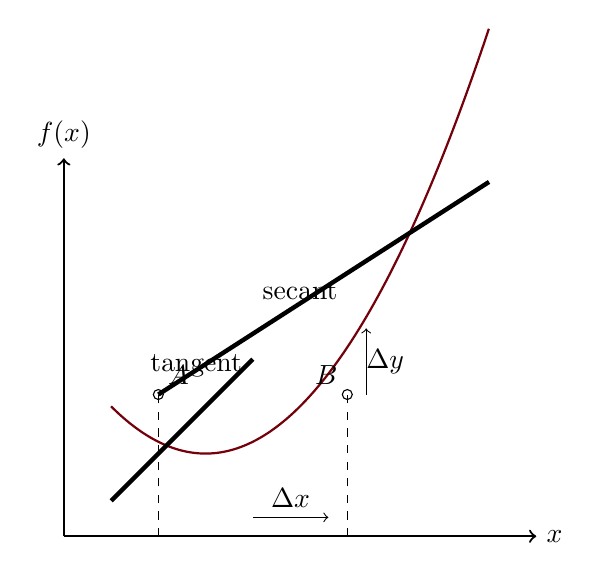
\begin{tikzpicture}[scale=1.2]
\draw[->, UofSCBlack, thick] (0,0) -- (5,0) node[right] {$x$};
\draw[->, UofSCBlack, thick] (0,0) -- (0,4) node[above] {$f(x)$};

\draw[UofSCGarnet, thick, domain=0.5:4.5, samples=100] plot (\x, {0.5*\x*\x - 1.5*\x + 2});

\draw[UofSCBlack, dashed] (1,0) -- (1,1.5);
\draw[UofSCBlack, dashed] (3,0) -- (3,1.5);

\draw[UofSCBlack] (1,1.5) circle (1.5pt) node[above right] {$A$};
\draw[UofSCBlack] (3,1.5) circle (1.5pt) node[above left] {$B$};

\draw[UofSCBlack, ultra thick] (1,1.5) -- (4.5,3.75);
\draw[UofSCBlack, ultra thick] (0.5,0.375) -- (2,1.875);

\draw[UofSCBlack] (2.5,2.6) node {secant};
\draw[UofSCBlack] (1.4,1.8) node {tangent};

\draw[->, UofSCBlack] (2,0.2) -- (2.8,0.2);
\draw[UofSCBlack] (2.4,0.4) node {$\Delta x$};

\draw[->, UofSCBlack] (3.2,1.5) -- (3.2,2.2);
\draw[UofSCBlack] (3.4,1.85) node {$\Delta y$};

\end{tikzpicture}
\caption{Geometric interpretation of the derivative: the slope of the secant line between two points approaches the slope of the tangent line as the points converge.}
\end{figure}

From a geometric perspective, the derivative at a point represents the slope of the tangent line to the function's graph at that point. To understand this, imagine selecting two distinct points $A$ and $B$ on a curve $y = f(x)$, with coordinates $A = (x_1, f(x_1))$ and $B = (x_2, f(x_2))$. The line passing through these two points is called a secant line, and its slope is given by the familiar rise-over-run formula $\frac{\Delta y}{\Delta x} = \frac{f(x_2) - f(x_1)}{x_2 - x_1}$. This slope represents the average rate of change of $f$ between $x_1$ and $x_2$. Now imagine sliding point $B$ closer and closer to point $A$, so that the distance $\Delta x = x_2 - x_1$ becomes increasingly small. As this distance approaches zero, the secant line rotates and converges to a single line that just touches the curve at point $A$ without crossing through it. This limiting line is the tangent line at $x_1$, and its slope is exactly the derivative $f'(x_1)$.

To make this precise, the derivative is defined as a limit. If we let $h$ represent the small distance between $x_1$ and $x_2$, so that $x_2 = x_1 + h$, then the secant slope becomes $\frac{f(x_1 + h) - f(x_1)}{h}$. The derivative is what this expression approaches as $h$ becomes arbitrarily small:

\[
f'(x_1) = \lim_{h \to 0} \frac{f(x_1 + h) - f(x_1)}{h}.
\]

This limit may not exist for all functions at all points, and those functions for which it does exist everywhere are called differentiable. Throughout our study of dynamic systems, we will work primarily with differentiable functions because their derivatives tell us how the system evolves.

From a physical perspective, the derivative has an immediate and intuitive meaning when our function describes a quantity changing over time. If $p(t)$ represents the position of our car at time $t$, then the derivative $p'(t)$ represents the instantaneous velocity of the car at that moment. Velocity is precisely the rate at which position changes with respect to time. If we measure position in meters and time in seconds, then velocity is measured in meters per second. When the car is moving forward, its velocity is positive; when it reverses direction, its velocity becomes negative. When the car comes to a complete stop at a traffic light, its velocity is zero. The derivative captures all of these physical realities directly.

To see this connection clearly, consider the average velocity of the car between time $t_1$ and time $t_2$. This average is simply the total change in position divided by the total change in time: $v_{\text{avg}} = \frac{p(t_2) - p(t_1)}{t_2 - t_1}$. This is exactly the same formula as the secant slope we encountered in the geometric interpretation. The instantaneous velocity at time $t_1$ is what this average velocity approaches as we make the time interval smaller and smaller, which is precisely the limit definition of the derivative $p'(t_1)$. Thus, the derivative unifies our geometric and physical intuitions: it is both the slope of the tangent line and the instantaneous velocity.

\begin{table}[htbp]
\centering
\begin{tabular}{|c|c|c|c|}
\hline
\rowcolor{UofSCGarnet}
\textcolor{white}{\textbf{Quantity}} & \textcolor{white}{\textbf{Symbol}} & \textcolor{white}{\textbf{Units}} & \textcolor{white}{\textbf{Interpretation}} \\
\hline
Position & $p(t)$ & meters (m) & Where the car is \\
\hline
Velocity & $p'(t)$ & meters per second (m/s) & How fast position changes \\
\hline
Acceleration & $p''(t)$ & meters per second squared (m/s$^2$) & How fast velocity changes \\
\hline
Jerk & $p'''(t)$ & meters per second cubed (m/s$^3$) & How fast acceleration changes \\
\hline
\end{tabular}
\captionsetup{type=table}
\caption{Derivatives of position and their physical interpretations.}
\end{table}

Beyond velocity, we can consider higher-order derivatives. The derivative of velocity with respect to time is acceleration, denoted $a(t) = p''(t)$, which tells us how quickly the car's speed is increasing or decreasing. The derivative of acceleration is called jerk, which measures how abruptly the acceleration is changing. While these higher-order derivatives are important in many applications, the fundamental insight is that each derivative represents a rate of change of the quantity described by the previous derivative.

From an algebraic perspective, the derivative provides a powerful tool for approximation. Near any point where a function is differentiable, the function can be approximated by a linear function whose slope matches the derivative. This is called the linear approximation or tangent line approximation of the function at that point. If we wish to approximate the value of $f(x)$ near a known point $x = a$, where we know both $f(a)$ and $f'(a)$, we use the formula:

\[
f(x) \approx f(a) + f'(a)(x - a).
\]

This formula says that to estimate $f(x)$, we start at the known value $f(a)$ and add the change that would occur if the function continued to change at its instantaneous rate $f'(a)$ over the distance $x - a$. The expression $f'(a)(x - a)$ represents the linear correction based on the derivative.

Let us work through a complete example to see how this approximation works in practice. Consider the function $f(x) = \sqrt{x}$, which gives the square root of $x$. Suppose we know that $\sqrt{4} = 2$, and we wish to estimate $\sqrt{4.1}$, which is close to 4. First, we compute the derivative of $f(x)$. Using the power rule, $f'(x) = \frac{1}{2\sqrt{x}}$. Evaluating at $a = 4$, we find $f'(4) = \frac{1}{2 \cdot 2} = \frac{1}{4} = 0.25$. Now applying the linear approximation formula:

\[
\sqrt{4.1} \approx \sqrt{4} + \frac{1}{4}(4.1 - 4) = 2 + 0.25 \cdot 0.1 = 2 + 0.025 = 2.025.
\]

To verify this approximation, we can compute the exact value. Using a calculator, $\sqrt{4.1} \approx 2.0248457$. Our approximation of $2.025$ is remarkably accurate, with an error of only about $0.00015$. This demonstrates the power of linear approximation: by knowing the function's value and its rate of change at a single point, we can accurately predict nearby values. The closer our target point is to the known point, the better the approximation becomes.

Now we connect these mathematical concepts to the study of dynamic systems. A dynamic system is a mathematical model that describes how a quantity evolves over time. The central insight of dynamic systems is that the rate of change of the system's state depends on the current state itself and possibly on external inputs. In the language of calculus, this means that the derivative of the state variable is a function of the state variable and any inputs.

For our car example, the position $p(t)$ is the state of the system. The rate of change of position, which is velocity $p'(t)$, depends on the current state (the car's speed and direction) and on external inputs (the driver's acceleration or braking). A complete model of the car's motion would express how the velocity changes based on these factors. For instance, if the driver presses the accelerator, velocity increases; if the driver brakes, velocity decreases; if the car encounters a hill, gravity affects both velocity and position.

This relationship between rates of change and current state is the fundamental structure that will govern our entire study of control systems. We will frequently encounter equations of the form:

\[
\frac{dx}{dt} = f(x, u, t),
\]

where $x$ represents the state of the system, $u$ represents external inputs, $t$ represents time, and $f$ is some function that describes how the rate of change depends on these quantities. Solving such equations—determining how the state $x$ evolves given its rate of change—requires the tools of differential equations, which we will develop in subsequent sections.

To solidify this connection, consider a simple dynamic system where a cup of hot coffee cools down over time. Let $T(t)$ represent the temperature of the coffee at time $t$, measured in degrees Celsius above room temperature. Experience tells us that the coffee cools faster when it is hotter and slower as it approaches room temperature. A simple model for this cooling is given by Newton's Law of Cooling:

\[
\frac{dT}{dt} = -kT,
\]

where $k$ is a positive constant that depends on properties of the cup and the coffee. This equation states that the rate of temperature change is proportional to the current temperature above room temperature, with the negative sign indicating that the temperature decreases. Here, the rate of change $\frac{dT}{dt}$ depends only on the current state $T$, with no external input. This is an autonomous dynamic system, and we will learn how to solve such equations to predict the coffee's temperature at any future time.

In summary, functions describe relationships between quantities, derivatives describe how those quantities change, and dynamic systems describe how rates of change depend on current states and inputs. This framework—the language of functions and their derivatives—provides the mathematical foundation for understanding and designing control systems that regulate the behavior of physical, biological, and engineered systems.


\subsection{Differential Equations --- Describing How Things Evolve}
\label{sec:differential_equations}

\subsection{Differential Equations — Describing How Things Evolve}

The behavior of every dynamic system in our world can be described by a single mathematical framework: the differential equation. When we ask questions like "How does the temperature in this room change over the next hour?" or "What happens to the car's speed when I press the accelerator?" or "How will the drone's orientation respond to my control inputs?", we are fundamentally asking how some quantity changes with respect to another. This relationship between rates of change and system behavior is precisely what differential equations capture. In control systems engineering, ordinary differential equations (ODEs) serve as the universal language through which we describe, analyze, and ultimately predict the evolution of physical, electrical, mechanical, and even economic systems over time.

An ordinary differential equation relates a function to its derivatives, expressing how the rate of change of a quantity depends on the current state of the system, on external inputs, and on fixed system parameters. The independent variable in almost all control systems problems is time, which we denote by $t$ and measure in seconds, minutes, or hours depending on the application. The dependent variables are the quantities that change with time—these are called the \emph{states} of the system. States might include position, velocity, temperature, voltage, current, pressure, or any other measurable quantity that evolves as time progresses. Parameters, in contrast, are fixed values that characterize the system itself: a resistor's resistance, a spring's stiffness, a motor's torque constant, or a thermal mass's heat capacity. Parameters define \emph{what} the system is, while states describe \emph{how} the system is behaving at any given moment.

The \emph{order} of a differential equation is determined by the highest derivative that appears in the equation. This seemingly simple classification has profound implications for system behavior, as different orders exhibit fundamentally different dynamic characteristics. A first-order differential equation relates the first derivative of a state variable to the state itself and possibly to external inputs. Mathematically, a general first-order ODE takes the form $\dot{x}(t) = f(x(t), u(t), \theta)$, where $\dot{x}$ denotes the time derivative $dx/dt$, $x$ is the state variable, $u$ represents external inputs, and $\theta$ collects all system parameters. The physical interpretation is straightforward: the rate at which the state changes depends on its current value and on whatever external influences are acting on the system. First-order systems have no memory beyond their current state—their entire future behavior is completely determined by knowing their present state and any future inputs.

To build intuition, consider a simple resistor-capacitor (RC) circuit. A capacitor of capacitance $C$ stores electrical charge, and a resistor of resistance $R$ limits the flow of current. When we connect this circuit to a voltage source $V_s$, charge flows onto the capacitor, causing its voltage $v_C$ to rise over time. The relationship between the capacitor voltage and time follows directly from Kirchhoff's voltage law and the definition of capacitor behavior. The current through the capacitor equals the rate of change of charge, $i_C = C \, dv_C/dt$, and by Ohm's law the current through the resistor equals the voltage drop across it divided by its resistance, $i_R = (V_s - v_C)/R$. Since the same current flows through both components in series, we equate these expressions:

\begin{equation}
C \frac{dv_C}{dt} = \frac{V_s - v_C}{R}.
\end{equation}

Rearranging this equation into standard form gives us the first-order differential equation governing the capacitor voltage:

\begin{equation}
\frac{dv_C}{dt} + \frac{1}{RC} v_C = \frac{1}{RC} V_s.
\end{equation}

This equation tells us that the rate of change of capacitor voltage is proportional to the difference between the source voltage and the current capacitor voltage. When $v_C$ is much smaller than $V_s$, the rate of change is large and the capacitor charges quickly. As $v_C$ approaches $V_s$, the rate of change diminishes, and the voltage asymptotically approaches its steady-state value. The product $RC$, with units of seconds, is called the \emph{time constant} of the circuit and characterizes how rapidly the system responds. A smaller time constant means faster dynamics—a system that reaches equilibrium more quickly.

\begin{table}[h]
\centering
\begin{tabular}{|c|c|c|c|}
\hline
\textbf{Physical System} & \textbf{State Variable} & \textbf{First-Order ODE} & \textbf{Time Constant} \\
\hline
RC Circuit & Capacitor voltage $v_C$ & $\dot{v}_C = \frac{V_s - v_C}{RC}$ & $\tau = RC$ \\
\hline
Thermal System & Temperature $T$ & $\dot{T} = \frac{T_{\text{env}} - T}{RC_{\text{th}}}$ & $\tau = R C_{\text{th}}$ \\
\hline
Hydraulic Tank & Fluid height $h$ & $\dot{h} = \frac{Q_{\text{in}} - Q_{\text{out}}}{A}$ & $\tau = \frac{A}{k_{\text{out}}}$ \\
\hline
DC Motor & Angular velocity $\omega$ & $\dot{\omega} = \frac{K_t V - B\omega}{J}$ & $\tau = \frac{J}{B}$ \\
\hline
\end{tabular}
\vspace{0.5cm}
\caption{First-order systems from diverse physical domains share a common mathematical structure. Each system exhibits exponential approach to steady state with behavior characterized by a single time constant.}
\label{tab:first_order_systems}
\end{table}

Thermal systems provide another illuminating example of first-order dynamics. Imagine a room of thermal mass $C_{\text{th}}$ (measured in J/°C) that exchanges heat with the outside environment through walls and windows that have a combined thermal resistance $R_{\text{th}}$ (measured in °C/W). If the outside temperature is $T_{\text{env}}$ and the room temperature is $T$, the rate of heat flow into the room equals $(T_{\text{env}} - T)/R_{\text{th}}$. This heat flow causes the room temperature to rise at a rate given by the heat capacity: $\dot{T} = \frac{1}{C_{\text{th}}} \cdot \frac{T_{\text{env}} - T}{R_{\text{th}}}$. The governing differential equation is therefore

\begin{equation}
\dot{T} = \frac{T_{\text{env}} - T}{R_{\text{th}} C_{\text{th}}}.
\end{equation}

Again we see the characteristic first-order structure: the rate of change of the state variable (temperature) is proportional to the difference between the current state and the external forcing (ambient temperature). The product $R_{\text{th}} C_{\text{th}}$ is the thermal time constant, determining how many minutes or hours the room requires to heat up or cool down significantly. Table~\ref{tab:first_order_systems} summarizes several common first-order physical systems, demonstrating the remarkable mathematical unity underlying diverse physical phenomena.

Second-order differential equations relate the second derivative of a state variable to lower-order terms, introducing a fundamentally new characteristic: oscillatory behavior. A general second-order ODE takes the form $\ddot{x}(t) = f(x(t), \dot{x}(t), u(t), \theta)$, where $\ddot{x}$ denotes the second derivative $d^2x/dt^2$. The presence of the second derivative means that the acceleration of the state depends on both its position (first derivative, which is velocity in mechanical systems) and its displacement. This coupling between position and velocity creates the possibility of energy storage in two different forms, which can be exchanged back and forth to produce oscillations.

The canonical example of second-order dynamics is the mass-spring-damper system. A mass $m$ is connected to a spring of stiffness $k$ and a damper with damping coefficient $b$, and may be subjected to an external force $F(t)$. Newton's second law states that the sum of forces equals mass times acceleration: $\sum F = m \ddot{x}$, where $x$ is the displacement of the mass from its equilibrium position. The spring exerts a restoring force $-k x$ (negative because it opposes displacement), the damper produces a dissipative force $-b \dot{x}$ (proportional to velocity), and the external force $F$ drives the system. Applying Newton's law gives:

\begin{equation}
m \ddot{x} + b \dot{x} + k x = F(t).
\end{equation}

This equation is the archetype of linear second-order systems and appears throughout mechanical, civil, aerospace, and structural engineering. The behavior of this system depends critically on the relative sizes of the three terms. If the damping coefficient $b$ is small relative to $\sqrt{mk}$, the system will oscillate with gradually decreasing amplitude when disturbed—the underdamped case. If $b$ is large, the mass returns to equilibrium without oscillating—the overdamped case. The boundary between these regimes, where $b = 2\sqrt{mk}$, is called critical damping and represents the fastest return to equilibrium without oscillation. These three regimes—underdamped, critically damped, and overdamped—characterize all second-order systems and profoundly influence control system design.

\begin{table}[h]
\centering
\begin{tabular}{|c|c|c|c|}
\hline
\textbf{Parameter} & \textbf{Symbol} & \textbf{Definition} & \textbf{Physical Meaning} \\
\hline
Natural frequency & $\omega_n$ & $\sqrt{\frac{k}{m}}$ (mechanical) or $\frac{1}{\sqrt{LC}}$ (electrical) & Oscillation frequency with no damping \\
\hline
Damping ratio & $\zeta$ & $\frac{b}{2\sqrt{mk}}$ (mechanical) or $\frac{R}{2}\sqrt{\frac{C}{L}}$ (electrical) & Measure of damping strength \\
\hline
Damped frequency & $\omega_d$ & $\omega_n \sqrt{1-\zeta^2}$ & Oscillation frequency when $\zeta < 1$ \\
\hline
\end{tabular}
\vspace{0.5cm}
\caption{The standard form of second-order systems introduces two dimensionless parameters—natural frequency and damping ratio—that completely characterize dynamic behavior across mechanical, electrical, and other physical domains.}
\label{tab:second_order_params}
\end{table}

The RLC circuit provides an electrical counterpart to the mass-spring-damper system and demonstrates the deep mathematical analogy between mechanical and electrical systems. An inductor of inductance $L$ stores energy in its magnetic field, a capacitor of capacitance $C$ stores energy in its electric field, and a resistor of resistance $R$ dissipates energy as heat. When we apply a voltage source $V(t)$ to this series circuit, Kirchhoff's voltage law gives $V(t) = v_L + v_R + v_C$. The voltage across the resistor is $v_R = R i$, the voltage across the capacitor is $v_C = \frac{1}{C} \int i \, dt$, and the voltage across the inductor is $v_L = L \, di/dt$. Substituting these expressions and differentiating to eliminate the integral yields:

\begin{equation}
L \ddot{q} + R \dot{q} + \frac{1}{C} q = V(t),
\end{equation}

where $q$ is the charge on the capacitor. Recognizing that current $i = \dot{q}$, we can write this in terms of current as:

\begin{equation}
L \frac{di}{dt} + R i + \frac{1}{C} \int i \, dt = V(t).
\end{equation}

This equation has precisely the same mathematical structure as the mass-spring-damper equation: an inertial term proportional to the second derivative, a dissipative term proportional to the first derivative, and a restorative term proportional to the state itself. This is no coincidence—it reflects a fundamental mathematical analogy that allows engineers to translate insights between mechanical and electrical domains. Table~\ref{tab:second_order_params} defines the standard parameters—natural frequency $\omega_n$ and damping ratio $\zeta$—that characterize all second-order systems regardless of their physical implementation.

Higher-order systems, those whose governing equations involve third or higher derivatives, arise whenever there are three or more independent energy storage elements or when the system has distributed parameters (like a long transmission line where electrical effects propagate along its length). While more complex mathematically, higher-order systems can always be decomposed into multiple first- and second-order subsystems connected in some configuration. Understanding first- and second-order systems therefore provides the foundation for analyzing systems of any order.

Solving a differential equation means finding the function $x(t)$ that satisfies the equation for all time, subject to initial conditions that specify the system state at some starting time. Geometrically, this solution is a \emph{trajectory}—a path through the state space that the system follows as time progresses. For a first-order system, the state space is one-dimensional, so the trajectory is simply a curve on a line. The system starts at its initial state $x(0)$ and moves along the trajectory determined by the differential equation, never deviating from the path prescribed by $\dot{x} = f(x,u)$. For a second-order system with state variables $x_1$ and $x_2$ (for example, position and velocity), the state space is two-dimensional, and the solution traces a curve in this plane. The entire future behavior of the system is encoded in this trajectory—knowing the trajectory tells us the state of the system at every future time.

Consider the unforced ($F(t) = 0$) mass-spring-damper system with initial conditions $x(0) = x_0$ and $\dot{x}(0) = v_0$. In the underdamped case ($\zeta < 1$), the solution is

\begin{equation}
x(t) = e^{-\zeta \omega_n t} \left( x_0 \cos(\omega_d t) + \frac{v_0 + \zeta \omega_n x_0}{\omega_d} \sin(\omega_d t) \right),
\end{equation}

where $\omega_d = \omega_n \sqrt{1-\zeta^2}$ is the damped natural frequency. This trajectory spirals inward toward the origin in the phase plane (the plane with position and velocity as axes), reflecting the gradual dissipation of energy through the damper. The rate of this spiral—the speed at which energy is lost—is determined by the damping ratio $\zeta$, while the frequency of the spiral's rotation is determined by $\omega_d$. Every initial condition produces a different trajectory, but all trajectories share the same qualitative shape: exponential decay modulated by sinusoidal oscillation.

Understanding differential equations as descriptions of trajectories through state space provides the conceptual foundation for all of control systems engineering. When we design a controller, we are essentially sculpting the vector field that generates these trajectories—pushing the system along desired paths, steering it away from dangerous regions, and guiding it toward specified equilibrium points. The tools we develop throughout this text for analyzing, designing, and implementing control systems all build upon this fundamental connection between differential equations and dynamic behavior.


\subsection{Linear Superposition and the Power of Linear Systems}
\label{sec:linear_superposition}

\subsection{Linear Superposition and the Power of Linear Systems}

The universe has a remarkable property that makes the analysis of many physical systems tractable: causes add up and effects add up. When you push twice as hard on a door, it swings twice as far. When two people together lift a weight that neither could lift alone, their combined effort produces a result equal to the sum of their individual efforts. This seemingly simple observation is the foundation of linearity, and it unlocks extraordinary analytical power that pervades all branches of engineering and physics. Understanding the superposition principle is not merely an academic exercise—it is the key that unlocks the analysis of vibrating structures, electrical circuits, thermal systems, and virtually every control system we will encounter in this textbook.

The mathematical statement of linearity builds directly on this intuitive notion of additivity. Consider a system that transforms an input signal $x(t)$ into an output signal $y(t)$, which we denote compactally as $y(t) = \mathcal{L}\{x(t)\}$ where $\mathcal{L}$ represents the system's behavior. This system is linear if it satisfies two fundamental properties for all possible inputs and for all constants $a$ and $b$. First, homogeneity (also called scaling) requires that scaling the input by a constant scales the output by the same constant: if $y_1(t) = \mathcal{L}\{x_1(t)\}$, then $\mathcal{L}\{a x_1(t)\} = a y_1(t)$. Second, additivity requires that the response to the sum of two inputs equals the sum of their individual responses: if $y_2(t) = \mathcal{L}\{x_2(t)\}$, then $\mathcal{L}\{x_1(t) + x_2(t)\} = y_1(t) + y_2(t)$. These two properties are often combined into a single statement called the superposition principle:

\begin{equation}
\mathcal{L}\{a x_1(t) + b x_2(t)\} = a \mathcal{L}\{x_1(t)\} + b \mathcal{L}\{x_2(t)\}.
\end{equation}

This equation tells us that a linear system cannot create new frequency components, cannot generate harmonics from sinusoidal inputs, and cannot produce outputs that grow faster than their inputs. More importantly for our purposes, it tells us that we can analyze complex inputs by breaking them into simple pieces, analyzing each piece separately, and then adding the results together.

To develop intuition for why linearity is so powerful, consider what happens when you cannot use superposition. Suppose you face a nonlinear differential equation describing a system where the force contains a term proportional to the square of velocity, as occurs in aerodynamic drag. When you double the input force, the output does not double because the drag force changes quadratically with velocity. When you combine two different inputs, their interaction terms create cross-products that make the total response different from the sum of individual responses. Each new input combination produces a qualitatively new behavior that requires entirely new analysis. The system resists decomposition into simpler problems.

Linear systems, by contrast, surrender their secrets willingly. Any complex input can be expressed as a sum of simpler basis functions—whether these are sines and cosines in Fourier analysis, decaying exponentials in Laplace analysis, or any other complete set of functions that spans the space of possible inputs. Because of superposition, the response to the complex input is simply the sum of the responses to each basis function. We analyze each basis function in isolation (often finding simple closed-form expressions for their responses), then add the pieces together to obtain the complete solution. This decomposition-recombination strategy is the essence of linear system analysis and appears in virtually every technique we will develop throughout this textbook.

The decomposition strategy leads naturally to the distinction between homogeneous and particular solutions, which represent two fundamentally different types of system responses. The homogeneous solution (also called the natural response or transient response) describes how the system behaves when left to itself, responding only to its initial conditions. For a mass-spring-damper system released from some initial displacement with some initial velocity, the homogeneous solution captures the oscillations that naturally occur as energy transfers back and forth between the spring and the mass, gradually dissipating through the damper. The particular solution (also called the forced response or steady-state response) describes how the system is driven by external inputs, assuming we wait long enough for any natural oscillations to die out. The complete solution is always the sum of these two components:

\begin{equation}
y(t) = y_h(t) + y_p(t),
\end{equation}

where $\mathcal{L}\{y_h(t)\} = 0$ and $\mathcal{L}\{y_p(t)\} = x(t)$. The homogeneous solution encodes the system's intrinsic character—its natural frequencies, damping characteristics, and stability properties—while the particular solution encodes how the system responds to specific external driving forces. Both pieces are essential for a complete understanding, and both can be found using linear techniques.

\begin{table}[htbp]
\centering
\begin{tabular}{|l|c|c|c|}
\hline
\textbf{Domain} & \textbf{Storage Element} & \textbf{Dissipative Element} & \textbf{Linear System Equation} \\
\hline
Mechanical & Mass ($M$) & Damper ($B$) & $M\ddot{x} + B\dot{x} + Kx = F(t)$ \\
\hline
Electrical & Inductor ($L$) / Capacitor ($C$) & Resistor ($R$) & $L\frac{dI}{dt} + RI + \frac{1}{C}\int I\,dt = V(t)$ \\
\hline
Thermal & Thermal Mass ($C_{th}$) & Thermal Resistance ($R_{th}$) & $C_{th}\frac{dT}{dt} + \frac{T - T_{amb}}{R_{th}} = \dot{Q}(t)$ \\
\hline
\end{tabular}
\vskip 0.5em
\color{UofSCBlack}\footnotesize \textbf{Table 1.1:} Linear system equations across different physical domains share a common structure: storage elements (mass, inductance, capacitance, thermal mass) produce derivative terms, dissipative elements (damper, resistor, thermal resistance) produce algebraic terms, and the sum equals the forcing function.
\end{table}

The universality of linear analysis becomes apparent when we recognize the same mathematical structure appearing across fundamentally different physical domains. Table 1.1 illustrates this correspondence, showing how mechanical translational systems, electrical circuits, and thermal systems all obey linear differential equations of the same general form. A mechanical engineer analyzing a car's suspension system and an electrical engineer analyzing a radio tuned circuit are solving the same mathematics, just with different variable names and units. This mathematical unity is not coincidental—it reflects deep physical principles about energy storage and dissipation that transcend any particular domain. When you master linear analysis in one domain, you master it in all domains.

To make these abstract ideas concrete, let us work through a detailed example involving a mass-spring-damper system, which is the canonical model for many mechanical control problems. Consider a mass $M = 2$ kg attached to a spring with stiffness $K = 8$ N/m and a damper with coefficient $B = 4$ N·s/m. The differential equation governing this system is:

\begin{equation}
2\ddot{x} + 4\dot{x} + 8x = F(t),
\end{equation}

where $x(t)$ is the displacement of the mass from its equilibrium position and $F(t)$ is an external force applied to the mass. We wish to find the complete response when the system starts at $x(0) = 0.1$ m with zero initial velocity $\dot{x}(0) = 0$, and is then subjected to a step force $F(t) = 8$ N applied at $t = 0$.

We begin by finding the homogeneous solution, which satisfies $2\ddot{x}_h + 4\dot{x}_h + 8x_h = 0$. Assuming solutions of the form $x_h(t) = e^{st}$, we substitute to obtain the characteristic equation $2s^2 + 4s + 8 = 0$, which simplifies to $s^2 + 2s + 4 = 0$. The roots are $s = -1 \pm i\sqrt{3}$, which have negative real parts, indicating a stable system that will settle to equilibrium. The homogeneous solution is therefore:

\begin{equation}
x_h(t) = e^{-t}\left(A \cos(\sqrt{3}\,t) + B \sin(\sqrt{3}\,t)\right),
\end{equation}

where $A$ and $B$ are constants determined by initial conditions.

Next, we find the particular solution for the constant forcing function $F(t) = 8$ N. Since the forcing function is constant and the system is stable, we expect the particular solution to also be constant: $x_p(t) = C$. Substituting into the differential equation gives $2(0) + 4(0) + 8C = 8$, so $C = 1$. The particular solution is simply $x_p(t) = 1$ meter.

The complete solution is $x(t) = x_h(t) + x_p(t)$, and we determine the constants $A$ and $B$ by applying the initial conditions. At $t = 0$, $x(0) = x_h(0) + x_p(0) = (A)(1) + 1 = A + 1$. Since $x(0) = 0.1$, we have $A = -0.9$. The velocity is $\dot{x}(t) = \dot{x}_h(t) + \dot{x}_p(t)$, and since $x_p(t) = 1$ is constant, $\dot{x}_p(t) = 0$. Differentiating $x_h(t)$ gives:

\begin{equation}
\dot{x}_h(t) = -e^{-t}\left(A \cos(\sqrt{3}\,t) + B \sin(\sqrt{3}\,t)\right) + e^{-t}\left(-A\sqrt{3}\sin(\sqrt{3}\,t) + B\sqrt{3}\cos(\sqrt{3}\,t)\right).
\end{equation}

At $t = 0$, $\dot{x}_h(0) = -A + B\sqrt{3} = -(-0.9) + B\sqrt{3} = 0.9 + B\sqrt{3}$. Since $\dot{x}(0) = 0$, we have $0.9 + B\sqrt{3} = 0$, so $B = -0.9/\sqrt{3} = -0.3\sqrt{3}$.

The complete response is therefore:

\begin{equation}
x(t) = 1 - 0.9e^{-t}\left(\cos(\sqrt{3}\,t) + \sqrt{3}\sin(\sqrt{3}\,t)\right).
\end{equation}

This solution beautifully illustrates the decomposition into homogeneous and particular components. The particular solution $x_p(t) = 1$ represents the steady-state displacement that the mass eventually approaches as the transient oscillations die out. The homogeneous solution represents an oscillatory transient that decays exponentially with time constant $\tau = 1$ second, completely determined by the system's natural dynamics rather than by the applied force. The superposition principle allowed us to find these two components independently and then simply add them together to obtain the complete solution.

The electrical analog of this mechanical system provides another perspective on the same mathematics. Consider a series RLC circuit with resistance $R = 4$ $\Omega$, inductance $L = 2$ H, and capacitance $C = 0.25$ F, driven by a voltage source $V(t) = 8$ V applied at $t = 0$. The differential equation for the capacitor voltage $v_C(t)$ is:

\begin{equation}
2\ddot{v}_C + 4\dot{v}_C + 8v_C = 8,
\end{equation}

which is mathematically identical to the mechanical system we just analyzed. If the capacitor initially has voltage $v_C(0) = 0.1$ V and the initial current through the inductor is zero, the solution for $v_C(t)$ is identical in form to our mechanical solution: the capacitor voltage will approach the steady-state value of 1 V while exhibiting damped oscillations at frequency $\sqrt{3}$ rad/s with exponential decay at rate 1/s. The correspondence is not superficial—it reflects the fact that energy stored in the mechanical system's spring (potential energy) corresponds to energy stored in the capacitor's electric field, energy stored in the mass's motion corresponds to energy stored in the inductor's magnetic field, and energy dissipated by the damper corresponds to energy dissipated as heat in the resistor.

The power of superposition extends far beyond these simple examples to encompass the entire frequency-domain analysis that forms the backbone of classical control theory. When we decompose a periodic input into its Fourier series components, we can analyze the system's response to each sinusoidal component separately, then add the responses together. When we use the Laplace transform to analyze transients, we are decomposing arbitrary inputs into exponentially weighted sinusoids (the complex frequencies $s = \sigma + j\omega$) and analyzing each component separately. When we use state-space methods to analyze multi-input multi-output systems, we are implicitly exploiting linearity to decouple the equations through similarity transformations. Every major technique in control theory is, at its core, an application of the superposition principle.

However, we must be honest about the limitations of linear analysis. Many real systems exhibit nonlinear behavior that cannot be ignored. A pendulum becomes nonlinear for large angles. Transistors operate in regimes where their characteristic curves are highly nonlinear. Friction in mechanical systems often follows laws (like Coulomb friction) that are fundamentally nonlinear. For these systems, superposition fails: doubling the input does not double the output, and the response to two inputs is not the sum of their individual responses. Nonlinear systems can exhibit phenomena impossible in linear systems: limit cycles, chaos, hysteresis, and jump resonance. Understanding linear systems is essential precisely because it provides the foundation from which we can recognize and approximately analyze nonlinear systems, and because many systems can be usefully modeled as linear within restricted operating ranges.

The strategy for analyzing linear systems that we will employ throughout this textbook follows a consistent pattern. First, we model the physical system using linear differential equations or linear state-space equations. Second, we decompose the problem using transform methods (Laplace, Fourier, or z-transform) or using modal analysis in the time domain. Third, we analyze each component of the decomposition independently, exploiting superposition. Fourth, we recombine the component responses to obtain the complete solution. Fifth, we interpret the results physically and assess whether the linear model remains valid. This methodology, built entirely on the superposition principle, gives us extraordinary analytical power for understanding and designing control systems.

As we proceed through subsequent chapters, the superposition principle will become so ingrained in our thinking that we will apply it almost unconsciously. When we analyze the steady-state response to sinusoidal inputs using frequency response methods, we are using superposition. When we design controllers by placing poles in desired locations, we are using the linearity that ensures pole locations determine system behavior independently of inputs. When we use state observers to estimate system states from outputs, we are using linearity to decouple the estimation problem from the control problem. The investment we make in thoroughly understanding superposition now will pay dividends throughout our study of control systems.


\subsection{Complex Numbers and Frequency Domain Thinking}
\label{sec:complex_numbers}

\subsection{Complex Numbers and Frequency Domain Thinking}

The analysis of control systems invariably involves quantities that oscillate, vibrate, and repeat over time. Before we can understand how controllers shape the behavior of dynamic systems, we must develop a mathematical language capable of describing oscillatory motion with elegance and simplicity. This language is built upon complex numbers, and the purpose of this subsection is to develop the geometric and algebraic intuition necessary to use complex numbers as a tool for control system analysis. What may initially appear as an abstract mathematical detour will prove to be the cornerstone of everything that follows, transforming the seemingly intractable problem of solving differential equations into straightforward algebraic manipulations.

\subsubsection{The Geometric View: Numbers as Points in a Plane}

Our familiar real numbers can be visualized as points along a straight line, where each position corresponds to a specific value. This one-dimensional number line serves well for representing quantities like temperature, velocity, or mass, but it fails entirely to capture the essential character of oscillatory phenomena. When a mass bobs up and down on a spring, it moves through a cycle of positions that repeats endlessly. When an alternating current flows through a wire, the voltage rises and falls in a rhythmic pattern. These behaviors are fundamentally two-dimensional in nature, involving both a magnitude and a direction of rotation or phase.

A complex number provides precisely this two-dimensional representation. We define a complex number $z$ as an ordered pair of real numbers $(a, b)$, which we write in the standard form $z = a + jb$ where $j$ represents the imaginary unit satisfying $j^2 = -1$. The term $a$ is called the real part of $z$, denoted $\operatorname{Re}\{z\}$, and $b$ is called the imaginary part, denoted $\operatorname{Im}\{z\}$. To visualize a complex number, we construct the complex plane, shown in Figure~\ref{fig:complex_plane}, where the horizontal axis represents the real component and the vertical axis represents the imaginary component. Every complex number corresponds to exactly one point in this plane, and conversely, every point in the complex plane corresponds to exactly one complex number.

\begin{figure}[htbp]
    \centering
    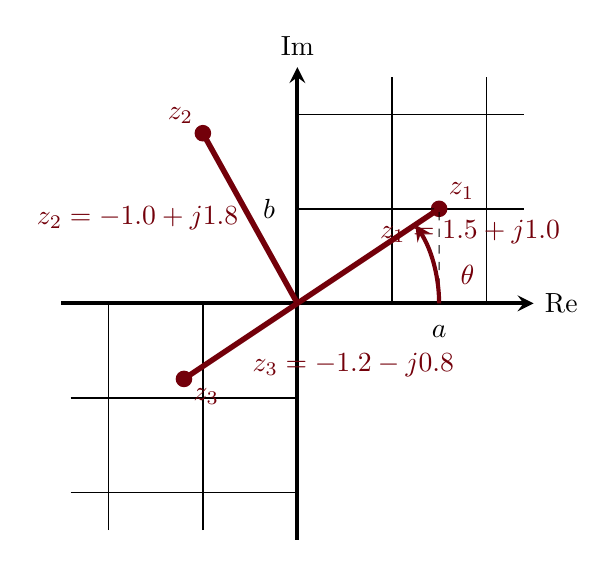
\begin{tikzpicture}[scale=1.2, >=stealth]
        \draw[->, UofSCBlack, line width=1.5pt] (-2.5, 0) -- (2.5, 0) node[right] {$\operatorname{Re}$};
        \draw[->, UofSCBlack, line width=1.5pt] (0, -2.5) -- (0, 2.5) node[above] {$\operatorname{Im}$};
        \draw[UofSCBlack, line width=0.5pt] (0,0) grid (2.4,2.4);
        \draw[UofSCBlack, line width=0.5pt] (0,0) grid (-2.4,-2.4);

        \coordinate (z1) at (1.5, 1.0);
        \coordinate (z2) at (-1.0, 1.8);
        \coordinate (z3) at (-1.2, -0.8);

        \draw[UofSCGarnet, line width=2pt] (0,0) -- (z1) node[midway, above right] {$z_1 = 1.5 + j1.0$};
        \draw[UofSCGarnet, line width=2pt] (0,0) -- (z2) node[midway, left] {$z_2 = -1.0 + j1.8$};
        \draw[UofSCGarnet, line width=2pt] (0,0) -- (z3) node[midway, below right] {$z_3 = -1.2 - j0.8$};

        \fill[UofSCGarnet] (z1) circle (2.5pt) node[above right] {$z_1$};
        \fill[UofSCGarnet] (z2) circle (2.5pt) node[above left] {$z_2$};
        \fill[UofSCGarnet] (z3) circle (2.5pt) node[below right] {$z_3$};

        \draw[UofSCBlack, dashed] (1.5, 0) -- (z1) -- (0, 1.0);
        \node[UofSCBlack] at (1.5, -0.3) {$a$};
        \node[UofSCBlack] at (-0.3, 1.0) {$b$};

        \draw[UofSCGarnet, ->, line width=1.5pt] (1.5, 0) arc (0:33.69:1.5);
        \node[UofSCGarnet] at (1.8, 0.3) {$\theta$};
    \end{tikzpicture}
    \caption{The complex plane represents complex numbers as points. Each complex number $z = a + jb$ corresponds to a point with real coordinate $a$ and imaginary coordinate $b$. The angle $\theta$ and radius $r$ provide an alternative polar representation.}
    \label{fig:complex_plane}
\end{figure}

Beyond representing points, complex numbers encode a profound geometric operation: rotation. Consider what happens when we multiply a complex number by $j$. If we begin with $z = a + jb$, then $jz = j(a + jb) = ja + j^2b = -b + ja$. This transformation moves the point $(a, b)$ to $(-b, a)$, which geometrically represents a counterclockwise rotation of 90 degrees about the origin. Multiplying by $j$ again gives $j^2z = j(-b + ja) = -jb + j^2a = -a - jb$, which corresponds to a 180-degree rotation. A third multiplication gives $j^3z = j(-a - jb) = -ja - j^2b = b - ja$, and finally $j^4z = j(b - ja) = jb - j^2a = a + jb$, returning us to the original point after a complete 360-degree rotation. This extraordinary property—that multiplication by $j$ corresponds to a right angle rotation—lies at the heart of why complex numbers prove so useful for describing oscillatory phenomena. An oscillation, after all, is precisely a rotation in a two-dimensional space where only one dimension (the real axis) is physically observable.

\subsubsection{Polar Form and Euler's Formula}

While the rectangular form $z = a + jb$ proves convenient for addition and subtraction, the polar form provides tremendous advantages for multiplication, division, and especially for describing oscillatory behavior. Any complex number $z = a + jb$ can be expressed as $z = re^{j\theta}$, where $r = \sqrt{a^2 + b^2}$ is the magnitude (or modulus) of $z$, and $\theta = \arctan(b/a)$ is the angle (or argument) of $z$ measured counterclockwise from the positive real axis. This representation connects directly to our geometric intuition: $r$ tells us how far the point lies from the origin, while $\theta$ tells us in which direction.

The equivalence between rectangular and polar forms rests upon one of the most remarkable identities in all of mathematics, known as Euler's formula:
\begin{equation}
e^{j\theta} = \cos\theta + j\sin\theta.
\end{equation}
This formula, proven by the Swiss mathematician Leonhard Euler in the eighteenth century, establishes an unexpected bridge between exponential functions and trigonometric functions through the vehicle of complex numbers. To verify Euler's formula intuitively, consider the Taylor series expansions of the exponential, cosine, and sine functions:
\begin{align}
e^x &= 1 + x + \frac{x^2}{2!} + \frac{x^3}{3!} + \frac{x^4}{4!} + \cdots, \\
\cos x &= 1 - \frac{x^2}{2!} + \frac{x^4}{4!} - \frac{x^6}{6!} + \cdots, \\
\sin x &= x - \frac{x^3}{3!} + \frac{x^5}{5!} - \frac{x^7}{7!} + \cdots.
\end{align}
Substituting $x = j\theta$ into the exponential series and grouping real and imaginary terms yields:
\begin{align}
e^{j\theta} &= 1 + j\theta + \frac{(j\theta)^2}{2!} + \frac{(j\theta)^3}{3!} + \frac{(j\theta)^4}{4!} + \cdots \\
&= 1 + j\theta - \frac{\theta^2}{2!} - j\frac{\theta^3}{3!} + \frac{\theta^4}{4!} + \cdots \\
&= \left(1 - \frac{\theta^2}{2!} + \frac{\theta^4}{4!} - \cdots\right) + j\left(\theta - \frac{\theta^3}{3!} + \frac{\theta^5}{5!} - \cdots\right) \\
&= \cos\theta + j\sin\theta.
\end{align}
The power of Euler's formula lies in how dramatically it simplifies operations that would otherwise be cumbersome. Multiplication of two complex numbers in rectangular form requires four multiplications and two additions:
\begin{equation}
(a + jb)(c + jd) = (ac - bd) + j(ad + bc).
\end{equation}
In polar form, however, multiplication reduces to multiplying the magnitudes and adding the angles:
\begin{equation}
(r_1 e^{j\theta_1})(r_2 e^{j\theta_2}) = r_1 r_2 e^{j(\theta_1 + \theta_2)}.
\end{equation}
Division becomes division of magnitudes and subtraction of angles. Raising a complex number to a power involves raising the magnitude to that power and multiplying the angle by the exponent. These algebraic simplifications directly mirror the geometric operations of scaling and rotating, and they prove indispensable when we analyze systems that oscillate at specific frequencies.

\subsubsection{Complex Exponentials and Oscillations}

We are now prepared to understand why complex numbers serve as the natural language for describing oscillatory motion. Consider the function $x(t) = A\cos(\omega t + \phi)$, which represents simple harmonic oscillation with amplitude $A$, angular frequency $\omega$, and phase shift $\phi$. This function describes the position of an idealized mass on a spring, the voltage of an alternating current, or countless other physical phenomena exhibiting repetitive behavior. Using Euler's formula, we can express this cosine function as the real part of a complex exponential:
\begin{equation}
A\cos(\omega t + \phi) = \operatorname{Re}\left\{A e^{j(\omega t + \phi)}\right\} = \operatorname{Re}\left\{A e^{j\phi} e^{j\omega t}\right\}.
\end{equation}
The complex quantity $\tilde{x}(t) = A e^{j\phi} e^{j\omega t}$ contains exactly the same information as the real function $x(t)$, but in a form that is dramatically easier to manipulate mathematically. The factor $A e^{j\phi}$ is a complex constant called the phasor (or complex amplitude), which encodes both the amplitude $A$ and the phase $\phi$ of the oscillation. The factor $e^{j\omega t}$ represents a point rotating counterclockwise around the origin of the complex plane at angular velocity $\omega$. Taking the real part of this rotating phasor at any time $t$ yields the physical oscillatory quantity.

The genius of this representation becomes apparent when we consider differentiation. Computing the derivative of the real cosine function requires applying the chain rule:
\begin{equation}
\frac{d}{dt}A\cos(\omega t + \phi) = -A\omega\sin(\omega t + \phi).
\end{equation}
The derivative of the complex exponential, however, follows directly from the differentiation rule for exponentials:
\begin{equation}
\frac{d}{dt}e^{j\omega t} = j\omega e^{j\omega t}.
\end{equation}
Differentiating a complex exponential simply multiplies it by the constant $j\omega$. This is the crucial observation that will transform our approach to control system analysis. The differential operator $\frac{d}{dt}$ acting on $e^{j\omega t}$ becomes an algebraic multiplication by the complex constant $j\omega$. If we represent all signals as the real parts of complex exponentials oscillating at various frequencies, differential equations become algebraic equations.

To see this transformation in action, consider the simple differential equation describing an undamped harmonic oscillator:
\begin{equation}
\ddot{x} + \omega_n^2 x = 0.
\end{equation}
We seek solutions of the form $x(t) = \operatorname{Re}\{\tilde{x}(t)\}$ where $\tilde{x}(t) = X e^{j\omega t}$ for some complex amplitude $X$. Computing the derivatives:
\begin{align}
\dot{x}(t) &= \operatorname{Re}\{j\omega X e^{j\omega t}\}, \\
\ddot{x}(t) &= \operatorname{Re}\{(j\omega)^2 X e^{j\omega t}\} = \operatorname{Re}\{-\omega^2 X e^{j\omega t}\}.
\end{align}
Substituting into the differential equation gives:
\begin{equation}
\operatorname{Re}\{-\omega^2 X e^{j\omega t}\} + \omega_n^2 \operatorname{Re}\{X e^{j\omega t}\} = \operatorname{Re}\{(-\omega^2 + \omega_n^2) X e^{j\omega t}\} = 0.
\end{equation}
For this to hold for all time $t$, the complex quantity in braces must be identically zero, which requires:
\begin{equation}
-\omega^2 + \omega_n^2 = 0 \quad\Rightarrow\quad \omega = \pm\omega_n.
\end{equation}
The solutions correspond to oscillations at the natural frequency $\omega_n$, exactly as expected. The general solution is $x(t) = A\cos(\omega_n t) + B\sin(\omega_n t)$, which can be expressed using two complex exponentials at frequencies $\omega_n$ and $-\omega_n$. The negative frequency term, which might seem physically nonsensical, mathematically represents the complex conjugate pair necessary to produce a real-valued physical signal.

\subsubsection{From Time Domain to Frequency Domain}

The procedure we just demonstrated introduces the fundamental concept of frequency domain analysis. In the time domain, we describe signals and systems through differential equations relating inputs and outputs as functions of time. In the frequency domain, we describe the same signals and systems through algebraic equations relating complex amplitudes at specific frequencies. This transformation, which we have glimpsed here and will develop more fully when we introduce the Laplace transform, represents perhaps the most powerful analytical tool in the control engineer's repertoire.

The key insight is that complex exponentials $e^{j\omega t}$ are eigenfunctions of linear time-invariant systems. An eigenfunction is a function that, when passed through a system, emerges scaled by a constant factor but otherwise unchanged in form. For a linear time-invariant system described by a differential equation with constant coefficients, when the input is $e^{j\omega t}$, the output is $H(j\omega)e^{j\omega t}$ where $H(j\omega)$ is a complex number depending on the frequency $\omega$ called the frequency response function. This remarkable property means that if we know how a system responds to complex exponentials at all possible frequencies, we know how it will respond to any signal whatsoever, since any reasonably behaved signal can be expressed as a combination (indeed, an integral) of complex exponentials at different frequencies.

To build intuition for frequency domain thinking, consider the table below showing the correspondence between time domain operations and their frequency domain equivalents:

\begin{table}[htbp]
    \centering
    \begin{tabular}{p{0.4\textwidth} p{0.5\textwidth}}
        \hline
        \textbf{Time Domain Operation} & \textbf{Frequency Domain Equivalent} \\ \hline
        Differentiation $\frac{d}{dt}$ & Multiplication by $j\omega$ \\ \hline
        Integration $\int dt$ & Division by $j\omega$ \\ \hline
        Time delay by $\tau$ & Multiplication by $e^{-j\omega\tau}$ \\ \hline
        Addition of signals & Addition of complex amplitudes \\ \hline
        Multiplication by constant $K$ & Multiplication by constant $K$ \\ \hline
    \end{tabular}
    \caption{Operations in the time domain transform into simple algebraic operations in the frequency domain. This table shows the most fundamental correspondences that we will use throughout our study of control systems.}
    \label{tab:time_frequency_correspondence}
\end{table}

\subsubsection{A Worked Example: RC Circuit Analysis}

To solidify these concepts, let us work through a concrete example involving a simple electrical circuit. Consider a series circuit consisting of a resistor $R$ and a capacitor $C$ connected to a voltage source $v_s(t)$. The governing differential equation relates the source voltage to the current $i(t)$ flowing through the circuit:
\begin{equation}
Ri(t) + \frac{1}{C}\int i(\tau)d\tau = v_s(t).
\end{equation}
Suppose the source voltage is sinusoidal: $v_s(t) = V_s\cos(\omega t)$. We wish to find the steady-state current $i(t)$ in the circuit.

We approach this problem by converting to the frequency domain. The source voltage is the real part of a complex exponential:
\begin{equation}
v_s(t) = \operatorname{Re}\{V_s e^{j\omega t}\}.
\end{equation}
We seek a current of the form $i(t) = \operatorname{Re}\{I e^{j\omega t}\}$ where $I$ is a complex amplitude to be determined. The voltage drop across the resistor is $Ri(t)$, which in frequency domain becomes $RI$. The voltage drop across the capacitor involves an integral, which in frequency domain becomes division by $j\omega$:
\begin{equation}
\frac{1}{C}\int i(\tau)d\tau \quad\longrightarrow\quad \frac{1}{C}\cdot\frac{1}{j\omega}I = \frac{I}{j\omega C}.
\end{equation}
The frequency domain version of Kirchhoff's voltage law is therefore:
\begin{equation}
RI + \frac{I}{j\omega C} = V_s.
\end{equation}
Solving algebraically for the complex current amplitude $I$:
\begin{align}
I\left(R + \frac{1}{j\omega C}\right) &= V_s, \\
I &= \frac{V_s}{R + \frac{1}{j\omega C}} = \frac{V_s}{R - j\frac{1}{\omega C}}.
\end{align}
To express this result in polar form, we multiply numerator and denominator by the complex conjugate of the denominator:
\begin{align}
I &= V_s\frac{R + j\frac{1}{\omega C}}{R^2 + \left(\frac{1}{\omega C}\right)^2} \\
&= \frac{V_s R}{R^2 + \frac{1}{\omega^2 C^2}} + j\frac{V_s}{\omega C\left(R^2 + \frac{1}{\omega^2 C^2}\right)}.
\end{align}
The magnitude and phase of the current are:
\begin{align}
|I| &= \frac{V_s}{\sqrt{R^2 + \left(\frac{1}{\omega C}\right)^2}}, \\
\angle I &= \arctan\left(\frac{1/\omega C}{R}\right) = \arctan\left(\frac{1}{\omega RC}\right).
\end{align}
Finally, the steady-state current in the time domain is:
\begin{equation}
i(t) = |I|\cos(\omega t + \angle I) = \frac{V_s}{\sqrt{R^2 + \left(\frac{1}{\omega C}\right)^2}}\cos\left(\omega t + \arctan\left(\frac{1}{\omega RC}\right)\right).
\end{equation}
This result, obtained through straightforward algebraic manipulation in the frequency domain, would have required considerably more effort to derive directly in the time domain. Notice that the impedance of the resistor is simply $R$ (purely real), while the impedance of the capacitor is $\frac{1}{j\omega C} = -j\frac{1}{\omega C}$ (purely imaginary). The total impedance is the sum of these complex impedances, and Ohm's law in the frequency domain takes the familiar form $V = IZ$ with complex quantities. This impedance formalism, entirely analogous to resistance in DC circuits, provides a powerful framework for analyzing AC circuits that extends directly to the transfer function concept central to control system design.

\subsubsection{Preparation for Laplace Transforms}

The frequency domain analysis we have developed here using complex exponentials at a single frequency $\omega$ represents a special case of the more general Laplace transform. The Laplace transform extends the concept of frequency domain analysis to encompass the complete transient and steady-state behavior of systems, including initial conditions and unstable dynamics. When we restrict our attention to sinusoidal steady-state behavior at a fixed frequency $\omega$, the Laplace variable $s$ reduces to $s = j\omega$, and the Laplace transfer function $H(s)$ becomes the frequency response function $H(j\omega)$ that we have introduced.

The conceptual foundation we have built in this subsection prepares us naturally for this generalization. We have learned to think of complex numbers as representing rotations in a plane, to use Euler's formula to connect trigonometric functions with complex exponentials, and to understand how differentiation transforms into multiplication. These concepts will resurface throughout our study of control systems, from the analysis of feedback stability to the design of compensators and filters. The frequency domain perspective—viewing signals and systems through the lens of how they behave at different frequencies rather than how they evolve moment by moment in time—provides a geometric and intuitive framework that makes the mathematics of control theory transparent and accessible.

\begin{example}
Consider a mass $m$ attached to a spring with stiffness $k$ and a damper with damping coefficient $c$. The equation of motion governing the displacement $x(t)$ from equilibrium is:
\begin{equation}
m\ddot{x} + c\dot{x} + kx = f(t),
\end{equation}
where $f(t)$ is an external force. Suppose the force is sinusoidal: $f(t) = F\cos(\omega t)$. Find the steady-state displacement response.

\textbf{Solution:} Represent the force as the real part of a complex exponential: $f(t) = \operatorname{Re}\{F e^{j\omega t}\}$. Seek a displacement response $x(t) = \operatorname{Re}\{X e^{j\omega t}\}$. In frequency domain, differentiation becomes multiplication by $j\omega$, so the equation becomes:
\begin{equation}
m(j\omega)^2 X + c(j\omega) X + kX = F,
\end{equation}
which simplifies to:
\begin{equation}
X\left(-m\omega^2 + jc\omega + k\right) = F.
\end{equation}
Solving for the complex amplitude $X$:
\begin{equation}
X = \frac{F}{k - m\omega^2 + jc\omega}.
\end{equation}
The magnitude and phase of the response are:
\begin{align}
|X| &= \frac{F}{\sqrt{(k - m\omega^2)^2 + (c\omega)^2}}, \\
\angle X &= -\arctan\left(\frac{c\omega}{k - m\omega^2}\right).
\end{align}
Thus the steady-state displacement is:
\begin{equation}
x(t) = |X|\cos(\omega t + \angle X).
\end{equation}
This example illustrates how the frequency response function $H(j\omega) = \frac{1}{k - m\omega^2 + jc\omega}$ completely characterizes how this second-order mechanical system responds to sinusoidal excitation at any frequency $\omega$.
\end{example}

The journey we have undertaken in this subsection—from geometric intuition about rotations in the complex plane, through Euler's formula connecting exponentials and trigonometry, to the dramatic simplification of differentiation into multiplication—establishes the mathematical foundation upon which all subsequent analysis in this textbook will build. Complex numbers are not merely an abstract curiosity but rather the essential lens through which we will view dynamic systems and their responses to inputs of all kinds. Mastery of these concepts will enable us to analyze system behavior, design controllers, and ultimately shape the dynamic characteristics of engineered systems to meet desired specifications.


\subsection{Matrix Representation and Vector Spaces}
\label{sec:matrix_representation}

\subsection{Matrix Representation and Vector Spaces}

When we studied scalar differential equations in the previous section, we tracked how a single quantity like temperature or position evolves over time. Real physical systems, however, rarely operate in isolation. A satellite tumbling through space has six degrees of freedom---three for translation and three for rotation---all coupled together through gravitational and aerodynamic forces. An electrical power grid must balance voltage and current at thousands of interconnected nodes simultaneously. A chemical reactor must track concentrations of multiple species that react and diffuse together. In each of these cases, understanding the system requires tracking not one quantity but many, and these quantities influence each other in complex ways.

Matrices provide the mathematical language for describing such interconnected, multi-variable systems with remarkable economy and clarity. A matrix is simply a rectangular array of numbers arranged in rows and columns, but this simple structure carries enormous expressive power. When we organize the variables of a system into a vector---an ordered list of quantities---and collect the relationships between these variables into a matrix, we transform a potentially unwieldy system of equations into a single compact statement. This transformation is not merely cosmetic; it reveals underlying structure, enables powerful analytical techniques, and forms the foundation for modern control theory.

Consider a simple mechanical system to understand how matrices emerge naturally from physical principles. Imagine two masses connected by springs. The left mass $m_1$ is attached to a fixed wall by a spring with stiffness $k_1$, while the two masses are connected by a second spring with stiffness $k_2$. Let $x_1(t)$ and $x_2(t)$ denote the displacements of the two masses from their equilibrium positions, measured to the right. Applying Newton's second law to each mass yields the equations of motion.

For the first mass $m_1$, the force from the left spring is $-k_1 x_1$ (opposing the displacement), while the middle spring exerts a force $k_2(x_2 - x_1)$ that pulls $m_1$ to the right when $x_2 > x_1$. The net force on $m_1$ is therefore $-k_1 x_1 + k_2(x_2 - x_1)$, and Newton's law gives:
\[
m_1 \ddot{x}_1 = -k_1 x_1 + k_2(x_2 - x_1) = -(k_1 + k_2)x_1 + k_2 x_2.
\]

For the second mass $m_2$, the middle spring pulls to the left with force $k_2(x_1 - x_2)$, while any external force or damping would appear here. Assuming no external forces for simplicity, Newton's law yields:
\[
m_2 \ddot{x}_2 = k_2(x_1 - x_2) = k_2 x_1 - k_2 x_2.
\]

We now have two coupled second-order differential equations. To express this system in matrix form, we first introduce the acceleration vector $\ddot{\mathbf{x}} = \begin{bmatrix} \ddot{x}_1 & \ddot{x}_2 \end{bmatrix}^\top$ and the displacement vector $\mathbf{x} = \begin{bmatrix} x_1 & x_2 \end{bmatrix}^\top$. The equations can be rewritten as:
\[
m_1 \ddot{x}_1 = -(k_1 + k_2)x_1 + k_2 x_2, \quad
m_2 \ddot{x}_2 = k_2 x_1 - k_2 x_2.
\]

Defining the mass matrix $\mathbf{M} = \begin{bmatrix} m_1 & 0 \\ 0 & m_2 \end{bmatrix}$ and the stiffness matrix $\mathbf{K} = \begin{bmatrix} k_1 + k_2 & -k_2 \\ -k_2 & k_2 \end{bmatrix}$, we can write the system as a single matrix equation:
\[
\mathbf{M} \ddot{\mathbf{x}} + \mathbf{K} \mathbf{x} = \mathbf{0}.
\]

This compact representation captures both equations simultaneously. The matrices $\mathbf{M}$ and $\mathbf{K}$ encode all the physical parameters and coupling relationships between the two masses. Notice how the stiffness matrix $\mathbf{K}$ exhibits a important structural property: it is symmetric, meaning $\mathbf{K} = \mathbf{K}^\top$, which reflects the underlying physics of energy conservation in this conservative system.

The matrix-vector multiplication that underlies this representation deserves careful examination. When we multiply a matrix $\mathbf{A} \in \mathbb{R}^{m \times n}$ by a vector $\mathbf{x} \in \mathbb{R}^n$, the result is a new vector $\mathbf{y} = \mathbf{A}\mathbf{x} \in \mathbb{R}^m$ whose $i$-th component is given by the dot product of the $i$-th row of $\mathbf{A}$ with the vector $\mathbf{x}$:
\[
y_i = \sum_{j=1}^n a_{ij} x_j.
\]

Each row of the matrix represents one equation in the system, and each column represents how one input variable contributes to all the output equations. In our mechanical example, the $(1,2)$ entry of the stiffness matrix ($k_2$) tells us how the displacement of the second mass affects the force on the first mass. The symmetry of this entry with the $(2,1)$ entry reflects the fact that the spring connecting the two masses transmits force bidirectionally with equal magnitude.

To build intuition about matrix-vector multiplication, consider a simple $2 \times 2$ system that we can work out completely by hand. Suppose we have the system:
\[
\begin{aligned}
3x_1 + x_2 &= 7, \\
x_1 - 2x_2 &= -4.
\end{aligned}
\]

In matrix form, this becomes $\mathbf{A}\mathbf{x} = \mathbf{b}$ where $\mathbf{A} = \begin{bmatrix} 3 & 1 \\ 1 & -2 \end{bmatrix}$, $\mathbf{x} = \begin{bmatrix} x_1 \\ x_2 \end{bmatrix}$, and $\mathbf{b} = \begin{bmatrix} 7 \\ -4 \end{bmatrix}$. Computing the product $\mathbf{A}\mathbf{x}$ explicitly:
\[
\mathbf{A}\mathbf{x} = \begin{bmatrix} 3 & 1 \\ 1 & -2 \end{bmatrix} \begin{bmatrix} x_1 \\ x_2 \end{bmatrix} = \begin{bmatrix} 3x_1 + x_2 \\ x_1 - 2x_2 \end{bmatrix},
\]
and setting this equal to $\mathbf{b}$ recovers our original system. To solve this system, we can use Gaussian elimination or, for $2 \times 2$ systems, the explicit formula:
\[
\mathbf{x} = \mathbf{A}^{-1}\mathbf{b} = \frac{1}{\det(\mathbf{A})} \begin{bmatrix} -2 & -1 \\ -1 & 3 \end{bmatrix} \begin{bmatrix} 7 \\ -4 \end{bmatrix},
\]
where $\det(\mathbf{A}) = 3(-2) - (1)(1) = -6 - 1 = -7$ is the determinant. Computing the solution:
\[
\mathbf{x} = -\frac{1}{7} \begin{bmatrix} -2(7) + (-1)(-4) \\ -1(7) + 3(-4) \end{bmatrix} = -\frac{1}{7} \begin{bmatrix} -14 + 4 \\ -7 - 12 \end{bmatrix} = -\frac{1}{7} \begin{bmatrix} -10 \\ -19 \end{bmatrix} = \begin{bmatrix} 10/7 \\ 19/7 \end{bmatrix}.
\]
Thus $x_1 = 10/7$ and $x_2 = 19/7$. Verification shows that $3(10/7) + 19/7 = 30/7 + 19/7 = 49/7 = 7$ and $10/7 - 2(19/7) = 10/7 - 38/7 = -28/7 = -4$, confirming the solution.

The geometric interpretation of vectors and matrices provides crucial intuition that extends far beyond these algebraic calculations. A vector in $\mathbb{R}^2$ can be visualized as an arrow from the origin to a point $(x_1, x_2)$ in the plane. The length of this arrow, or the vector's norm, is given by $\|\mathbf{x}\| = \sqrt{x_1^2 + x_2^2}$. The direction of the arrow tells us the relative proportions of the two components. When we multiply a matrix by a vector, we can think of the matrix as a linear transformation that stretches, rotates, or shears the vector in characteristic ways.

Consider the matrix $\mathbf{A} = \begin{bmatrix} 2 & 0 \\ 0 & 3 \end{bmatrix}$, which scales the first coordinate by 2 and the second by 3. The vector $\mathbf{x} = \begin{bmatrix} 1 \\ 1 \end{bmatrix}$ is transformed to $\mathbf{A}\mathbf{x} = \begin{bmatrix} 2 \\ 3 \end{bmatrix}$, which points in roughly the same direction but is stretched and tilted. The matrix $\mathbf{R} = \begin{bmatrix} \cos\theta & -\sin\theta \\ \sin\theta & \cos\theta \end{bmatrix}$ rotates vectors counterclockwise by angle $\theta$. The matrix $\mathbf{S} = \begin{bmatrix} 1 & 1 \\ 0 & 1 \end{bmatrix}$ shears the plane, moving points parallel to the $x_1$-axis by an amount proportional to their $x_2$-coordinate. Each of these transformations has a distinct geometric character that we can visualize, and understanding these geometric effects prepares us to interpret more complex matrices that arise in control systems.

The concept of linear independence is fundamental to understanding vector spaces and, ultimately, to determining whether a system of equations has a unique solution. Two vectors $\mathbf{v}_1$ and $\mathbf{v}_2$ in $\mathbb{R}^2$ are linearly dependent if one is a scalar multiple of the other, meaning they point in the same or opposite directions along the same line through the origin. If no such scalar exists---if neither vector can be expressed as a multiple of the other---then they are linearly independent. Geometrically, two linearly independent vectors in $\mathbb{R}^2$ span the entire plane, meaning any vector in the plane can be written as a unique linear combination $c_1\mathbf{v}_1 + c_2\mathbf{v}_2$ for some coefficients $c_1$ and $c_2$.

To make this concrete, consider the vectors $\mathbf{v}_1 = \begin{bmatrix} 1 \\ 0 \end{bmatrix}$ and $\mathbf{v}_2 = \begin{bmatrix} 1 \\ 1 \end{bmatrix}$. These are linearly independent because there is no scalar $\alpha$ such that $\mathbf{v}_1 = \alpha\mathbf{v}_2$ (the second components would require $0 = \alpha$, but then the first components would give $1 = 0$, a contradiction). Any vector $\mathbf{x} = \begin{bmatrix} x_1 \\ x_2 \end{bmatrix}$ can be expressed as:
\[
\mathbf{x} = (x_1 - x_2)\mathbf{v}_1 + x_2\mathbf{v}_2 = (x_1 - x_2)\begin{bmatrix} 1 \\ 0 \end{bmatrix} + x_2\begin{bmatrix} 1 \\ 1 \end{bmatrix},
\]
and this representation is unique. The coefficients $(x_1 - x_2)$ and $x_2$ are determined uniquely by $x_1$ and $x_2$. Now consider what happens if we choose linearly dependent vectors, say $\mathbf{w}_1 = \begin{bmatrix} 1 \\ 0 \end{bmatrix}$ and $\mathbf{w}_2 = \begin{bmatrix} 2 \\ 0 \end{bmatrix}$. Both vectors lie along the $x_1$-axis, so they can only generate vectors in that one-dimensional subspace. The vector $\mathbf{x} = \begin{bmatrix} 0 \\ 1 \end{bmatrix}$ cannot be written as a linear combination of $\mathbf{w}_1$ and $\mathbf{w}_2$ because any such combination would have second component zero.

The dimension of a vector space is defined as the minimum number of linearly independent vectors needed to span the space. $\mathbb{R}^2$ has dimension 2 because any two linearly independent vectors span the entire plane. $\mathbb{R}^3$ has dimension 3, $\mathbb{R}^n$ has dimension $n$, and so on. This concept extends to more abstract spaces: the space of all polynomials of degree at most 2 has dimension 3 (spanned by $\{1, t, t^2\}$), and the space of $2 \times 2$ matrices has dimension 4 (spanned by the four matrices with a single 1 in each position). Understanding dimension is essential because it tells us how many independent parameters we need to describe a system completely.

When we form a matrix from the columns of linearly independent vectors, that matrix is said to be full rank, and its determinant is nonzero. For a square matrix, these three properties are equivalent: full rank, nonzero determinant, and invertibility (the existence of a matrix $\mathbf{A}^{-1}$ such that $\mathbf{A}^{-1}\mathbf{A} = \mathbf{A}\mathbf{A}^{-1} = \mathbf{I}$, where $\mathbf{I}$ is the identity matrix). If a matrix is not full rank, it is singular, its determinant is zero, and the system $\mathbf{A}\mathbf{x} = \mathbf{b}$ may have either no solution or infinitely many solutions depending on whether $\mathbf{b}$ lies in the column space of $\mathbf{A}$.

This brings us to the connection with state-space representations in control theory. In the state-space approach, we describe a dynamical system not by a single high-order differential equation but by a set of first-order differential equations. For a linear time-invariant system, these equations take the form:
\[
\dot{\mathbf{x}}(t) = \mathbf{A}\mathbf{x}(t) + \mathbf{B}\mathbf{u}(t), \quad
\mathbf{y}(t) = \mathbf{C}\mathbf{x}(t) + \mathbf{D}\mathbf{u}(t),
\]
where $\mathbf{x}(t) \in \mathbb{R}^n$ is the state vector, $\mathbf{u}(t) \in \mathbb{R}^m$ is the input vector, $\mathbf{y}(t) \in \mathbb{R}^p$ is the output vector, and $\mathbf{A}, \mathbf{B}, \mathbf{C}, \mathbf{D}$ are matrices of appropriate dimensions. The matrix $\mathbf{A}$ is called the system matrix, and its eigenvalues determine the stability and natural response characteristics of the system. The matrix $\mathbf{B}$ describes how inputs affect the state derivatives, $\mathbf{C}$ describes how states are measured as outputs, and $\mathbf{D}$ captures any direct feedthrough from inputs to outputs.

Returning to our two-mass-spring example, we can convert the second-order system into state-space form. Let us define the state vector to include both positions and velocities:
\[
\mathbf{x} = \begin{bmatrix} x_1 \\ x_2 \\ \dot{x}_1 \\ \dot{x}_2 \end{bmatrix}.
\]

Then the original equations $m_1\ddot{x}_1 = -(k_1+k_2)x_1 + k_2 x_2$ and $m_2\ddot{x}_2 = k_2 x_1 - k_2 x_2$ become four first-order equations:
\[
\dot{x}_1 = \dot{x}_1, \quad
\dot{x}_2 = \dot{x}_2, \quad
m_1\dot{\dot{x}}_1 = -(k_1+k_2)x_1 + k_2 x_2, \quad
m_2\dot{\dot{x}}_2 = k_2 x_1 - k_2 x_2.
\]

In matrix form, this is:
\[
\begin{bmatrix} \dot{x}_1 \\ \dot{x}_2 \\ \ddot{x}_1 \\ \ddot{x}_2 \end{bmatrix} =
\begin{bmatrix}
0 & 0 & 1 & 0 \\
0 & 0 & 0 & 1 \\
-\frac{k_1+k_2}{m_1} & \frac{k_2}{m_1} & 0 & 0 \\
\frac{k_2}{m_2} & -\frac{k_2}{m_2} & 0 & 0
\end{bmatrix}
\begin{bmatrix} x_1 \\ x_2 \\ \dot{x}_1 \\ \dot{x}_2 \end{bmatrix}.
\]

The $4 \times 4$ matrix that multiplies the state vector is the state-space $\mathbf{A}$ matrix for this system. Its eigenvalues, found by solving $\det(s\mathbf{I} - \mathbf{A}) = 0$, determine the natural frequencies and damping characteristics of the coupled masses. This example illustrates how matrices encode the complete dynamics of a multi-variable system in a form amenable to analysis and controller design.

Physical systems across engineering disciplines naturally give rise to matrix representations. In electrical circuits, Kirchhoff's voltage and current laws lead to systems of equations that can be organized into impedance and admittance matrices. For a circuit with $n$ nodes, the node voltage equations form an $(n-1) \times (n-1)$ system where each entry encodes the conductances connecting nodes. In chemical engineering, mass balances on reactors with multiple species lead to stoichiometric matrices whose rows represent species and columns represent reactions. The null space of this matrix reveals conservation laws and dependent species. In aerospace engineering, the equations of motion for aircraft or spacecraft involve inertia matrices that couple rotational and translational dynamics when the body axes are not aligned with principal axes.

The power of matrix methods lies not only in their compactness but in the universal techniques they enable. The same operations---matrix multiplication, inversion, eigenvalue decomposition---apply regardless of whether the matrices arise from mechanical, electrical, chemical, or economic systems. This universality allows control engineers to develop general methods that transfer across application domains. When we learn to analyze the eigenvalues of a matrix to determine stability, we learn a skill applicable to power systems, chemical processes, aerospace vehicles, and economic models alike.

As we proceed through this textbook, we will rely increasingly on matrix and vector-space methods. The state-space representation introduced here will be our primary framework for analyzing and designing control systems. Understanding how matrices encode system dynamics, how vector spaces describe possible behaviors, and how linear transformations map inputs to outputs forms the mathematical foundation for everything that follows. The geometric intuition developed in this section---visualizing vectors as arrows, understanding linear independence as spanning directions, and interpreting matrices as geometric transformations---will prove invaluable as we tackle more complex systems and design sophisticated controllers.


%-------------------------------------------------------------------------------
% SECTION 1.3: ENERGY AND POWER
%-------------------------------------------------------------------------------
\section{Energy and Power --- The Physical Foundation of System Dynamics}
\label{sec:energy_power}

\subsection{Energy as the Unifying Concept Across Engineering Disciplines}
\label{sec:energy_unifying_concept}

\subsection{Energy as the Unifying Concept Across Engineering Disciplines}

Perhaps no concept in all of science and engineering carries more unifying power than energy. Every physical system, from the simplest pendulum to the most sophisticated manufacturing facility, from a single transistor to a continental power grid, operates according to the same fundamental principle: energy cannot be created or destroyed, only transformed and transferred. This remarkable universality makes energy the ideal conceptual framework for understanding control systems across all engineering disciplines. Whether we study mechanical systems, electrical circuits, thermal processes, or chemical reactions, the mathematics of energy flow remains remarkably similar. By learning to think in terms of energy, we gain a powerful lens that reveals the deep structure connecting seemingly disparate technologies.

To understand why energy serves as such an effective unifying concept, we must first examine what energy actually is. Energy is the quantitative measure of a system's capacity to perform work or cause change. When we say a system possesses energy, we mean it has the ability to exert forces over distances, to transfer heat, to drive chemical reactions, or to produce electromagnetic radiation. The key insight is that all these diverse phenomena share a common currency: joules, the SI unit of energy, can be earned through mechanical work, electrical current, thermal transfer, or chemical reaction and spent in any of these forms. A wind turbine converts the kinetic energy of moving air into electrical energy. An internal combustion engine transforms the chemical energy stored in fuel into the kinetic energy of a moving vehicle. A home heating system converts electrical energy into thermal energy that warms our living spaces. In each case, the fundamental accounting remains the same, even though the physical mechanisms differ enormously.

Physical systems store energy in several distinct forms, each associated with a particular type of physical behavior. Understanding these storage mechanisms provides the foundation for analyzing any control system. Kinetic energy represents the energy of motion and depends on both mass and velocity. A heavy truck traveling at highway speeds possesses enormous kinetic energy, which is why collisions involving large vehicles are so destructive. The mathematical expression for kinetic energy, $E_k = \frac{1}{2}mv^2$, tells us that doubling the mass of an object quadruples its kinetic energy, while doubling its velocity has an even more dramatic effect, increasing kinetic energy by a factor of four. This nonlinear relationship between speed and stored energy explains why highway speed limits exist and why automotive safety systems must be designed for worst-case scenarios.

Potential energy represents stored energy based on configuration or position. A stretched spring, a raised weight, a charged capacitor, and a tank of pressurized water all contain potential energy awaiting release. The particular physical mechanism differs in each case, but the underlying mathematics follows a consistent pattern. For a spring, potential energy is $E_p = \frac{1}{2}kx^2$, where $k$ is the spring constant and $x$ is the displacement from equilibrium. For a mass $m$ raised to height $h$ in a gravitational field, potential energy is $E_p = mgh$, where $g$ is the acceleration due to gravity. For a capacitor with capacitance $C$ charged to voltage $V$, potential energy is $E_p = \frac{1}{2}CV^2$. The quadratic dependence on displacement, height, or voltage appears repeatedly because it reflects the fundamental nature of stable equilibrium: systems naturally resist being displaced from their resting states, and the restoring force grows with displacement.

Thermal energy represents the random kinetic energy of molecular motion. When we heat a substance, we are not adding mysterious ``heat fluid'' but rather increasing the vigour with which atoms and molecules jiggle, rotate, and vibrate. The temperature of a substance directly measures this average molecular kinetic energy. Thermal energy is somewhat different from kinetic and potential energy because it represents an aggregate property of countless microscopic degrees of freedom rather than the organized energy of a coordinated system. This distinction becomes crucial in control systems because thermal energy tends to spread and diffuse, flowing from hotter regions to cooler ones until equilibrium is reached. Understanding thermal energy flow is essential for designing electronic systems that manage heat dissipation, chemical processes that require precise temperature control, and environmental systems that maintain comfortable conditions.

Electromagnetic energy exists in electric and magnetic fields that permeate space. When charges accelerate, they generate propagating electromagnetic waves that carry energy through empty space at the speed of light. This energy transfer mechanism underlies all wireless communication, from radio broadcasting to satellite navigation. Even in stationary situations, electromagnetic fields store energy: the space between the plates of a capacitor holds electrical energy in the electric field, while the space around a current-carrying inductor stores magnetic energy. The density of electromagnetic energy depends on field strengths, and understanding how to manipulate these fields lies at the heart of electrical engineering.

\begin{table}[htbp]
\centering
\renewcommand{\arraystretch}{1.5}
\begin{tabular}{|c|c|c|c|}
\hline
\textcolor{UofSCGarnet}{\textbf{Energy Type}} &
\textcolor{UofSCGarnet}{\textbf{Physical Origin}} &
\textcolor{UofSCGarnet}{\textbf{Mathematical Form}} &
\textcolor{UofSCGarnet}{\textbf{Common Units}} \\
\hline
Kinetic & Motion of mass & $E_k = \frac{1}{2}mv^2$ & Joules (J) \\
\hline
Potential (Mechanical) & Position in field & $E_p = mgh$ or $\frac{1}{2}kx^2$ & Joules (J) \\
\hline
Electrical & Charged configuration & $E_e = \frac{1}{2}CV^2$ or $\frac{1}{2}LI^2$ & Joules (J) \\
\hline
Thermal & Random molecular motion & $E_t = mc\Delta T$ & Joules (J) \\
\hline
Electromagnetic & Fields in space & $E_{em} = \frac{1}{2}\int(\epsilon E^2 + \mu H^2)dV$ & Joules (J) \\
\hline
\end{tabular}
\caption{Principal forms of energy encountered in engineering systems. Despite different physical origins, all energy forms share the same unit (joules) and can be converted among themselves while conserving total energy.}
\end{table}

The central principle governing all energy phenomena is the conservation of energy, which states that the total energy of an isolated system remains constant over time. Energy can change form and can move from place to place, but it cannot simply appear or disappear. When we apply this principle to a control system, we derive the fundamental energy balance equation that governs system behavior. Consider a general system that stores energy in various forms, receives energy from external inputs, sends energy to external outputs, and dissipates energy through irreversible processes like friction or electrical resistance. The rate at which energy accumulates within the system equals the power entering minus the power leaving minus the power dissipated. Mathematically, we express this as:

$$\frac{dE_{total}}{dt} = P_{in} - P_{out} - P_{dissipated}$$

where $E_{total}$ represents the total stored energy in all forms, and the $P$ terms represent power, which is energy per unit time measured in watts. This equation captures the essence of every control problem: we must ensure that energy flows into the system at the right times, in the right amounts, and through the right pathways to achieve the desired behavior.

To derive this energy balance equation from first principles, consider a small time interval $\Delta t$ during which energy $E_{in}$ enters the system through its inputs, energy $E_{out}$ leaves through its outputs, and energy $E_{diss}$ is converted to heat through dissipative processes. By conservation of energy, the change in stored energy $\Delta E_{stored}$ must equal the net energy entering:

$$\Delta E_{stored} = E_{in} - E_{out} - E_{diss}$$

Dividing both sides by the time interval $\Delta t$ and taking the limit as $\Delta t$ approaches zero gives us the rate form:

$$\lim_{\Delta t \to 0} \frac{\Delta E_{stored}}{\Delta t} = \lim_{\Delta t \to 0} \frac{E_{in}}{\Delta t} - \lim_{\Delta t \to 0} \frac{E_{out}}{\Delta t} - \lim_{\Delta t \to 0} \frac{E_{diss}}{\Delta t}$$

Recognizing that each term in the limit is a derivative with respect to time, we obtain the fundamental energy balance equation stated above. This derivation requires no assumptions about the particular form of energy storage or the mechanism of energy transfer; it follows purely from the universal conservation law. Every control system, regardless of its physical implementation, must satisfy this equation at every instant.

Why does thinking in terms of energy help us understand diverse physical systems? The answer lies in the remarkable structural similarity between systems that otherwise seem completely unrelated. Consider a mechanical mass-spring-damper system and an electrical RLC circuit. The mechanical system consists of a mass $m$ attached to a spring with stiffness $k$ and a damper with coefficient $b$. The electrical system consists of an inductor with inductance $L$, a capacitor with capacitance $C$, and a resistor with resistance $R$. At first glance, these systems appear entirely different: one involves moving objects, the other involves flowing charges. Yet when we write their governing equations using energy principles, the mathematics becomes nearly identical.

For the mechanical system, kinetic energy is $E_k = \frac{1}{2}mv^2$, potential energy in the spring is $E_p = \frac{1}{2}kx^2$, and energy dissipated by the damper is proportional to $v^2$. For the electrical system, energy stored in the inductor is $E_L = \frac{1}{2}Li^2$, energy stored in the capacitor is $E_C = \frac{1}{2}Cv^2$, and energy dissipated by the resistor is proportional to $i^2$. The differential equations governing both systems have the same mathematical form: second-order linear equations with constant coefficients. If we define velocity $v$ in the mechanical system as corresponding to current $i$ in the electrical system, and position $x$ corresponding to voltage $v$, the two systems become isomorphic. The circuit analysis techniques learned in electrical engineering transfer directly to mechanical system analysis, and vice versa. This is not a coincidence but a consequence of both systems obeying the same energy balance principles.

The energy perspective also illuminates how inputs connect to outputs through the system. In a control system, we apply inputs to manipulate energy flows, and the system responds by changing its energy state, which manifests as measurable outputs. Consider a simple cruise control system in an automobile. The driver sets a desired speed, which corresponds to a desired kinetic energy state for the vehicle. When the actual speed falls below the desired speed (due to climbing a hill, for example), the control system increases fuel flow, adding chemical energy to the system. This added energy increases the kinetic energy of the vehicle, raising its speed until the energy inflows and outflows balance at the new steady state. The control system thus works by regulating the energy balance: more power input when speed drops, less power input when speed rises. The same fundamental principle applies to temperature control in a building, voltage regulation in a power supply, or position control in a robotic arm. In each case, the controller manipulates energy flows to achieve and maintain a desired energy state.

Algorithm~\ref{alg:energy_analysis} presents a systematic procedure for analyzing any control system using energy principles. This algorithm can be applied to systems ranging from simple laboratory demonstrations to complex industrial processes. The key is to identify all forms of energy storage, all pathways of energy transfer, and all mechanisms of energy dissipation. Once these elements are cataloged, the energy balance equation provides a complete mathematical description of system behavior.

\begin{algorithm}[htbp]
\DontPrintSemicolon
\SetAlgoLined
\KwResult{Energy-based analysis of a control system}
\BlankLine
\textcolor{UofSCGurnet}{\textbf{Step 1: Identify Energy Storage Mechanisms}} \\
\quad List all components that store energy in any form \\
\quad For each storage mechanism, identify the state variable (position, velocity, charge, temperature, etc.) \\
\quad Write expressions for stored energy as functions of state variables \\
\BlankLine
\textcolor{UofSCGurnet}{\textbf{Step 2: Identify Energy Transfer Pathways}} \\
\quad List all inputs that add energy to the system \\
\quad List all outputs that remove energy from the system \\
\quad For each pathway, identify the physical mechanism (force, voltage, heat flow, etc.) \\
\BlankLine
\textcolor{UofSCGurnet}{\textbf{Step 3: Identify Energy Dissipation Mechanisms}} \\
\quad List all processes that convert useful energy to heat or other waste forms \\
\quad For each mechanism, determine how dissipation rate depends on state variables \\
\BlankLine
\textcolor{UofSCGurnet}{\textbf{Step 4: Apply Energy Balance Equation}} \\
\quad Compute total stored energy $E_{total}$ by summing all storage expressions \\
\quad Differentiate with respect to time: $\frac{dE_{total}}{dt}$ \\
\quad Set equal to $P_{in} - P_{out} - P_{dissipated}$ to obtain governing differential equation \\
\BlankLine
\textcolor{UofSCGurnet}{\textbf{Step 5: Analyze System Behavior}} \\
\quad For steady-state operation, set time derivatives to zero and solve for equilibrium conditions \\
\quad For dynamic response, solve the differential equation to understand transient behavior \\
\quad Identify stability criteria by examining energy dissipation \\
\BlankLine
\caption{Systematic procedure for analyzing control systems using energy principles. This algorithm applies universally across all engineering disciplines because it derives from the fundamental conservation of energy.}
\label{alg:energy_analysis}
\end{algorithm}

To solidify these concepts, let us work through a complete example involving a real physical system. Consider a simplified model of active suspension in an automobile. The suspension system must isolate the car body from road disturbances while maintaining tire contact with the road surface. The key components are a spring connecting the wheel to the body, a passive damper (shock absorber), and an active actuator that can inject or extract energy under computer control. We wish to understand how energy flows determine the system's ability to isolate the passenger compartment from road bumps.

First, we identify the energy storage mechanisms. The spring stores potential energy $E_s = \frac{1}{2}k(x_b - x_w - y_0)^2$, where $k$ is the spring constant, $x_b$ is the body position, $x_w$ is the wheel position, and $y_0$ is the spring's rest length. The unsprung mass (wheel assembly) has kinetic energy $E_{kw} = \frac{1}{2}m_w\dot{x}_w^2$, while the sprung mass (car body) has kinetic energy $E_{kb} = \frac{1}{2}m_b\dot{x}_b^2$. The damper dissipates energy at a rate $P_d = b(\dot{x}_b - \dot{x}_w)^2$, where $b$ is the damping coefficient and the relative velocity determines the dissipation rate. The active actuator can either add or remove energy at a rate $P_a = f_a(\dot{x}_b - \dot{x}_w)$, where $f_a$ is the actuator force and the sign determines whether energy enters or leaves the system. Road disturbances enter through the wheel position $x_w$, which is determined by the road profile, while the desired output is the body acceleration $\ddot{x}_b$, which should remain small even when the road is rough.

Applying the energy balance equation, we compute the total stored energy and its time derivative:

$$E_{total} = E_s + E_{kw} + E_{kb} = \frac{1}{2}k(x_b - x_w - y_0)^2 + \frac{1}{2}m_w\dot{x}_w^2 + \frac{1}{2}m_b\dot{x}_b^2$$

Differentiating with respect to time requires using the product rule for the kinetic energy terms and the chain rule for the potential energy term. The result is:

$$\frac{dE_{total}}{dt} = k(x_b - x_w - y_0)(\dot{x}_b - \dot{x}_w) + m_w\dot{x}_w\ddot{x}_w + m_b\dot{x}_b\ddot{x}_b$$

The power entering the system through the actuator is $P_a = f_a(\dot{x}_b - \dot{x}_w)$. There is no external output of useful energy; the only energy leaving the system goes to heat through the damper, $P_d = b(\dot{x}_b - \dot{x}_w)^2$. Applying the energy balance equation gives:

$$k(x_b - x_w - y_0)(\dot{x}_b - \dot{x}_w) + m_w\dot{x}_w\ddot{x}_w + m_b\dot{x}_b\ddot{x}_b = f_a(\dot{x}_b - \dot{x}_w) - b(\dot{x}_b - \dot{x}_w)^2$$

This equation can be manipulated to derive the familiar differential equations of motion for the suspension system, but the energy perspective provides deeper insight. The actuator force $f_a$ appears as a power input term, meaning that the controller can directly inject energy into the system to counteract disturbances. When a road bump imparts kinetic energy to the wheel, the controller can use the actuator to remove that energy, transferring it back to an electrical system rather than allowing it to propagate to the car body. The passive damper can only dissipate energy by converting it to heat, which limits its effectiveness. The active actuator, by contrast, can both extract and inject energy, providing much greater control authority. This energy-based analysis immediately suggests the control strategy: measure the relative velocity between body and wheel, and apply a force proportional to this velocity to either extract energy (when body and wheel move apart) or inject energy (when they move together).

The universal applicability of energy analysis extends far beyond mechanical and electrical systems. In chemical process control, energy balance governs temperature control, reaction rate management, and distillation column operation. The heat released or absorbed by chemical reactions plays the same role as mechanical work in physical systems. In thermal systems, energy balance determines how heat flows through buildings, how refrigeration cycles remove thermal energy from cold spaces, and how power plants convert thermal energy to electrical energy. In aerospace systems, energy analysis reveals how aircraft climb and descend, how rockets achieve orbit, and how satellites maintain attitude control. In biological systems, energy metabolism governs how organisms function, from the cellular level to the ecosystem level. The metabolic energy obtained from food powers all biological processes, and understanding energy flow is essential for analyzing physiological control systems.

This diversity of applications illustrates why energy serves as such a powerful unifying concept for control engineers. Rather than learning separate theories for mechanical systems, electrical systems, thermal systems, and chemical systems, we learn a single framework based on energy conservation that applies universally. The mathematical structures repeat across disciplines because the underlying physics is the same: energy flows according to conservation laws, and control systems manipulate these flows to achieve desired behavior. When we understand a system in terms of energy, we can draw analogies to other systems we already understand, transfer solution techniques between domains, and identify deep structural similarities that would otherwise remain hidden.

The energy perspective also guides us toward robust control strategies. Systems that dissipate energy tend toward stable equilibrium states: a pendulum eventually stops swinging, a heated object eventually reaches room temperature. Control systems that ensure energy dissipation cannot sustain oscillations and therefore cannot become unstable. Active systems that can inject energy, however, may exhibit unstable behavior if the control law is inappropriate. Understanding energy flow helps us design controllers that stabilize systems without accidentally creating conditions for runaway behavior. The passive/active dichotomy in control systems corresponds directly to the dissipative/integrative dichotomy in energy terms.

In summary, energy provides a universal language that connects all engineering disciplines. Every physical system stores energy in various forms, receives energy through inputs, transfers energy through its components, and dissipates energy through irreversible processes. The energy balance equation captures all of this behavior in a single mathematical expression that applies regardless of the specific physical implementation. By learning to analyze systems in terms of energy flow, we gain insight that transfers across domains, design intuition that guides controller development, and mathematical tools that apply universally. This foundation prepares us to examine specific control system architectures in subsequent sections, always returning to the fundamental principle that control is fundamentally about directing energy to achieve desired behavior.

\subsection{Storage Elements --- Inertia, Stiffness, Capacitance, and Inductance}
\label{sec:storage_elements}

\subsection{Storage Elements — Inertia, Stiffness, Capacitance, and Inductance}

The fundamental property that distinguishes dynamic systems from static ones is the presence of energy storage elements. In control systems, we encounter four primary categories of storage: inertial elements that store kinetic energy, elastic elements that store potential energy, capacitive elements that store energy in field or thermal form, and inductive elements that store energy in magnetic fields. Understanding these storage mechanisms—and recognizing their analogous forms across physical domains—provides the foundation for modeling virtually every physical system we will encounter in this textbook.

The unifying principle across all storage elements is that they oppose changes in their stored energy. An element that stores kinetic energy resists changes in velocity; an element that stores potential energy resists changes in displacement; an element that stores electrical energy resists changes in voltage; and an element that stores magnetic energy resists changes in current. This opposition to change is precisely what gives dynamic systems their characteristic behavior, and it is why storage elements form the heart of every control-oriented model.

\vskip 0.2in
\centerline{\color{UofSCGarnet}\rule{0.5\textwidth}{2pt}}
\vskip 0.1in

\subheading{Mechanical Storage: Inertia and Stiffness}

Consider first the mechanical domain, where we find two fundamental storage mechanisms: the storage of kinetic energy in mass (or inertia) and the storage of potential energy in springs (or stiffness elements). These elements appear in different guises throughout mechanical systems, from the mass of a vehicle to the compliance of a robot arm joint, yet both obey the same underlying principles derived from Newton's laws.

A mass $m$ stores energy in the form of motion. When an object of mass $m$ moves with velocity $v$, it possesses kinetic energy given by the familiar formula $E_k = \frac{1}{2}mv^2$. This relationship emerges directly from the work-energy theorem, which states that the work done on an object equals its change in kinetic energy. If we apply a force $F$ to an object over a displacement $dx$, the work done is $dW = F\,dx$. Using Newton's second law $F = ma = m\frac{dv}{dt}$ and recognizing that $dx = v\,dt$, we find $dW = m\frac{dv}{dt} \cdot v\,dt = mv\,dv$. Integrating from zero velocity to velocity $v$ gives:
\begin{align}
W &= \int_0^v mv' \, dv' \\
  &= \frac{1}{2}mv^2 .
\end{align}
Thus, the kinetic energy stored in a moving mass is exactly $\frac{1}{2}mv^2$. This energy is not created or destroyed—it represents the work done to accelerate the mass from rest to velocity $v$, and it can be fully recovered when the mass decelerates back to rest.

The constitutive relationship for an inertial element relates force to acceleration. From Newton's second law, we have the familiar $F = ma$, which can be written in several equivalent forms depending on the integration variable. In the velocity domain, where we define velocity $v$ as the time derivative of position $x$, we have $F = m\frac{dv}{dt}$. This equation tells us that force is proportional to the rate of change of velocity—in other words, a force is required to change the velocity of a mass. If we wish to change the velocity suddenly, an infinitely large force would be required; in practice, forces are finite, so velocity changes gradually. This opposition to changes in velocity is the defining characteristic of inertial storage.

\begin{example}{Kinetic Energy in a Rotating System}
A flywheel with moment of inertia $J = 0.5$ kg$\cdot$m$^2$ rotates at $\omega = 100$ rad/s. Calculate the stored kinetic energy.

The kinetic energy of a rotating body is given by $E_k = \frac{1}{2}J\omega^2$. Substituting the given values:
\begin{align}
E_k &= \frac{1}{2} \times 0.5 \times (100)^2 \\
    &= 0.25 \times 10000 \\
    &= 2500 \text{ J}.
\end{align}
This energy represents the work required to accelerate the flywheel from rest to its current angular velocity, and it would be released if a braking torque were applied to bring it to rest.
\end{example}

A spring or stiffness element operates on an entirely different principle: it stores energy through deformation rather than motion. When a spring of stiffness $k$ is compressed or extended by a displacement $x$ from its equilibrium position, it stores potential energy $E_p = \frac{1}{2}kx^2$. This relationship derives from Hooke's law, which states that the force exerted by a spring is proportional to its displacement: $F = -kx$ (the negative sign indicating that the force always acts to restore the spring to equilibrium). The work done in compressing or extending a spring from $x = 0$ to displacement $x$ is:
\begin{align}
W &= \int_0^x kx' \, dx' \\
  &= \frac{1}{2}kx^2 .
\end{align}
Thus, the potential energy stored in a deformed spring is $\frac{1}{2}kx^2$.

The constitutive relationship for a stiffness element relates force to displacement. From Hooke's law, $F = kx$ (taking the magnitude without the sign for now). Unlike the inertial element, which opposes changes in velocity, the stiffness element opposes displacement itself. A larger displacement requires a larger restoring force, and this force stores energy that can be recovered when the spring returns to equilibrium.

\begin{example}{Spring Potential Energy Calculation}
A spring with stiffness $k = 2000$ N/m is compressed by $x = 0.05$ m. Calculate the stored potential energy.

Using the potential energy formula:
\begin{align}
E_p &= \frac{1}{2}kx^2 \\
    &= \frac{1}{2} \times 2000 \times (0.05)^2 \\
    &= 1000 \times 0.0025 \\
    &= 2.5 \text{ J}.
\end{align}
If this spring were used to launch a projectile, this 2.5 joules of stored energy would be converted to kinetic energy of the projectile.
\end{example}

The distinction between inertial and stiffness storage is fundamental to mechanical system behavior. Inertial elements store energy in the velocity of a system and resist changes in that velocity; stiffness elements store energy in the displacement of a system and resist that displacement. Together, these elements give mechanical systems their characteristic oscillatory behavior: mass tends to keep moving (opposing velocity changes), while springs tend to return to equilibrium (opposing displacement). When both are present, energy sloshes back and forth between kinetic and potential forms, producing the vibrations that dominate much of mechanical dynamics.

\vskip 0.2in
\centerline{\color{UofSCGarnet}\rule{0.5\textwidth}{2pt}}
\vskip 0.1in

\subheading{Electrical Storage: Capacitance and Inductance}

The electrical domain offers a remarkable parallel to mechanical storage, with two elements that store energy in forms directly analogous to mass and stiffness. A capacitor stores energy in an electric field, behaving like an electrical "spring," while an inductor stores energy in a magnetic field, behaving like an electrical "mass." The mathematical structures are nearly identical, which is why electrical circuits serve as such powerful analogs for mechanical and other physical systems.

A capacitor of capacitance $C$ stores energy in the electric field between its plates. When a voltage $v$ is applied across a capacitor, charge $q$ accumulates according to the constitutive relationship $q = Cv$. The energy stored in this charged capacitor can be found by considering the work done to transfer charge onto the plates. When a small amount of charge $dq$ is transferred at voltage $v$, the work done is $dW = v\,dq$. Since $q = Cv$ implies $dq = C\,dv$, we have $dW = v \cdot C\,dv = Cv\,dv$. Integrating from zero voltage to voltage $v$:
\begin{align}
W &= \int_0^v Cv' \, dv' \\
  &= \frac{1}{2}Cv^2 .
\end{align}
Thus, the energy stored in a capacitor is $E_c = \frac{1}{2}Cv^2$, which mirrors the potential energy formula for a mechanical spring.

The constitutive relationship for a capacitor relates current to voltage. Differentiating $q = Cv$ with respect to time gives $i = C\frac{dv}{dt}$, where $i$ is the current flowing into the capacitor. This equation reveals that current is proportional to the rate of change of voltage—exactly analogous to the inertial relationship where force is proportional to the rate of change of velocity. A capacitor resists changes in voltage; to change the voltage across a capacitor suddenly would require infinite current. In practice, voltage changes gradually as charge flows onto or off of the plates.

\begin{example}{Capacitor Energy Storage}
A capacitor of capacitance $C = 100$ $\mu$F is charged to a voltage of $v = 24$ V. Calculate the stored energy.

Using the capacitor energy formula:
\begin{align}
E_c &= \frac{1}{2}Cv^2 \\
    &= \frac{1}{2} \times (100 \times 10^{-6}) \times (24)^2 \\
    &= 0.5 \times 10^{-4} \times 576 \\
    &= 0.0288 \text{ J} \\
    &= 28.8 \text{ mJ}.
\end{align}
This energy is stored in the electric field between the capacitor plates and can be delivered to a load when the capacitor is discharged.
\end{example}

An inductor stores energy in its magnetic field when current flows through it. The constitutive relationship for an inductor relates voltage to the rate of change of current: $v = L\frac{di}{dt}$, where $L$ is the inductance measured in henries. The energy stored in an inductor can be found by integrating the power delivered to the inductor over time. Power is $p = vi$, so substituting the voltage-current relationship gives $p = L i \frac{di}{dt}$. The work done (and thus energy stored) when current changes from zero to $i$ is:
\begin{align}
W &= \int_0^i L i' \, di' \\
  &= \frac{1}{2}Li^2 .
\end{align}
Thus, the energy stored in an inductor is $E_L = \frac{1}{2}Li^2$, which mirrors the kinetic energy formula for mechanical mass.

The constitutive relationship $v = L\frac{di}{dt}$ tells us that voltage is proportional to the rate of change of current. This is directly analogous to the mechanical relationship $F = m\frac{dv}{dt}$, where force is proportional to the rate of change of velocity. An inductor resists changes in current; to change the current through an inductor suddenly would require infinite voltage. In practice, current changes gradually as the magnetic field builds up or collapses.

\begin{example}{Inductor Energy Storage}
An inductor with inductance $L = 50$ mH carries a current of $i = 2$ A. Calculate the stored energy.

Using the inductor energy formula:
\begin{align}
E_L &= \frac{1}{2}Li^2 \\
    &= \frac{1}{2} \times (50 \times 10^{-3}) \times (2)^2 \\
    &= 0.025 \times 4 \\
    &= 0.1 \text{ J} \\
    &= 100 \text{ mJ}.
\end{align}
This energy is stored in the magnetic field around the inductor and would be released when the current is interrupted.
\end{example}

The parallel between electrical and mechanical storage is striking and绝非 coincidental. The capacitor-stiffness analogy and the inductor-inertia analogy form the basis for many of the analogies used in control systems analysis. A mechanical system can be transformed into an equivalent electrical circuit (or vice versa) by substituting analogous variables, allowing us to use powerful circuit analysis techniques on mechanical problems.

\vskip 0.2in
\centerline{\color{UofSCGarnet}\rule{0.5\textwidth}{2pt}}
\vskip 0.1in

\subheading{Thermal and Fluid Storage}

Beyond mechanical and electrical systems, control engineers must often model thermal and fluid systems, each of which possesses its own storage mechanisms. While these domains do not map as directly to the mechanical-electrical analogies, they nonetheless follow the same fundamental principles of storing energy and opposing changes in system state.

Thermal systems store energy in the form of heat capacity. When a thermal mass $C_{th}$ (with units J/K) is at temperature $T$ relative to some reference, it stores thermal energy $Q = C_{th}T$. The constitutive relationship for thermal storage is surprisingly simple: the rate of heat flow $\dot{Q}$ into a thermal mass equals its heat capacity times the rate of temperature change: $\dot{Q} = C_{th}\frac{dT}{dt}$. This mirrors the electrical capacitor relationship $i = C\frac{dv}{dt}$, where current (heat flow) is proportional to the rate of change of temperature (voltage). A thermal mass resists changes in temperature; to change the temperature of a large thermal mass quickly requires an enormous heat flow. This is why large bodies of water (oceans, lakes) have moderating effects on climate—their enormous thermal capacitance causes temperature changes to occur slowly.

\begin{example}{Thermal Energy Storage}
A water tank containing $m = 100$ kg of water is heated from $T_1 = 20^{\circ}$C to $T_2 = 50^{\circ}$C. The specific heat capacity of water is $c_p = 4186$ J/(kg$\cdot$K). Calculate the stored thermal energy change.

The heat capacity of the water is $C_{th} = mc_p = 100 \times 4186 = 418600$ J/K. The temperature change is $\Delta T = 30$ K. The stored thermal energy increase is:
\begin{align}
\Delta Q &= C_{th} \Delta T \\
        &= 418600 \times 30 \\
        &= 12,558,000 \text{ J} \\
        &\approx 12.56 \text{ MJ}.
\end{align}
This represents the energy supplied by the heating element to raise the water temperature.
\end{example}

Fluid systems store energy through compression in gases (accumulators) or through elevation in gravitational fields. A gas accumulator stores energy through the compression of a gas bubble, following approximately the polytropic relationship $PV^n = \text{constant}$, where $n$ depends on whether the process is isothermal ($n=1$) or adiabatic ($n=\gamma$). For small pressure changes around an operating point, the storage behavior can be linearized to a capacitive form where the stored volume (or energy) is proportional to pressure. Fluid inertance also exists, where the mass of fluid in motion stores kinetic energy analogous to mechanical mass, though this is often negligible compared to friction effects in many practical applications.

\vskip 0.2in
\centerline{\color{UofSCGarnet}\rule{0.5\textwidth}{2pt}}
\vskip 0.1in

\subheading{Unified Framework: The Structure of Storage}

Having examined storage elements across domains, we can now see the underlying structure that unifies them. Every storage element stores energy proportional to the square of a through-variable (flow, velocity, current, heat flow) or across-variable (displacement, voltage, temperature, pressure). Every storage element opposes changes in its defining state variable. And every storage element has a constitutive relationship relating its through-variable to the time derivative of its across-variable, or vice versa.

\begin{table}[h]
\centering
\color{UofSCBlack}
\caption{Storage Element Analogies Across Domains}
\begin{tabular}{|l|c|c|c|c|}
\hline
\textbf{Storage Type} & \textbf{Mechanical} & \textbf{Electrical} & \textbf{Thermal} & \textbf{Fluid} \\
\hline
Energy Storage & $\frac{1}{2}mv^2$ & $\frac{1}{2}Li^2$ & $C_{th}T$ & $\frac{1}{2}\rho V v^2$ \\
(kinetic/magnetic) & Inertia & Inductance & — & Inertance \\
\hline
Energy Storage & $\frac{1}{2}kx^2$ & $\frac{1}{2}Cv^2$ & $C_{th}T$ & $\frac{1}{2}K V^2$ \\
(potential/electric) & Stiffness & Capacitance & Thermal Cap. & Compliance \\
\hline
Constitutive & $F = m\frac{dv}{dt}$ & $v = L\frac{di}{dt}$ & $\dot{Q} = C_{th}\frac{dT}{dt}$ & $\Delta P = \rho L \frac{dv}{dt}$ \\
Relationship & (force-velocity) & (voltage-current) & (heat rate-temp) & (pressure-velocity) \\
\hline
Opposes & Velocity change & Current change & Temperature change & Velocity change \\
\hline
\end{tabular}
\end{table}

The analogies between domains are not merely pedagogical conveniences—they represent genuine physical isomorphisms that allow techniques developed in one domain to be applied in another. An electrical engineer analyzing an RLC circuit is solving the same differential equations as a mechanical engineer analyzing a mass-spring-damper system. A thermal engineer modeling the temperature dynamics of a building is solving equations with the same structure as a hydraulic engineer modeling pressure dynamics in a pipeline. This unity of structure is one of the beautiful and practical aspects of control systems theory.

The key insight for modeling purposes is that any system containing storage elements will exhibit dynamics governed by differential equations relating the rates of change of state variables to the current state. The storage elements themselves determine the structure of these equations, while the connections between elements (which we will study in subsequent sections) determine the specific coefficients. By identifying the storage elements in a physical system and understanding their constitutive relationships, we can construct mathematical models that capture the essential dynamics while abstracting away irrelevant details.

In practice, identifying storage elements requires asking a simple question: what quantities in the system store energy and resist changes in their values? For a mass, the stored quantity is velocity (kinetic energy) and it resists changes in velocity. For a spring, the stored quantity is displacement (potential energy) and it resists changes in displacement. For a capacitor, the stored quantity is voltage (electric energy) and it resists changes in voltage. For an inductor, the stored quantity is current (magnetic energy) and it resists changes in current. This framework extends to thermal, fluid, and other domains, providing a systematic approach to modeling virtually any physical system encountered in control engineering.

\vskip 0.2in
\centerline{\color{UofSCGarnet}\rule{0.5\textwidth}{2pt}}
\vskip 0.1in

\begin{summary}
Storage elements are the energy-storing components that give dynamic systems their characteristic behavior. All storage elements share the property of opposing changes in their defining state variable: inertia opposes velocity changes, stiffness opposes displacement changes, capacitance opposes voltage changes, and inductance opposes current changes. The energy stored in these elements follows quadratic relationships ($\frac{1}{2}mv^2$, $\frac{1}{2}kx^2$, $\frac{1}{2}Cv^2$, $\frac{1}{2}Li^2$), and their constitutive relationships relate through-variables to the time derivatives of across-variables. Recognizing these elements and their analogies across domains is essential for constructing accurate models of physical systems.
\end{summary}


\subsection{Dissipation --- Friction, Resistance, and Energy Loss}
\label{sec:dissipation}

\subsection{Dissipation — Friction, Resistance, and Energy Loss}

Every physical system that moves, flows, or carries energy inevitably loses some of that energy to its surroundings. This process of energy loss, called \emph{dissipation}, occurs through irreversible transformations that convert useful energy into heat. While dissipation might seem like a nuisance—it reduces efficiency and introduces unwanted losses—it serves fundamental purposes in control systems. Without dissipation, systems would oscillate forever, respond unpredictably to small disturbances, and lack the damping necessary for stable operation. Understanding how energy dissipates across mechanical, electrical, and thermal domains provides essential insight into why real systems behave as they do and how engineers harness dissipation to achieve desired performance.

The common thread linking all dissipative processes is the conversion of organized energy into randomized thermal motion. When a mass slides across a rough surface, its directed kinetic energy becomes the random vibrational energy of molecules in both surfaces and the surrounding air. When current flows through a resistor, the organized drift of electrons through the material transfers energy to atoms in the crystal lattice, causing them to vibrate more vigorously. In both cases, the final state—higher temperature—is more disordered than the initial state, reflecting the second law of thermodynamics. This unidirectional flow from useful to thermal energy distinguishes dissipation from conservative energy transformations, where energy merely changes form without being lost.

\begin{table}[h]
\centering
\begin{tabular}{|c|c|c|c|}
\hline
\textbf{Domain} & \textbf{Dissipative Element} & \textbf{Governing Equation} & \textbf{Energy Conversion} \\
\hline
Mechanical & Viscous damper & $F = b v$ & Kinetic $\rightarrow$ Thermal \\
\hline
Electrical & Electrical resistor & $P = i^2 R$ & Electrical $\rightarrow$ Thermal \\
\hline
Thermal & Thermal resistance & $q = \frac{\Delta T}{R_{\text{th}}}$ & Heat $\rightarrow$ Heat (gradient) \\
\hline
\end{tabular}
\caption{Comparison of dissipative mechanisms across physical domains, showing the universal pattern of energy conversion to thermal form.}
\end{table}

Mechanical systems dissipate energy through friction and damping forces that oppose motion. Consider a mass $m$ attached to a viscous damper—a device that produces a force proportional to velocity. The damper might be a piston moving through oil, where the oil resists flow and converts mechanical work to heat. The force exerted by such a damper is given by the simple linear relationship

$$F_{\text{damper}} = b v,$$

where $v$ represents the velocity of the mass relative to the damper's housing and $b$ is the \emph{damping coefficient}, measured in newton-seconds per meter (N·s/m). This relationship emerges from the fundamental physics of fluid flow: when a viscous fluid moves past a surface, the friction between adjacent fluid layers creates shear stresses proportional to the rate of deformation. For laminar flow between parallel plates or through narrow channels, this proportionality becomes exact, yielding the linear force-velocity law.

To understand how energy dissipates, consider what happens when the mass moves with velocity $v$ for a small time interval $dt$. The damper exerts force $F = b v$ over a displacement $dx = v  dt$, so the work done on the damper during this interval is

$$dW = F  dx = (b v)(v  dt) = b v^2  dt.$$

Dividing by the time interval gives the instantaneous power dissipated:

$$P_{\text{diss}} = \frac{dW}{dt} = b v^2.$$

This power represents the rate at which mechanical energy is converted to thermal energy in the damping fluid. If the mass continues moving for a finite time, the total energy dissipated equals the integral of power over time:

$$E_{\text{diss}} = \int_{t_1}^{t_2} b v^2(t)  dt.$$

For a mass undergoing simple harmonic motion with amplitude $A$ and angular frequency $\omega$, the velocity varies as $v(t) = A\omega \cos(\omega t + \phi)$. Substituting this into the integral reveals that energy dissipates at a rate proportional to the square of both amplitude and frequency. Higher speeds or more rapid oscillations produce dramatically greater energy loss.

\begin{example}{Damping a Mass-Spring System}
A mass of $m = 2$ kg attaches to a spring with stiffness $k = 200$ N/m and a viscous damper with coefficient $b = 10$ N·s/m. The mass is displaced 0.1 m from equilibrium and released. We determine the energy dissipated during the first complete oscillation.

The system undergoes damped oscillation with angular frequency
$$\omega_d = \sqrt{\frac{k}{m} - \left(\frac{b}{2m}\right)^2} = \sqrt{\frac{200}{2} - \left(\frac{10}{4}\right)^2} = \sqrt{100 - 6.25} = \sqrt{93.75} \approx 9.68 \text{ rad/s}.$$

The velocity during motion follows $v(t) = -\omega_d A e^{-\zeta\omega_n t} \cos(\omega_d t + \phi)$, where $\zeta = b/(2\sqrt{mk}) = 10/(2\sqrt{400}) = 10/40 = 0.25$ is the damping ratio and $\omega_n = \sqrt{k/m} = 10$ rad/s is the natural frequency. The initial velocity is zero, so $\phi = 0$ and $v(t) = -9.68 \times 0.1 \times e^{-2.5t} \cos(9.68t)$.

The power dissipated is $P(t) = b v^2(t) = 10 \times (0.968)^2 e^{-5t} \cos^2(9.68t) \approx 9.37 e^{-5t} \cos^2(9.68t)$.

The period of oscillation is $T = 2\pi/\omega_d \approx 0.649$ s. Integrating power over one period gives the energy lost:
$$E_{\text{diss}} = \int_0^T b v^2(t)  dt = 10 \int_0^{0.649} (0.968 \cdot 0.1)^2 e^{-5t} \cos^2(9.68t)  dt \approx 0.0937 \text{ J}.$$

The initial stored energy was $E_{\text{initial}} = \frac{1}{2}kA^2 = \frac{1}{2}(200)(0.01) = 1$ J. Thus, approximately 9.4\% of the energy is lost during each oscillation cycle. The exponential factor $e^{-5t}$ in the velocity causes the dissipation rate to decrease as the oscillation decays, eventually bringing the mass to rest with all initial energy converted to heat.
\end{example}

Electrical systems dissipate energy through electrical resistance, the tendency of materials to oppose the flow of electric current. When charges move through a conductor, they collide with atoms in the crystal lattice, transferring energy to the lattice and causing thermal vibrations. This microscopic scattering process manifests macroscopically as the voltage drop described by Ohm's law:

$$V = i R,$$

where $V$ is the voltage across the resistor, $i$ is the current flowing through it, and $R$ is the electrical resistance measured in ohms ($\Omega$). The power dissipated in the resistor follows directly from the definitions of voltage and current: power equals voltage times current, so

$$P = V i = (i R) i = i^2 R.$$

Alternatively, using $V = i R$, we can write $P = V^2/R$. Both forms are equivalent and commonly used depending on which quantities are known.

The energy dissipated in a resistor over time is the integral of power:

$$E_{\text{diss}} = \int_{t_1}^{t_2} i^2(t) R  dt = R \int_{t_1}^{t_2} i^2(t)  dt.$$

For steady current $i(t) = I$, this simplifies to $E_{\text{diss}} = I^2 R \Delta t$. For time-varying current, the squared term means that brief high-current pulses can dissipate substantial energy even if the average current is small. This principle underlies the design of fuses, circuit breakers, and heating elements, where controlled dissipation produces useful thermal effects.

\begin{example}{Resistive Heating in a Current Pulse}
A current pulse of $i(t) = 5 e^{-t/\tau}$ amperes flows through a $R = 10 \Omega$ resistor, where $\tau = 0.1$ s. Calculate the total energy dissipated.

The instantaneous power is $P(t) = i^2(t) R = (5 e^{-t/\tau})^2 \times 10 = 250 e^{-2t/\tau}$ W. The total energy is the integral from $t = 0$ to $t = \infty$ (since the exponential decays to zero):

$$E_{\text{diss}} = \int_0^\infty 250 e^{-2t/\tau}  dt = 250 \int_0^\infty e^{-2t/0.1}  dt = 250 \int_0^\infty e^{-20t}  dt.$$

Evaluating the integral, $\int_0^\infty e^{-20t}  dt = \left[ -\frac{1}{20} e^{-20t} \right]_0^\infty = \frac{1}{20} = 0.05$ s. Thus,

$$E_{\text{diss}} = 250 \times 0.05 = 12.5 \text{ J}.$$

The energy appears as heat in the resistor, raising its temperature. This calculation shows that even a short pulse of 5 A through a 10 $\Omega$ resistor dissipates 12.5 joules—enough to significantly heat a small component.
\end{example}

Thermal systems present a different aspect of dissipation, where heat flows across temperature differences through materials that resist this flow. The governing equation for steady heat conduction through a material is Fourier's law, which in one dimension takes the form

$$q = \frac{\Delta T}{R_{\text{th}}},$$

where $q$ is the heat flux (energy per unit time per unit area) flowing from hot to cold, $\Delta T$ is the temperature difference across the material, and $R_{\text{th}}$ is the \emph{thermal resistance}, measured in kelvin-meters-squared per watt (K·m²/W) for area-normalized flux or simply kelvin per watt (K/W) for total heat flow. Thermal resistance plays an analogous role to electrical resistance: just as electrical resistance impedes charge flow, thermal resistance impedes heat flow.

The thermal resistance of a slab of material with thickness $L$, cross-sectional area $A$, and thermal conductivity $\kappa$ is

$$R_{\text{th}} = \frac{L}{\kappa A}.$$

Materials with high thermal conductivity (like copper, with $\kappa \approx 400$ W/(m·K)) have low thermal resistance and conduct heat readily. Materials with low thermal conductivity (like fiberglass insulation, with $\kappa \approx 0.04$ W/(m·K)) have high thermal resistance and impede heat flow. This relationship explains why double-pane windows use air gaps (low conductivity) and why heatsinks on electronic components use metals (high conductivity) with large surface areas.

When heat flows through a thermal resistance, the energy dissipation manifests as a temperature drop across that resistance. Unlike mechanical and electrical dissipation, which convert energy to heat, thermal resistance redistributes existing heat from regions of higher temperature to regions of lower temperature. Nevertheless, the mathematical structure of the problem is identical: a potential difference (temperature for heat, voltage for electricity) drives a flow (heat for thermal, current for electrical) through a resistance.

\begin{example}{Heat Sink Thermal Design}
An electronic device dissipating $P = 5$ W of heat must be kept below a maximum junction temperature of $T_{\max} = 85^\circ$C when the ambient temperature is $T_{\text{amb}} = 25^\circ$C. The thermal resistance from junction to case is $R_{\text{jc}} = 5$ K/W. Determine the maximum allowable thermal resistance from case to ambient, $R_{\text{ca}}$.

The total temperature rise from ambient to junction is the sum of rises across each thermal resistance:
$$\Delta T = T_j - T_{\text{amb}} = P (R_{\text{jc}} + R_{\text{ca}}).$$

Solving for the maximum allowable case-to-ambient resistance:
$$R_{\text{ca}} = \frac{\Delta T}{P} - R_{\text{jc}} = \frac{85 - 25}{5} - 5 = \frac{60}{5} - 5 = 12 - 5 = 7 \text{ K/W}.$$

Thus, the heat sink and mounting arrangement must provide thermal resistance no greater than 7 K/W. If we select a heatsink with $R_{\text{ca}} = 5$ K/W, the junction temperature will be
$$T_j = T_{\text{amb}} + P(R_{\text{jc}} + R_{\text{ca}}) = 25 + 5(5 + 5) = 25 + 50 = 75^\circ\text{C},$$
which safely satisfies the $85^\circ$C limit. This example illustrates how thermal resistance calculations ensure reliable operation of electronic systems by managing heat dissipation.
\end{example}

In control systems, dissipation serves essential functions that engineers deliberately design into their systems. First and foremost, dissipation provides \emph{damping}—the mechanism that converts oscillatory energy into heat and brings systems to rest. Without damping, a mass-spring system would oscillate forever at its natural frequency, never settling to equilibrium. While such perpetual oscillation might seem harmless, in practice it prevents systems from reaching desired setpoints and makes them extremely sensitive to disturbances. A tiny push would cause the system to oscillate with undiminished amplitude forever, rather than eventually returning to rest.

Second, dissipation limits the amplitude of responses to disturbances and reference changes. When a control system commands rapid motion, the damping force $F = b v$ increases with velocity, naturally opposing large accelerations. This velocity-dependent opposition prevents excessive overshoot and helps shape the transient response of the system. Engineers choose damping coefficients to achieve desired performance specifications: light damping produces fast but oscillatory responses, while heavy damping produces slower but well-controlled responses without overshoot.

Third, dissipation stabilizes systems that would otherwise exhibit limit-cycle oscillations or diverge uncontrollably. Many nonlinear systems have regions of negative damping—where disturbances grow rather than decay—but this negative damping is always bounded by the underlying positive damping in the system. The interplay between negative and positive damping determines whether the system settles to equilibrium, oscillates at constant amplitude, or grows without bound. Understanding where dissipation occurs and how strong it is becomes crucial for predicting and controlling system behavior.

However, dissipation also introduces challenges that engineers must address. Energy lost to heat represents inefficiency—motor drives consume more electrical power than the mechanical work they produce, hydraulic systems heat their fluid, and pneumatic systems compress air that inevitably leaks or dissipates heat. In battery-powered systems, dissipation directly reduces operating time. In high-power systems, waste heat requires thermal management—heatsinks, fans, liquid cooling—that add cost, weight, and complexity.

Dissipation also introduces uncertainty and variability into system behavior. The damping coefficient $b$ in a mechanical damper depends on temperature, as the viscosity of oils changes with thermal state. Electrical resistance $R$ varies with temperature according to $R(T) = R_0[1 + \alpha(T - T_0)]$, where $\alpha$ is the temperature coefficient. Thermal resistance depends on contact pressure, surface finish, and environmental conditions. These variations mean that a system designed with specific damping characteristics may behave differently after warm-up, in different ambient temperatures, or after extended use. Control system designers must account for these variations, often through robust design techniques that maintain acceptable performance across the expected range of dissipative conditions.

The table below summarizes dissipative elements across physical domains, emphasizing both the similarities in mathematical structure and the differences in physical manifestation.

\begin{table}[h]
\centering
\begin{tabular}{|c|c|c|c|c|}
\hline
\textbf{System} & \textbf{Variable} & \textbf{Potential} & \textbf{Resistance} & \textbf{Power Loss} \\
\hline
Mechanical translation & Velocity $v$ & None (rate) & $b$ (N·s/m) & $b v^2$ \\
\hline
Electrical circuit & Current $i$ & Voltage $V$ & $R$ ($\Omega$) & $i^2 R$ \\
\hline
Thermal conduction & Heat flow $Q$ & Temperature $T$ & $R_{\text{th}}$ (K/W) & $Q^2 R_{\text{th}}$ \\
\hline
Fluid flow & Flow rate $Q$ & Pressure $\Delta P$ & $R_{\text{flow}}$ (Pa·s/m³) & $Q^2 R_{\text{flow}}$ \\
\hline
\end{tabular}
\vskip 0.5em
\begin{tabular}{|c|c|c|c|}
\hline
\textbf{System} & \textbf{Energy Form Lost} & \textbf{Energy Form Gained} & \textbf{Typical Applications} \\
\hline
Mechanical translation & Kinetic/Potential & Thermal & Shock absorbers, air dampers \\
\hline
Electrical circuit & Electrical & Thermal & Resistors, heating elements \\
\hline
Thermal conduction & Thermal (hot) & Thermal (cold) & Insulation, heatsinks \\
\hline
Fluid flow & Pressure & Thermal & Piping, valves \\
\hline
\end{tabular}
\caption{Cross-domain comparison of dissipative mechanisms, showing how different physical systems convert organized energy to heat through resistance to flow.}
\end{table}

The ubiquity of dissipation across physical domains reflects deep principles of thermodynamics. All real processes involve some irreversibility—friction, viscous dissipation, finite-rate heat transfer—that degrades energy quality. While conservative models that neglect dissipation prove invaluable for initial analysis and design, accurate prediction of real system behavior requires accounting for how energy dissipates. The engineer who understands where dissipation occurs, how to calculate its magnitude, and how to harness it for stability while mitigating its inefficiencies will design better control systems than one who ignores these crucial energy-loss mechanisms.

In summary, dissipation transforms the organized energy of controlled motion and signal transmission into the disorganized thermal energy of molecular vibration. Mechanical damping converts kinetic energy to heat through viscous forces proportional to velocity. Electrical resistance converts electrical energy to heat according to $P = i^2 R$. Thermal resistance governs heat flow across temperature gradients according to $q = \Delta T/R_{\text{th}}$. These seemingly different phenomena share common mathematical structure and physical significance: they represent the price systems pay for moving, flowing, and operating in the real world. Understanding dissipation is not merely an academic exercise—it is essential for designing stable, efficient, and predictable control systems that perform reliably in practical applications.


\subsection{Power and Energy Balance --- Writing the System Equation}
\label{sec:power_energy_balance}

\subsection{Power and Energy Balance — Writing the System Equation}

Having established the fundamental concepts of energy storage and power dissipation, we now turn to the central task of writing complete equations that describe how physical systems behave. The power and energy balance approach provides a systematic method for deriving the differential equations governing any physical system, regardless of whether it involves electrical circuits, mechanical devices, or thermal processes. This approach rests on a single fundamental principle: energy cannot be created or destroyed, only transformed or transferred. By carefully accounting for how energy enters a system, how it is stored, and how it is dissipated, we can construct accurate mathematical models without memorizing domain-specific formulas.

The power balance equation states that the instantaneous power supplied to a system equals the rate at which energy is stored plus the rate at which energy is dissipated. In mathematical terms, if we denote the input power as $P_{\text{in}}(t)$, the rate of energy storage as $\frac{dE_{\text{stored}}}{dt}$, and the power dissipated as $P_{\text{diss}}(t)$, then the conservation equation is given by

\[
P_{\text{in}}(t) = \frac{dE_{\text{stored}}}{dt} + P_{\text{diss}}(t).
\]

This deceptively simple equation encapsulates the entire behavior of any conservative, dissipative system. The key insight is that the rate of energy storage $\frac{dE_{\text{stored}}}{dt}$ always involves the derivatives of the energy storage variables in the system. For example, in an electrical system where energy is stored in capacitors and inductors, the stored energy depends on the capacitor voltage $v_C$ and inductor current $i_L$, so its time derivative will involve $\frac{dv_C}{dt}$ and $\frac{di_L}{dt}$. Similarly, in a mechanical system, stored energy depends on position and velocity, leading to derivatives of these quantities in the balance equation.

To apply this method systematically, we follow a structured procedure that guides us from physical understanding to mathematical description. First, we identify all sources of power input to the system, which may include voltage sources, current sources, force inputs, or torque inputs depending on the domain. Second, we identify all energy storage elements and express the total stored energy as a function of the appropriate state variables. Third, we identify all dissipative elements and express the total dissipated power as a function of the appropriate system variables. Fourth, we substitute these expressions into the power balance equation and simplify to obtain a differential equation relating inputs to system states.

This systematic approach offers profound advantages over memorizing domain-specific formulas. A student who remembers that $v = L\frac{di}{dt}$ for inductors and $i = C\frac{dv}{dt}$ for capacitors might struggle when encountering a new type of system or when the circuit configuration becomes complex. However, the same student who understands that an inductor stores magnetic energy $E_L = \frac{1}{2}Li^2$ and therefore contributes a term $L i \frac{di}{dt}$ to the power balance equation can apply this same reasoning to any system involving energy storage. The power balance method derives the familiar formulas from more fundamental principles, making them easier to remember and easier to extend to novel situations.

Consider an electrical circuit containing a voltage source, a resistor, and an inductor connected in series. The voltage source provides an input voltage $v_s(t)$, the resistor has resistance $R$, and the inductor has inductance $L$. We wish to derive the differential equation relating the source voltage to the current $i(t)$ flowing through the circuit. To apply the power balance method, we first identify the power input to the system. The voltage source delivers power equal to the product of voltage and current, so $P_{\text{in}} = v_s(t) \cdot i(t)$.

Next, we identify the energy storage element. The inductor stores magnetic energy given by $E_L = \frac{1}{2}Li^2$. The rate of change of stored energy is therefore $\frac{dE_L}{dt} = \frac{d}{dt}\left(\frac{1}{2}Li^2\right) = Li \frac{di}{dt}$, where we assume $L$ is constant. The resistor dissipates power through Joule heating, with $P_{\text{diss}} = i^2R$. Substituting these expressions into the power balance equation gives

\[
v_s(t) \cdot i = Li \frac{di}{dt} + i^2R.
\]

Dividing both sides by $i$ (assuming $i \neq 0$) yields the familiar differential equation for an RL circuit:

\[
v_s(t) = L \frac{di}{dt} + Ri.
\]

This result matches the equation obtained by applying Kirchhoff's voltage law directly, but we derived it from energy principles rather than from memorized circuit rules. More importantly, the same procedure applies equally well to mechanical systems, where the analogous quantities are force, velocity, mass, and damping coefficient.

\begin{table}[htbp]
\centering
\begin{tabular}{|c|c|c|c|}
\hline
\textbf{Quantity} & \textbf{Electrical Domain} & \textbf{Mechanical (Translation)} & \textbf{Mechanical (Rotation)} \\
\hline
Input Power & $v \cdot i$ & $F \cdot v$ & $\tau \cdot \omega$ \\
\hline
Stored Energy (Inertia) & $\frac{1}{2}Li^2$ & $\frac{1}{2}mv^2$ & $\frac{1}{2}J\omega^2$ \\
\hline
Storage Rate & $Li\frac{di}{dt}$ & $mv\frac{dv}{dt}$ & $J\omega\frac{d\omega}{dt}$ \\
\hline
Dissipated Power & $i^2R$ & $Fv_{damp}$ & $\tau_{damp}\omega$ \\
\hline
\end{tabular}
\caption{Analogous quantities across energy domains, demonstrating the universal nature of power balance.}
\label{tab:domain_analogies}
\end{table}

The power balance method becomes even more powerful when applied to systems containing multiple storage elements or spanning multiple energy domains. Table~\ref{tab:domain_analogies} presents the key analogous quantities that allow us to recognize common structure across different physical domains. An electrical engineer, mechanical engineer, and aerospace engineer may use different terminology and draw different symbols on their schematics, but they are all writing equations that express the same fundamental principle of energy conservation.

Let us now work through a more complex example involving both electrical and mechanical components: an armature-controlled DC motor connected to a mechanical load. This example demonstrates how power balance naturally handles multi-domain systems without requiring us to derive conversion factors between domains. The DC motor has an armature resistance $R_a$, armature inductance $L_a$, and a back EMF constant $K_e$. The motor shaft is connected to a load with moment of inertia $J$ and viscous damping coefficient $B$. The input is an armature voltage $v_a(t)$, and the output is the rotational velocity $\omega(t)$ of the motor shaft.

The electrical power input to the armature circuit is $P_{\text{in}} = v_a(t) \cdot i_a(t)$, where $i_a(t)$ is the armature current. Energy is stored magnetically in the armature inductance, with stored energy $E_L = \frac{1}{2}L_a i_a^2$, so the rate of electrical energy storage is $L_a i_a \frac{di_a}{dt}$. Energy is also stored kinetically in the rotating inertia, with $E_J = \frac{1}{2}J\omega^2$, so the rate of mechanical energy storage is $J\omega \frac{d\omega}{dt}$.

The back EMF in the motor represents an internal conversion from electrical to mechanical energy, and it appears as a voltage drop $K_e \omega(t)$ in the electrical circuit. This means the electrical power available for storage and dissipation is actually $v_a \cdot i_a - K_e \omega \cdot i_a$, or equivalently, the input electrical power minus the rate of mechanical energy storage. Power is dissipated in the armature resistance as $i_a^2 R_a$ and in the mechanical damping as $B\omega^2$.

Writing the complete power balance requires careful attention to the energy conversion process. The net electrical power input equals the rate of electrical energy storage plus the rate of mechanical energy storage plus the total dissipated power:

\[
v_a i_a = L_a i_a \frac{di_a}{dt} + J\omega \frac{d\omega}{dt} + i_a^2 R_a + B\omega^2.
\]

The mechanical power developed by the motor, given by the torque-speed product, appears implicitly through the $K_e \omega i_a$ term representing energy conversion. The torque produced by the motor is related to the armature current by $\tau = K_t i_a$, where $K_t$ is the torque constant. For an ideal motor, $K_t = K_e$ (a property known as energy conversion reciprocity).

To derive the standard state-space model for this motor system, we must account for the relationship between electrical and mechanical power. The back EMF $K_e \omega$ represents the electrical manifestation of the mechanical motion, so we rewrite the electrical power equation as

\[
v_a i_a = L_a i_a \frac{di_a}{dt} + K_e \omega i_a + i_a^2 R_a.
\]

The term $K_e \omega i_a$ is precisely the rate at which electrical energy is converted to mechanical energy. This converted power then enters the mechanical energy balance, where it supplies the mechanical storage and dissipation:

\[
K_e \omega i_a = J\omega \frac{d\omega}{dt} + B\omega^2.
\]

Dividing both equations by the appropriate variables (assuming non-zero current and velocity) gives us the familiar coupled differential equations for the DC motor:

\[
L_a \frac{di_a}{dt} + R_a i_a + K_e \omega = v_a,
\]
\[
J \frac{d\omega}{dt} + B\omega = K_t i_a.
\]

Notice how naturally the power balance approach handles the energy conversion between domains. We did not need to memorize conversion factors or derive the motor equations from first principles of electromagnetism and mechanics; we simply accounted for energy flowing into, through, and out of the system, and the mathematics took care of itself.

The power balance method also illuminates the physical meaning of the terms in our differential equations. The $L_a \frac{di_a}{dt}$ term represents the opposition to changes in current due to energy storage in the magnetic field, while the $R_a i_a$ term represents energy dissipation as heat. The $K_e \omega$ term represents the back EMF, which is not a dissipation but rather an energy conversion mechanism. Similarly, on the mechanical side, the $J \frac{d\omega}{dt}$ term represents the rotational inertia requiring torque to accelerate, while the $B\omega$ term represents viscous damping dissipating energy as heat in the bearings and surrounding medium.

For a final worked example, let us consider a more abstract system: a mass-spring-damper system with both external forcing and a nonlinear spring. This example demonstrates that the power balance approach extends naturally to nonlinear systems and helps us understand why certain terms appear in the equations. A mass $m$ is attached to a spring with nonlinear stiffness $F_s = k_1 x + k_2 x^3$ and a damper with nonlinear friction $F_d = c_1 \dot{x} + c_2 \dot{x}^2 \operatorname{sgn}(\dot{x})$. An external force $F(t)$ acts on the mass.

The input power is $F(t) \cdot \dot{x}$. The kinetic energy stored in the moving mass is $E_K = \frac{1}{2}m\dot{x}^2$, so the rate of kinetic energy change is $m\dot{x}\ddot{x}$. The potential energy stored in the spring is $E_P = \int_0^x F_s \, dx' = \int_0^x (k_1 x' + k_2 x'^3) \, dx' = \frac{1}{2}k_1 x^2 + \frac{1}{4}k_2 x^4$, so the rate of potential energy storage is $\frac{dE_P}{dt} = (k_1 x + k_2 x^3) \dot{x}$. The power dissipated by the damper is $P_{\text{diss}} = F_d \cdot \dot{x} = (c_1 \dot{x} + c_2 \dot{x}^2 \operatorname{sgn}(\dot{x})) \dot{x} = c_1 \dot{x}^2 + c_2 |\dot{x}|^3$.

The power balance equation is therefore

\[
F \dot{x} = m\dot{x}\ddot{x} + (k_1 x + k_2 x^3)\dot{x} + c_1 \dot{x}^2 + c_2 |\dot{x}|^3.
\]

Dividing by $\dot{x}$ (for $\dot{x} \neq 0$) gives the familiar form of Newton's second law for this system:

\[
m\ddot{x} + c_1 \dot{x} + k_1 x + k_2 x^3 = F(t) - c_2 |\dot{x}|\dot{x}.
\]

The nonlinear damping term $-c_2 |\dot{x}|\dot{x}$ emerges naturally from the power balance. This term, sometimes called quadratic drag or turbulent damping, appears in many physical systems including vehicles moving through air and objects falling through viscous fluids at high Reynolds numbers. We did not need to memorize a formula for quadratic drag; it emerged directly from the energy dissipation model.

The systematic procedure for writing system equations using power balance can be summarized as follows. First, define the boundaries of your system and identify all points where energy enters or leaves the system. Second, identify all energy storage mechanisms and write expressions for the stored energy in terms of appropriate state variables. Third, identify all mechanisms of energy dissipation and write expressions for the dissipated power. Fourth, apply the power balance equation by equating the input power to the sum of storage rates and dissipation rates. Fifth, simplify the resulting equation by canceling common factors and rearranging terms to obtain a differential equation in standard form.

This procedure eliminates the need to memorize domain-specific formulas because the formulas emerge naturally from energy principles. A student who understands that inductors store magnetic energy, capacitors store electric energy, masses store kinetic energy, and springs store potential energy can derive the appropriate differential equations by simply applying the universal law of energy conservation. The power balance approach transforms differential equation derivation from a task of memorizing special cases into a task of carefully tracking how energy flows through a physical system.

As we progress through this textbook, we will encounter increasingly complex systems, including multi-degree-of-freedom mechanical systems, electrical networks with mutual coupling, thermal systems with heat transfer, and fluid systems with compressibility effects. In every case, the power balance approach provides a consistent and reliable method for deriving the governing equations. The physical intuition developed by tracking energy flows serves not only for deriving equations but also for understanding system behavior, predicting the effects of parameter changes, and designing control strategies. Energy is the common currency of physical systems, and the power balance is our accounting method for tracking it.


%-------------------------------------------------------------------------------
% SECTION 1.4: SYSTEM REPRESENTATIONS
%-------------------------------------------------------------------------------
\section{System Representations --- From Equations to Block Diagrams}
\label{sec:system_representations}

\subsection{From Differential Equations to Transfer Functions}
\label{sec:diff_to_tf}

\subsection{From Differential Equations to Transfer Functions}

The mathematical description of physical systems in Chapter 1 led us to differential equations that govern the dynamic behavior of mechanical, electrical, and other engineering systems. While differential equations capture the fundamental physics of how systems evolve over time, they present significant challenges for analysis and design. Solving a differential equation directly to understand how a system responds to different inputs requires finding a function that satisfies both the differential relationship and the initial conditions, a process that can become algebraically complex for even moderately complicated systems. Furthermore, when we wish to understand how a system responds to sinusoidal inputs at different frequencies---a central task in control system design---solving differential equations for each frequency becomes impractical.

The Laplace transform provides a powerful mathematical tool that addresses these challenges by creating an entirely new domain in which to analyze systems. Rather than working with differential equations directly in the time domain, we transform the problem into the \textit{s-domain}, where differentiation becomes simple multiplication and differential equations become algebraic equations. This transformation is not merely a computational trick; it fundamentally changes how we think about system behavior and provides deep insights into the nature of system dynamics.

% subsubsection_definition_and_motivation
% subsubsection_linearity_and_elementary_transforms
% subsubsection_transform_of_derivatives
% subsubsection_transforming_differential_equations
% subsubsection_transfer_function_definition
% subsubsection_advantages_of_transfer_functions

\vspace{1em}
\hrule
\vspace{0.5em}
\color{UofSCGarnet}\textbf{The Laplace Transform as a Change of Variables}\color{UofSCBlack}
\vspace{0.5em}

The Laplace transform operates as a mathematical change of variables, similar in spirit to how we might use logarithmic tables to transform multiplication into addition, thereby simplifying calculations. If we have a function of time $f(t)$, its Laplace transform $F(s)$ is defined by the integral

\[
F(s) = \mathcal{L}\{f(t)\} = \int_0^\infty f(t) e^{-st} \, dt,
\]

where the complex variable $s = \sigma + j\omega$ has a real part $\sigma$ and an imaginary part $\omega$. This integral transforms a function of time into a function of the complex variable $s$, creating what we call the \textit{s-domain}. The exponential factor $e^{-st}$ serves as a weighting function that decays as $t$ increases when the real part of $s$ is positive, ensuring that the integral converges for a wide class of physically meaningful functions.

To build intuition, consider what this transformation actually does. The integral computes a weighted sum of all values of $f(t)$ over all future time, where the weight $e^{-st}$ emphasizes certain aspects of the function depending on the value of $s$. When we choose different values of $s$, we effectively examine $f(t)$ from different perspectives: large values of the real part $\sigma$ emphasize the early behavior of $f(t)$ (because the exponential decays rapidly), while small values of $\sigma$ allow later behavior to contribute more significantly. The imaginary part $\omega$ introduces oscillatory weighting that relates to how $f(t)$ behaves at different frequencies.

The Laplace transform exists only when this integral converges, which requires that $f(t)$ does not grow faster than exponentially as $t \to \infty$. Fortunately, all physically realizable systems produce signals that satisfy this condition, so the Laplace transform is applicable to virtually every problem we encounter in control systems engineering.

\begin{definition}[Laplace Transform]
Given a function $f(t)$ defined for $t \geq 0$, its Laplace transform is the function $F(s)$ defined by
\[
F(s) = \int_0^\infty f(t) e^{-st} \, dt,
\]
for those values of $s$ for which the integral converges. We denote the forward transform by $\mathcal{L}\{f(t)\} = F(s)$ and the inverse transform by $\mathcal{L}^{-1}\{F(s)\} = f(t)$.
\end{definition}

The Laplace transform is a \textit{linear operation}, meaning that it satisfies two fundamental properties that follow directly from the definition. First, scaling a function by a constant scales its transform by the same constant:

\[
\mathcal{L}\{a \cdot f(t)\} = a \cdot \mathcal{L}\{f(t)\} = a \cdot F(s),
\]

where $a$ is any constant. Second, the transform of a sum equals the sum of the transforms:

\[
\mathcal{L}\{f_1(t) + f_2(t)\} = \mathcal{L}\{f_1(t)\} + \mathcal{L}\{f_2(t)\} = F_1(s) + F_2(s).
\]

These properties combine to give the general linearity property:

\[
\mathcal{L}\{a \cdot f_1(t) + b \cdot f_2(t)\} = a \cdot F_1(s) + b \cdot F_2(s),
\]

for any constants $a$ and $b$. This linearity proves enormously useful because it means we can transform complicated functions by transforming their simpler components separately and then combining the results.

To make the Laplace transform practical, we need to know the transforms of elementary functions that commonly appear in engineering analysis. Table \ref{tab:elementary_laplace_transforms} presents the transforms of several fundamental functions, each derived by directly evaluating the defining integral. We include these transforms here for reference and encourage the reader to verify a few as an exercise in understanding the definition.

\begin{table}[h]
\centering
\color{UofSCBlack}
\caption{ Laplace Transforms of Elementary Functions }
\label{tab:elementary_laplace_transforms}
\begin{tabular}{|l|c|c|}
\hline
\rowcolor{UofSCGarnet}
\color{white}\textbf{Function} & \color{white}\textbf{Time Domain $f(t)$} & \color{white}\textbf{S-Domain $F(s)$} \\
\hline
Unit Step & $u(t) = \begin{cases} 0 & t < 0 \\ 1 & t \geq 0 \end{cases}$ & $\dfrac{1}{s}$ \\
\hline
Ramp & $t \cdot u(t)$ & $\dfrac{1}{s^2}$ \\
\hline
Exponential & $e^{-at} \cdot u(t)$ & $\dfrac{1}{s+a}$ \\
\hline
Sine & $\sin(\omega t) \cdot u(t)$ & $\dfrac{\omega}{s^2 + \omega^2}$ \\
\hline
Cosine & $\cos(\omega t) \cdot u(t)$ & $\dfrac{s}{s^2 + \omega^2}$ \\
\hline
Damped Exponential & $e^{-at} \sin(\omega t) \cdot u(t)$ & $\dfrac{\omega}{(s+a)^2 + \omega^2}$ \\
\hline
Damped Cosine & $e^{-at} \cos(\omega t) \cdot u(t)$ & $\dfrac{s+a}{(s+a)^2 + \omega^2}$ \\
\hline
\end{tabular}
\end{table}

Notice that we multiply each function by the unit step $u(t)$ to emphasize that the Laplace transform considers functions only for $t \geq 0$. This convention is standard in control systems because we typically analyze system behavior starting from some initial time (often $t = 0$) and are interested in future behavior only.

\begin{example}[Computing Elementary Transforms]
Let us verify the transform of the unit step function $u(t)$, which equals 1 for all $t \geq 0$. Using the definition:

\[
\mathcal{L}\{u(t)\} = \int_0^\infty 1 \cdot e^{-st} \, dt = \left[ -\frac{1}{s} e^{-st} \right]_0^\infty = 0 - \left( -\frac{1}{s} \right) = \frac{1}{s},
\]

provided that $\operatorname{Re}\{s\} > 0$ so that $e^{-st} \to 0$ as $t \to \infty$. This confirms the first entry in our table.

Now consider the exponential function $e^{-at} \cdot u(t)$ where $a$ is a real constant. The transform is

\[
\mathcal{L}\{e^{-at}\} = \int_0^\infty e^{-at} e^{-st} \, dt = \int_0^\infty e^{-(s+a)t} \, dt = \left[ -\frac{1}{s+a} e^{-(s+a)t} \right]_0^\infty = \frac{1}{s+a},
\]

again requiring $\operatorname{Re}\{s\} > -\operatorname{Re}\{a\}$ for convergence. This transform proves particularly important because the parameter $a$ can represent system poles that determine dynamic behavior.

For the sine function $\sin(\omega t)$, we use Euler's formula $\sin(\omega t) = \frac{e^{j\omega t} - e^{-j\omega t}}{2j}$:

\[
\mathcal{L}\{\sin(\omega t)\} = \int_0^\infty \sin(\omega t) e^{-st} \, dt = \frac{1}{2j} \left( \frac{1}{s-j\omega} - \frac{1}{s+j\omega} \right) = \frac{\omega}{s^2 + \omega^2}.
\]

The algebra simplifies using a common denominator, revealing the compact form in our table. The cosine transform follows similarly and equals $\frac{s}{s^2 + \omega^2}$.
\end{example}

These examples demonstrate that while the defining integral may appear complicated, straightforward calculus yields simple and elegant results. The transforms of elementary functions are themselves elementary, forming the building blocks for transforming more complex expressions.

\vspace{1em}
\hrule
\vspace{0.5em}
\color{UofSCGarnet}\textbf{The Transform of Derivatives: Differentiation Becomes Multiplication}\color{UofSCBlack}
\vspace{0.5em}

The most powerful property of the Laplace transform for control systems is how it handles derivatives. Consider the derivative of a function $f(t)$ with respect to time, denoted $\frac{df}{dt}$ or $\dot{f}(t)$. We wish to find $\mathcal{L}\{\dot{f}(t)\}$. Using the definition and integrating by parts:

\[
\mathcal{L}\{\dot{f}(t)\} = \int_0^\infty \frac{df}{dt} e^{-st} \, dt.
\]

Let $u = e^{-st}$ and $dv = \frac{df}{dt} dt$, so that $du = -s e^{-st} dt$ and $v = f(t)$. Applying integration by parts:

\[
\mathcal{L}\{\dot{f}(t)\} = \left[ f(t) e^{-st} \right]_0^\infty - \int_0^\infty f(t) (-s) e^{-st} \, dt.
\]

The boundary term evaluates to $\lim_{t \to \infty} f(t) e^{-st} - f(0)$. For the integral to converge, we require that $f(t)$ does not grow faster than exponentially, which ensures that the limit as $t \to \infty$ vanishes when $\operatorname{Re}\{s\}$ is sufficiently large. Thus:

\[
\mathcal{L}\{\dot{f}(t)\} = -f(0) + s \int_0^\infty f(t) e^{-st} \, dt = s F(s) - f(0).
\]

This remarkable result shows that differentiation in the time domain corresponds to multiplication by $s$ in the s-domain, minus the initial value of the function. When $f(0) = 0$, the transform simplifies to $\mathcal{L}\{\dot{f}(t)\} = s F(s)$.

For the second derivative, we apply the derivative rule twice:

\[
\mathcal{L}\{\ddot{f}(t)\} = \mathcal{L}\left\{\frac{d}{dt}(\dot{f}(t))\right\} = s \mathcal{L}\{\dot{f}(t)\} - \dot{f}(0) = s(s F(s) - f(0)) - \dot{f}(0) = s^2 F(s) - s f(0) - \dot{f}(0).
\]

Continuing this pattern, we obtain the general formula for the $n$-th derivative:

\[
\mathcal{L}\left\{\frac{d^n f}{dt^n}\right\} = s^n F(s) - s^{n-1} f(0) - s^{n-2} \dot{f}(0) - \cdots - f^{(n-1)}(0).
\]

The initial conditions appear as subtract terms, with successively lower powers of $s$ multiplying derivatives of increasing order. This structure proves essential because it allows us to account for initial conditions explicitly while still achieving the simplification from differentiation to multiplication.

\begin{algorithm}[Transforming Derivatives]
To find the Laplace transform of the $n$-th derivative of $f(t)$:

\begin{enumerate}
\item Start with the basic rule: $\mathcal{L}\{\dot{f}(t)\} = s F(s) - f(0)$.
\item Apply recursively for higher derivatives, each time multiplying by $s$ and subtracting the appropriate initial condition.
\item For the $n$-th derivative, the result is $s^n F(s)$ minus a polynomial in $s$ whose coefficients are the initial values $f(0)$, $\dot{f}(0)$, ..., $f^{(n-1)}(0)$.
\end{enumerate}
\end{algorithm}

The practical implication of this rule cannot be overstated. A differential equation of order $n$ involving derivatives of $y(t)$ becomes an algebraic equation involving $s^n Y(s)$ when transformed. The only additional terms are polynomial expressions in $s$ involving initial conditions. When initial conditions are zero---a common assumption when analyzing system dynamics in a standardized way---the differential equation transforms into a purely algebraic equation involving only multiplication by powers of $s$.

This transformation is the key to why transfer functions are so powerful in control systems. The algebraic equation relating output $Y(s)$ to input $U(s)$ is vastly simpler to manipulate than the original differential equation. We can solve for $Y(s)$ explicitly, analyze how the system responds to different inputs, and determine stability properties without ever solving the original differential equation directly.

\vspace{1em}
\hrule
\vspace{0.5em}
\color{UofSCGarnet}\textbf{Transforming Complete Differential Equations}\color{UofSCBlack}
\vspace{0.5em}

We now have all the tools necessary to transform complete differential equations. Consider a general $n$-th order linear time-invariant differential equation relating an input $u(t)$ to an output $y(t)$:

\[
a_n \frac{d^n y}{dt^n} + a_{n-1} \frac{d^{n-1} y}{dt^{n-1}} + \cdots + a_1 \frac{dy}{dt} + a_0 y = b_m \frac{d^m u}{dt^m} + \cdots + b_1 \frac{du}{dt} + b_0 u.
\]

For simplicity, assume that all initial conditions are zero, so $y(0) = \dot{y}(0) = \cdots = y^{(n-1)}(0) = 0$ and similarly for any derivatives of $u$ that appear. This assumption corresponds to analyzing a system that has been at rest before the input is applied, a common reference case for system analysis. Applying the Laplace transform to both sides and using linearity:

\[
a_n \mathcal{L}\left\{\frac{d^n y}{dt^n}\right\} + \cdots + a_1 \mathcal{L}\left\{\frac{dy}{dt}\right\} + a_0 \mathcal{L}\{y\} = b_m \mathcal{L}\left\{\frac{d^m u}{dt^m}\right\} + \cdots + b_1 \mathcal{L}\left\{\frac{du}{dt}\right\} + b_0 \mathcal{L}\{u\}.
\]

Using the derivative rule with zero initial conditions, each derivative becomes multiplication by the appropriate power of $s$:

\[
a_n s^n Y(s) + a_{n-1} s^{n-1} Y(s) + \cdots + a_1 s Y(s) + a_0 Y(s) = b_m s^m U(s) + \cdots + b_1 s U(s) + b_0 U(s).
\]

Factoring out $Y(s)$ on the left and $U(s)$ on the right:

\[
\left(a_n s^n + a_{n-1} s^{n-1} + \cdots + a_1 s + a_0\right) Y(s) = \left(b_m s^m + b_{m-1} s^{m-1} + \cdots + b_1 s + b_0\right) U(s).
\]

Solving for the output transform $Y(s)$:

\[
Y(s) = \frac{b_m s^m + b_{m-1} s^{m-1} + \cdots + b_1 s + b_0}{a_n s^n + a_{n-1} s^{n-1} + \cdots + a_1 s + a_0} \, U(s).
\]

This algebraic expression relates the Laplace transform of the output to the Laplace transform of the input. The fraction itself---the ratio of the input polynomial to the output polynomial---completely characterizes how the system transforms any input into an output.

\begin{example}[Second-Order System]
Consider a mass-spring-damper system with mass $m$, damping coefficient $c$, and spring constant $k$, where an external force $f(t)$ is applied to the mass. The position of the mass $y(t)$ satisfies the differential equation

\[
m \ddot{y} + c \dot{y} + k y = f(t).
\]

Assume the system starts from rest, so $y(0) = 0$ and $\dot{y}(0) = 0$. Taking the Laplace transform of both sides:

\[
m \mathcal{L}\{\ddot{y}\} + c \mathcal{L}\{\dot{y}\} + k \mathcal{L}\{y\} = \mathcal{L}\{f(t)\}.
\]

With zero initial conditions:

\[
m s^2 Y(s) + c s Y(s) + k Y(s) = F(s).
\]

Factoring $Y(s)$:

\[
(ms^2 + cs + k) Y(s) = F(s).
\]

Solving for $Y(s)$:

\[
Y(s) = \frac{1}{ms^2 + cs + k} \, F(s).
\]

This expression tells us that the output position equals the input force multiplied by the factor $\frac{1}{ms^2 + cs + k}$. If we know the Laplace transform of the input force $F(s)$, we can immediately write down $Y(s)$ without solving any differential equation. To find the actual time response, we would need to compute the inverse Laplace transform, but for analysis purposes, the algebraic expression often suffices.
\end{example}

The power of this approach becomes apparent when we consider different types of inputs. For a unit step input, $F(s) = \frac{1}{s}$, so $Y(s) = \frac{1}{s(ms^2 + cs + k)}$. For a sinusoidal input at frequency $\omega$, $F(s) = \frac{\omega}{s^2 + \omega^2}$, so $Y(s) = \frac{\omega}{s(ms^2 + cs + k)(s^2 + \omega^2)}$. In each case, we obtain the output transform immediately, without the tedious algebra of solving differential equations directly.

\begin{example}[RC Circuit]
Consider a series RC circuit with resistance $R$ and capacitance $C$, where a voltage source $v_{in}(t)$ is applied and we measure the voltage across the capacitor $v_{out}(t)$. The governing differential equation is

\[
RC \frac{dv_{out}}{dt} + v_{out} = v_{in}(t).
\]

Taking the Laplace transform with zero initial condition on the capacitor voltage:

\[
RC s V_{out}(s) + V_{out}(s) = V_{in}(s).
\]

Solving for $V_{out}(s)$:

\[
V_{out}(s) = \frac{1}{RCs + 1} \, V_{in}(s) = \frac{1}{RC} \cdot \frac{1}{s + \frac{1}{RC}} \, V_{in}(s).
\]

If the input is a unit step $V_{in}(s) = \frac{1}{s}$, then

\[
V_{out}(s) = \frac{1}{RCs + 1} \cdot \frac{1}{s} = \frac{1}{s} \cdot \frac{1}{RCs + 1}.
\]

Using partial fraction expansion and the exponential transform from Table \ref{tab:elementary_laplace_transforms}, we can invert this to find $v_{out}(t) = (1 - e^{-t/RC}) u(t)$, which shows the familiar charging behavior of an RC circuit. However, the key point is that we obtained this result through straightforward algebra rather than solving the differential equation directly.
\end{example}

These examples demonstrate the practical power of Laplace transforms: they convert the problem of solving differential equations into the simpler problem of algebraic manipulation. Once we have $Y(s)$ expressed in terms of $U(s)$, we can analyze system behavior through the properties of this algebraic relationship.

\vspace{1em}
\hrule
\vspace{0.5em}
\color{UofSCGarnet}\textbf{The Transfer Function: Characterizing System Dynamics}\color{UofSCBlack}
\vspace{0.5em}

The ratio of the output transform to the input transform that emerged from our examples has a special name: the \textit{transfer function}. For a linear time-invariant system described by a differential equation with zero initial conditions, the transfer function $G(s)$ is defined as

\[
G(s) = \frac{Y(s)}{U(s)} = \frac{\text{output Laplace transform}}{\text{input Laplace transform}},
\]

where the output and input are both measured in the Laplace domain. From our derivation, the transfer function is precisely the ratio of the polynomial coefficients in the differential equation:

\[
G(s) = \frac{b_m s^m + b_{m-1} s^{m-1} + \cdots + b_1 s + b_0}{a_n s^n + a_{n-1} s^{n-1} + \cdots + a_1 s + a_0}.
\]

The numerator polynomial is determined by how the input enters the system (through direct feedthrough and through derivatives of the input), while the denominator polynomial is determined by the system dynamics themselves (how the output and its derivatives relate to each other).

\begin{definition}[Transfer Function]
The transfer function $G(s)$ of a linear time-invariant system is the ratio of the Laplace transform of the output to the Laplace transform of the input, under the assumption that all initial conditions are zero:
\[
G(s) = \frac{Y(s)}{U(s)} = \mathcal{L}\{\text{output}\} / \mathcal{L}\{\text{input}\} \quad \text{with } y(0) = \dot{y}(0) = \cdots = 0.
\]
\end{definition}

The transfer function provides a complete characterization of a linear system's input-output behavior. Once we know $G(s)$, we can compute the response to any input by: (1) computing the Laplace transform of the input $U(s)$, (2) multiplying by $G(s)$ to obtain $Y(s) = G(s) U(s)$, and (3) inverting the Laplace transform to find $y(t) = \mathcal{L}^{-1}\{G(s) U(s)\}$. The transfer function captures everything about how the system processes inputs to produce outputs.

A crucial property of the transfer function is its independence from the specific input applied. The transfer function characterizes the system itself, not any particular input-output pair. Different inputs produce different outputs, but the transfer function relating them remains constant. This is why transfer functions are so valuable for control system design: we can analyze system properties (stability, speed of response, disturbance rejection, etc.) using the transfer function alone, without committing to a particular reference signal or disturbance.

The poles of the transfer function---the roots of the denominator polynomial $a_n s^n + \cdots + a_0 = 0$---determine fundamental aspects of system behavior. When a pole has a positive real part, the system response grows without bound, indicating instability. When all poles have negative real parts, the system is stable and returns to equilibrium after disturbances. The locations of poles in the complex plane directly determine the natural frequencies and damping ratios of the system, which control how quickly the system responds and whether it overshoots its target.

The zeros of the transfer function---the roots of the numerator polynomial $b_m s^m + \cdots + b_0 = 0$---affect how the system responds at different frequencies. Zeros can cause the system output to be smaller than the input at certain frequencies, effectively filtering out those frequency components. Zeros in the right half-plane (with positive real parts) can cause non-minimum phase behavior, where the system initially moves in the opposite direction from its final steady-state value.

\begin{example}[Identifying Poles and Zeros]
For the RC circuit example with transfer function

\[
G(s) = \frac{1}{RCs + 1} = \frac{1}{RC} \cdot \frac{1}{s + \frac{1}{RC}},
\]

the system has a single pole at $s = -\frac{1}{RC}$ (in the left half-plane, indicating stability) and no zeros. The time constant $\tau = RC$ determines how quickly the system responds: the pole is located at $s = -1/\tau$, so a smaller time constant (faster response) corresponds to a pole farther from the origin in the left half-plane.

For the mass-spring-damper system with transfer function

\[
G(s) = \frac{1}{ms^2 + cs + k},
\]

the poles are the roots of $ms^2 + cs + k = 0$. These are $s = \frac{-c \pm \sqrt{c^2 - 4mk}}{2m}$, which depend on the damping ratio $\zeta = \frac{c}{2\sqrt{mk}}$ and natural frequency $\omega_n = \sqrt{k/m}$. The denominator can be written as $m(s^2 + 2\zeta\omega_n s + \omega_n^2)$, showing how the physical parameters determine the pole locations.
\end{example}

The transfer function representation also makes clear why linear systems have the superposition property. If input $u_1(t)$ produces output $y_1(t)$ and input $u_2(t)$ produces output $y_2(t)$, then the input $a u_1(t) + b u_2(t)$ produces output $a y_1(t) + b y_2(t)$. In the Laplace domain, this follows immediately from linearity: $G(s)[a U_1(s) + b U_2(s)] = a G(s) U_1(s) + b G(s) U_2(s)$. The transfer function's linearity directly encodes the superposition property of linear systems.

Furthermore, transfer functions provide a natural framework for combining subsystems. If two systems with transfer functions $G_1(s)$ and $G_2(s)$ are connected in cascade (the output of the first becomes the input to the second), the overall transfer function is simply the product $G_{total}(s) = G_1(s) G_2(s)$. If they are connected in parallel (both inputs to the same summing junction), the overall transfer function is the sum $G_{total}(s) = G_1(s) + G_2(s)$. Feedback connections yield more complex expressions involving sums and differences, but these too follow from straightforward algebraic manipulation of the transfer functions.

\begin{algorithm}[Analyzing Systems with Transfer Functions]
To analyze a linear system using its transfer function:

\begin{enumerate}
\item Start with the differential equation governing the system.
\item Take the Laplace transform of both sides, assuming zero initial conditions.
\item Rearrange to find $Y(s) = G(s) U(s)$, where $G(s)$ is the transfer function.
\item Analyze $G(s)$ to determine stability (check pole locations), transient response characteristics (pole and zero locations), and steady-state behavior (final value theorem).
\end{enumerate}
\end{algorithm}

This algorithmic approach transforms control system analysis from a difficult problem in differential equations into a straightforward exercise in algebra and polynomial manipulation.

\vspace{1em}
\hrule
\vspace{0.5em}
\color{UofSCGarnet}\textbf{Why Transfer Functions Excel at Frequency Response Analysis}\color{UofSCBlack}
\vspace{0.5em}

One of the most important applications of transfer functions is in analyzing how systems respond to sinusoidal inputs at different frequencies. This frequency response analysis is fundamental to control system design because it reveals how a system behaves across the spectrum of possible input frequencies.

Consider a sinusoidal input $u(t) = A \sin(\omega t)$ with amplitude $A$ and frequency $\omega$. The Laplace transform is $U(s) = \frac{A\omega}{s^2 + \omega^2}$. The output transform is $Y(s) = G(s) \frac{A\omega}{s^2 + \omega^2}$. Using partial fraction expansion and inverting the transform, we find that the steady-state output is a sinusoid at the same frequency but with different amplitude and phase:

\[
y_{ss}(t) = A |G(j\omega)| \sin(\omega t + \angle G(j\omega)).
\]

Here, $G(j\omega)$ denotes the transfer function evaluated at the purely imaginary value $s = j\omega$ (where the real part of $s$ is zero). The magnitude $|G(j\omega)|$ tells us how much the system amplifies or attenuates the input at frequency $\omega$, while the phase $\angle G(j\omega)$ tells us how much the output is shifted relative to the input.

The key insight is that frequency response is completely determined by evaluating the transfer function on the imaginary axis of the s-plane ($s = j\omega$). As $\omega$ varies from 0 to $\infty$, the point $s = j\omega$ traces out the imaginary axis, and the transfer function's value at each point on this axis gives the steady-state response to a sinusoid at that frequency. The complete frequency response is thus a parametric curve in the complex plane, with $\omega$ as the parameter.

This has profound implications for control system design. Rather than solving differential equations for each sinusoidal input, we simply evaluate $G(j\omega)$ once for each frequency of interest. The resulting magnitude and phase plots (Bode plots) provide a complete picture of how the system behaves across all frequencies. We can determine bandwidth (the frequency range where the system responds effectively), gain and phase margins (measures of robustness), and resonance characteristics (frequencies where the system amplifies inputs excessively).

The transfer function also reveals the steady-state response to any input through the Final Value Theorem. If we wish to know the steady-state value of $y(t)$ as $t \to \infty$, we can compute

\[
\lim_{t \to \infty} y(t) = \lim_{s \to 0} s Y(s) = \lim_{s \to 0} s G(s) U(s).
\]

For a step input $U(s) = 1/s$, this becomes $\lim_{s \to 0} G(s)$, which is simply the DC gain of the system. For a ramp input $U(s) = 1/s^2$, the steady-state error depends on the number of integrators in the system (poles at the origin), which directly relates to the type of the system.

The elegance of the transfer function approach lies in how it decouples system dynamics from specific inputs. The transfer function $G(s)$ contains all the information about how the system processes signals, while the input Laplace transform $U(s)$ captures what signal we are applying. Their product $G(s)U(s)$ gives the output transform, and the inverse Laplace transform gives the complete response including both transient and steady-state components. This separation between system characterization (the transfer function) and input specification (the Laplace transform) is conceptually powerful and computationally convenient.

In practice, engineers rarely invert Laplace transforms analytically for complex inputs. Instead, they use computer algebra systems, numerical inverse Laplace transform algorithms, or graphical methods to compute responses from transfer functions. But the fundamental simplification remains: instead of solving differential equations, we manipulate algebraic expressions in the s-domain, compute $Y(s) = G(s)U(s)$, and use the extensive mathematical machinery of complex analysis to understand system behavior.

The transfer function thus represents the culmination of our journey from differential equations to a more powerful analytical framework. It captures the essential input-output dynamics of linear systems in a form that is both mathematically tractable and physically intuitive. Throughout the remainder of this textbook, we will rely extensively on transfer functions as our primary tool for analyzing and designing control systems.


\subsection{The Transfer Function as a System Fingerprint}
\label{sec:tf_fingerprint}

\subsection{The Transfer Function as a System Fingerprint}

Every linear time-invariant system possesses a unique mathematical signature that completely determines how it responds to any input. This signature is the transfer function, and understanding it is analogous to understanding how a musical instrument's acoustic fingerprint determines the sounds it produces. Just as a piano's physical structure determines which frequencies it can amplify and which it suppresses, a system's transfer function determines which input frequencies pass through unchanged, which are amplified, and which are damped into silence. The transfer function thus serves as a complete fingerprint that identifies a system by its dynamical character rather than by its physical construction.

Consider a general linear time-invariant system described by the differential equation $a_n y^{(n)} + a_{n-1} y^{(n-1)} + \cdots + a_1 \dot{y} + a_0 y = b_m u^{(m)} + b_{m-1} u^{(m-1)} + \cdots + b_1 \dot{u} + b_0 u$, where $y(t)$ represents the system output and $u(t)$ represents the input. When we take the Laplace transform of both sides and assume zero initial conditions, the derivatives become powers of $s$, transforming the differential equation into an algebraic equation: $(a_n s^n + a_{n-1} s^{n-1} + \cdots + a_1 s + a_0) Y(s) = (b_m s^m + b_{m-1} s^{m-1} + \cdots + b_1 s + b_0) U(s)$. Solving for the ratio $Y(s)/U(s)$ yields the transfer function $G(s) = \frac{Y(s)}{U(s)} = \frac{b_m s^m + b_{m-1} s^{m-1} + \cdots + b_1 s + b_0}{a_n s^n + a_{n-1} s^{n-1} + \cdots + a_1 s + a_0}$. This rational function captures the complete input-output behavior of the system in a remarkably compact form.

The power of the transfer function lies in its property of complete characterization. Given only $G(s)$, we can predict the system's output for any input $u(t)$ by computing $Y(s) = G(s)U(s)$ and then inverting the Laplace transform to obtain $y(t)$. No additional information about the system's internal structure is needed because the transfer function already encodes all essential dynamical characteristics. This is why we call it a fingerprint: like a human fingerprint that uniquely identifies an individual, the transfer function uniquely identifies a system by its input-output behavior. Two systems with identical transfer functions will behave identically for any input, regardless of how different they might appear physically.

To understand what the transfer function reveals about a system, we must examine its roots. The denominator polynomial, called the characteristic polynomial, determines the system's natural behavior when left to itself. The roots of this polynomial, values of $s$ for which the denominator equals zero, are called the poles of the system. If we write the transfer function in factored form as $G(s) = K \frac{(s-z_1)(s-z_2)\cdots(s-z_m)}{(s-p_1)(s-p_2)\cdots(s-p_n)}$, then $p_1, p_2, \ldots, p_n$ are the poles and $z_1, z_2, \ldots, z_m$ are the zeros. The poles hold particular significance because they determine the system's stability and the nature of its natural responses.

When a system is disturbed from equilibrium and then left alone, its response consists of components determined entirely by the poles. Each pole $p_i$ contributes a term of the form $C_i e^{p_i t}$ to the homogeneous solution of the differential equation. If a pole is real and negative, say $p_i = -\sigma$ with $\sigma > 0$, the corresponding term is $C_i e^{-\sigma t}$, which exponentially decays to zero as time increases. This represents a stable mode that dies out naturally. If a pole is real and positive, $p_i = \sigma$ with $\sigma > 0$, the term $C_i e^{\sigma t}$ grows without bound, representing an unstable mode that amplifies any initial condition. Complex poles always come in conjugate pairs when the system has real coefficients, and a complex pole $p = -\sigma + j\omega$ produces oscillatory terms of the form $e^{-\sigma t} \sin(\omega t + \phi)$. The real part $-\sigma$ determines whether the oscillation decays (stable), grows (unstable), or persists forever (marginally stable when $\sigma = 0$).

The stability of the entire system follows directly from the locations of its poles. A linear time-invariant system is stable if and only if all poles have negative real parts, meaning every natural mode decays to zero over time. This condition, called asymptotic stability, ensures that any bounded input produces a bounded output and that the system returns to equilibrium after any disturbance. If any pole lies in the right half-plane (positive real part) or on the imaginary axis (zero real part with multiplicity greater than one), the system exhibits instability or marginal behavior. The pole locations thus provide an immediate diagnostic of system stability without requiring simulation or complex analysis.

The zeros of the transfer function, roots of the numerator polynomial, determine how the system responds to different input frequencies. A zero at a particular location means that the system has no steady-state gain at that corresponding frequency; in other words, an input containing that frequency component will produce no output at that same frequency. This phenomenon, called frequency nulling or transmission zero, occurs because the numerator polynomial vanishes for that value of $s$, making the transfer function magnitude zero. Zeros therefore represent frequencies that the system actively suppresses or filters out from the input.

Consider a concrete example to solidify these concepts. Suppose we have a mass-spring-damper system with mass $m = 1$ kg, damping coefficient $b = 2$ N·s/m, and spring constant $k = 1$ N/m. The equation of motion is $\ddot{y} + 2\dot{y} + y = u$, where $y(t)$ is the mass position and $u(t)$ is an external force input. Taking the Laplace transform with zero initial conditions gives $(s^2 + 2s + 1)Y(s) = U(s)$, so the transfer function is $G(s) = \frac{Y(s)}{U(s)} = \frac{1}{s^2 + 2s + 1} = \frac{1}{(s+1)^2}$. This transfer function has a repeated pole at $s = -1$ and no zeros. The repeated pole indicates that the system's natural response consists of terms like $(A + Bt)e^{-t}$, representing a decaying oscillation without overshoot in the step response. Since the pole lies at $s = -1$ in the left half-plane, the system is stable. The absence of zeros means there is no frequency that the system completely suppresses; all frequencies pass through to some degree, though high frequencies are attenuated by the $s^2$ term in the denominator.

Now examine a system with zeros to see their effect. Consider a transfer function $G(s) = \frac{s+2}{s^2 + 3s + 2} = \frac{s+2}{(s+1)(s+2)}$. This system has a zero at $s = -2$ and poles at $s = -1$ and $s = -2$. If we apply a sinusoidal input $u(t) = \sin(2t)$, which corresponds to $s = j2$ in the frequency domain, we find that the steady-state output is zero because $G(j2) = \frac{j2+2}{(j2+1)(j2+2)} = \frac{1}{j2+1} \cdot \frac{j2+2}{j2+2} = \frac{1}{1+j2}$. However, this calculation reveals a subtle issue: we canceled the factor $(s+2)$ in numerator and denominator, effectively removing the pole-zero pair. While mathematically convenient, this cancellation obscures important physical reality about the system.

Pole-zero cancellation is a seductive but dangerous practice in control systems engineering, and understanding why requires appreciating what cancellation actually means. When a pole and zero coincide at the same location in the complex plane, their mathematical effects on the transfer function cancel, leaving no net effect at that location. However, this mathematical cancellation does not mean the pole and zero physically disappear from the system. The underlying differential equation retains both the pole dynamics and the zero dynamics; they are merely hidden from view in the reduced transfer function. In our example, the original system before cancellation has poles at $-1$ and $-2$, meaning it has two natural modes: one decaying as $e^{-t}$ and another decaying as $e^{-2t}$. After canceling the common factor, the reduced transfer function shows only a single pole at $-1$, suggesting only one natural mode. The hidden mode at $e^{-2t}$ still exists in the physical system and will appear in responses under certain conditions.

The danger of pole-zero cancellation becomes clear when we consider feedback control. Suppose we design a controller that appears to stabilize a system by canceling an unstable pole with a zero. In the nominal transfer function, the unstable pole seems to disappear, leaving a stable-looking reduced model. However, any modeling error, parameter variation, or disturbance can cause the actual pole and zero to separate slightly, reintroducing the unstable dynamics into the closed loop. What appeared to be stability was an illusion created by mathematical cancellation rather than genuine stabilization. Similarly, if we inadvertently cancel a stable pole that we wished to use for feedback purposes, we lose access to that mode and may find our controller ineffective. The lesson is clear: never cancel poles or zeros unless you fully understand the physical consequences and have confidence that the cancellation is robust.

The physical interpretation of poles and zeros provides deep intuition about what a transfer function reveals. Poles represent frequencies at which the system's response becomes unbounded, indicating natural modes where the system stores and exchanges energy. A mechanical system's poles correspond to resonant frequencies where small inputs can produce large outputs because the input energy couples efficiently with the system's natural vibration modes. Zeros represent frequencies where the system's response vanishes, indicating frequencies at which the system is perfectly balanced such that inputs produce no outputs. This balance occurs when energy input at that frequency is perfectly distributed among storage elements with no net accumulation or output.

Consider a second-order system with transfer function $G(s) = \frac{\omega_n^2}{s^2 + 2\zeta\omega_n s + \omega_n^2}$, where $\omega_n$ is the natural frequency and $\zeta$ is the damping ratio. The poles are located at $s = -\zeta\omega_n \pm \omega_n\sqrt{\zeta^2-1}$, which lie on lines making angles $\theta = \cos^{-1}(\zeta)$ with the negative real axis in the complex plane. As $\zeta$ decreases toward zero, the poles approach the imaginary axis, indicating less damping and longer-lasting oscillations. The poles thus encode both how fast the system oscillates ($\omega_n$) and how quickly oscillations decay ($\zeta$). For a car suspension system, poles near the imaginary axis would indicate a soft suspension that bounces many times after hitting a bump, while poles deep in the left half-plane would indicate a stiff suspension that quickly settles. The transfer function fingerprint directly reveals these ride characteristics.

When analyzing an unfamiliar transfer function, a systematic approach reveals its essential character. First, factor both numerator and denominator to identify all poles and zeros, plotting them in the complex plane. The pole locations immediately indicate stability (all in left half-plane) and the nature of natural responses (real poles give exponential decay, complex poles give oscillatory decay, right half-plane poles indicate instability). Second, examine the relative degree $n-m$, the difference between denominator and numerator orders, which indicates high-frequency gain behavior and relative degrees common in physical systems. Third, check for pole-zero cancellations, noting any coincidences and questioning whether they represent genuine simplification or hidden dynamics. Fourth, compute the DC gain $G(0)$ to understand steady-state response to constant inputs, and examine asymptotic behavior as $s \to \infty$ to understand response to high-frequency inputs. This systematic interpretation transforms the transfer function from an abstract formula into a complete description of system behavior.

The transfer function fingerprint extends beyond stability to describe the full range of system behaviors including tracking, disturbance rejection, and noise amplification. The location of poles relative to the imaginary axis determines whether the system tracks constant inputs with zero steady-state error (poles at origin) or exhibits steady-state error (no poles at origin). Zeros near the imaginary axis indicate frequencies where the system attenuates inputs strongly, which may be desirable for filtering noise or undesirable if they coincide with frequencies we wish to track. The entire transfer function structure thus tells a complete story about how the system will behave in practice, making it the fundamental tool for analysis and design in control engineering.

In summary, the transfer function serves as a complete fingerprint that uniquely characterizes a linear time-invariant system's input-output behavior. Poles, as roots of the denominator, determine stability and natural modes of response, with their locations in the complex plane directly indicating whether modes decay, grow, or oscillate. Zeros, as roots of the numerator, indicate frequencies that the system suppresses, representing perfect balance where inputs produce no outputs. Pole-zero cancellation must be approached with caution because it can mask unstable or important dynamics that remain present in the physical system even after mathematical simplification. By learning to read this fingerprint—plotting poles and zeros, checking stability, examining gains, and understanding the physical meaning of each feature—engineers gain deep insight into system behavior without simulation or experiment. The transfer function transforms our understanding from how a system is constructed to how a system responds, providing the foundation for all subsequent control system analysis and design.

\begin{table}[h!]
\centering
\color{UofSCBlack}
\caption{Interpretation of Transfer Function Features}
\color{UofSCBlack}
\begin{tabular}{|p{2.0cm}|p{3.5cm}|p{3.5cm}|}
\hline
\color{UofSCGarnet}
\textbf{Feature} & \color{UofSCGarnet}
\textbf{Mathematical Meaning} & \color{UofSCGarnet}
\textbf{Physical Interpretation} \\
\hline
\color{UofSCBlack}
Pole at $s = p$ & Root of denominator; makes $G(s) \to \infty$ & Natural mode $e^{pt}$; determines stability and response speed \\
\hline
\color{UofSCBlack}
Zero at $s = z$ & Root of numerator; makes $G(s) = 0$ & Frequency null; input at that frequency produces no output \\
\hline
\color{UofSCBlack}
Left half-plane pole & $\text{Re}\{p\} < 0$ & Stable mode; decays exponentially as $e^{-\sigma t}$ \\
\hline
\color{UofSCBlack}
Right half-plane pole & $\text{Re}\{p\} > 0$ & Unstable mode; grows exponentially as $e^{\sigma t}$ \\
\hline
\color{UofSCBlack}
Imaginary axis pole & $\text{Re}\{p\} = 0$ & Marginal mode; persists forever (pure oscillation) \\
\hline
\color{UofSCBlack}
Complex pole pair & $s = -\sigma \pm j\omega$ & Oscillatory decay with frequency $\omega$ and decay rate $\sigma$ \\
\hline
\color{UofSCBlack}
DC gain $G(0)$ & $G(s)$ evaluated at $s = 0$ & Steady-state gain for constant input \\
\hline
\color{UofSCBlack}
Relative degree & $n - m$ (denominator minus numerator order) & High-frequency rolloff rate; relates to system type \\
\hline
\end{tabular}
\end{table}


\subsection{Block Diagram Algebra --- Connecting System Components}
\label{sec:block_diagram_algebra}

\subsection{Block Diagram Algebra --- Connecting System Components}

Block diagrams serve as the primary visual language for representing how individual system components interconnect to form complete control systems. While the transfer function approach introduced in Section 1.4.2 describes the input-output behavior of individual blocks, real control systems consist of multiple blocks connected in various configurations that must be analyzed as integrated wholes. Understanding how to manipulate and simplify block diagrams is therefore essential for analyzing any practical control system. The rules of block diagram algebra provide systematic procedures for combining individual transfer functions according to how their corresponding blocks are interconnected, allowing us to derive the overall transfer function of complex systems from their constituent parts.

A block diagram represents a dynamic system as a collection of functional blocks connected by signal lines. Each block contains the transfer function relating its input to its output, and the signal lines indicate the direction of information flow through the system. The power of block diagrams lies in their ability to visually represent the causal relationships between different parts of a system while simultaneously encoding the mathematical relationships that govern their behavior. When we draw a block diagram, we are creating both a visual model and a mathematical model simultaneously, with the understanding that we can analyze the system by applying algebraic rules to the transfer functions in accordance with the interconnection structure shown in the diagram.

Consider first the simplest type of interconnection: two blocks connected in series, also called cascade connection. In this configuration, the output of the first block becomes the input to the second block, so that the signal flows sequentially through both transfer functions. Suppose we have a block with transfer function $G_1(s)$ followed by a block with transfer function $G_2(s)$. If the input to the first block is $U(s)$ and its output is $Y_1(s)$, then $Y_1(s) = G_1(s)U(s)$. The second block takes $Y_1(s)$ as its input and produces $Y(s) = G_2(s)Y_1(s)$. Substituting the expression for $Y_1(s)$ into this equation yields $Y(s) = G_2(s)G_1(s)U(s)$. This result reveals that two blocks in series can be replaced by a single equivalent block whose transfer function is simply the product of the individual transfer functions, with the order of multiplication corresponding to the order of the blocks in the cascade. Importantly, the commutative property of multiplication ensures that $G_1(s)G_2(s) = G_2(s)G_1(s)$, so the equivalent transfer function is independent of the order in which we multiply the individual transfer functions. However, we must be cautious: this mathematical commutativity does not imply that the physical systems can be interchanged, as their internal states and energy storage elements may create dependencies that are not captured by transfer function representation alone.

The parallel connection represents a fundamentally different type of interconnection. In parallel configuration, the same input signal is applied simultaneously to multiple blocks, and their individual outputs are summed together to produce the system output. If two blocks with transfer functions $G_1(s)$ and $G_2(s)$ are connected in parallel, and both receive the same input $U(s)$, then the first block produces output $Y_1(s) = G_1(s)U(s)$ and the second produces $Y_2(s) = G_2(s)U(s)$. The system output is the sum of these individual outputs, so $Y(s) = Y_1(s) + Y_2(s) = \left[G_1(s) + G_2(s)\right]U(s)$. This derivation shows that parallel blocks combine through addition of their transfer functions, meaning the equivalent single block representing a parallel connection has transfer function $G_{\text{eq}}(s) = G_1(s) + G_2(s)$. The parallel configuration is commonly encountered when multiple control actions contribute to the same actuator, such as when proportional, integral, and derivative controllers are combined in a PID structure. The ability to combine such parallel paths into an equivalent transfer function greatly simplifies analysis of systems with multiple concurrent control paths.

The feedback interconnection represents the most important and commonly encountered configuration in control systems, as it forms the structural basis of virtually all closed-loop control systems. In a feedback configuration, a portion of the system output is fed back and subtracted from the reference input to produce an error signal that drives the forward-path blocks. Understanding how to derive the closed-loop transfer function for this configuration is essential for analyzing any feedback control system. Consider a system with forward-path transfer function $G(s)$ and feedback-path transfer function $H(s)$. The reference input $R(s)$ enters the system and is compared with the feedback signal $B(s)$ at a summing junction. The error signal $E(s)$ is the difference between reference and feedback: $E(s) = R(s) - B(s)$. The forward-path block produces output $Y(s) = G(s)E(s)$. The feedback signal is obtained by passing this output through the feedback transfer function: $B(s) = H(s)Y(s)$.

To derive the closed-loop transfer function relating output $Y(s)$ to reference input $R(s)$, we substitute the various relationships into each other. From the definitions above, we have $Y(s) = G(s)E(s)$ and $E(s) = R(s) - B(s)$. Substituting $B(s) = H(s)Y(s)$ into the error expression gives $E(s) = R(s) - H(s)Y(s)$. Now substitute this expression for $E(s)$ into the forward-path equation: $Y(s) = G(s)\left[R(s) - H(s)Y(s)\right]$. Expanding this yields $Y(s) = G(s)R(s) - G(s)H(s)Y(s)$. Gathering all terms involving $Y(s)$ on one side gives $Y(s) + G(s)H(s)Y(s) = G(s)R(s)$, which factors as $Y(s)\left[1 + G(s)H(s)\right] = G(s)R(s)$. Solving for the ratio $Y(s)/R(s)$ produces the closed-loop transfer function:

\begin{equation}
T(s) = \frac{Y(s)}{R(s)} = \frac{G(s)}{1 + G(s)H(s)}
\end{equation}

This result is the fundamental closed-loop transfer function for a unity feedback system when $H(s) = 1$, and it generalizes to the form shown when a non-unity feedback transfer function is present.

It is critically important to understand why a feedback interconnection cannot be reduced through simple multiplication of transfer functions. If we were to naively multiply the forward-path and feedback-path transfer functions, we would obtain $G(s)H(s)$, which represents the open-loop transfer function but not the closed-loop behavior. The distinction between open-loop and closed-loop transfer functions is not merely semantic but reflects fundamentally different system behaviors. The open-loop transfer function $G(s)H(s)$ describes the relationship between the feedback signal and the error signal when the loop is broken, but it tells us nothing about how the loop operates when closed. The closed-loop transfer function, in contrast, captures the actual input-output behavior of the system with feedback active, including all the complex interactions between forward and feedback paths that emerge when the loop is completed. The denominator term $1 + G(s)H(s)$ in the closed-loop transfer function represents the effect of feedback on system dynamics, and this term has no analogue in simple series or parallel combinations. When $G(s)H(s)$ is large in magnitude, the closed-loop transfer function approaches $1/H(s)$, meaning the system output becomes largely independent of the forward-path dynamics and is instead determined primarily by the feedback path. This property of feedback to make system behavior insensitive to variations in forward-path parameters is precisely what makes closed-loop control so powerful, and it cannot be understood through simple transfer function multiplication.

\begin{table}[htbp]
\centering
\begin{tabular}{|c|c|c|c|}
\hline
\rowcolor{UofSCGarnet}
\textcolor{white}{\textbf{Configuration}} & \textcolor{white}{\textbf{Diagram Structure}} & \textcolor{white}{\textbf{Equivalent Transfer Function}} & \textcolor{white}{\textbf{Formula}} \\
\hline
Series (Cascade) & Blocks connected end-to-end & Single equivalent block & $G_{\text{eq}}(s) = G_1(s) \cdot G_2(s)$ \\
\hline
Parallel & Same input, outputs summed & Single equivalent block & $G_{\text{eq}}(s) = G_1(s) + G_2(s)$ \\
\hline
Feedback & Output fed back and subtracted & Closed-loop transfer function & $T(s) = \dfrac{G(s)}{1 + G(s)H(s)}$ \\
\hline
\end{tabular}
\captionsetup{justification=centering}
\caption{Summary of block diagram interconnection rules showing how individual transfer functions combine in different configurations.}
\end{table}

To build intuition for block diagram reduction, let us work through a detailed example involving a feedback system with a controller, plant, and sensor. Consider a position control system where the reference position $R(s)$ is compared with the measured position $Y(s)$ to produce an error signal. The controller is a proportional-derivative (PD) controller with transfer function $G_c(s) = K_p + K_d s$, where $K_p$ is the proportional gain and $K_d$ is the derivative gain. The plant represents the mechanical system being controlled and has transfer function $G_p(s) = \dfrac{1}{ms^2 + b s}$, where $m$ is the mass and $b$ is the damping coefficient. The position sensor provides feedback with transfer function $H(s) = K_s$, representing a constant sensor gain. We wish to derive the closed-loop transfer function relating output position to reference position.

The block diagram shows the reference input entering a summing junction where it is compared with the sensor output. The error signal drives the PD controller, whose output becomes the input to the plant. The plant output is the physical position, which is measured by the sensor and fed back to the summing junction. To find the closed-loop transfer function, we identify the forward-path transfer function as $G(s) = G_c(s)G_p(s) = (K_p + K_d s) \cdot \dfrac{1}{ms^2 + b s}$ and the feedback-path transfer function as $H(s) = K_s$. Applying the feedback formula derived above, the closed-loop transfer function is:

\begin{equation}
T(s) = \frac{G(s)}{1 + G(s)H(s)} = \frac{(K_p + K_d s) \dfrac{1}{ms^2 + b s}}{1 + (K_p + K_d s) \dfrac{1}{ms^2 + b s} \cdot K_s}
\end{equation}

Simplifying this expression algebraically, we first combine the terms in the numerator and denominator:

\begin{equation}
T(s) = \frac{\dfrac{K_p + K_d s}{ms^2 + b s}}{1 + \dfrac{K_s (K_p + K_d s)}{ms^2 + b s}} = \frac{K_p + K_d s}{ms^2 + b s + K_s (K_p + K_d s)}
\end{equation}

Expanding the denominator by distributing the $K_s$ term gives:

\begin{equation}
T(s) = \frac{K_p + K_d s}{ms^2 + b s + K_s K_p + K_s K_d s} = \frac{K_p + K_d s}{ms^2 + (b + K_s K_d) s + K_s K_p}
\end{equation}

This final expression represents the complete closed-loop transfer function of the position control system. Several important observations emerge from this derivation. The denominator polynomial has been modified by the feedback terms: the constant term now includes $K_s K_p$ (proportional gain times sensor gain) instead of zero, and the $s$ coefficient now includes $K_s K_d$ (derivative gain times sensor gain) in addition to the original damping $b$. These modifications demonstrate how feedback reshapes the system dynamics. The effective damping has increased from $b$ to $b + K_s K_d$, meaning the derivative control action has enhanced the system's damping characteristics. The presence of the $K_s K_p$ term in the constant coefficient means the system now has a non-zero steady-state term that influences its type (the number of integrators in the forward path), which affects steady-state error behavior. Importantly, none of these feedback effects would be captured by simply multiplying the controller, plant, and sensor transfer functions; the structure of the feedback interconnection fundamentally changes the system behavior in ways that require the complete block diagram reduction procedure to reveal.

A more complex block diagram reduction demonstrates the power of systematic simplification for analyzing multi-loop systems. Consider a system with two feedback loops: an inner velocity feedback loop and an outer position feedback loop. The plant consists of an integrator (representing the conversion from velocity to position) followed by a first-order system (representing the dynamics from force to velocity). The inner loop contains a velocity sensor with gain $K_v$ that feeds back the velocity signal to be subtracted from the controller output. The outer loop uses a position sensor with gain $K_p$ to close the main feedback loop. To reduce this block diagram, we begin with the innermost loop. The forward-path transfer function for the inner loop is the product of the first-order dynamics $G_2(s) = \dfrac{a}{s + a}$ and the velocity-to-position integration $G_1(s) = \dfrac{1}{s}$, giving $G_{\text{inner}}(s) = \dfrac{a}{s(s + a)}$. The feedback-path transfer function for the inner loop is simply $K_v$.

Applying the feedback reduction formula to the inner loop yields an equivalent forward-path transfer function:

\begin{equation}
G_{\text{eq,inner}}(s) = \frac{G_{\text{inner}}(s)}{1 + G_{\text{inner}}(s)K_v} = \frac{\dfrac{a}{s(s + a)}}{1 + \dfrac{a K_v}{s(s + a)}} = \frac{a}{s(s + a) + a K_v} = \frac{a}{s^2 + a s + a K_v}
\end{equation}

This equivalent transfer function now represents the inner loop as a single block in the outer feedback structure. The complete forward-path transfer function for the outer loop is the product of the controller $G_c(s)$ and the equivalent inner-loop transfer function $G_{\text{eq,inner}}(s)$. The outer feedback path has transfer function $H(s) = K_p$. Applying the feedback formula one more time gives the overall closed-loop transfer function:

\begin{equation}
T(s) = \frac{G_c(s) G_{\text{eq,inner}}(s)}{1 + G_c(s) G_{\text{eq,inner}}(s) K_p} = \frac{G_c(s) \dfrac{a}{s^2 + a s + a K_v}}{1 + G_c(s) \dfrac{a K_p}{s^2 + a s + a K_v}}
\end{equation}

Simplifying this expression by combining terms yields the final result:

\begin{equation}
T(s) = \frac{G_c(s) a}{s^2 + a s + a K_v + G_c(s) a K_p}
\end{equation}

This example illustrates the systematic approach to reducing complex block diagrams: begin with the innermost feedback loops, replace each loop with its equivalent single-block transfer function, and proceed outward until the entire diagram is reduced to a single equivalent transfer function. The key insight is that reduction proceeds from the inside of nested loops toward the outside, with each reduction step using the appropriate interconnection rule based on how the blocks at that level are connected.

The rules of block diagram algebra provide a powerful toolkit for analyzing the interconnection of dynamic systems, but they must be applied with understanding of their underlying assumptions and limitations. The derivations above assume linear, time-invariant systems that can be represented by transfer functions, and they assume that the summing junctions properly implement the signed addition or subtraction of signals. When these conditions are met, block diagram reduction provides a systematic method for deriving the overall system transfer function from its constituent parts. The ability to reduce complex interconnected systems to equivalent single blocks enables the application of all the analysis techniques developed for single-input single-output systems to the multi-block systems that arise in practical control engineering applications.

\end{document}


\subsection{State-Space Representation --- The Modern Control Formulation}
\label{sec:state_space}

\subsection{State-Space Representation --- The Modern Control Formulation}

The transfer function approach described in the previous section provides a powerful mathematical framework for analyzing single-input, single-output linear time-invariant systems. However, this representation has fundamental limitations that become apparent when we consider more complex systems. A transfer function relates only the input and output of a system, treating the internal workings as a ``black box'' that we cannot examine. This means that transfer functions cannot capture information about initial conditions, cannot directly represent systems with multiple inputs and multiple outputs, and provide no insight into what happens inside the system between the input and output. State-space representation addresses all of these limitations by providing a complete description of system dynamics that tracks all internal variables of interest.

The fundamental concept underlying state-space representation is the \emph{state} of a system. The state can be understood as the minimum amount of information that, combined with knowledge of future inputs, completely determines all future behavior of the system. Consider a simple mechanical system consisting of a mass attached to a spring. If we know the mass's position and velocity at some moment in time, and we know what forces will be applied to the mass in the future, we can predict exactly where the mass will be at any future time. The position and velocity together constitute the state of this system, and no smaller set of information would suffice for this prediction. This is the essence of the state concept: the smallest possible collection of variables that captures everything necessary to forecast the system's evolution.

The state variables are collected into a vector called the \emph{state vector}, typically denoted $\mathbf{x}(t)$. If we have $n$ state variables, then $\mathbf{x}(t)$ is an $n \times 1$ column vector. The inputs to the system are collected into the \emph{input vector} $\mathbf{u}(t)$, and the outputs are collected into the \emph{output vector} $\mathbf{y}(t)$. With these definitions, the dynamics of any linear time-invariant system can be expressed through two fundamental equations. The first equation, called the \emph{state equation}, describes how the state changes with time:

\begin{equation}
\dot{\mathbf{x}}(t) = \mathbf{A}\mathbf{x}(t) + \mathbf{B}\mathbf{u}(t)
\end{equation}

where $\dot{\mathbf{x}}(t)$ denotes the time derivative of the state vector, $\mathbf{A}$ is an $n \times n$ matrix called the \emph{system matrix}, and $\mathbf{B}$ is an $n \times m$ matrix called the \emph{input matrix} (where $m$ is the number of inputs). The second equation, called the \emph{output equation}, describes how the measured outputs relate to the state and inputs:

\begin{equation}
\mathbf{y}(t) = \mathbf{C}\mathbf{x}(t) + \mathbf{D}\mathbf{u}(t)
\end{equation}

where $\mathbf{C}$ is a $p \times n$ matrix called the \emph{output matrix} (where $p$ is the number of outputs) and $\mathbf{D}$ is a $p \times m$ matrix called the \emph{feedthrough matrix}. Together, these four matrices $\{\mathbf{A}, \mathbf{B}, \mathbf{C}, \mathbf{D}\}$ completely characterize the system, just as a transfer function $G(s)$ characterizes a single-input, single-output system. The quadruple $(\mathbf{A}, \mathbf{B}, \mathbf{C}, \mathbf{D})$ is often called a \emph{realization} of the system.

The matrices in state-space representation have direct physical interpretations that make them intuitive once we understand their roles. The system matrix $\mathbf{A}$ governs the natural behavior of the system when no inputs are present; it describes how the state variables influence each other's evolution. The input matrix $\mathbf{B}$ describes how the external inputs affect the rate of change of each state variable. The output matrix $\mathbf{C}$ specifies which state variables (or combinations thereof) are available as measurements, and the feedthrough matrix $\mathbf{D}$ accounts for any input that appears directly in the output without first affecting the state. For many physical systems, $\mathbf{D} = \mathbf{0}$, meaning the input has no direct path to the output; all output signals must first pass through the state dynamics. However, there are important exceptions, such as a simple voltage amplifier where the output voltage is directly proportional to the input voltage.

To make these abstract concepts concrete, let us work through a detailed example of converting a physical mechanical system into state-space form. Consider a mass-spring-damper system consisting of a mass $m$ connected to a spring with stiffness $k$ and a damper with damping coefficient $c$. An external force $f(t)$ is applied to the mass. The equation of motion for this system, derived from Newton's second law, is:

\begin{equation}
m\ddot{x}(t) + c\dot{x}(t) + kx(t) = f(t)
\end{equation}

where $x(t)$ is the displacement of the mass from its equilibrium position. To convert this second-order differential equation into state-space form, we must introduce state variables that represent the fundamental energy-storage elements in the system. Mechanical systems store energy in two forms: kinetic energy associated with motion and potential energy associated with position. Therefore, we choose the position and velocity as our state variables:

\begin{subequations}
\begin{align}
x_1(t) &= x(t) \\
x_2(t) &= \dot{x}(t)
\end{align}
\end{subequations}

With these definitions, we can rewrite the second-order differential equation as two first-order equations. From the definition of $x_2(t)$, we immediately have:

\begin{equation}
\dot{x}_1(t) = x_2(t)
\end{equation}

From the original equation of motion, we solve for the highest derivative $\ddot{x}(t)$:

\begin{equation}
\ddot{x}(t) = -\frac{c}{m}\dot{x}(t) - \frac{k}{m}x(t) + \frac{1}{m}f(t)
\end{equation}

Since $\dot{x}_2(t) = \ddot{x}(t)$, we obtain:

\begin{equation}
\dot{x}_2(t) = -\frac{k}{m}x_1(t) - \frac{c}{m}x_2(t) + \frac{1}{m}f(t)
\end{equation}

Now we can write the state equation in matrix form by collecting $\dot{x}_1$ and $\dot{x}_2$:

\begin{equation}
\begin{bmatrix}
\dot{x}_1 \\
\dot{x}_2
\end{bmatrix}
=
\begin{bmatrix}
0 & 1 \\
-\frac{k}{m} & -\frac{c}{m}
\end{bmatrix}
\begin{bmatrix}
x_1 \\
x_2
\end{bmatrix}
+
\begin{bmatrix}
0 \\
\frac{1}{m}
\end{bmatrix}
f(t)
\end{equation}

This gives us $\mathbf{A} = \begin{bmatrix} 0 & 1 \\ -k/m & -c/m \end{bmatrix}$ and $\mathbf{B} = \begin{bmatrix} 0 \\ 1/m \end{bmatrix}$. For the output equation, suppose we are interested in measuring the position of the mass. Then $y(t) = x(t) = x_1(t)$, which gives $\mathbf{C} = \begin{bmatrix} 1 & 0 \end{bmatrix}$ and $\mathbf{D} = 0$. If instead we measure the velocity, we would have $\mathbf{C} = \begin{bmatrix} 0 & 1 \end{bmatrix}$ and $\mathbf{D} = 0$. If we measure both position and velocity, then $\mathbf{y} = \begin{bmatrix} x_1 \\ x_2 \end{bmatrix}$, so $\mathbf{C} = \mathbf{I}_2$ and $\mathbf{D} = \mathbf{0}$.

Let us verify that this state-space representation is correct by computing the transfer function from the state-space equations and comparing it to what we would obtain using traditional methods. Taking the Laplace transform of the state equation with zero initial conditions:

\begin{equation}
s\mathbf{X}(s) = \mathbf{A}\mathbf{X}(s) + \mathbf{B}U(s)
\end{equation}

Solving for $\mathbf{X}(s)$:

\begin{equation}
(s\mathbf{I} - \mathbf{A})\mathbf{X}(s) = \mathbf{B}U(s) \implies \mathbf{X}(s) = (s\mathbf{I} - \mathbf{A})^{-1}\mathbf{B}U(s)
\end{equation}

The output transform is:

\begin{equation}
\mathbf{Y}(s) = \mathbf{C}\mathbf{X}(s) + \mathbf{D}U(s) = \left[\mathbf{C}(s\mathbf{I} - \mathbf{A})^{-1}\mathbf{B} + \mathbf{D}\right]U(s)
\end{equation}

The quantity in brackets is the transfer function matrix $\mathbf{G}(s)$. For our single-input, single-output system, this becomes a scalar transfer function. Computing $(s\mathbf{I} - \mathbf{A})$ for our mass-spring-damper:

\begin{equation}
s\mathbf{I} - \mathbf{A} =
\begin{bmatrix}
s & -1 \\
\frac{k}{m} & s + \frac{c}{m}
\end{bmatrix}
\end{equation}

Taking the inverse and multiplying by $\mathbf{B}$:

\begin{equation}
(s\mathbf{I} - \mathbf{A})^{-1}\mathbf{B} =
\frac{1}{s^2 + \frac{c}{m}s + \frac{k}{m}}
\begin{bmatrix}
s + \frac{c}{m} & 1 \\
-\frac{k}{m} & s
\end{bmatrix}
\begin{bmatrix}
0 \\ \frac{1}{m}
\end{bmatrix}
=
\frac{1}{m\left(s^2 + \frac{c}{m}s + \frac{k}{m}\right)}
\begin{bmatrix}
1 \\ s
\end{bmatrix}
\end{equation}

Multiplying by $\mathbf{C} = \begin{bmatrix} 1 & 0 \end{bmatrix}$ gives:

\begin{equation}
G(s) = \frac{1}{m\left(s^2 + \frac{c}{m}s + \frac{k}{m}\right)} = \frac{1}{ms^2 + cs + k}
\end{equation}

This matches exactly the transfer function we would obtain by taking the Laplace transform of the original differential equation $m\ddot{x} + c\dot{x} + kx = f$, confirming that our state-space representation is correct.

The choice of state variables is not unique, and different choices can lead to different but equivalent state-space representations. In the mass-spring-damper example, we chose position and velocity as state variables, which is a natural choice because these variables directly correspond to the energy storage in the system. However, we could have chosen different variables. For instance, we might select the position and the acceleration as state variables, though this choice is less intuitive because acceleration is not an energy variable. The important requirement is that the chosen state variables, together with the system inputs, must determine all future behavior. Any set of variables satisfying this requirement is valid, though some choices lead to simpler matrices than others.

Electrical systems provide another important class of examples where state-space representation is natural. Consider a series RLC circuit consisting of a resistor $R$, an inductor $L$, and a capacitor $C$ connected in series with a voltage source $v_s(t)$. The voltage across each component is related to the current by $v_R = Ri$, $v_L = L\frac{di}{dt}$, and $v_C = \frac{1}{C}\int i \, dt$. Kirchhoff's voltage law gives:

\begin{equation}
v_s(t) = Ri(t) + L\frac{di}{dt} + v_C(t)
\end{equation}

We must also account for the relationship between capacitor voltage and current:

\begin{equation}
i(t) = C\frac{dv_C}{dt}
\end{equation}

The energy in this circuit is stored in two forms: magnetic energy in the inductor proportional to $Li^2/2$ and electric energy in the capacitor proportional to $Cv_C^2/2$. Therefore, we choose the inductor current and capacitor voltage as our state variables:

\begin{subequations}
\begin{align}
x_1(t) &= v_C(t) \\
x_2(t) &= i(t)
\end{align}
\end{subequations}

From the capacitor equation, we have $\dot{x}_1 = i/C = x_2/C$. From the Kirchhoff equation, solving for the inductor voltage:

\begin{equation}
L\frac{di}{dt} = v_s - Ri - v_C \implies \dot{x}_2 = \frac{v_s}{L} - \frac{R}{L}x_2 - \frac{1}{L}x_1
\end{equation}

The state equation is therefore:

\begin{equation}
\begin{bmatrix}
\dot{x}_1 \\
\dot{x}_2
\end{bmatrix}
=
\begin{bmatrix}
0 & \frac{1}{C} \\
-\frac{1}{L} & -\frac{R}{L}
\end{bmatrix}
\begin{bmatrix}
x_1 \\
x_2
\end{bmatrix}
+
\begin{bmatrix}
0 \\ \frac{1}{L}
\end{bmatrix}
v_s(t)
\end{equation}

If we measure the capacitor voltage as our output, then $\mathbf{C} = \begin{bmatrix} 1 & 0 \end{bmatrix}$ and $\mathbf{D} = 0$. If we measure the resistor voltage, which is $v_R = Rx_2$, then $\mathbf{C} = \begin{bmatrix} 0 & R \end{bmatrix}$ and $\mathbf{D} = 0$. Computing the transfer function from $v_s$ to $v_C$ yields the familiar second-order form $G(s) = \frac{1}{LCs^2 + RCs + 1}$.

The state-space representation provides several significant advantages over transfer function representation. First and most fundamentally, state-space methods naturally handle multiple-input, multiple-output systems. A transfer function for a MIMO system becomes a matrix of transfer functions, and while this is mathematically tractable, the analysis becomes cumbersome and loses the physical insight that state-space matrices provide. With state-space representation, the matrices $\mathbf{A}$, $\mathbf{B}$, $\mathbf{C}$, and $\mathbf{D}$ capture all input-output relationships in a compact form that is amenable to systematic analysis and design.

Second, state-space representation naturally incorporates initial conditions. The solution to the state equation includes both the zero-input response (due to initial conditions) and the zero-state response (due to inputs):

\begin{equation}
\mathbf{x}(t) = e^{\mathbf{A}t}\mathbf{x}(0) + \int_0^t e^{\mathbf{A}(t-\tau)}\mathbf{B}\mathbf{u}(\tau)\,d\tau
\end{equation}

The matrix exponential $e^{\mathbf{A}t}$, which appears prominently in this solution, provides a complete description of the system's natural behavior. Transfer functions, by contrast, implicitly assume zero initial conditions and cannot directly represent the effect of nonzero initial states. This makes state-space methods essential for problems involving disturbances, startup transients, or any situation where initial conditions matter.

Third, state-space representation provides access to the internal behavior of the system. The state variables represent quantities we can track throughout the system, not just at the input and output ports. This internal visibility is crucial for many control design problems. If we are controlling a satellite, we care not just about its attitude but also about its angular velocity and the states of reaction wheels or thrusters. If we are controlling a chemical reactor, we need to track concentrations throughout the reactor, not just at the inlet and outlet. State-space methods make such multi-variable monitoring and control straightforward.

Fourth, state-space methods are particularly well-suited for modern control design techniques. Optimal control, robust control, adaptive control, and state estimation (including the Kalman filter) are all formulated naturally in state-space terms. The modern control revolution of the 1960s, which introduced these powerful techniques, was enabled by the state-space framework. While transfer function methods remain valuable for analysis and design, especially in the frequency domain, state-space methods provide access to the most powerful tools in the control engineer's repertoire.

To illustrate the conversion from transfer function to state-space representation in the opposite direction, consider a third-order system with transfer function:

\begin{equation}
G(s) = \frac{Y(s)}{U(s)} = \frac{3s + 2}{s^3 + 6s^2 + 11s + 6}
\end{equation}

There are infinitely many state-space realizations for this transfer function, each corresponding to a different choice of state variables. The most common choice is the \emph{controllable canonical form}, which is particularly convenient for control design. For a third-order system with transfer function:

\begin{equation}
G(s) = \frac{b_2s^2 + b_1s + b_0}{s^3 + a_2s^2 + a_1s + a_0}
\end{equation}

the controllable canonical form uses the state variables:

\begin{subequations}
\begin{align}
x_1 &= y \\
x_2 &= \dot{y} + a_2y \\
x_3 &= \ddot{y} + a_2\dot{y} + a_1y
\end{align}
\end{subequations}

With this choice, the state equations become:

\begin{subequations}
\begin{align}
\dot{x}_1 &= x_2 - a_2x_1 \\
\dot{x}_2 &= x_3 - a_1x_1 \\
\dot{x}_3 &= -a_0x_1 + b_0u + b_1\dot{u} + b_2\ddot{u}
\end{align}
\end{subequations}

To avoid derivatives of the input, we augment the state vector to include filters on the input. The standard controllable canonical form for strictly proper transfers (where numerator degree is less than denominator degree) has:

\begin{equation}
\mathbf{A} = \begin{bmatrix}
0 & 1 & 0 \\
0 & 0 & 1 \\
-a_0 & -a_1 & -a_2
\end{bmatrix}, \quad
\mathbf{B} = \begin{bmatrix} 0 \\ 0 \\ 1 \end{bmatrix}, \quad
\mathbf{C} = \begin{bmatrix} b_0 & b_1 & b_2 \end{bmatrix}, \quad
\mathbf{D} = 0
\end{equation}

For our specific example, $a_2 = 6$, $a_1 = 11$, $a_0 = 6$, $b_2 = 0$, $b_1 = 3$, $b_0 = 2$:

\begin{equation}
\mathbf{A} = \begin{bmatrix}
0 & 1 & 0 \\
0 & 0 & 1 \\
-6 & -11 & -6
\end{bmatrix}, \quad
\mathbf{B} = \begin{bmatrix} 0 \\ 0 \\ 1 \end{bmatrix}, \quad
\mathbf{C} = \begin{bmatrix} 2 & 3 & 0 \end{bmatrix}, \quad
\mathbf{D} = 0
\end{equation}

We can verify this realization by computing the transfer function:

\begin{equation}
\mathbf{C}(s\mathbf{I} - \mathbf{A})^{-1}\mathbf{B} =
\begin{bmatrix} 2 & 3 & 0 \end{bmatrix}
\begin{bmatrix}
s & -1 & 0 \\
0 & s & -1 \\
6 & 11 & s+6
\end{bmatrix}^{-1}
\begin{bmatrix} 0 \\ 0 \\ 1 \end{bmatrix}
\end{equation}

Computing the inverse matrix and performing the multiplication yields $\frac{3s+2}{s^3+6s^2+11s+6}$, confirming the realization.

Another common canonical form is the \emph{observable canonical form}, which is the dual of the controllable form. It is obtained by choosing state variables related to the output and its derivatives in a way that makes the $\mathbf{C}$ matrix particularly simple. The observable canonical form has:

\begin{equation}
\mathbf{A} = \begin{bmatrix}
0 & 0 & -a_0 \\
1 & 0 & -a_1 \\
0 & 1 & -a_2
\end{bmatrix}, \quad
\mathbf{B} = \begin{bmatrix} b_0 \\ b_1 \\ b_2 \end{bmatrix}, \quad
\mathbf{C} = \begin{bmatrix} 0 & 0 & 1 \end{bmatrix}, \quad
\mathbf{D} = 0
\end{equation}

For our example:

\begin{equation}
\mathbf{A} = \begin{bmatrix}
0 & 0 & -6 \\
1 & 0 & -11 \\
0 & 1 & -6
\end{bmatrix}, \quad
\mathbf{B} = \begin{bmatrix} 2 \\ 3 \\ 0 \end{bmatrix}, \quad
\mathbf{C} = \begin{bmatrix} 0 & 0 & 1 \end{bmatrix}, \quad
\mathbf{D} = 0
\end{equation}

Both realizations describe the same system; they are related by a similarity transformation. The choice between them depends on the application and the design method being used.

The state-space framework also provides elegant tools for analyzing system properties that are difficult or impossible to assess from transfer functions alone. Controllability, which measures whether we can drive the system from any state to any other state using the available inputs, is determined solely by the pair $(\mathbf{A}, \mathbf{B})$. Observability, which measures whether we can determine the internal state from output measurements, is determined solely by the pair $(\mathbf{A}, \mathbf{C})$. These fundamental properties have no analog in scalar transfer function analysis and are essential for determining whether certain control design objectives are achievable. The controllability matrix $\mathcal{C} = \begin{bmatrix} \mathbf{B} & \mathbf{A}\mathbf{B} & \mathbf{A}^2\mathbf{B} & \cdots & \mathbf{A}^{n-1}\mathbf{B} \end{bmatrix}$ must have full rank for controllability, and the observability matrix $\mathcal{O} = \begin{bmatrix} \mathbf{C} \\ \mathbf{C}\mathbf{A} \\ \mathbf{C}\mathbf{A}^2 \\ \vdots \\ \mathbf{C}\mathbf{A}^{n-1} \end{bmatrix}$ must have full rank for observability.

In summary, state-space representation provides a complete description of linear time-invariant systems that captures all internal dynamics, naturally handles multiple inputs and outputs, incorporates initial conditions explicitly, and enables the full range of modern control design techniques. While transfer functions remain valuable for certain analyses, particularly in the frequency domain, state-space methods are essential for serious control system design and analysis. The matrix equations $\dot{\mathbf{x}} = \mathbf{A}\mathbf{x} + \mathbf{B}\mathbf{u}$ and $\mathbf{y} = \mathbf{C}\mathbf{x} + \mathbf{D}\mathbf{u}$ represent the foundation upon which much of control theory is built.


\subsection{Choosing the Right Representation for the Right Purpose}
\label{sec:choosing_representation}

\subsection{Choosing the Right Representation for the Right Purpose}

The choice between transfer function and state-space representations fundamentally shapes how we analyze dynamical systems and design controllers. While these two approaches may appear quite different at first glance, they are mathematically equivalent for linear time-invariant systems—the same physical system can be described equally well by either representation, and we can convert between them in a straightforward manner. The question of which representation to use is therefore not a question of correctness but rather a question of purpose: different representations make different aspects of system behavior more transparent, and different design challenges find more natural expression in one framework than the other.

To understand when each representation excels, we must first revisit what each representation captures about a dynamical system. A transfer function provides a relationship between the input and output of a system in the Laplace domain, treating the system as a black box that transforms signals. For a single-input single-output system described by the differential equation $\dot{y} + ay = bu$, the transfer function emerges as $G(s) = \frac{Y(s)}{U(s)} = \frac{b}{s+a}$. This representation focuses entirely on the input-output behavior, capturing how the system responds to various inputs but revealing nothing about what happens inside the system. The state-space representation, by contrast, opens this black box and exposes the internal dynamics. We introduce auxiliary variables called states—typically representing physical quantities like position, velocity, voltage, or temperature—and describe how these states evolve in response to inputs. For the same system, we might define $x = y$ as our single state, yielding $\dot{x} = -ax + bu$ and $y = x$. This representation tells us not only what goes in and comes out, but precisely how energy or information propagates through the system.

Transfer function representations shine most brilliantly in classical control design, particularly for single-input single-output systems. When we analyze frequency response—which tells us how a system amplifies or attenuates signals at different frequencies—the transfer function provides exactly what we need. The frequency response is obtained simply by evaluating the transfer function along the imaginary axis in the complex plane, replacing $s$ with $j\omega$ where $\omega$ represents frequency in radians per second. This direct connection between the transfer function and frequency response made the transfer function the natural language of classical control techniques like Bode plots, Nyquist analysis, and root locus design. Engineers working with filters, audio systems, and communication systems often find the transfer function representation most natural because these applications care primarily about how the system modifies signals across the frequency spectrum. The transfer function also provides an elegant framework for understanding stability margins, bandwidth, and resonant behavior—concepts that arise naturally from the frequency-domain interpretation of the transfer function.

The state-space representation reveals its power most clearly when we venture beyond the single-input single-output realm into multi-input multi-output systems. Consider an aircraft with six degrees of freedom, controlled through multiple surfaces and thrusters—a quintessential MIMO system. A transfer function would need to capture relationships between every input and every output, resulting in a transfer function matrix with six rows and potentially several columns. While mathematically definable, this matrix of transfer functions obscures the coupled dynamics that define the aircraft's behavior. The state-space representation, however, handles MIMO systems naturally: the matrices $\mathbf{A}$, $\mathbf{B}$, $\mathbf{C}$, and $\mathbf{D}$ capture all inputs, all outputs, and all their interactions in a compact, unified framework. Every state variable appears explicitly in the equations, making it immediately apparent how control inputs affect various aspects of the system's motion and how those aspects influence each other.

Beyond the input-output structure, the state-space representation provides essential capabilities for modern control design methodologies. Optimal control problems, where we seek to minimize a cost function subject to system dynamics, find their most natural expression in state-space form. The Linear Quadratic Regulator problem—arguably the most widely used modern control technique—minimizes a cost function of the form $J = \int_0^\infty \left(\mathbf{x}^T\mathbf{Q}\mathbf{x} + \mathbf{u}^T\mathbf{R}\mathbf{u}\right)dt$ subject to the dynamics $\dot{\mathbf{x}} = \mathbf{A}\mathbf{x} + \mathbf{B}\mathbf{u}$. The matrices $\mathbf{Q}$ and $\mathbf{R}$ allow us to specify desired trade-offs between control effort and tracking error, and the solution yields a state-feedback controller $\mathbf{u} = -\mathbf{K}\mathbf{x}$ that achieves optimal performance. This elegant framework would be extraordinarily cumbersome to express in transfer function notation. Similarly, state estimation techniques like the Kalman filter, observer design, and LQG control all build naturally upon the state-space framework.

The state-space approach also extends naturally to nonlinear systems, where transfer functions lose their validity. Real-world systems often exhibit nonlinear behaviors: saturation, friction, aerodynamic drag that varies with the square of velocity, and countless other phenomena that deviate from the linear relationships assumed in transfer function analysis. While linear transfer functions can approximate nonlinear systems near operating points, the state-space framework allows us to work with nonlinear differential equations directly: $\dot{\mathbf{x}} = \mathbf{f}(\mathbf{x}, \mathbf{u})$, $\mathbf{y} = \mathbf{g}(\mathbf{x}, \mathbf{u})$. This capability proves essential for applications like robotics, where joint saturation and gearbox dynamics introduce significant nonlinearities, or aerospace systems, where large-angle maneuvers take aircraft far from any linear approximation.

The equivalence between transfer function and state-space representations for linear systems provides flexibility in our approach to any given problem. A system described in state-space form $\dot{\mathbf{x}} = \mathbf{A}\mathbf{x} + \mathbf{B}\mathbf{u}$, $\mathbf{y} = \mathbf{C}\mathbf{x} + \mathbf{D}\mathbf{u}$ has a transfer function matrix given by $\mathbf{G}(s) = \mathbf{C}(s\mathbf{I} - \mathbf{A})^{-1}\mathbf{B} + \mathbf{D}$. This formula, while computationally intensive for high-order systems, provides a systematic path from state-space to transfer function. The reverse transformation—from transfer function to state-space—is not unique, as we can choose different state variables that result in different state-space realizations of the same transfer function. This freedom leads to concepts like controllable canonical form and observable canonical form, which provide specific state-space realizations with particular structural properties. A fourth-order system, for instance, has infinitely many valid state-space realizations, each offering different insights into the system's dynamics and potentially different numerical properties when implemented on digital computers.

\begin{table}[h]
\centering
\begin{tabular}{|p{0.28\textwidth}|p{0.34\textwidth}|p{0.34\textwidth}|}
\hline
\textbf{Criterion} & \textbf{Transfer Function} & \textbf{State-Space} \\
\hline
System Type & Best for SISO systems & Natural for MIMO systems \\
\hline
Analysis Focus & Input-output behavior, frequency response & Internal dynamics, state evolution \\
\hline
Design Methods & Root locus, Bode plots, Nyquist, lead-lag & LQR, LQG, pole placement, MPC \\
\hline
Nonlinear Systems & Limited to local linearization & Direct representation possible \\
\hline
Physical Insight & Black-box perspective & White-box perspective \\
\hline
Observer Design & Indirect, requires augmentation & Direct and natural \\
\hline
Optimal Control & Cumbersome formulation & Natural and elegant \\
\hline
Implementation & Scalar or diagonal matrices & Matrix operations required \\
\hline
\end{tabular}
\caption{Comparison of transfer function and state-space representations across key criteria.}
\end{table}

Practical guidance for choosing between representations depends on several factors that we can synthesize into a decision framework. If your system has one input and one output, and you are comfortable with classical techniques like Bode plots and root locus, the transfer function representation often provides the most intuitive path forward. The vast body of classical control theory, developed over nearly a century of engineering practice, remains remarkably effective for SISO systems and offers powerful graphical tools for understanding stability and performance. If your system has multiple inputs or outputs, particularly if those inputs and outputs interact in complex ways, the state-space representation will serve you better. The matrix structure naturally captures these interactions, and modern control techniques provide systematic design methods for MIMO systems.

Consider the following practical scenarios to illustrate these choices. An audio amplifier processing a single channel of music through a single speaker is naturally analyzed as a SISO system, and the transfer function representation connects directly to frequency response specifications that audiophiles care about—flat frequency response across the audible range, minimal phase distortion, and well-defined bandwidth. An autonomous vehicle, by contrast, must simultaneously control steering, acceleration, and braking while receiving inputs from GPS, inertial measurement units, cameras, and lidar. This MIMO system benefits enormously from the state-space representation, which allows us to design controllers that coordinate all actuators based on all available sensor information in a unified framework. The cost matrices in LQR design allow us to explicitly trade off between smooth driving, fuel efficiency, and tracking accuracy.

The choice of representation also influences how we think about controller implementation. Transfer function controllers often take the form of PID controllers or combinations of lead and lag compensators—algorithms that operate directly on the error signal between reference and output. State-space controllers, particularly in their full-state-feedback form, require knowledge of all state variables. When states are not directly measurable, we must design observers or state estimators to reconstruct them from available measurements. This additional complexity is a price we pay for the richer description that state-space provides, but it is a price that buys us significant capability in return.

As we progress through this textbook, we will develop fluency in both representations, learning to move fluidly between them as the problem demands. The key insight to carry forward is that these representations are tools in our engineering toolkit, each suited to particular applications. A skilled control engineer recognizes not only how to use each tool but when to reach for which one. The mathematical equivalence of these representations for linear systems means that we are never locked into a choice—we can analyze a system in whichever representation illuminates the problem most clearly, then convert to the representation needed for our chosen design method. This flexibility, built upon a deep understanding of both frameworks, marks the transition from following procedures to practicing the art of control engineering.

The journey through control systems theory requires us to become comfortable with both representations, understanding not only how to perform calculations in each framework but also how each framework shapes our conceptual understanding of dynamical systems. The transfer function teaches us to think in terms of signals and their transformations, emphasizing how systems modify inputs to produce outputs. The state-space representation teaches us to think in terms of energy and information flow, emphasizing how system states evolve over time and how we can influence that evolution through control inputs. Both perspectives are essential, and the master control engineer moves fluidly between them, selecting whichever viewpoint illuminates the problem at hand.

%-------------------------------------------------------------------------------
% SECTION 1.5: SYSTEMATIC MODELING METHODS
%-------------------------------------------------------------------------------
\section{Systematic Modeling Methods --- From Physics to Equations}
\label{sec:systematic_modeling}

\subsection{The Lagrangian Approach --- Energy-Based Modeling for Complex Systems}
\label{sec:lagrangian}

\subsection{The Lagrangian Approach — Energy-Based Modeling for Complex Systems}

The Newtonian approach to deriving equations of motion, while intuitive for single particles and simple rigid bodies, becomes cumbersome when we analyze complex mechanical systems with multiple interconnected components. Consider the challenge of modeling a double pendulum swinging in three-dimensional space, or a robotic arm with six degrees of freedom. In each case, we must carefully identify every force acting on every mass, resolve these forces into components, apply Newton's second law to each particle, and then somehow eliminate the internal forces that arise from constraints connecting the various parts of the system. This process is not only algebraically intensive but also prone to errors, particularly when dealing with the constraint forces that ensure joints remain connected and bodies maintain their prescribed relationships. The Lagrangian approach offers a powerful alternative that transforms this seemingly insurmountable task into a systematic procedure that focuses on energy rather than forces, and that automatically eliminates the need to consider constraint forces entirely.

The fundamental insight underlying Lagrangian mechanics is that the dynamics of a mechanical system can be completely characterized by two scalar quantities: the kinetic energy and the potential energy of the system. Rather than tracking vector forces acting on each component, we combine these energies into a single function called the Lagrangian, defined as the difference between the kinetic energy $T$ and the potential energy $V$. The mathematician Joseph-Louis Lagrange developed this framework in the late eighteenth century, building on earlier work by Euler and others, and it has since become one of the most powerful and elegant tools in all of classical mechanics. The beauty of this approach lies not merely in its mathematical elegance but in its practical utility for systematically deriving equations of motion for systems of arbitrary complexity.

To apply the Lagrangian method, we must first choose an appropriate set of generalized coordinates that uniquely specify the configuration of the system. A generalized coordinate is simply any set of independent parameters that completely describe the positions of all particles in the system. For a simple pendulum, the natural choice is the angular displacement $\theta$ from the vertical, which is more convenient than the Cartesian coordinates $(x, y)$ of the pendulum bob. For a double pendulum, we might choose the two angles $\theta_1$ and $\theta_2$ describing the orientations of each arm. The number of generalized coordinates needed equals the number of degrees of freedom of the system, which is the minimum number of independent parameters required to specify the configuration completely. This choice of coordinates is not unique—different choices are possible for any given system—but an appropriate choice can significantly simplify the subsequent mathematics.

Having selected generalized coordinates $q_1, q_2, \ldots, q_n$, the Lagrangian $L$ is constructed as the difference between the total kinetic energy and the total potential energy of the system, expressed as a function of these coordinates, their time derivatives, and possibly time itself. We write this as $L(q_1, \ldots, q_n, \dot{q}_1, \ldots, \dot{q}_n, t) = T - V$. The time derivatives $\dot{q}_i$ are called generalized velocities, and they represent the rates at which the generalized coordinates change with time. The potential energy $V$ typically depends only on the positions (and hence on the generalized coordinates themselves), while the kinetic energy $T$ depends on both positions and velocities. This distinction becomes important when we differentiate the Lagrangian with respect to these variables.

The equations of motion follow from what is now known as Lagrange's equation, which takes the remarkably simple form

$$\frac{d}{dt}\left(\frac{\partial L}{\partial \dot{q}_i}\right) - \frac{\partial L}{\partial q_i} = Q_i$$

for each generalized coordinate $q_i$. Here, $Q_i$ represents any generalized force that does not arise from a potential energy function. Forces that can be derived from a potential (such as gravitational and spring forces) are automatically accounted for in the Lagrangian formulation through the potential energy term $V$, and therefore do not appear explicitly on the right-hand side. Only non-conservative forces, such as friction or externally applied forces that cannot be expressed as gradients of a potential, must be included as generalized forces $Q_i$. This separation of forces into conservative and non-conservative categories is one of the many organizing principles that makes the Lagrangian approach so powerful.

To understand why Lagrange's equation takes this particular form and why it correctly describes the dynamics of mechanical systems, consider the principle of stationary action, which lies at the foundation of Lagrangian mechanics. This principle states that the actual path taken by a mechanical system between two points in configuration space is the one for which the action integral—a functional that depends on the entire trajectory—is stationary (either a minimum, maximum, or saddle point) with respect to all possible paths connecting the same endpoints. The action $S$ is defined as the integral of the Lagrangian over time: $S = \int_{t_1}^{t_2} L \, dt$. When we vary the path slightly and require that the action be stationary, we arrive at the Euler-Lagrange equations, of which Lagrange's equation is the mechanical incarnation. This variational foundation connects the Lagrangian approach to deep principles of physics and explains why the method yields correct equations of motion.

Let us now work through a concrete example to see how the Lagrangian method operates in practice. Consider a simple pendulum consisting of a mass $m$ attached to a massless rod of length $l$ swinging in a vertical plane under the influence of gravity. We choose the angular displacement $\theta$ from the downward vertical as our single generalized coordinate. The position of the mass in Cartesian coordinates is given by $x = l \sin \theta$ and $y = -l \cos \theta$, where we have set the origin at the pivot point and taken the positive $y$-direction as upward. The velocity components are $\dot{x} = l \dot{\theta} \cos \theta$ and $\dot{y} = l \dot{\theta} \sin \theta$, so the kinetic energy is

$$T = \frac{1}{2} m (\dot{x}^2 + \dot{y}^2) = \frac{1}{2} m l^2 \dot{\theta}^2 (\cos^2 \theta + \sin^2 \theta) = \frac{1}{2} m l^2 \dot{\theta}^2.$$

The potential energy, taking the zero reference at the pivot point, is $V = mgy = -mgl \cos \theta$. Thus the Lagrangian is

$$L = T - V = \frac{1}{2} m l^2 \dot{\theta}^2 - (-mgl \cos \theta) = \frac{1}{2} m l^2 \dot{\theta}^2 + mgl \cos \theta.$$

Now we apply Lagrange's equation. First, we compute the derivative of $L$ with respect to the generalized velocity:

$$\frac{\partial L}{\partial \dot{\theta}} = \frac{\partial}{\partial \dot{\theta}} \left( \frac{1}{2} m l^2 \dot{\theta}^2 \right) = m l^2 \dot{\theta}.$$

Taking the time derivative of this expression gives

$$\frac{d}{dt}\left(\frac{\partial L}{\partial \dot{\theta}}\right) = \frac{d}{dt} \left( m l^2 \dot{\theta} \right) = m l^2 \ddot{\theta}.$$

Next, we compute the derivative of $L$ with respect to the generalized coordinate:

$$\frac{\partial L}{\partial \theta} = \frac{\partial}{\partial \theta} \left( mgl \cos \theta \right) = -mgl \sin \theta.$$

There are no non-conservative generalized forces in this case, so $Q_\theta = 0$. Substituting into Lagrange's equation yields

$$m l^2 \ddot{\theta} - (-mgl \sin \theta) = 0,$$

which simplifies to

$$m l^2 \ddot{\theta} + mgl \sin \theta = 0,$$

or equivalently

$$\ddot{\theta} + \frac{g}{l} \sin \theta = 0.$$

This is the familiar equation of motion for a simple pendulum, which we derived without explicitly considering the tension in the rod or resolving forces into tangential and normal components. The constraint force that maintains the constant length of the pendulum never appeared in our derivation—it was automatically eliminated by the choice of generalized coordinates that respect the constraint from the beginning.

The double pendulum provides a more sophisticated example that showcases the true power of the Lagrangian method. This system consists of two masses $m_1$ and $m_2$ connected by massless rods of lengths $l_1$ and $l_2$, with the first mass attached to a fixed pivot. We use two generalized coordinates: $\theta_1$, the angle of the first rod from the vertical, and $\theta_2$, the angle of the second rod relative to the first. The positions of the two masses are

$$x_1 = l_1 \sin \theta_1, \quad y_1 = -l_1 \cos \theta_1,$$

$$x_2 = l_1 \sin \theta_1 + l_2 \sin \theta_2, \quad y_2 = -l_1 \cos \theta_1 - l_2 \cos \theta_2.$$

The velocities follow from differentiation:

$$\dot{x}_1 = l_1 \dot{\theta}_1 \cos \theta_1, \quad \dot{y}_1 = l_1 \dot{\theta}_1 \sin \theta_1,$$

$$\dot{x}_2 = l_1 \dot{\theta}_1 \cos \theta_1 + l_2 \dot{\theta}_2 \cos \theta_2,$$

$$\dot{y}_2 = l_1 \dot{\theta}_1 \sin \theta_1 + l_2 \dot{\theta}_2 \sin \theta_2.$$

The kinetic energy of the first mass is $T_1 = \frac{1}{2} m_1 (\dot{x}_1^2 + \dot{y}_1^2) = \frac{1}{2} m_1 l_1^2 \dot{\theta}_1^2$. The kinetic energy of the second mass is more complex:

$$T_2 = \frac{1}{2} m_2 (\dot{x}_2^2 + \dot{y}_2^2) = \frac{1}{2} m_2 \left[ (l_1 \dot{\theta}_1 \cos \theta_1 + l_2 \dot{\theta}_2 \cos \theta_2)^2 + (l_1 \dot{\theta}_1 \sin \theta_1 + l_2 \dot{\theta}_2 \sin \theta_2)^2 \right].$$

Expanding the squares and using the trigonometric identity $\cos^2 \alpha + \sin^2 \alpha = 1$, we find

$$T_2 = \frac{1}{2} m_2 \left[ l_1^2 \dot{\theta}_1^2 + l_2^2 \dot{\theta}_2^2 + 2 l_1 l_2 \dot{\theta}_1 \dot{\theta}_2 (\cos \theta_1 \cos \theta_2 + \sin \theta_1 \sin \theta_2) \right] = \frac{1}{2} m_2 \left[ l_1^2 \dot{\theta}_1^2 + l_2^2 \dot{\theta}_2^2 + 2 l_1 l_2 \dot{\theta}_1 \dot{\theta}_2 \cos(\theta_1 - \theta_2) \right].$$

The total kinetic energy is $T = T_1 + T_2$. The potential energy, with the zero reference at the pivot, is

$$V = m_1 g y_1 + m_2 g y_2 = -m_1 g l_1 \cos \theta_1 - m_2 g (l_1 \cos \theta_1 + l_2 \cos \theta_2).$$

The Lagrangian is $L = T - V$, and applying Lagrange's equation to each coordinate yields two coupled second-order differential equations. The algebra is extensive, but the procedure is purely mechanical: differentiate, substitute, and simplify. No force analysis is required, and the constraint forces at the two joints never appear in the equations. This systematic procedure scales directly to systems with many degrees of freedom, making the Lagrangian approach indispensable for multibody dynamics.

The cart-pole system, also known as the inverted pendulum on a cart, demonstrates how the Lagrangian method handles both translational and rotational degrees of freedom together. This system consists of a pole of mass $m$ and length $l$ hinged to a cart of mass $M$ that can move horizontally on a frictionless track. We choose two generalized coordinates: $x$, the horizontal position of the cart, and $\theta$, the angle of the pole from the vertical upward direction. The position of the center of mass of the pole is

$$x_{\text{cm}} = x + \frac{l}{2} \sin \theta, \quad y_{\text{cm}} = \frac{l}{2} \cos \theta,$$

assuming the pole is mass distributed uniformly along its length. The velocity of the cart is simply $\dot{x}$, while the velocity of the pole's center of mass has components

$$\dot{x}_{\text{cm}} = \dot{x} + \frac{l}{2} \dot{\theta} \cos \theta, \quad \dot{y}_{\text{cm}} = -\frac{l}{2} \dot{\theta} \sin \theta.$$

The kinetic energy of the cart is $T_{\text{cart}} = \frac{1}{2} M \dot{x}^2$. The kinetic energy of the pole is

$$T_{\text{pole}} = \frac{1}{2} m (\dot{x}_{\text{cm}}^2 + \dot{y}_{\text{cm}}^2) + \frac{1}{2} I \dot{\theta}^2,$$

where $I = \frac{1}{12} m l^2$ is the moment of inertia of a uniform rod about its center. Substituting the velocity components and simplifying, we obtain the total kinetic energy as a quadratic form in the generalized velocities $\dot{x}$ and $\dot{\theta}$. The potential energy is $V = mg y_{\text{cm}} = mg \frac{l}{2} \cos \theta$. The Lagrangian is $L = T - V$, and Lagrange's equation applied to $x$ and $\theta$ yields the equations of motion. An externally applied horizontal force $F$ on the cart appears as a generalized force $Q_x = F$ in the equation for $x$, while there is no generalized force for $\theta$ in the absence of motor torque at the joint.

The cart-pole equations are central to many control systems applications, including the classic inverted pendulum balancing problem that serves as a benchmark for control algorithm development. The Lagrangian derivation produces the correct equations without requiring us to explicitly consider the reaction forces at the cart-pole hinge—forces that would be quite complicated to analyze directly. This automatic elimination of constraint forces is perhaps the single greatest advantage of the Lagrangian method for control systems engineering, where we are primarily interested in the dynamics that relate inputs to outputs rather than the internal forces that maintain system constraints.

\begin{table}[h!]
\centering
\begin{tabular}{|p{0.20\textwidth}|p{0.40\textwidth}|p{0.35\textwidth}|}
\hline
\textbf{System} & \textbf{Generalized Coordinates} & \textbf{Degrees of Freedom} \\ \hline
Simple pendulum & $\theta$ (angle from vertical) & 1 \\ \hline
Double pendulum & $\theta_1$ (first arm angle), $\theta_2$ (second arm angle) & 2 \\ \hline
Cart-pole & $x$ (cart position), $\theta$ (pole angle) & 2 \\ \hline
 planar robot arm (2-link) & $\theta_1$, $\theta_2$ (joint angles) & 2 \\ \hline
 planar robot arm (3-link) & $\theta_1$, $\theta_2$, $\theta_3$ & 3 \\ \hline
\end{tabular}
\vskip 0.5em
\textbf{Table 1.1:} Common mechanical systems and their generalized coordinates. The number of generalized coordinates equals the number of degrees of freedom.
\end{table}

Why does the Lagrangian method automatically eliminate constraint forces? The answer lies in the way we construct the kinetic and potential energies. When we express $T$ and $V$ in terms of generalized coordinates that satisfy the constraints from the beginning, the constraint forces do no virtual work—meaning they do not contribute to the variation of the action integral. A virtual displacement is an infinitesimal change in the system configuration that is consistent with the constraints at a fixed instant of time. Constraint forces are always perpendicular to the allowed virtual displacements, so their virtual work vanishes. Since Lagrange's equation derives from the principle of stationary action, and since constraint forces contribute nothing to the action variation, they need not appear in the final equations. This is a profound result: by choosing generalized coordinates that encode the constraints, we reduce the number of equations we must solve while simultaneously eliminating the constraint forces entirely.

The systematic nature of the Lagrangian approach makes it particularly well-suited for computational implementation. Software packages for multibody dynamics, such as those used in robotics simulation and vehicle dynamics analysis, typically employ Lagrangian or related energy-based methods to automatically generate equations of motion. The symbolic or numerical differentiation required by Lagrange's equation is well-suited to computer algebra systems and automatic differentiation techniques. For control systems engineers, understanding the Lagrangian formulation provides both practical insight into system dynamics and a foundation for more advanced topics such as Hamiltonian mechanics, which leads directly to concepts in optimal control and quantum mechanics.

In summary, the Lagrangian approach transforms the derivation of equations of motion from an art requiring careful force analysis into a systematic procedure that can be applied to mechanical systems of arbitrary complexity. By focusing on energy rather than forces, by carefully selecting generalized coordinates that respect system constraints, and by applying Lagrange's equation mechanically to each coordinate, we obtain correct equations of motion while avoiding the algebraic complexity of constraint force elimination. This method forms the foundation for much of modern multibody dynamics and provides essential tools for the control systems engineer working with complex mechanical systems.


\subsection{Generalized Coordinates and Degrees of Freedom}
\label{sec:generalized_coordinates}

\subsection{Generalized Coordinates and Degrees of Freedom}

When we study the motion of physical systems, whether they be simple pendulums, robotic arms, or spacecraft, we face a fundamental question: how do we describe the position and orientation of every part of the system at any given instant? The answer to this question lies at the heart of analytical mechanics and leads us to the concept of generalized coordinates. Before diving into the formal definitions, let us build intuition by considering a familiar example. Imagine a single point mass moving freely in three-dimensional space. To specify its position completely, we need three independent pieces of information: its $x$, $y$, and $z$ coordinates relative to some reference frame. These three numbers tell us exactly where the mass is at any moment. If we were to add a second point mass to our system, we would need six coordinates in total: three for each mass. The pattern is clear—for $N$ point masses moving in three-dimensional space, we need $3N$ coordinates to completely specify the configuration of the system.

This observation leads us to the concept of degrees of freedom. The number of degrees of freedom of a mechanical system is the minimum number of independent parameters needed to completely specify its configuration. For a system of $N$ point masses with no restrictions on their motion, this number is simply $3N$. However, most real systems are not completely free. A pendulum, for instance, consists of a mass attached to a string that constrains the mass to move along a circular arc. Even though the mass exists in three-dimensional space, it cannot move arbitrarily—it is forced to stay at a fixed distance from the pivot point. This restriction, called a constraint, reduces the number of independent coordinates we need.

Generalized coordinates provide an elegant framework for handling these constraints. A set of generalized coordinates is a minimal set of coordinates that completely specifies the configuration of a system while automatically incorporating any constraints that exist. The term ``generalized'' emphasizes that these coordinates need not be the familiar Cartesian coordinates $x$, $y$, $z$; they can be angles, distances along specified paths, or any other parameters that conveniently describe the system's configuration. What matters is not what the coordinates represent physically, but that they uniquely determine the system's configuration with the minimum possible number of independent parameters.

To make these concepts concrete, let us examine a simple pendulum in detail. A simple pendulum consists of a point mass $m$ attached to a massless string of length $L$, which is fixed at one end and free to swing in a vertical plane. Without any constraints, the mass would require three coordinates to specify its position in space. However, the string imposes a constraint: the distance from the pivot to the mass must always equal $L$. This single constraint equation, $(x - x_0)^2 + (y - y_0)^2 = L^2$ where $(x_0, y_0)$ is the pivot location, relates the three Cartesian coordinates and reduces the number of independent parameters from three to two. We could, in principle, use any two coordinates that satisfy this constraint—for example, the Cartesian coordinates $x$ and $y$ with the understanding that they must always satisfy the constraint equation. However, this choice is inconvenient because the coordinates are not independent.

A much better choice is to use the angle $\theta$ that the string makes with the vertical. This single angle completely determines the position of the mass, since we can compute the Cartesian coordinates as $x = x_0 + L\sin\theta$ and $y = y_0 - L\cos\theta$. The angle $\theta$ is a generalized coordinate, and since we need only one such coordinate, the simple pendulum has one degree of freedom. Notice that the generalized coordinate has automatically incorporated the constraint—the constraint is not an additional equation we must satisfy, but is built into the very definition of our coordinate system. This is one of the primary advantages of using generalized coordinates: constraints are handled naturally through the choice of coordinates rather than appearing as additional equations that must be imposed.

The relationship between constraints and degrees of freedom is fundamental to understanding mechanical systems. Constraints can be classified into two types that behave very differently with respect to generalized coordinates. Holonomic constraints are constraints that can be expressed as equations relating the coordinates and time only, with no derivatives involved. For a system with $N$ particles in three-dimensional space, starting with $3N$ coordinates, each independent holonomic constraint reduces the number of degrees of freedom by exactly one. Mathematically, if we have $k$ independent holonomic constraints on a system that would otherwise have $n$ degrees of freedom, the system has $n - k$ degrees of freedom. The constraint on the simple pendulum, $(x - x_0)^2 + (y - y_0)^2 = L^2$, is a classic example of a holonomic constraint—it relates the coordinates directly without any time derivatives.

Non-holonomic constraints, by contrast, cannot be expressed in this form. They typically involve velocities or differentials in a way that cannot be integrated to give a direct relationship between coordinates. A common example is a rolling wheel. Consider a coin rolling without slipping on a flat surface. The coin has a position $(x, y)$ and an orientation given by an angle $\theta$ about its symmetry axis. Naively, we might think this gives three coordinates. However, the rolling-without-slipping condition imposes a constraint: the velocity of the point of contact must be zero. This gives us an equation involving derivatives, $dx = R\cos\theta \, d\phi$ and $dy = R\sin\theta \, d\phi$ where $R$ is the radius and $\phi$ is the rotation angle. While these equations relate differentials, they cannot be integrated to give a finite relationship between $x$, $y$, and $\theta$ alone. The coin's orientation and position are related through the path it takes, not through an equation that must be satisfied at each instant. This means non-holonomic constraints do not reduce the count of generalized coordinates—they constrain how the system can move, but not what configurations are possible.

This distinction has profound implications for how we describe systems using generalized coordinates. For systems with only holonomic constraints, we can always find a set of generalized coordinates equal in number to the degrees of freedom, and these coordinates will completely specify the configuration. For systems with non-holonomic constraints, we still need the full set of coordinates to describe possible configurations, but the constraints restrict the allowable motions. The dynamics of systems with non-holonomic constraints require special treatment beyond what we will develop in this text, but the concept of generalized coordinates remains central to understanding even these more complex situations.

Having established the basic definitions, let us now consider how to systematically count degrees of freedom for various systems. The process involves identifying the minimum number of independent parameters needed to specify the configuration, taking into account all holonomic constraints. For rigid bodies, which are fundamental building blocks of more complex mechanical systems, we can develop specific rules. A single rigid body in three-dimensional space has six degrees of freedom: three for its position (typically the coordinates of its center of mass) and three for its orientation (which can be described by Euler angles, roll-pitch-yaw angles, or quaternions). Each holonomic constraint that fixes a point of the body to a specific location or constrains an orientation reduces this count. A door hinged at one edge has five degrees of freedom initially, but the hinge constraint eliminates three degrees of freedom (the hinge point is fixed in space), leaving two: the door can translate along the hinge axis and rotate about it. However, if we bolt the door shut so it cannot move at all, we have added another constraint, eliminating both remaining degrees of freedom.

\begin{table}[htbp]
\centering
\begin{tabular}{|l|c|c|}
\hline
\textbf{System} & \textbf{Generalized Coordinates} & \textbf{Degrees of Freedom} \\
\hline
Free point mass in 3D space & $x, y, z$ & 3 \\
Point mass constrained to sphere surface & $\theta, \phi$ (spherical angles) & 2 \\
Simple pendulum & $\theta$ (angle from vertical) & 1 \\
Double pendulum & $\theta_1, \theta_2$ & 2 \\
Rigid body in space & $x, y, z, \phi, \theta, \psi$ & 6 \\
Planar rigid body & $x, y, \theta$ & 3 \\
Rolling coin (non-holonomic) & $x, y, \theta, \phi$ & 4 (with 2 constraints) \\
\hline
\end{tabular}
\captionsetup{font=small}
\vspace{0.5\baselineskip}
\caption{Generalized coordinates and degrees of freedom for various mechanical systems. Note that the rolling coin has four coordinates but two non-holonomic constraints that restrict its motion.}
\end{table}

The choice of generalized coordinates is not unique, and a wise choice can dramatically simplify the equations of motion that describe a system. To illustrate this point, consider a bead sliding on a curved wire. Suppose the wire is shaped according to the equation $z = f(x, y)$ in three-dimensional space. We could describe the bead's position using Cartesian coordinates $(x, y, z)$ with the constraint $z = f(x, y)$ incorporated explicitly. This would require us to carry around the constraint equation as we derive the equations of motion, constantly checking that our coordinates satisfy the constraint. Alternatively, we could choose $x$ and $y$ as our generalized coordinates, knowing that $z$ is determined by $f(x, y)$. This is a good choice, but we can do even better. If the wire lies entirely in a plane, we might parameterize it by a single parameter $s$ measuring distance along the wire. Then the single generalized coordinate $s$ completely specifies the bead's position, and the equations of motion involve only one coordinate rather than two. This reduction in the number of coordinates simplifies both the derivation and the final form of the equations.

Even better choices become apparent when we consider the physics of the system. For a bead on a wire in a vertical plane under gravity, the potential energy depends only on the height $z$, which depends on position along the wire. The kinetic energy depends on the speed along the wire, which is the derivative of arc length with respect to time. If we choose $s$, the arc length from some reference point, as our generalized coordinate, both the kinetic and potential energies take simple forms: $T = \frac{1}{2}m\dot{s}^2$ and $V = mgz(s)$. The equations of motion follow directly from conservation of energy or from the Euler-Lagrange equations, and the single coordinate $s$ captures all the essential dynamics. This example demonstrates that the ideal generalized coordinates often correspond to parameters that naturally describe the system's physical constraints and energy storage mechanisms.

To further develop intuition about coordinate choice, let us work through a specific example in detail. Consider a mass attached to two strings of equal length $L$, with both strings anchored to the same point on the ceiling. This system, sometimes called a conical pendulum or spherical pendulum, allows the mass to move on the surface of a sphere of radius $L$ centered at the anchor point. Without constraints, the mass would require three coordinates. The constraint $|{\bf r}| = L$ (where ${\bf r}$ is the position vector from the anchor) is a single holonomic constraint, so we expect two degrees of freedom. We have several reasonable choices for generalized coordinates.

Our first choice could be Cartesian coordinates with the constraint: let $x$ and $y$ be the horizontal coordinates, with $z$ determined by $x^2 + y^2 + z^2 = L^2$ and $z > 0$. While mathematically valid, this choice is cumbersome because the constraint equation must be carried through all calculations, and the expressions for kinetic and potential energy become complicated.

Our second choice could be spherical coordinates: let $\theta$ be the angle from the vertical (so $0 \leq \theta < \pi/2$ for the upper hemisphere) and $\phi$ be the azimuthal angle in the horizontal plane. The position is then $x = L\sin\theta\cos\phi$, $y = L\sin\theta\sin\phi$, $z = L\cos\theta$. This is a substantial improvement—both coordinates have clear geometric meaning, and the constraint is automatically satisfied. The generalized coordinates $\theta$ and $\phi$ are independent and completely determine the configuration.

Our third choice might be to use the horizontal coordinates $x$ and $y$ directly, without the vertical coordinate. This is actually equivalent to the spherical coordinate choice in terms of the number of coordinates, but the geometric interpretation is less clear. When we write the equations of motion in terms of $x$ and $y$, we must account for the fact that the mass is constrained to the sphere's surface, which introduces additional terms in the equations of motion that arise from the constraint forces. In terms of $\theta$ and $\phi$, by contrast, the constraint forces do not appear explicitly because our generalized coordinates naturally incorporate the constraint.

The equations of motion make the difference between good and bad coordinate choices strikingly apparent. In Cartesian coordinates $x$ and $y$, the equations include terms like $x / \sqrt{x^2 + y^2 + z^2}$ (from projecting forces onto the constraint surface), which are messy and obscure the physics. In spherical coordinates, the equations separate nicely into equations for $\theta$ and $\phi$ that reveal the underlying dynamics: the azimuthal angle $\phi$ is a cyclic coordinate (the Lagrangian does not depend on $\phi$ explicitly), implying conservation of angular momentum about the vertical axis, while $\theta$ oscillates in an effective potential determined by gravity and the centrifugal effect of the $\phi$ motion.

The process of selecting generalized coordinates for a new system follows a systematic approach that we can summarize as follows. First, identify all the objects in the system and determine how many coordinates would be needed without constraints. Second, identify all holonomic constraints and count them—each independent constraint reduces the degree of freedom count by one. Third, verify that non-holonomic constraints, if present, do not reduce the coordinate count (they constrain motion, not configuration). Fourth, choose coordinates that reflect the physical constraints and symmetries of the system. Fifth, verify that the chosen coordinates are independent and can reach all valid configurations.

This systematic approach helps us avoid common pitfalls. One common mistake is to count a constraint twice or to miss a constraint entirely. Another is to choose coordinates that are not truly independent, leading to redundant equations or singularities in the description. A third pitfall is to choose coordinates that are poorly suited to the physics of the problem, leading to unnecessarily complicated equations. Consider the following example that illustrates the difference between a good and poor choice of coordinates.

A mass slides on a frictionless horizontal table, attached to a spring of natural length $L_0$ and spring constant $k$ whose other end is fixed at the origin. Without the spring, the mass would have two degrees of freedom ($x$ and $y$ on the table). The spring adds a constraint that relates the distance from the origin to the spring length: $\sqrt{x^2 + y^2} = L$ where $L$ varies with time according to the spring dynamics. This is not a holonomic constraint in the usual sense because $L$ is not fixed—it depends on the dynamics. Instead, the spring force derives from a potential energy $V = \frac{1}{2}k(\sqrt{x^2 + y^2} - L_0)^2$. The system has two degrees of freedom, and good choices include polar coordinates $(r, \theta)$ where $r$ is the distance from the origin and $\theta$ is the angle, or Cartesian coordinates $(x, y)$.

In polar coordinates, the kinetic energy is $T = \frac{1}{2}m(\dot{r}^2 + r^2\dot{\theta}^2)$ and the potential energy is $V = \frac{1}{2}k(r - L_0)^2$. The equations of motion separate nicely: the $\theta$ equation gives conservation of angular momentum $p_\theta = mr^2\dot{\theta}$, while the $r$ equation involves an effective potential $V_{\text{eff}} = \frac{1}{2}k(r - L_0)^2 + \frac{p_\theta^2}{2mr^2}$. In Cartesian coordinates, the equations are $m\ddot{x} = -k(\sqrt{x^2 + y^2} - L_0)\frac{x}{\sqrt{x^2 + y^2}}$ and $m\ddot{y} = -^2 + yk(\sqrt{x^2} - L_0)\frac{y}{\sqrt{x^2 + y^2}}$, which are more complicated and less transparent. The polar coordinate choice reveals conservation laws and decouples the equations in a way that Cartesian coordinates do not.

In summary, generalized coordinates provide a powerful framework for describing mechanical systems that naturally incorporates holonomic constraints and simplifies the equations of motion. The number of generalized coordinates equals the number of degrees of freedom, which is the minimum number of independent parameters needed to specify the system configuration. Holonomic constraints reduce this count and can be built into the coordinate system itself, while non-holonomic constraints restrict motion without reducing the coordinate count. The art of selecting generalized coordinates lies in choosing parameters that reflect the system's physical structure, reveal symmetries and conservation laws, and lead to equations that are as simple as possible. As we develop the equations of motion for more complex systems throughout this text, the principles established here will guide our choice of coordinates and our understanding of system dynamics.


\subsection{Electrical System Modeling --- Kirchhoff's Laws and Loop Analysis}
\label{sec:electrical_modeling}

\subsection{Electrical System Modeling — Kirchhoff's Laws and Loop Analysis}

The systematic analysis of electrical circuits forms the foundation for understanding how electrical systems respond to inputs and disturbances. While resistors, capacitors, and inductors each impose simple relationships between voltage and current, real circuits contain many components interconnected in complex ways. To predict circuit behavior, we must have systematic methods for relating all voltages and currents throughout the network. These methods, based on Kirchhoff's two fundamental laws, provide the mathematical framework that connects individual component characteristics to the overall circuit response. Understanding these laws and the analysis techniques built upon them is essential not only for circuit design but also for recognizing the mathematical structures that appear in control systems more broadly.

Kirchhoff's Current Law, often called KCL, expresses a fundamental conservation principle: the net flow of electric charge into any node (connection point) in a circuit must equal zero. In practical terms, this means that the sum of all currents entering a node equals the sum of all currents leaving that node. This law arises from the physical observation that electric charge cannot accumulate at a node in a steady-state circuit—if more charge flowed into a node than flowed out, charge would accumulate indefinitely, which does not happen in normal circuit operation. Mathematically, we express KCL at node $n$ as $\sum_{k} i_k = 0$, where the currents are taken with appropriate signs depending on whether they enter or leave the node. The convention we adopt is that currents entering a node are positive and currents leaving are negative, though some texts use the opposite convention; what matters is consistency throughout any given analysis. Consider a simple node where three wires meet: if 2 amperes flow into the node through one wire and 1 ampere flows in through a second wire, then exactly 3 amperes must flow out through the third wire. This simple balancing principle applies regardless of how many branches connect to the node, and it remains valid whether the currents are constant or varying with time.

Kirchhoff's Voltage Law, known as KVL, expresses the conservation of energy in electrical circuits. It states that the algebraic sum of all voltage drops around any closed loop in a circuit equals zero. As we traverse a closed path through the circuit, adding up the voltage rises and falls we encounter, we must return to our starting point with no net change in potential. This law follows from the conservative nature of the electric field in circuits—the work done moving a charge around any closed path depends only on the endpoints, so when the endpoints coincide, the net work is zero. For a loop containing a voltage source and several components, KVL might tell us that the source voltage equals the sum of the voltage drops across the resistors in that loop. If we define a consistent direction for traversing the loop (say, clockwise), then voltage drops in the direction of traversal are positive, while voltage rises (or drops against the traversal direction) are negative. The choice of traversal direction is arbitrary, but once chosen it must be maintained consistently throughout the loop equation.

The mesh analysis method applies KVL systematically to circuits that can be drawn as a set of non-overlapping loops called meshes. A mesh is a loop that does not contain any other loops within it, and for planar circuits (circuits that can be drawn without crossing wires), we can identify a set of meshes that cover the entire circuit. The key insight of mesh analysis is that we can write one KVL equation for each mesh, introducing mesh currents as the unknowns. The actual current through any branch equals the algebraic sum of the mesh currents that pass through that branch. This approach reduces the number of equations we need to write because mesh currents automatically satisfy KCL at every node—the mesh current circulating around a mesh enters and leaves each node it encounters, so the net flow at each node is inherently balanced.

To illustrate mesh analysis, consider a simple circuit containing two resistors $R_1$ and $R_2$ in series, connected to a voltage source $V_s$. This circuit has only one mesh, so we write a single KVL equation: $V_s - iR_1 - iR_2 = 0$, where $i$ is the mesh current flowing through both resistors in series. Solving for the current gives $i = V_s / (R_1 + R_2)$, which is the familiar series resistance formula. Now consider a more complex circuit with two meshes sharing a common branch. Suppose we have a voltage source $V_s$ connected to resistor $R_1$, which branches into two parallel paths: one containing resistor $R_2$ and the other containing resistor $R_3$, which then rejoin before returning to the source. We identify two meshes: the left mesh with current $i_1$ and the right mesh with current $i_2$. For the left mesh, KVL gives $V_s - i_1 R_1 - (i_1 - i_2)R_2 = 0$, where $(i_1 - i_2)$ is the current through $R_2$ (the difference of the two mesh currents). For the right mesh, KVL gives $(i_2 - i_1)R_2 - i_2 R_3 = 0$. These two equations in two unknowns can be solved simultaneously to find the mesh currents, from which any branch current or voltage follows directly.

Nodal analysis takes the complementary approach, applying KCL at each node to determine the node voltages (voltages measured with respect to a reference node, usually called ground). In nodal analysis, we identify all nodes in the circuit except the reference node, assign unknown voltages to them, and write KCL equations expressing the conservation of current at each node. The current through any component is expressed in terms of the voltage difference across its terminals, using the appropriate component relationship. For a resistor connecting nodes $a$ and $b$, the current flowing from $a$ to $b$ equals $(v_a - v_b)/R$. For a voltage source, we cannot express current directly in terms of the node voltages, so nodal analysis requires that we handle voltage sources specially—either by combining them with series resistors or by introducing supernodes when voltage sources appear between non-reference nodes.

The power of nodal analysis becomes apparent in circuits with many components sharing common connection points. In our two-mesh example above, we could identify three nodes: the top node where the source and $R_1$ connect, the middle node between $R_2$ and $R_3$, and the bottom reference node. Writing KCL at the top node, we have $i_s = i_1 + i_2$, where $i_s$ is the current supplied by the source, $i_1$ is the current through $R_1$ to the middle node, and $i_2$ is any current flowing directly to ground if such a path existed. Writing KCL at the middle node gives $i_1 = i_2 + i_3$, where $i_2$ flows through $R_2$ to ground and $i_3$ flows through $R_3$ to ground. The resistor currents relate to the node voltages: $i_1 = v_{top}/R_1$, $i_2 = (v_{top} - v_{middle})/R_2$, and $i_3 = v_{middle}/R_3$. Substituting these expressions into the KCL equations yields a system of algebraic equations in the node voltages $v_{top}$ and $v_{middle}$.

The impedance method extends circuit analysis to circuits with time-varying signals, particularly sinusoidal steady-state analysis where all voltages and currents vary sinusoidally at the same frequency. The key insight is that inductors and capacitors introduce frequency-dependent relationships between voltage and current that parallel the resistance relationship in Ohm's law. For an inductor with inductance $L$, the voltage is related to the current by $v_L = L di/dt$. When the current varies sinusoidally as $i(t) = I \cos(\omega t)$, the voltage becomes $v_L(t) = -\omega L I \sin(\omega t) = \omega L I \cos(\omega t + 90^\circ)$. This shows that the inductor voltage leads the current by 90 degrees and that the ratio of voltage amplitude to current amplitude equals $\omega L$. We define the inductive reactance as $X_L = \omega L$, and the complex impedance of an inductor as $Z_L = j\omega L$, where $j = \sqrt{-1}$ is the imaginary unit (electrical engineers use $j$ rather than $i$ to avoid confusion with current). Similarly, for a capacitor with capacitance $C$, the current is related to voltage by $i_C = C dv/dt$. For sinusoidal voltage $v_C(t) = V \cos(\omega t)$, the current is $i_C(t) = -\omega C V \sin(\omega t) = \omega C V \cos(\omega t + 90^\circ)$, showing that the capacitor current leads the voltage by 90 degrees. The capacitive reactance is $X_C = 1/(\omega C)$, and the complex impedance is $Z_C = 1/(j\omega C) = -j/(\omega C)$.

In the Laplace domain, which we use extensively in control systems, these impedance relationships simplify beautifully. The Laplace transform of the derivative $di/dt$ is $sI(s) - i(0^-)$, where $s$ is the complex Laplace variable and $i(0^-)$ is the initial current. Assuming zero initial conditions (which is appropriate for analyzing the forced response or transfer function of a circuit), the voltage across an inductor becomes $V_L(s) = sL I_L(s)$, giving impedance $Z_L = sL$. Similarly, the current through a capacitor relates to voltage by $I_C(s) = sC V_C(s)$, which rearranges to $V_C(s) = I_C(s)/(sC)$, giving impedance $Z_C = 1/(sC)$. The resistor maintains its impedance $Z_R = R$. These expressions reduce to the sinusoidal steady-state results when we substitute $s = j\omega$, since $sL = j\omega L$ and $1/(sC) = 1/(j\omega C)$.

\begin{table}[htbp]
\centering
\color{UofSCBlack}
\begin{tabular}{|c|c|c|c|}
\hline
\color{UofSCGarnet}\textbf{Component} & \color{UofSCGarnet}\textbf{Time Domain} & \color{UofSCGarnet}\textbf{Frequency Domain} & \color{UofSCGarnet}\textbf{Laplace Domain} \\
\hline
Resistor & $v = Ri$ & $V = RI$ & $V(s) = RI(s)$ \\
\hline
Inductor & $v = L \frac{di}{dt}$ & $V = j\omega L I$ & $V(s) = sL I(s)$ \\
\hline
Capacitor & $i = C \frac{dv}{dt}$ & $V = \frac{1}{j\omega C} I$ & $V(s) = \frac{1}{sC} I(s)$ \\
\hline
\end{tabular}
\color{UofSCBlack}
\captionsetup{justification=centering}
\caption{Impedance relationships for passive components in different domains.}
\end{table}

The impedance method allows us to apply all the same circuit analysis techniques—Ohm's law, voltage division, current division, mesh analysis, nodal analysis—to circuits with energy storage elements, treating impedance as a generalized resistance. The algebraic operations we perform on impedances (adding them in series, combining them in parallel using $1/Z_{eq} = \sum 1/Z_k$) follow the same rules as for resistances, but the results are complex numbers that capture both magnitude and phase information. When we compute the transfer function of a circuit (the ratio of an output voltage or current to an input voltage or current), the impedance method directly yields a rational function of $s$ that we can analyze using the tools of control theory.

\begin{example}
\textbf{RC Low-Pass Filter Analysis}

Consider a series RC circuit where a voltage source $V_{in}(t)$ connects through a resistor $R$ to a capacitor $C$, with the output taken across the capacitor terminals. This simple circuit forms a first-order low-pass filter, passing low-frequency signals to the output while attenuating high-frequency signals. We wish to derive the transfer function $H(s) = V_{out}(s)/V_{in}(s)$ and examine its frequency response.

Using the impedance method, we represent the resistor as impedance $Z_R = R$ and the capacitor as impedance $Z_C = 1/(sC)$. The circuit forms a voltage divider, so the output voltage is the input voltage dropped across the capacitor impedance divided by the total series impedance. Thus we write:

\begin{equation}
V_{out}(s) = V_{in}(s) \frac{Z_C}{Z_R + Z_C} = V_{in}(s) \frac{\frac{1}{sC}}{R + \frac{1}{sC}}
\end{equation}

Simplifying this expression, we multiply numerator and denominator by $sC$ to clear the fraction:

\begin{equation}
V_{out}(s) = V_{in}(s) \frac{1}{sCR + 1}
\end{equation}

The transfer function is therefore:

\begin{equation}
H(s) = \frac{V_{out}(s)}{V_{in}(s)} = \frac{1}{sRC + 1}
\end{equation}

To interpret this result, we examine the frequency response by substituting $s = j\omega$:

\begin{equation}
H(j\omega) = \frac{1}{j\omega RC + 1}
\end{equation}

At very low frequencies ($\omega \to 0$), the denominator approaches 1 and $|H(j\omega)| \to 1$, meaning low-frequency signals pass through essentially unchanged. At very high frequencies ($\omega \to \infty$), the magnitude $|H(j\omega)| \approx 1/(\omega RC)$ decreases proportionally with frequency, corresponding to a slope of $-20$ dB per decade on a logarithmic frequency scale. The frequency $\omega_c = 1/(RC)$ where $|H(j\omega_c)| = 1/\sqrt{2}$ (approximately $-3$ dB) is called the cutoff frequency. At this frequency, the output voltage magnitude is reduced to about 71\% of the input magnitude, and the phase shift between output and input equals $-45^\circ$. This simple circuit demonstrates how component values determine the frequency-selective behavior of a filter, a concept that extends directly to more complex filter designs and to control systems where we shape the frequency response to meet design specifications.

The time-domain response of this filter to a unit step input $V_{in}(t) = u(t)$ (which has Laplace transform $V_{in}(s) = 1/s$) is:

\begin{equation}
V_{out}(s) = H(s) \cdot \frac{1}{s} = \frac{1}{s(sRC + 1)}
\end{equation}

Using partial fraction decomposition:

\begin{equation}
V_{out}(s) = \frac{1}{s} - \frac{RC}{sRC + 1} = \frac{1}{s} - \frac{1}{s + \frac{1}{RC}}
\end{equation}

Taking the inverse Laplace transform gives:

\begin{equation}
v_{out}(t) = 1 - e^{-t/(RC)} \quad \text{for } t \geq 0
\end{equation}

This exponential rise from 0 to 1 with time constant $\tau = RC$ is the classic first-order step response. The time constant represents the time required for the output to reach approximately 63\% of its final value, and after five time constants the output is within 1\% of steady state. Understanding this transient response is essential because control systems must not only achieve the correct steady-state behavior but must do so within acceptable settling time constraints.
\end{example}

\begin{example}
\textbf{Series RLC Resonant Circuit}

A series RLC circuit containing a resistor $R$, inductor $L$, and capacitor $C$ connected in series with a current source exhibits resonant behavior that is fundamental to many applications including radio tuners, filters, and wireless power transfer. We analyze this circuit to find its impedance, current response, and the conditions for resonance.

The total impedance of the series combination is the sum of the individual impedances:

\begin{equation}
Z_{total}(s) = Z_R + Z_L + Z_C = R + sL + \frac{1}{sC}
\end{equation}

If we apply a sinusoidal voltage source $V_{in}(t) = V_m \cos(\omega t)$, the steady-state current is $I = V_{in}/Z_{total}(j\omega)$, where:

\begin{equation}
Z_{total}(j\omega) = R + j\omega L + \frac{1}{j\omega C} = R + j\left(\omega L - \frac{1}{\omega C}\right)
\end{equation}

The current magnitude is $|I| = |V_{in}| / \sqrt{R^2 + (\omega L - 1/(\omega C))^2}$. Resonance occurs when the imaginary part of the impedance vanishes, which happens when $\omega L = 1/(\omega C)$, or equivalently $\omega^2 = 1/(LC)$. The resonant frequency is $\omega_0 = 1/\sqrt{LC}$, and at this frequency the impedance is purely resistive with value $Z_{total}(j\omega_0) = R$. The current reaches its maximum value $V_{in}/R$ at resonance, and the phase angle between voltage and current is zero.

The quality factor $Q$ characterizes the sharpness of the resonance peak and is defined as $Q = \omega_0 L / R = 1/(\omega_0 RC)$. For a high-Q circuit (small $R$ relative to $\omega_0 L$), the resonance peak is very sharp, and the current response is highly sensitive to frequency in the vicinity of $\omega_0$. The bandwidth of the resonance, defined as the frequency range over which the current exceeds $1/\sqrt{2}$ of its maximum value, is $\Delta\omega = \omega_0 / Q$. A radio receiver uses this property to select a desired station by tuning to a frequency where the desired signal is at resonance while adjacent stations at different frequencies are attenuated by the filter's frequency response.

To find the complete time-domain response including transient effects, we apply a step input $V_{in}(t) = V_0 u(t)$. The Laplace domain current is:

\begin{equation}
I(s) = \frac{V_0/s}{R + sL + 1/(sC)} = \frac{V_0}{s^2 L + sR + 1/L}
\end{equation}

The denominator $s^2 + (R/L)s + 1/(LC)$ is the characteristic equation of a second-order system. The roots are:

\begin{equation}
s_{1,2} = -\frac{R}{2L} \pm \sqrt{\left(\frac{R}{2L}\right)^2 - \frac{1}{LC}}
\end{equation}

The behavior depends on the damping ratio $\zeta = \frac{R}{2}\sqrt{\frac{C}{L}}$. When $\zeta > 1$, the circuit is overdamped with two distinct real poles and a slow exponential response. When $\zeta = 1$, the circuit is critically damped with a repeated real pole and the fastest response without overshoot. When $\zeta < 1$, the circuit is underdamped with complex conjugate poles and exhibits oscillatory behavior at the damped natural frequency $\omega_d = \omega_0 \sqrt{1 - \zeta^2}$. This classification mirrors the second-order mechanical systems we will encounter in subsequent sections, illustrating the deep connection between electrical and mechanical system dynamics.
\end{example}

\begin{example}
\textbf{Operational Amplifier Circuit — Non-Inverting Amplifier}

Operational amplifiers, or op-amps, are active circuit elements that provide high gain and are configured with external components to perform specific functions. The non-inverting amplifier configuration multiplies the input voltage by a constant gain factor determined by resistor values, and it serves as a fundamental building block in signal conditioning and control systems. We analyze this circuit to demonstrate how active elements modify our circuit analysis approach.

The ideal op-amp model assumes three key properties: infinite input impedance (so no current flows into either input terminal), infinite open-loop gain (so the voltage difference between the inputs is forced to zero), and zero output impedance (so the output can source or sink current without voltage drop). In the non-inverting configuration, the input signal connects directly to the non-inverting input (+), while the inverting input (-) connects through a resistor network to both the output and ground. Specifically, resistor $R_1$ connects the inverting input to ground, and resistor $R_2$ connects the inverting input to the output terminal.

Let $v_+$ denote the voltage at the non-inverting input and $v_-$ denote the voltage at the inverting input. By the infinite gain assumption, $v_+ = v_-$ in the ideal model (any finite output would require zero input difference). Since the input connects directly to $v_+$, we have $v_+ = V_{in}$. Therefore $v_- = V_{in}$ as well. The current flowing into the op-amp inputs is zero, so the same current flows through $R_1$ and $R_2$. Applying Ohm's law to resistor $R_1$, the current is $i = (v_- - 0)/R_1 = V_{in}/R_1$. The voltage drop across $R_2$ is $i R_2 = V_{in} R_2 / R_1$. Since $R_2$ connects between the output and the inverting input, the output voltage is:

\begin{equation}
V_{out} = v_- + i R_2 = V_{in} + V_{in} \frac{R_2}{R_1} = V_{in} \left(1 + \frac{R_2}{R_1}\right)
\end{equation}

The closed-loop gain is $A_{CL} = V_{out}/V_{in} = 1 + R_2/R_1$. This gain depends only on the external resistor ratio and is independent of the op-amp's internal characteristics, which explains why op-amps are so useful for building precision gain stages.

To extend this analysis to dynamic signals, we replace the resistors with impedances: $R_1$ becomes $Z_1(s)$ and $R_2$ becomes $Z_2(s)$. The same derivation yields the general transfer function:

\begin{equation}
H(s) = \frac{V_{out}(s)}{V_{in}(s)} = 1 + \frac{Z_2(s)}{Z_1(s)}
\end{equation}

If $Z_1$ is a capacitor $C$ (impedance $1/(sC)$) and $Z_2$ is a resistor $R$, we obtain an integrating amplifier with transfer function $H(s) = 1 + sRC$. If both are capacitors, we create a differentiator. By choosing appropriate component combinations, we can implement any rational transfer function, which is why op-amp circuits form the analog implementation of control system compensators and filters.

Real op-amps deviate from ideal behavior at high frequencies, exhibiting finite gain-bandwidth product, input and output impedance limitations, and phase lag that can cause instability in feedback configurations. A more realistic model includes a dominant pole in the open-loop transfer function: $A(s) = A_0 / (1 + s/\omega_p)$, where $A_0$ is the DC gain (typically $10^5$ to $10^6$) and $\omega_p$ is the pole frequency (typically a few hertz to a few hundred hertz). This finite bandwidth limits the closed-loop bandwidth to approximately $\omega_{CL} \approx \omega_{GB} / A_{CL}$, where $\omega_{GB}$ is the gain-bandwidth product (typically $1$ to $100$ MHz for general-purpose op-amps). Understanding these non-ideal effects is crucial when designing control systems that must operate at higher frequencies or require precise phase margins.

The analysis techniques demonstrated in these examples—KVL for mesh analysis, KCL for nodal analysis, impedance method for dynamic circuits, and special handling for active elements—extend directly to more complex circuits encountered in control systems. Whether we are analyzing a power supply, a sensor interface, an actuator driver, or a feedback compensator, these fundamental principles provide the mathematical framework for understanding how electrical circuits process signals and perform control functions. As we progress to mechanical and electromechanical systems in subsequent sections, we will discover that the same mathematical structures appear, often with analogous physical interpretations, demonstrating the unified nature of dynamical system analysis.
\end{example}

The systematic approach to circuit modeling that we have developed in this section—identifying the appropriate variables (currents or voltages), applying conservation laws (KCL and KVL), and using component relationships (Ohm's law generalized through impedance)—provides a template for modeling physical systems across all engineering disciplines. Each step in the analysis corresponds to a physical constraint or property, and the resulting mathematical equations capture the essential dynamics of the system. This pattern of modeling will reappear as we analyze mechanical translation systems, rotational systems, and electromechanical transducers in the following sections, with modifications appropriate to each domain but maintaining the same underlying logical structure of conservation laws, constitutive relationships, and systematic equation formulation.


\subsection{Mechanical System Modeling --- Newton's Laws and Free-Body Diagrams}
\label{sec:mechanical_modeling}

\subsection{Mechanical System Modeling — Newton's Laws and Free-Body Diagrams}

The preceding sections developed the mathematical framework for representing dynamical systems through differential equations, but we have not yet addressed the fundamental question of how to derive these equations for physical mechanical systems. This subsection addresses that gap by developing systematic methods for modeling mechanical systems based on Newton's laws of motion. The approach presented here forms the foundation upon which nearly all control system models are built, and mastering these techniques is essential for any engineer working with physical systems.

Newton's three laws of motion, published in his monumental work \textit{Principia Mathematica} in 1687, provide the bedrock for understanding how forces cause motion in mechanical systems. While the first law describes the behavior of objects in the absence of net force and the third law describes action-reaction force pairs, it is the second law that provides the quantitative relationship we need for control system modeling. This law states that the net force acting on a body equals the rate of change of its momentum, and in the vast majority of engineering applications where masses are constant, this simplifies to the familiar equation $F = ma$. Understanding this equation in its full vector form and learning to apply it systematically through free-body diagrams enables us to derive accurate models for mechanical systems of arbitrary complexity.

The second law in its most general vector form relates the sum of all forces acting on a body to its acceleration. When we write this in three-dimensional Cartesian coordinates, we obtain three coupled differential equations that must be solved simultaneously. If we denote the position vector of a particle as $\mathbf{r}(t) = [x(t), y(t), z(t)]^T$ and the net force vector as $\mathbf{F}(t) = [F_x(t), F_y(t), F_z(t)]^T$, then Newton's second law states that

\[
\sum \mathbf{F} = m\mathbf{a} = m\frac{d^2\mathbf{r}}{dt^2} = m\begin{bmatrix} \ddot{x} \\ \ddot{y} \\ \ddot{z} \end{bmatrix}.
\]

This seemingly simple equation encapsulates all of classical mechanics, and the challenge in system modeling lies not in the equation itself but in correctly identifying all the forces that appear on the left-hand side. A single missing or mischaracterized force can render an entire model useless, which is why developing systematic methods for force identification is paramount.

The free-body diagram is the essential analytical tool that ensures we account for every force acting on a body. This technique, which should be applied to every body in a mechanical system, involves isolating that body from its surroundings and representing all forces that other bodies exert on it. The process of constructing a free-body diagram forces the analyst to consider each interaction systematically and prevents the common error of omitting important forces. A well-constructed free-body diagram shows the isolated body with all external forces drawn as vectors originating from the point of application, and it should include sufficient annotation to identify the source of each force and its line of action.

Consider a simple example that illustrates the power of this approach. Imagine a block of mass $m$ sliding on a horizontal frictionless surface, with a horizontal force $F$ applied through a string attached to the block. The free-body diagram for this block would show three forces: the applied force $F$ pointing to the right, the gravitational force $mg$ pointing downward, and the normal force $N$ from the surface pointing upward. Because the surface is frictionless, there is no horizontal force opposing the motion. The vertical forces balance since there is no vertical acceleration, giving $N = mg$. The horizontal equation of motion is simply $F = m\ddot{x}$, where $x$ is the horizontal position of the block. This example demonstrates how the free-body diagram approach leads directly to the equations of motion with minimal chance of error.

When mechanical systems involve complex geometries, forces must often be resolved into components along convenient coordinate directions. This decomposition is essential because the acceleration vector $\mathbf{a}$ typically has different components in different directions, and we must ensure that force components match up correctly with corresponding acceleration components. The resolution process involves projecting each force vector onto the coordinate axes using trigonometric relationships. If a force $\mathbf{F}$ makes an angle $\theta$ with the horizontal axis, then its components are $F_x = F\cos\theta$ and $F_y = F\sin\theta$. These components then enter Newton's second law separately: $\sum F_x = m\ddot{x}$ and $\sum F_y = m\ddot{y}$.

Rotating reference frames introduce additional complexity that appears frequently in control systems involving motors, turbines, gyroscopes, and rotating machinery. When we describe motion in a frame that is itself rotating with angular velocity $\boldsymbol{\Omega}$ relative to an inertial frame, the acceleration of a particle has additional terms beyond the simple second derivative of position. In a frame rotating with constant angular velocity about the $z$-axis, the acceleration observed in the rotating frame relates to the actual acceleration in the inertial frame through

\[
\mathbf{a}_{\text{inertial}} = \mathbf{a}_{\text{rot}} + 2\boldsymbol{\Omega} \times \mathbf{v}_{\text{rot}} + \boldsymbol{\Omega} \times (\boldsymbol{\Omega} \times \mathbf{r}) + \dot{\boldsymbol{\Omega}} \times \mathbf{r},
\]

where $\mathbf{v}_{\text{rot}}$ is the velocity measured in the rotating frame, $\mathbf{r}$ is the position vector, and the cross products account for the Coriolis effect, centrifugal acceleration, and Euler acceleration respectively. For a frame rotating with constant angular velocity about a fixed axis, $\dot{\boldsymbol{\Omega}} = 0$, simplifying this expression.

The Coriolis term $2\boldsymbol{\Omega} \times \mathbf{v}_{\text{rot}}$ is particularly important in control systems because it couples the rotational motion of the reference frame to the linear motion of particles within the frame. A classic example is the Foucault pendulum, where the Coriolis force causes the plane of oscillation to rotate slowly over time. In engineering applications, this effect must be accounted for in systems ranging from cruise missile guidance to industrial robot arm control. The centrifugal term $\boldsymbol{\Omega} \times (\boldsymbol{\Omega} \times \mathbf{r})$ always acts outward from the axis of rotation and is often the dominant force in high-speed rotating machinery.

Constraint forces arise whenever physical bodies interact in ways that restrict their relative motion. These forces are not applied directly by an external agent but emerge from the geometry and material properties of the system. A simple example is the normal force that prevents a block from sinking into a table, or the tension in a string that constrains a pendulum to move along a circular arc. The key characteristic of constraint forces is that they do no work in the direction of the constraint, meaning they transfer energy between bodies but do not add or remove energy from the system as a whole. In the language of variational mechanics, constraint forces are orthogonal to the allowed variations of the system's configuration.

When working with constraints, it is often advantageous to use generalized coordinates that automatically satisfy the constraints, thereby eliminating constraint forces from the equations of motion entirely. This observation leads directly to the Lagrangian approach discussed in the next section, but it is worth understanding here how the Newtonian approach handles constraints. If a bead is constrained to slide on a wire, we could use Cartesian coordinates and include the normal force from the wire as an unknown in our equations, or we could use arc-length coordinates along the wire and derive equations that contain only the tangential force components. The latter approach, while requiring more sophisticated mathematical tools, often yields simpler equations because we eliminate unknown constraint forces at the outset.

The contrast between the Newtonian approach developed here and the Lagrangian approach introduced in the next section illuminates an important philosophical divide in classical mechanics. The Newtonian approach focuses on forces acting on individual bodies, building up the equations of motion by considering each component of the system separately. This method has the advantage of being very concrete and physical—we can always point to each term in the equation and identify the physical interaction it represents. The free-body diagram makes this connection explicit and provides a visual check that all forces have been properly included. For systems with non-holonomic constraints (constraints that cannot be expressed purely as relations between coordinates), the Newtonian approach often remains tractable when the Lagrangian approach becomes mathematically cumbersome.

The Lagrangian approach, by contrast, focuses on the energy of the entire system rather than forces on individual bodies. It introduces the Lagrangian function $L = T - V$, where $T$ is the total kinetic energy and $V$ is the total potential energy of the system. The equations of motion are then obtained from the Euler-Lagrange equations

\[
\frac{d}{dt}\left(\frac{\partial L}{\partial \dot{q}_i}\right) - \frac{\partial L}{\partial q_i} = 0,
\]

where $q_i$ are the generalized coordinates describing the system configuration. This approach automatically incorporates constraint forces into the energy expressions and eliminates them from the final equations when generalized coordinates are chosen appropriately. The Lagrangian method is particularly powerful for systems with many degrees of freedom or with complex energy storage mechanisms, because it provides a systematic procedure that can be applied without drawing free-body diagrams for every body in the system.

When deciding which approach to use for a given problem, several factors should guide the choice. The Newtonian approach is preferred when the system consists of a small number of discrete bodies with clear force interactions, when constraint forces need to be explicitly calculated (for instance, to determine bearing loads or structural stresses), or when the physical intuition provided by free-body diagrams aids understanding. The Lagrangian approach is advantageous for complex systems with many degrees of freedom, for systems where energy methods simplify the analysis, or when working with constraints that are easier to express in coordinate form than as force relationships. In practice, many engineers use a hybrid approach, applying Newtonian mechanics to some parts of a system while using Lagrangian methods for others.

The following extended example illustrates the Newtonian approach in detail for a two-body system with a rotating component, demonstrating how free-body diagrams and force resolution lead to a complete system of differential equations.

\begin{example}
Consider a mass $m_2$ attached to a rotating arm of length $r$ that rotates about a fixed pivot with angular position $\theta(t)$. The rotating arm has mass $m_1$ and is driven by a torque $\tau(t)$ applied at the pivot. A spring of stiffness $k$ connects the mass $m_2$ to the end of the arm, and there is a damper with coefficient $c$ that provides velocity-proportional resistance to the radial motion of $m_2$. This system might represent a simplified model of a tuned mass damper used in building structures to absorb vibrational energy.

We begin by constructing free-body diagrams for each moving body. For the rotating arm of mass $m_1$, assuming it is a thin uniform rod pivoted at one end, the forces are the applied torque $\tau$, the gravitational force $m_1g$ acting at the center of mass (located at $r/2$ from the pivot), the reaction force at the pivot (which has both radial and tangential components that we denote $R_r$ and $R_t$), and the force transmitted through the connecting spring and damper at the end of the arm. The spring and damper exert a force $F_s = k(r - r_0)$ and $F_d = c\dot{r}$ on the arm, where $r_0$ is the unstretched length of the spring. These forces act along the direction of the arm, so their tangential component on the arm is $-(k(r - r_0) + c\dot{r})$ because the reaction force on the arm is equal and opposite to the force on the mass $m_2$.

For the mass $m_2$, the forces are the spring force $k(r - r_0)$ pulling toward the pivot, the damper force $c\dot{r}$ opposing radial motion, the gravitational force $m_2g$ acting downward, and a normal force $N$ from the guide that constrains $m_2$ to move along the arm. The guide force $N$ is perpendicular to the arm and is a constraint force that ensures $m_2$ remains at the fixed radius $r$ while allowing it to slide freely along the arm's direction.

To derive the equations of motion, we apply Newton's second law in polar coordinates, which are natural for this rotating system. The acceleration of a point in polar coordinates has radial component $\ddot{r} - r\dot{\theta}^2$ and tangential component $r\ddot{\theta} + 2\dot{r}\dot{\theta}$. The first term in each component represents the acceleration relative to the rotating frame, while the second terms in the tangential component and the first term in the radial component arise from the rotation itself.

For mass $m_2$, the radial equation of motion is obtained by summing forces in the radial direction. The component of the spring force in the radial direction is $k(r - r_0)$, and the damper force is $c\dot{r}$, both acting inward (negative radial direction). The tangential motion of $m_2$ creates a centrifugal force $m_2r\dot{\theta}^2$ that appears as an outward pseudo-force in the rotating frame. Equating radial forces to radial acceleration gives

\[
-k(r - r_0) - c\dot{r} + m_2r\dot{\theta}^2 = m_2(\ddot{r} - r\dot{\theta}^2).
\]

Simplifying this equation, noting that the centrifugal terms cancel, we obtain the radial equation for $m_2$:

\[
m_2\ddot{r} + c\dot{r} + k(r - r_0) = 0.
\]

This equation shows that the radial motion of $m_2$ is governed by a simple mass-spring-damper system with the interesting property that the centrifugal term exactly cancels, leaving no coupling to the rotational motion. This cancellation occurs because the centrifugal force arises from the same constraint that maintains the circular motion in the tangential direction.

For the tangential direction, the only force on $m_2$ is the component of gravity (if we assume the system rotates in a horizontal plane, gravity has no tangential component) and the tangential component of the guide force $N$, which we denote $N_t$. The tangential acceleration of $m_2$ is $r\ddot{\theta} + 2\dot{r}\dot{\theta}$, giving

\[
N_t = m_2(r\ddot{\theta} + 2\dot{r}\dot{\theta}).
\]

This equation determines the guide force $N_t$ once we know the angular acceleration, but it does not affect the dynamics of $r$ and $\theta$ since $N_t$ is a constraint force orthogonal to the motion.

For the rotating arm of mass $m_1$, we apply Newton's second law for rotational motion about the pivot point. The moment equation is $\sum \tau = I\ddot{\theta}$, where $I$ is the moment of inertia of the arm about the pivot. For a thin uniform rod of length $r$ about one end, $I = \frac{1}{3}m_1r^2$. The torques about the pivot are the applied torque $\tau$, the torque from the spring and damper forces acting at the end of the arm, and the torque from gravity acting at the center of mass. The spring and damper forces act along the arm, so their torque about the pivot is $-(k(r - r_0) + c\dot{r})r$. The gravitational torque is $m_1g\frac{r}{2}\cos\theta$, where $\theta$ is measured from the vertical. Equating total torque to $I\ddot{\theta}$ gives

\[
\tau - (k(r - r_0) + c\dot{r})r - m_1g\frac{r}{2}\cos\theta = \frac{1}{3}m_1r^2\ddot{\theta}.
\]

Rearranging to solve for the angular acceleration:

\[
\ddot{\theta} = \frac{3}{m_1r^2}\left[\tau - r(k(r - r_0) + c\dot{r}) - \frac{m_1gr}{2}\cos\theta\right].
\]

The complete system of equations for this two-degree-of-freedom system is then

\[
m_2\ddot{r} + c\dot{r} + k(r - r_0) = 0,
\]

\[
\ddot{\theta} = \frac{3}{m_1r^2}\tau - \frac{3k}{m_1r}(r - r_0) - \frac{3c}{m_1r}\dot{r} - \frac{g}{2r}\cos\theta.
\]

These equations, derived systematically through free-body diagrams and proper force resolution, form the basis for analyzing this mechanical system's dynamic behavior. They can now be linearized about an operating point for small-signal analysis or simulated directly for large-motion studies.
\end{example}

This example demonstrates the systematic application of Newton's laws through free-body diagrams and force resolution. Each force was identified by considering the interactions between bodies, resolved into appropriate coordinate directions, and entered into the equations of motion through Newton's second law. The result is a complete and accurate model that captures the essential dynamics of the mechanical system.

For control system design, the equations derived through Newtonian mechanics can be linearized about equilibrium points to obtain state-space models or transfer functions suitable for classical control design techniques. The radial equation for $m_2$ is already linear if we define the deviation from the unstretched length $x = r - r_0$, giving $\ddot{x} + \frac{c}{m_2}\dot{x} + \frac{k}{m_2}x = 0$, which describes a standard second-order system with natural frequency $\omega_n = \sqrt{k/m_2}$ and damping ratio $\zeta = \frac{c}{2\sqrt{km_2}}$. The angular equation is nonlinear due to the $1/r$ terms and the gravitational coupling, requiring linearization if we wish to apply frequency-domain design methods.

The techniques developed in this subsection provide a foundation for modeling mechanical systems of arbitrary complexity. By consistently applying the free-body diagram methodology, systematically resolving forces into appropriate coordinate directions, and carefully accounting for constraint forces and rotating reference frames, engineers can derive accurate dynamical models for virtually any mechanical system. These models serve as the starting point for control system design, simulation, and analysis throughout the remainder of this textbook.


\subsection{Multi-Domain Systems --- Electromechanical, Electrochemical, and Fluidic Systems}
\label{sec:multi_domain}

\subsection{Multi-Domain Systems — Electromechanical, Electrochemical, and Fluidic Systems}

Control systems rarely exist in isolation within a single energy domain. The most interesting and practical systems invariably involve the transfer and conversion of energy across multiple domains—electrical to mechanical, chemical to electrical, hydraulic to mechanical, and countless other combinations. Understanding how to model these multi-domain systems is essential for any control engineer, as it reveals the fundamental unity underlying what might appear to be disparate physical phenomena. The remarkable insight that governs all multi-domain modeling is this: the same mathematical structures and conservation laws apply across domains, even when the physical quantities themselves differ dramatically. A differential equation describing the behavior of an electrical circuit can, with appropriate substitutions, describe the motion of a mechanical system or the flow of fluid through pipes. This correspondence, known as the analogy between domains, provides both practical modeling tools and deep physical insight.

The general approach to multi-domain modeling begins with recognizing that every physical system stores and dissipates energy, and that energy is conserved in all transformations. Whether we are dealing with electrons flowing through a wire, masses moving through space, molecules reacting in a vessel, or fluid moving through pipes, we can identify analogous quantities that play corresponding roles. Electrical voltage becomes mechanical force, electrical current becomes mechanical velocity, electrical resistance becomes mechanical damping, and so forth. These analogies are not mere mathematical curiosities; they reflect deep physical symmetries in how nature stores, dissipates, and transfers energy. By mastering these analogies, the control engineer gains a powerful unified framework applicable to virtually any physical system.

% ------------------------------------------------------------
% Subsection 1.5.5.1: Electromechanical Systems
% ------------------------------------------------------------
.subsubsection{Electromechanical Systems: Motors, Generators, and Transducers}

Electromechanical systems are perhaps the most commonly encountered multi-domain systems in control engineering, appearing in everything from precision positioning stages to industrial robots to automotive subsystems. These systems convert energy between electrical and mechanical forms, and their modeling requires simultaneously applying the governing equations from both domains. The key to successful electromechanical modeling lies in understanding the coupling mechanisms—the physical phenomena that allow energy to flow between domains—and accurately representing these couplings in our mathematical descriptions.

Consider the DC motor, the quintessential electromechanical device, which converts electrical energy into mechanical rotational energy. A DC motor consists of a stator that creates a magnetic field and a rotor (armature) that carries current and experiences forces due to the interaction between this current and the magnetic field. The electrical behavior of the motor is governed by the armature circuit equation, which accounts for the voltage drop across the armature resistance and the induced voltage (back EMF) generated by the rotating armature conductors cutting magnetic flux lines. Simultaneously, the mechanical behavior is governed by Newton's second law applied to rotational motion, which relates the net electromagnetic torque to the moment of inertia and accounts for friction and load torque. These two sets of equations are coupled through two key quantities: the back EMF constant and the torque constant, which are numerically equal in SI units due to energy conservation.

The electrical equation for a DC motor with armature voltage $v_a(t)$, armature current $i_a(t)$, armature resistance $R_a$, and armature inductance $L_a$ is given by the voltage balance equation:
\begin{equation}
v_a(t) = L_a \frac{di_a(t)}{dt} + R_a i_a(t) + e_b(t)
\end{equation}
where $e_b(t)$ is the back EMF, proportional to the angular velocity $\omega_m(t)$:
\begin{equation}
e_b(t) = K_e \omega_m(t)
\end{equation}
The constant $K_e$ is the back EMF constant, typically expressed in volts per radian per second. The mechanical equation, applying Newton's second law to rotation, is:
\begin{equation}
J \frac{d\omega_m(t)}{dt} = \tau_e(t) - \tau_L(t) - B \omega_m(t)
\end{equation}
where $J$ is the total moment of inertia reflected to the motor shaft, $\tau_e(t)$ is the electromagnetic torque developed by the motor, $\tau_L(t)$ is any external load torque, and $B$ is the viscous friction coefficient. The electromagnetic torque is proportional to the armature current:
\begin{equation}
\tau_e(t) = K_t i_a(t)
\end{equation}
where $K_t$ is the torque constant, typically expressed in newton-meters per ampere. The profound result from energy conservation is that $K_e = K_t$ when both are expressed in SI units, a relationship that can be verified by considering the power balance in the motor.

The power delivered to the motor electrically is $P_e = v_a i_a$, while the mechanical power output is $P_m = \tau_e \omega_m$. In steady state with constant velocity, the electrical power input equals the sum of power dissipated in resistance ($i_a^2 R_a$) and mechanical power output. Substituting our relations:
\begin{equation}
P_e = (e_b + i_a R_a) i_a = e_b i_a + i_a^2 R_a = K_e \omega_m i_a + i_a^2 R_a
\end{equation}
\begin{equation}
P_m = \tau_e \omega_m = K_t i_a \omega_m
\end{equation}
For these expressions to be consistent with energy conservation, we must have $K_e = K_t$. This equality is not an accident—it reflects the fundamental symmetry between electrical and mechanical energy conversion, known as the principle of electromechanical reciprocity.

A complete electromechanical model must also account for the gear reduction commonly used between motors and loads. Gears provide mechanical advantage, trading rotational speed for torque, but they also introduce dynamics through the reflected inertia and compliance of the gear teeth. When a motor with torque $\tau_m$ and speed $\omega_m$ drives a load through a gear ratio $N = \omega_m / \omega_L = \tau_L / \tau_m$ (where subscripts $m$ and $L$ denote motor and load quantities respectively), the reflected inertia at the motor shaft becomes $J_{ref} = J_L / N^2$, and the reflected load torque becomes $\tau_{L,ref} = \tau_L / N$. The gear ratio thus has a squared effect on reflected inertia, meaning high gear ratios can dramatically reduce the effective inertia seen by the motor, improving dynamic response at the cost of reduced speed and increased torque demands on the motor.

The complete state-space representation for a DC motor driving an inertial load through a gear reduction incorporates the electrical dynamics (from the inductor), the mechanical dynamics (from the inertia), and the algebraic constraints from the gear ratio. Choosing the state variables as armature current $i_a$ and motor angular velocity $\omega_m$, we obtain:
\begin{equation}
\frac{d}{dt}\begin{bmatrix} i_a \\ \omega_m \end{bmatrix} = \begin{bmatrix} -\frac{R_a}{L_a} & -\frac{K_e}{L_a} \\ \frac{K_t}{J_{eq}} & -\frac{B_{eq}}{J_{eq}} \end{bmatrix} \begin{bmatrix} i_a \\ \omega_m \end{bmatrix} + \begin{bmatrix} \frac{1}{L_a} \\ 0 \end{bmatrix} v_a + \begin{bmatrix} 0 \\ -\frac{1}{J_{eq}} \end{bmatrix} \tau_L
\end{equation}
where $J_{eq} = J_m + J_L / N^2$ and $B_{eq} = B_m + B_L / N^2$ represent the equivalent inertia and friction at the motor shaft. This state-space model provides the foundation for controller design and analysis of DC motor systems.

Generators are the inverse of motors, converting mechanical energy into electrical energy. The modeling approach is identical—we simply interpret the equations differently. When mechanical torque drives the rotor, the back EMF becomes the output voltage, and the current flows out of the machine rather than in. The same mathematical structure describes both devices, which is why many practical machines can operate as either motors or generators depending on the direction of energy flow. This bidirectional capability is essential in applications such as regenerative braking in electric vehicles, where the motor acts as a generator during deceleration, converting kinetic energy back to electrical energy that can be stored in the battery.

\begin{example}{DC Motor Start-Up Transient Analysis}
Consider a DC motor with the following parameters: armature resistance $R_a = 2\ \Omega$, armature inductance $L_a = 0.01\ \text{H}$, back EMF constant $K_e = 0.1\ \text{V·s/rad}$, torque constant $K_t = 0.1\ \text{N·m/A}$, moment of inertia $J = 0.01\ \text{kg·m}^2$, and viscous friction coefficient $B = 0.001\ \text{N·m·s/rad}$. The motor is initially at rest and is suddenly connected to a 24 V source at $t = 0$. We wish to determine the time evolution of the armature current, motor speed, and developed torque.

The system of differential equations governing the motor behavior is:
\begin{equation}
L_a \frac{di_a}{dt} = v_a - R_a i_a - K_e \omega_m
\end{equation}
\begin{equation}
J \frac{d\omega_m}{dt} = K_t i_a - B \omega_m
\end{equation}
Substituting the numerical values:
\begin{equation}
0.01 \frac{di_a}{dt} = 24 - 2i_a - 0.1\omega_m
\end{equation}
\begin{equation}
0.01 \frac{d\omega_m}{dt} = 0.1i_a - 0.001\omega_m
\end{equation}
Simplifying by dividing both sides of each equation by the coefficient of the derivative term:
\begin{equation}
\frac{di_a}{dt} = 2400 - 200i_a - 10\omega_m
\end{equation}
\begin{equation}
\frac{d\omega_m}{dt} = 10i_a - 0.1\omega_m
\end{equation}

To solve this system of first-order linear differential equations, we can express it in matrix form $\dot{\mathbf{x}} = A\mathbf{x} + \mathbf{b}$, where $\mathbf{x} = [i_a, \omega_m]^T$:
\begin{equation}
\dot{\mathbf{x}} = \begin{bmatrix} -200 & -10 \\ 10 & -0.1 \end{bmatrix} \mathbf{x} + \begin{bmatrix} 2400 \\ 0 \end{bmatrix}
\end{equation}
The equilibrium point occurs when $\dot{\mathbf{x}} = 0$, which gives:
\begin{equation}
\begin{bmatrix} -200 & -10 \\ 10 & -0.1 \end{bmatrix} \begin{bmatrix} i_{a,ss} \\ \omega_{ss} \end{bmatrix} + \begin{bmatrix} 2400 \\ 0 \end{bmatrix} = 0
\end{equation}
Solving the second row first (which is simpler): $10i_{a,ss} - 0.1\omega_{ss} = 0$, so $\omega_{ss} = 100i_{a,ss}$. Substituting into the first row: $-200i_{a,ss} - 10(100i_{a,ss}) + 2400 = 0$, which simplifies to $-1200i_{a,ss} + 2400 = 0$, giving $i_{a,ss} = 2\ \text{A}$ and $\omega_{ss} = 200\ \text{rad/s}$.

To find the transient response, we determine the eigenvalues of the system matrix $A$. The characteristic equation is:
\begin{equation}
\det(A - \lambda I) = \det\begin{bmatrix} -200 - \lambda & -10 \\ 10 & -0.1 - \lambda \end{bmatrix} = (\lambda + 200)(\lambda + 0.1) + 100 = 0
\end{equation}
Expanding: $\lambda^2 + 200.1\lambda + 20 + 100 = \lambda^2 + 200.1\lambda + 120 = 0$. Using the quadratic formula:
\begin{equation}
\lambda = \frac{-200.1 \pm \sqrt{200.1^2 - 4 \cdot 1 \cdot 120}}{2} = \frac{-200.1 \pm \sqrt{40040.01 - 480}}{2} = \frac{-200.1 \pm \sqrt{39560.01}}{2}
\end{equation}
\begin{equation}
\lambda = \frac{-200.1 \pm 198.90}{2}
\end{equation}
The two eigenvalues are $\lambda_1 = -199.5\ \text{s}^{-1}$ and $\lambda_2 = -0.6\ \text{s}^{-1}$. Both eigenvalues are real and negative, indicating a stable, overdamped response with two distinct time constants: $\tau_1 = 1/199.5 \approx 0.005\ \text{s}$ (the electrical time constant dominated by inductance) and $\tau_2 = 1/0.6 \approx 1.67\ \text{s}$ (the mechanical time constant dominated by inertia).

The general solution for each state variable is the sum of the particular (steady-state) solution and the homogeneous (transient) solution:
\begin{equation}
i_a(t) = i_{a,ss} + C_1 e^{\lambda_1 t} + C_2 e^{\lambda_2 t} = 2 + C_1 e^{-199.5t} + C_2 e^{-0.6t}
\end{equation}
\begin{equation}
\omega_m(t) = \omega_{ss} + D_1 e^{\lambda_1 t} + D_2 e^{\lambda_2 t} = 200 + D_1 e^{-199.5t} + D_2 e^{-0.6t}
\end{equation}
Applying the initial conditions $i_a(0) = 0$ and $\omega_m(0) = 0$:
\begin{equation}
i_a(0) = 2 + C_1 + C_2 = 0 \quad\Rightarrow\quad C_1 + C_2 = -2
\end{equation}
\begin{equation}
\omega_m(0) = 200 + D_1 + D_2 = 0 \quad\Rightarrow\quad D_1 + D_2 = -200
\end{equation}
Using the derivative relationships from the differential equations evaluated at $t = 0$:
\begin{equation}
\left.\frac{di_a}{dt}\right|_{t=0} = 2400 - 200i_a(0) - 10\omega_m(0) = 2400\ \text{A/s}
\end{equation}
\begin{equation}
\left.\frac{d\omega_m}{dt}\right|_{t=0} = 10i_a(0) - 0.1\omega_m(0) = 0\ \text{rad/s}^2
\end{equation}
The derivative of the current solution gives:
\begin{equation}
\left.\frac{di_a}{dt}\right|_{t=0} = -199.5C_1 - 0.6C_2 = 2400
\end{equation}
The derivative of the speed solution gives:
\begin{equation}
\left.\frac{d\omega_m}{dt}\right|_{t=0} = -199.5D_1 - 0.6D_2 = 0
\end{equation}
Solving these four equations simultaneously (the initial conditions and derivatives) yields $C_1 \approx -1.994$, $C_2 \approx -0.006$, $D_1 \approx 0.995$, and $D_2 \approx -200.995$. The complete solution is:
\begin{equation}
i_a(t) = 2 - 1.994e^{-199.5t} - 0.006e^{-0.6t}\ \text{A}
\end{equation}
\begin{equation}
\omega_m(t) = 200 + 0.996e^{-199.5t} - 201.0e^{-0.6t}\ \text{rad/s}
\end{equation}
The developed torque is $\tau_e(t) = K_t i_a(t) = 0.1i_a(t)\ \text{N·m}$. This analysis reveals that the electrical transient (with time constant 5 ms) is much faster than the mechanical transient (with time constant 1.67 s). The armature current rises rapidly to nearly its final value, then the motor speed gradually increases as the inertia is overcome against friction. The initial current surge is limited by the back EMF, which builds up as the motor accelerates. The developed torque peaks early (at approximately 0.24 N·m) when current is maximum and then decreases as speed increases and current approaches its steady-state value.
\end{example}

Transducers are devices that convert energy between domains in a way that enables measurement of physical quantities. Strain gauges convert mechanical deformation to electrical resistance changes, thermocouples convert temperature differences to voltage differences, piezoelectric sensors convert mechanical stress to electrical charge, and accelerometers convert acceleration to electrical signals. Each transducer has its own characteristic modeling considerations, but all share the common feature of coupling two domains. A piezoelectric accelerometer, for instance, exhibits both mechanical behavior (the seismic mass's response to acceleration) and electrical behavior (the charge generated by the piezoelectric material). The equivalent circuit model of such a device typically includes a mechanical mass-spring system whose output is modeled as a current source proportional to acceleration, connected in parallel with the capacitance of the piezoelectric element. Understanding the complete coupled model is essential for proper signal conditioning and accurate measurement.

% ------------------------------------------------------------
% Subsection 1.5.5.2: Fluidic and Hydraulic Systems
% ------------------------------------------------------------
.subsubsection{Hydraulic and Fluidic Systems: The Flow-Pressure Analogy}

Hydraulic systems present a particularly elegant example of multi-domain modeling because their behavior maps directly onto electrical circuit theory through well-defined analogies. This correspondence is not merely mathematical convenience—it reflects the deep similarity in how fluids and electricity store, dissipate, and transport energy. Two primary analogies exist: the force-voltage (impedance) analogy and the force-current (mobility) analogy. The force-voltage analogy, which we will develop here, maps fluid pressure to electrical voltage and volumetric flow rate to electrical current. This mapping has the intuitive appeal of treating pressure as the "driving force" for flow, analogous to voltage driving current through a circuit.

In the force-voltage analogy, the fundamental quantities are defined as follows. Pressure $p(t)$, measured in pascals (Pa), corresponds to voltage $v(t)$, measured in volts (V). Volumetric flow rate $Q(t)$, measured in cubic meters per second (m³/s), corresponds to current $i(t)$, measured in amperes (A). This mapping is physically grounded in the observation that both pressure difference and voltage difference serve as the driving potential for flow of their respective conserved quantities (fluid volume and electrical charge). The conservation laws for both domains become statements of Kirchhoff's laws: the net flow into any junction must be zero (Kirchhoff's Current Law), and the sum of potential differences around any closed loop must be zero (Kirchhoff's Voltage Law).

Fluid resistance arises from viscous dissipation as fluid flows through pipes, valves, or orifices. For laminar flow through a cylindrical pipe, the resistance is given by the Hagen-Poiseuille equation, which relates the pressure drop to the flow rate through the pipe's geometry and fluid viscosity. For turbulent flow or flow through restrictions, the resistance relationship becomes nonlinear, with pressure drop proportional to the square of flow rate. In electrical terms, a linear fluid resistance corresponds to an electrical resistor obeying Ohm's law, while a nonlinear restriction corresponds to a nonlinear resistor. The power dissipated in fluid resistance is $P = p Q$, analogous to electrical power $P = v i$, and this power represents irreversible conversion to heat in both cases.

The mathematical relationship for laminar flow through a circular pipe of length $L$ and radius $r$ is:
\begin{equation}
Q = \frac{\pi r^4}{8\mu L} \Delta p
\end{equation}
where $\mu$ is the dynamic viscosity of the fluid. The resistance $R_f = \Delta p / Q$ is therefore:
\begin{equation}
R_f = \frac{8\mu L}{\pi r^4}
\end{equation}
This relationship reveals the dramatic sensitivity of fluid resistance to pipe radius—a halving of the radius increases resistance by a factor of sixteen. This nonlinear scaling explains why small restrictions in hydraulic systems can create significant pressure drops even at modest flow rates.

Fluid capacitance represents the ability of a volume to store fluid under pressure, analogous to a capacitor storing electrical charge under voltage. A simple example is a flexible bladder or accumulator, where fluid entering the volume compresses a gas, storing energy in the compression. For a gas-charged accumulator following isothermal compression, the capacitance $C_f$ relates the change in stored volume to the change in pressure:
\begin{equation}
C_f = \frac{dV}{dp} = \frac{V_0}{p_0}
\end{equation}
where $V_0$ is the initial gas volume and $p_0$ is the initial gas pressure (absolute). For rigid-walled tanks with free surfaces (such as an open reservoir), the capacitance is simply the cross-sectional area $A$ of the tank surface, since a change in fluid level $h$ corresponds to a volume change $dV = A dh$ and a pressure change $dp = \rho g dh$ at depth, where $\rho$ is the fluid density and $g$ is gravitational acceleration. In this case, the relationship between flow rate and pressure is:
\begin{equation}
Q = C_f \frac{dp}{dt}
\end{equation}
where $C_f = A / (\rho g)$ is the effective capacitance of the open tank. This is directly analogous to the capacitor equation $i = C dv/dt$.

Fluid inductance represents the inertial properties of fluid mass in motion, analogous to electrical inductance representing the inertia of moving charges. When the flow rate through a conduit changes, the fluid mass must be accelerated or decelerated, requiring a pressure difference according to Newton's second law. For a fluid of density $\rho$ moving through a pipe of cross-sectional area $A$ and length $L$, the inductance $L_f$ is:
\begin{equation}
L_f = \frac{\rho L}{A}
\end{equation}
The governing equation relating pressure drop to flow rate is:
\begin{equation}
p = L_f \frac{dQ}{dt}
\end{equation}
This equation states that a changing flow rate requires a proportional pressure difference to accelerate the fluid mass. In electrical terms, this is identical to the voltage across an inductor: $v = L di/dt$.

The complete analogy between electrical and hydraulic quantities is summarized in Table~\ref{tab:domain_analogy}, which provides a comprehensive mapping between electrical and hydraulic systems. This table serves as a reference for translating electrical circuit concepts into hydraulic contexts and vice versa. Understanding these equivalences allows control engineers to apply circuit analysis techniques—nodal analysis, mesh analysis, transfer function methods, frequency response analysis—to hydraulic systems with confidence that the mathematical results will accurately predict physical behavior.

\begin{table}[h]
\centering
\bgroup
\def\arraystretch{1.2}
\begin{tabular}{|l|l|l|}
\hline
\textbf{Quantity} & \textbf{Electrical Domain} & \textbf{Hydraulic Domain} \\ \hline
Potential (across variable) & Voltage $v$ [V] & Pressure $p$ [Pa] \\ \hline
Flow (through variable) & Current $i$ [A] & Volumetric flow $Q$ [m³/s] \\ \hline
Dissipative element & Resistance $R$ [$\Omega$] & Fluid resistance $R_f$ [Pa·s/m³] \\ \hline
Storage element (energy) & Capacitance $C$ [F] & Fluid capacitance $C_f$ [m³/Pa] \\ \hline
Storage element (momentum) & Inductance $L$ [H] & Fluid inductance $L_f$ [Pa·s²/m³] \\ \hline
Energy stored in capacitance & $E_C = \frac{1}{2}CV^2$ & $E_C = \frac{1}{2}C_f p^2$ \\ \hline
Energy stored in inductance & $E_L = \frac{1}{2}LI^2$ & $E_L = \frac{1}{2}L_f Q^2$ \\ \hline
Power dissipation & $P = vi = i^2R$ & $P = pQ = Q^2 R_f$ \\ \hline
Kirchhoff's Current Law & $\sum i = 0$ at node & $\sum Q = 0$ at junction \\ \hline
Kirchhoff's Voltage Law & $\sum v = 0$ around loop & $\sum p = 0$ around loop \\ \hline
Impedance & $Z = V/I$ & $Z_f = p/Q$ \\ \hline
\end{tabular}
\egroup
\\[0.5em]
\caption{Analogous quantities between electrical and hydraulic domains using the force-voltage analogy. This mapping enables circuit analysis techniques to be applied to hydraulic systems.\label{tab:domain_analogy}}
\end{table}

The practical importance of hydraulic systems in control applications cannot be overstated. Hydraulic actuators provide high power density—much higher than electric motors of comparable size—making them essential in heavy machinery, aerospace systems, and industrial presses. The modeling approach we have developed allows the control engineer to predict the dynamic response of hydraulic systems, design appropriate controllers, and understand the limitations imposed by fluid properties and system geometry. A hydraulic servo system, for instance, can be analyzed using the same frequency response techniques applied to electrical amplifiers, with the understanding that the hydraulic components introduce specific dynamics related to fluid compressibility, line capacitance, and inertial effects.

\begin{example}{Hydraulic Circuit Transient Analysis}
Consider a simple hydraulic circuit consisting of a pump maintaining constant pressure, connected through a pipe to an accumulator (a gas-charged pressure vessel), and then through a valve to a hydraulic cylinder. We wish to determine how the flow rate and pressure at the cylinder respond when the valve is suddenly opened, allowing fluid to enter the cylinder and extend a piston against a spring load. The system parameters are: supply pressure $p_s = 10^6\ \text{Pa}$, pipe resistance $R_p = 10^8\ \text{Pa·s/m}^3$, pipe inductance $L_p = 10^5\ \text{Pa·s}^2/\text{m}^3$, accumulator capacitance $C_a = 10^{-8}\ \text{m}^3/\text{Pa}$, valve resistance $R_v = 2 \times 10^8\ \text{Pa·s/m}^3$, cylinder area $A_c = 10^{-3}\ \text{m}^2$, piston mass $m = 100\ \text{kg}$, and spring constant $k = 10^5\ \text{N/m}$.

The system can be modeled as a hydraulic network with three primary elements: the supply network (pipe and accumulator), the valve, and the load (cylinder with spring). The governing equations begin with the accumulator, which stores fluid under pressure and thus behaves as a hydraulic capacitor:
\begin{equation}
Q_p - Q_v = C_a \frac{dp_a}{dt}
\end{equation}
where $Q_p$ is the flow from the pump, $Q_v$ is the flow through the valve, and $p_a$ is the accumulator pressure. The pipe between the accumulator and valve introduces both resistance and inductance:
\begin{equation}
p_a - p_v = R_p Q_p + L_p \frac{dQ_p}{dt}
\end{equation}
where $p_v$ is the pressure at the valve inlet. The valve has purely resistive behavior (assuming it is fully opened and operating in a linear regime):
\begin{equation}
p_v - p_c = R_v Q_v
\end{equation}
where $p_c$ is the pressure at the cylinder inlet. The cylinder converts fluid flow to mechanical motion, with the flow rate related to piston velocity by $Q_v = A_c \dot{x}$, where $x$ is the piston position. The mechanical dynamics of the piston are governed by Newton's second law:
\begin{equation}
A_c p_c = m \ddot{x} + kx + B \dot{x}
\end{equation}
where we include viscous damping $B$ with value $1000\ \text{N·s/m}$.

For simplicity, we assume the pump can maintain constant flow $Q_p = 10^{-4}\ \text{m}^3/\text{s}$ and that the system is initially at steady state with the valve closed ($Q_v = 0$). At $t = 0$, the valve opens, and we analyze the transient response. Under steady-state conditions with the valve closed, the accumulator pressure equals the supply pressure: $p_a = p_s = 10^6\ \text{Pa}$. With $Q_p = 10^{-4}\ \text{m}^3/\text{s}$, the pressure drop across the pipe is $R_p Q_p = 10^8 \times 10^{-4} = 10^4\ \text{Pa}$, so $p_v = p_s - R_p Q_p = 990,000\ \text{Pa}$.

After the valve opens, the system reaches a new steady state where $Q_p = Q_v = 10^{-4}\ \text{m}^3/\text{s}$ (since the accumulator capacitance maintains constant pressure). The pressure drop across the valve is $R_v Q_v = 2 \times 10^8 \times 10^{-4} = 20,000\ \text{Pa}$. Thus, $p_c = p_v - R_v Q_v = 990,000 - 20,000 = 970,000\ \text{Pa}$. The steady-state piston force from pressure is $A_c p_c = 10^{-3} \times 970,000 = 970\ \text{N}$. This force must balance the spring force at equilibrium displacement: $kx_{ss} = 970\ \text{N}$, giving $x_{ss} = 970 / 10^5 = 0.0097\ \text{m} = 9.7\ \text{mm}$.

To find the transient response, we linearize the system about the operating point and derive the transfer function relating piston position to the valve opening. The combined dynamics are dominated by two time constants: the hydraulic time constant associated with the accumulator capacitance and pipe inductance, and the mechanical time constant associated with the piston mass and damping. The hydraulic time constant is approximately $\tau_h = \sqrt{L_p C_a} = \sqrt{10^5 \times 10^{-8}} = \sqrt{10^{-3}} = 0.032\ \text{s}$. The mechanical time constant is $\tau_m = m/B = 100/1000 = 0.1\ \text{s}$. Since the mechanical time constant is larger, the overall system response is dominated by the mechanical dynamics, with the hydraulic subsystem providing a faster response that can be approximated as instantaneous for preliminary analysis.

The complete transfer function relating piston position $X(s)$ to the valve flow coefficient (which changes when the valve opens) is:
\begin{equation}
\frac{X(s)}{K_{valve}} = \frac{A_c / (k s)}{(\tau_m^2 s^2 + 2\zeta_m \tau_m s + 1)(\tau_h^2 s^2 + 2\zeta_h \tau_h s + 1)}
\end{equation}
where $\zeta_m \approx 0.05$ (lightly damped mechanical system) and $\zeta_h \approx 0.5$ (moderately damped hydraulic system). This transfer function predicts an oscillatory transient response with natural frequencies $\omega_{n,m} = 1/\tau_m = 10\ \text{rad/s}$ in the mechanical domain and $\omega_{n,h} = 1/\tau_h = 31.6\ \text{rad/s}$ in the hydraulic domain. The lower mechanical natural frequency dominates the overall response, and the system will exhibit oscillations at approximately $10\ \text{rad/s}$ (about 1.6 Hz) during the transient as the piston and spring exchange energy, gradually settling to the new equilibrium position as the mechanical damping dissipates energy.
\end{example}

% ------------------------------------------------------------
% Subsection 1.5.5.3: Energy Balance and System Integration
% ------------------------------------------------------------
.subsubsection{Energy Balance and System Integration Across Domains}

The concept of energy balance provides a unifying framework for understanding multi-domain systems, ensuring that our models respect the fundamental conservation of energy. In any physical system, the rate at which energy enters through the boundaries must equal the rate at which energy is stored within the system plus the rate at which energy is dissipated. This principle, known as the power balance equation, applies identically across all energy domains and provides a powerful check on the correctness of multi-domain models. When we couple electrical, mechanical, hydraulic, and thermal subsystems into an integrated model, energy balance analysis helps identify errors in the coupling equations and ensures that our controller designs do not violate physical constraints.

For a general multi-domain system, the power balance equation can be written as:
\begin{equation}
\sum_{in} P_{in} = \frac{d}{dt}(E_{stored}) + \sum_{diss} P_{diss}
\end{equation}
where the left side represents the total power input from all sources, the first term on the right represents the rate of change of stored energy (in all its forms—electrical, mechanical, thermal, chemical), and the second term represents the total power dissipated (converted to heat and irreversibly lost). In a well-designed system, all power inputs eventually become either stored energy (temporarily) or dissipated energy (permanently). This accounting must balance at every instant in time.

Consider an electromechanical system consisting of a DC motor driving a pump that moves fluid through a pipe with a restriction. Energy enters as electrical power $P_e = v i$ from the power supply. Some of this power is stored in the magnetic field of the motor's inductance ($d/dt(\frac{1}{2}Li^2)$) and some is dissipated as heat in the armature resistance ($i^2R_a$). The remaining electrical power is converted to mechanical power at the shaft: $P_m = \tau \omega$. The mechanical power is partially stored in the rotational kinetic energy of the rotor ($d/dt(\frac{1}{2}J\omega^2)$) and partially dissipated in friction ($B\omega^2$). The remainder is delivered to the pump, which converts it to hydraulic power $P_h = pQ$. The hydraulic power is partially stored in the kinetic energy of the moving fluid ($d/dt(\frac{1}{2}\rho L Q^2/A)$ for pipe inductance effects) and partially dissipated in viscous friction along the pipe walls and through the restriction ($Q^2 R_f$). At every point in this energy conversion chain, the power balance holds: the power leaving each subsystem equals the power entering the next, accounting for local storage and dissipation.

The integration of multi-domain systems for control purposes requires careful attention to the interfaces between domains. These interfaces—the transducers, actuators, and sensors that connect different domains—are where modeling errors most commonly occur. A motor model that neglects the back EMF, for instance, will incorrectly predict that the current continues to increase indefinitely as the motor accelerates, violating energy conservation. A hydraulic model that neglects fluid compressibility will predict instantaneous pressure changes that are physically impossible, since pressure waves propagate at the speed of sound through the fluid. A thermal model that neglects heat capacity will predict infinitely fast temperature changes. These interface errors often manifest as non-physical behaviors such as negative time constants, unbounded growth, or responses that violate causality.

The cascade structure of most multi-domain systems—the electrical controller driving an electrical amplifier, which drives an electromechanical actuator, which drives a hydraulic mechanism, which ultimately acts on a mechanical load—suggests a hierarchical approach to modeling and control design. Each stage in the cascade can be modeled independently, verified against energy balance, and then connected to the next stage. The bandwidth of each stage typically decreases as we move from electrical to mechanical domains, due to the inherent time constants of each domain. Electrical circuits can respond at megahertz frequencies, electromechanical systems at kilohertz frequencies, hydraulic systems at hundreds of hertz, and thermal systems at millihertz. This cascade of bandwidth limitations has important implications for control design: a controller designed for a thermal system cannot compensate for dynamics occurring at hydraulic or electrical frequencies, and similarly for each domain.

The principles developed in this section extend naturally to other energy domains not explicitly covered here. Chemical systems can be modeled using analogous quantities where chemical potential plays the role of voltage and molar flow rate plays the role of current. Thermal systems use temperature as the potential and heat flow as the flow quantity. Even thermodynamic systems with their inherent irreversibilities can be modeled using network analogies, with thermal resistances representing temperature gradients and thermal capacitances representing heat capacities. The control engineer who masters these analogies gains a powerful toolkit applicable to virtually any physical system, unified by the fundamental laws of physics governing energy storage, dissipation, and transfer.

In summary, multi-domain system modeling requires the control engineer to think across traditional disciplinary boundaries, recognizing the mathematical and physical unity underlying seemingly disparate phenomena. The key steps are: identify the relevant energy domains in the system, select appropriate analogies between domains, write the governing equations for each subsystem using the domain-specific physics, couple the subsystems through appropriate interface equations (verifying energy conservation at each interface), and assemble the complete model using the conservation laws that apply at each level of integration. This systematic approach, grounded in first principles and verified by energy balance, produces models that are physically meaningful, mathematically tractable, and useful for control design.


%-------------------------------------------------------------------------------
% SECTION 1.6: LINEARIZATION
%-------------------------------------------------------------------------------
\section{Linearization --- Making Complex Systems Tractable}
\label{sec:linearization}

\subsection{Why Nonlinearity Matters --- Behavior That Linear Systems Cannot Capture}
\label{sec:why_nonlinearity}

\subsection{1.6.1 Why Nonlinearity Matters --- Behavior That Linear Systems Cannot Capture}

The mathematical models we have examined thus far, while powerful and elegant, share a fundamental limitation that becomes immediately apparent when we confront the physical world. Linear systems, governed by equations where the output is proportional to the input and where the principle of superposition holds, can only describe a restricted subset of phenomena. Most real-world systems exhibit behaviors that defy linear analysis entirely. Understanding these behaviors is not merely an academic exercise; it is essential for anyone who wishes to design controllers that work reliably in practice. The behaviors we are about to explore --- multiple equilibrium points, limit cycles, input-dependent frequency response, and complex transient dynamics --- represent phenomena that linear mathematics simply cannot capture, yet these phenomena appear in nearly every mechanical, electrical, and chemical system we encounter.

To understand why nonlinearity matters, we must first recognize what linearity guarantees and what it forbids. A linear system described by the differential equation $\dot{x} = Ax + Bu$ exhibits two sacred properties. The principle of superposition states that if $x_1(t)$ is the response to input $u_1(t)$ and $x_2(t)$ is the response to $u_2(t)$, then any scaled combination $a x_1(t) + b x_2(t)$ is the response to $a u_1(t) + b u_2(t)$. The property of scaling invariance ensures that doubling the input always doubles the output. These properties make linear systems beautiful and tractable, but they also severely restrict the kinds of behaviors such systems can exhibit. A linear system cannot suddenly change its character depending on how hard you push it. A linear pendulum, if one could exist, would always swing with the same period regardless of amplitude. A linear amplifier would always distort signals in exactly the same way, regardless of signal strength. The physical world, unfortunately, does not obey these convenient restrictions.

Consider the most familiar nonlinear system in all of mechanics: the simple pendulum. A pendulum consists of a mass $m$ attached to a rod or string of length $L$, swinging under the influence of gravity. The angle $\theta$ that the pendulum makes with the vertical direction satisfies the differential equation
\begin{equation}
ml^2\ddot{\theta} + b\dot{\theta} + mgL\sin\theta = 0,
\end{equation}
where $b$ represents a damping coefficient that accounts for air resistance and friction at the pivot. The term $\sin\theta$ is the source of all nonlinearity in this system. When $\theta$ is small, we can approximate $\sin\theta \approx \theta$, which yields the linear equation $ml^2\ddot{\theta} + b\dot{\theta} + mgL\theta = 0$. This linear approximation tells us that the pendulum exhibits simple harmonic motion with natural frequency $\omega_n = \sqrt{g/L}$, and this frequency is independent of the initial displacement. If you give the pendulum a gentle push or a vigorous push, according to linear theory, it should complete each oscillation in exactly the same amount of time.

The actual behavior of a pendulum tells a radically different story. When you pull a pendulum far from equilibrium and release it, the restoring force is weaker than the linear approximation predicts because $\sin\theta < \theta$ for $\theta > 0$. The pendulum spends more time at the extremes of its motion and moves more rapidly through the equilibrium point. The period of oscillation increases with amplitude, a phenomenon that becomes dramatically visible for large initial displacements. For an initial angle of $\theta(0) = 179^\circ$, nearly horizontal, the pendulum moves so slowly at the apex of its swing that an observer might wonder if it has stopped, then accelerates with surprising speed as it approaches the vertical position. This dependence of period on amplitude is purely nonlinear and utterly impossible in any linear system.

The phenomenon of multiple equilibrium points provides perhaps the clearest demonstration that linear systems cannot capture essential physical behavior. In a linear system $\dot{x} = Ax$, there is exactly one equilibrium point, given by solving $Ax = 0$. If $A$ is invertible, this equilibrium is unique and given by $x = 0$. If $A$ is singular, there exists an entire subspace of equilibrium points, but this subspace is a fixed, predetermined set that does not change with state or input. The pendulum, by contrast, possesses not two but infinitely many equilibrium points. Setting $\dot{\theta} = 0$ and $\ddot{\theta} = 0$ in the pendulum equation yields $mgL\sin\theta = 0$, which is satisfied whenever $\theta = n\pi$ for any integer $n$. The positions $\theta = 0, 2\pi, 4\pi, \ldots$ correspond to the pendulum hanging downward in stable equilibrium, while $\theta = \pi, 3\pi, 5\pi, \ldots$ correspond to the pendulum standing upright in unstable equilibrium.

This observation has profound implications for control. If we wish to balance an inverted pendulum, we are attempting to stabilize an equilibrium that exists only because of the nonlinear term $\sin\theta$. The linearization about $\theta = \pi$ yields an unstable system that cannot be stabilized by any linear controller applied to the linearized model alone. We must account for the full nonlinear dynamics, understanding that the equilibrium structure itself emerges from nonlinearity. Linear systems cannot exhibit bistability, cannot possess multiple disconnected equilibrium sets, and cannot spontaneously transition between qualitatively different behaviors based on initial conditions. All of these capabilities arise from nonlinearity and all of them appear in practical control problems.

\begin{table}[htbp]
\centering
\begin{tabular}{|l|c|c|}
\hline
\textbf{Behavior} & \textbf{Linear Systems} & \textbf{Nonlinear Systems} \\
\hline
Number of equilibrium points & Exactly one (or a subspace) & Potentially infinitely many \\
\hline
Frequency response & Independent of amplitude & Amplitude-dependent \\
\hline
Transient behavior & Exponential or sinusoidal decay & Overshoot, multiple time scales \\
\hline
Stability & Global property & Local property only \\
\hline
Periodic solutions & None (except trivial $x=0$) & Limit cycles possible \\
\hline
\end{tabular}
\caption{Comparison of behaviors possible in linear versus nonlinear systems. This table highlights the fundamental restrictions imposed by linearity and the rich variety of phenomena that nonlinearity enables.}
\end{table}

The concept of a limit cycle represents another behavior that linear systems categorically cannot exhibit. A limit cycle is a closed trajectory in state space --- a periodic solution that attracts or repels nearby trajectories. If you perturb the system slightly away from a stable limit cycle, it will naturally return to the same periodic motion. This phenomenon appears throughout nature and engineering, from the rhythmic flashing of fireflies to the steady oscillation of a steam engine's governor to the repetitive operation of switching power converters. Linear systems, governed by equations of the form $\dot{x} = Ax$, cannot produce such behavior. The only periodic solution in a linear system is the trivial equilibrium $x = 0$, which is not a closed trajectory but rather a single point. Any linear system that oscillates does so only in response to a persistent external input; on its own, without forcing, a linear system either settles to equilibrium or grows without bound.

The Van der Pol oscillator provides a canonical example of a system that exhibits a stable limit cycle due to nonlinearity. This system was originally discovered in the study of vacuum tube circuits and is described by the differential equation
\begin{equation}
\ddot{x} - \mu(1-x^2)\dot{x} + x = 0,
\end{equation}
where $\mu > 0$ is a parameter controlling the strength of the nonlinear damping term. When $|x| < 1$, the effective damping coefficient $-(1-x^2)$ is negative, meaning the system actually amplifies small oscillations. When $|x| > 1$, the damping becomes positive, dissipating energy from large oscillations. The result is that any initial condition, whether starting with tiny oscillations or massive ones, eventually settles into the same periodic motion. Small perturbations grow until they reach the limit cycle; large perturbations shrink until they also reach the same periodic motion. This attraction to a single periodic orbit from anywhere in the state space is impossible in linear systems, which would merely exhibit exponential decay toward zero for all initial conditions if stable.

The practical implications of limit cycles are enormous. Consider a thermostat-controlled heating system in a poorly insulated building. When the temperature falls below the setpoint, the heater turns on; when it rises above the setpoint, the heater turns off. This on-off control law is inherently nonlinear --- the heating input is either fully on or fully off, with no intermediate values. The temperature in such a system typically oscillates, cycling above and below the desired setpoint. If the insulation is poor or the heater is oversized, these oscillations can be large and slow. If the insulation is better and the heater is properly sized, the oscillations become small and rapid. The existence and character of this oscillation depend on the nonlinear switching behavior in ways that no linear analysis could predict. Understanding and managing such limit cycles is a central concern in practical control engineering.

The frequency response of nonlinear systems presents yet another departure from linear behavior. For a linear system driven by a sinusoidal input $u(t) = A\sin(\omega t)$, the steady-state output is also sinusoidal at the same frequency $\omega$, though possibly with different amplitude and phase. This fundamental property --- frequency preservation --- does not hold for nonlinear systems. A sinusoidal input to a nonlinear system produces an output containing not only the input frequency but also integer multiples of that frequency. If you drive a nonlinear amplifier with a pure $100$ Hz sine wave, the output contains components at $100$ Hz, $200$ Hz, $300$ Hz, and so on. This phenomenon, called harmonic generation, is the basis for both distortion in audio systems and frequency multiplication in radio transmitters.

More strikingly, nonlinear systems can exhibit subharmonic response, producing oscillations at frequencies that are fractions of the input frequency. A system driven at $100$ Hz might respond with a steady oscillation at $50$ Hz or even $33.3$ Hz. This behavior is impossible in linear systems, where the output frequency must exactly match the input frequency. Subharmonics appear in mechanical systems with clearance or backlash, in electronic circuits with switching elements, and in chemical reactions with oscillatory kinetics. The presence of subharmonics often indicates the onset of instabilities or the existence of hidden periodic orbits in the system dynamics.

The amplitude dependence of frequency response in nonlinear systems has direct practical consequences. Consider a swing pushed by a child. If the child gives small pushes at the natural frequency of the swing, resonance occurs and the swing amplitude grows. But if the pushes become large, the effective restoring force weakens as the swing approaches horizontal, and the natural frequency decreases. The swing no longer resonates with the pushes, and further effort produces diminishing returns. This amplitude-dependent frequency shift, called resonance detuning, appears in all nonlinear oscillators. Structural engineers must account for it when designing buildings and bridges subjected to earthquake loading; the large deformations during strong shaking change the effective stiffness of the structure, altering its response to continued shaking.

Friction provides an excellent example of a nonlinearity that appears in virtually every mechanical system and creates challenges for control design. The simplest model of friction treats it as a constant force opposing motion, but this model fails to capture several essential behaviors. At low velocities, kinetic friction typically decreases with velocity in a phenomenon called Stribeck effect, where surfaces transitioning from static to sliding contact exhibit a rapid decline in friction force. This velocity-dependent behavior creates a nonlinearity that can lead to limit cycles in systems with position control. A motor attempting to hold a load in a fixed position may jitter continuously as the controller alternates between pushing against static friction and overcoming it, producing a microscopic limit cycle called stick-slip oscillation.

The LuGre friction model captures several friction phenomena in a single mathematical framework. It describes friction as arising from the deflection of elastic bristles at the contact interface. The state variable $z$ represents the average deflection of these bristles, and the friction force is given by
\begin{equation}
F_{\text{friction}} = \sigma_0 z + \sigma_1 \dot{z} + \alpha \dot{x},
\end{equation}
where the bristle deflection evolves according to
\begin{equation}
\dot{z} = \dot{x} - \frac{|\dot{x}|}{g(\dot{x})} z,
\end{equation}
with $g(\dot{x}) = F_C + (F_S - F_C)e^{-(\dot{x}/v_S)^2}$. Here $F_C$ is the Coulomb friction level, $F_S$ is the maximum static friction, and $v_S$ is the Stribeck velocity. This model captures pre-sliding displacement, Stribeck effect, and viscous friction within a single nonlinear framework. Control systems designed without accounting for such phenomena often exhibit the very behaviors --- limit cycles, steady-state error, and sensitivity to disturbances --- that practitioners must then spend considerable effort to eliminate.

The transient response of nonlinear systems can exhibit complexities that have no analog in linear analysis. Linear systems with constant coefficients exhibit transient responses that are sums of exponential functions, possibly multiplied by polynomials or sinusoids. The shape of these responses is determined entirely by the system eigenvalues; for stable systems, all transients eventually decay exponentially. Nonlinear systems, by contrast, can exhibit transient behaviors that evolve qualitatively over time. A system might initially appear to be decaying toward an equilibrium, then suddenly deviate and approach a completely different behavior. Multiple time scales can coexist, with some state variables changing rapidly while others drift slowly. Overshoot can be dramatic and multiple, with the system swinging past an equilibrium several times before settling or failing to settle at all.

Consider a control system attempting to position a robotic arm. The dynamics include motor inductance, which produces fast electrical time constants, combined with mechanical inertia and friction, which produce slower mechanical time constants. The coupling between these subsystems through the motor back-emf constant and torque constant creates a nonlinear interaction that linear analysis cannot fully capture. When the arm approaches its target position, the reducing velocity brings the system into a region where friction nonlinearity dominates over the damping terms, potentially causing overshoot or oscillation that would not be predicted by linear analysis around the operating point. Understanding such multi-scale transient behavior requires retaining the essential nonlinearities of the full system model.

These examples demonstrate that nonlinearity is not merely a mathematical inconvenience but rather the source of the most interesting and important behaviors in physical systems. The multiple equilibrium points of the pendulum enable the possibility of balance control. The limit cycles of the Van der Pol oscillator and of thermostatically controlled systems explain observed oscillations and point toward design changes that can eliminate them. The amplitude-dependent frequency response of nonlinear oscillators explains why resonance cannot be assumed to grow without bound. The friction models account for stick-slip phenomena that degrade positioning accuracy. All of these phenomena are inaccessible to linear analysis and all of them must be understood for successful controller design.

The standard approach in control engineering is to linearize nonlinear systems about operating points of interest, thereby obtaining linear models that can be analyzed and controlled using the powerful tools we have developed. This approach is not merely a practical compromise but a fundamentally sound methodology, provided we recognize its limitations. Linearization provides accurate predictions only in a neighborhood of the operating point, and the size of this neighborhood varies from system to system. For some systems, particularly those with sharp nonlinearities like relay characteristics, the valid neighborhood may be vanishingly small. For others, particularly those with smooth nonlinearities like the pendulum's sine function, linearization may remain accurate over substantial regions of state space.

The art of practical control engineering lies in recognizing when linearization suffices and when the full nonlinear model must be retained. A temperature controller operating in a narrow band around a setpoint may be accurately designed using linear methods, while an inverted pendulum balancer requires nonlinear control techniques. A motor position controller operating with small reference changes may be designed using linear methods, while a controller that must track large reference trajectories must account for velocity-dependent effects. The goal of this chapter is to develop the mathematical tools for both linearization analysis and full nonlinear control design, enabling the engineer to choose the appropriate level of modeling fidelity for each application.


\subsection{Taylor Series Linearization --- The Tangent Plane Approximation}
\label{sec:taylor_linearization}

\subsection{Taylor Series Linearization --- The Tangent Plane Approximation}

The fundamental technique underlying most control system design rests on a remarkably simple yet powerful idea: any sufficiently smooth nonlinear function can be approximated locally by a linear function. This approximation, called \emph{linearization}, transforms the challenging problem of analyzing nonlinear systems into the well-understood realm of linear system theory. The mathematical foundation for this transformation is the Taylor series expansion, named after the English mathematician Brook Taylor who first published this result in 1715.

To understand linearization, we begin with the simplest case: approximating a function of a single variable near a specific point. Consider a smooth scalar function $f(x)$ that possesses continuous derivatives of all orders in the vicinity of some point $x = a$. The Taylor series expansion of $f(x)$ about the point $a$ states that the function's value at any nearby point $x$ can be expressed as an infinite sum of terms involving the function's derivatives evaluated at $a$. Mathematically, this expansion takes the form

\[
f(x) = f(a) + f'(a)(x-a) + \frac{f''(a)}{2!}(x-a)^2 + \frac{f'''(a)}{3!}(x-a)^3 + \cdots.
\]

The beauty of this representation lies in the clear hierarchy of terms. The constant term $f(a)$ represents the function's value at the operating point. The linear term $f'(a)(x-a)$ captures the instantaneous rate of change, or slope, of the function at $a$. The quadratic and higher-order terms encode increasingly subtle aspects of the function's curvature. When we restrict our attention to points $x$ sufficiently close to $a$, the higher-order terms become negligible compared to the constant and linear contributions. Discarding these higher-order terms yields the \emph{first-order Taylor approximation}

\[
f(x) \approx f(a) + f'(a)(x-a).
\]

Geometrically, this approximation represents the equation of the tangent line to the curve $y = f(x)$ at the point $x = a$. The tangent line touches the curve at the operating point and shares the same slope as the curve at that instant. As we move away from $a$, the tangent line diverges from the true function, but for small deviations, the approximation remains remarkably accurate.

\begin{example}[Linearizing a Scalar Nonlinear Function]
Let us apply this concept to a concrete example. Consider the nonlinear function $f(x) = \sin(x)$ and suppose we wish to approximate its behavior near the point $x = 0$. Computing the Taylor expansion about $a = 0$, we find $f(0) = \sin(0) = 0$ and $f'(0) = \cos(0) = 1$. The first-order approximation is therefore

\[
\sin(x) \approx 0 + 1 \cdot (x - 0) = x.
\]

This result should come as no surprise to anyone familiar with trigonometry: for small angles measured in radians, the sine of an angle is approximately equal to the angle itself. The error in this approximation can be quantified by examining the next term in the Taylor series, which involves $f''(0) = -\sin(0) = 0$ and $f'''(0) = -\cos(0) = -1$. The second-order approximation would be

\[
\sin(x) \approx x - \frac{x^3}{6},
\]

and we observe that the cubic correction term becomes significant only when $x$ is no longer small. This example illustrates both the power and the limitation of linearization: we gain tractable mathematics at the cost of restricting our analysis to a neighborhood of the operating point.
\end{example}

We now generalize these concepts to functions of multiple variables, which is essential for control systems where we must simultaneously consider multiple states, inputs, and outputs. Consider a smooth vector-valued function $\mathbf{f}: \mathbb{R}^n \to \mathbb{R}^m$ that maps an $n$-dimensional input vector $\mathbf{x} = [x_1, x_2, \ldots, x_n]^T$ to an $m$-dimensional output vector $\mathbf{f}(\mathbf{x}) = [f_1(\mathbf{x}), f_2(\mathbf{x}), \ldots, f_m(\mathbf{x})]^T$. The multivariable Taylor series expansion of $\mathbf{f}(\mathbf{x})$ about an operating point $\mathbf{a} \in \mathbb{R}^n$ takes the form

\[
\mathbf{f}(\mathbf{x}) = \mathbf{f}(\mathbf{a}) + \mathbf{J}_f(\mathbf{a})(\mathbf{x}-\mathbf{a}) + \text{higher-order terms},
\]

where $\mathbf{J}_f(\mathbf{a})$ is the \emph{Jacobian matrix} of $\mathbf{f}$ evaluated at $\mathbf{a}$. The Jacobian matrix generalizes the concept of the derivative to vector-valued functions and is defined as the $m \times n$ matrix whose $(i,j)$-th entry is the partial derivative of the $i$-th component function with respect to the $j$-th variable, evaluated at the operating point:

\[
\mathbf{J}_f(\mathbf{a}) = \begin{bmatrix}
\frac{\partial f_1}{\partial x_1}(\mathbf{a}) & \frac{\partial f_1}{\partial x_2}(\mathbf{a}) & \cdots & \frac{\partial f_1}{\partial x_n}(\mathbf{a}) \\
\frac{\partial f_2}{\partial x_1}(\mathbf{a}) & \frac{\partial f_2}{\partial x_2}(\mathbf{a}) & \cdots & \frac{\partial f_2}{\partial x_n}(\mathbf{a}) \\
\vdots & \vdots & \ddots & \vdots \\
\frac{\partial f_m}{\partial x_1}(\mathbf{a}) & \frac{\partial f_m}{\partial x_2}(\mathbf{a}) & \cdots & \frac{\partial f_m}{\partial x_n}(\mathbf{a})
\end{bmatrix}.
\]

Each row of the Jacobian contains the partial derivatives of one component of the output vector with respect to all components of the input vector. The Jacobian matrix thus encodes complete information about how each output variable responds to changes in each input variable at the specific operating point.

Geometrically, the first-order multivariable Taylor approximation represents the equation of the \emph{tangent hyperplane} to the $m$-dimensional surface defined by $\mathbf{y} = \mathbf{f}(\mathbf{x})$ at the point $\mathbf{x} = \mathbf{a}$. In the special case where $m = 1$, this hyperplane reduces to the familiar tangent plane in three-dimensional space. The tangent hyperplane touches the nonlinear surface at the operating point and shares the same ``slope'' in every direction, captured precisely by the entries of the Jacobian matrix.

Discarding the higher-order terms in the multivariable Taylor series yields the linearized approximation

\[
\mathbf{f}(\mathbf{x}) \approx \mathbf{f}(\mathbf{a}) + \mathbf{J}_f(\mathbf{a})(\mathbf{x}-\mathbf{a}).
\]

This expression has a clear interpretation: the output at any point $\mathbf{x}$ is approximated by the output at the operating point $\mathbf{a}$ plus a linear transformation of the deviation $\mathbf{x} - \mathbf{a}$, where the linear transformation is given by the Jacobian evaluated at the operating point.

\begin{example}[Computing the Jacobian Matrix]
To solidify our understanding, let us compute the Jacobian matrix for a specific function. Consider the nonlinear system defined by

\[
\mathbf{f}(\mathbf{x}) = \begin{bmatrix} f_1(x_1, x_2) \\ f_2(x_1, x_2) \end{bmatrix} = \begin{bmatrix} x_1^2 + x_2 \\ \sin(x_1) \cdot x_2 \end{bmatrix}.
\]

We compute the partial derivatives for each component function. For $f_1(x_1, x_2) = x_1^2 + x_2$, we have

\[
\frac{\partial f_1}{\partial x_1} = 2x_1, \quad \frac{\partial f_1}{\partial x_2} = 1.
\]

For $f_2(x_1, x_2) = \sin(x_1) \cdot x_2$, we obtain

\[
\frac{\partial f_2}{\partial x_1} = \cos(x_1) \cdot x_2, \quad \frac{\partial f_2}{\partial x_2} = \sin(x_1).
\]

Assembling these partial derivatives into the Jacobian matrix yields

\[
\mathbf{J}_f(\mathbf{x}) = \begin{bmatrix} 2x_1 & 1 \\ x_2\cos(x_1) & \sin(x_1) \end{bmatrix}.
\]

Suppose we choose the operating point $\mathbf{a} = [\pi/2, 1]^T$. Evaluating the Jacobian at this point gives

\[
\mathbf{J}_f(\mathbf{a}) = \begin{bmatrix} 2(\pi/2) & 1 \\ (1)\cos(\pi/2) & \sin(\pi/2) \end{bmatrix} = \begin{bmatrix} \pi & 1 \\ 0 & 1 \end{bmatrix}.
\]

The linearized approximation at this operating point is therefore

\[
\mathbf{f}(\mathbf{x}) \approx \mathbf{f}(\mathbf{a}) + \mathbf{J}_f(\mathbf{a})(\mathbf{x}-\mathbf{a}) = \begin{bmatrix} (\pi/2)^2 + 1 \\ \sin(\pi/2) \cdot 1 \end{bmatrix} + \begin{bmatrix} \pi & 1 \\ 0 & 1 \end{bmatrix} \begin{bmatrix} x_1 - \pi/2 \\ x_2 - 1 \end{bmatrix} = \begin{bmatrix} \pi^2/4 + 1 \\ 1 \end{bmatrix} + \begin{bmatrix} \pi(x_1 - \pi/2) + (x_2 - 1) \\ x_2 - 1 \end{bmatrix}.
\]

Simplifying this expression, we find the explicit linear approximation

\[
\mathbf{f}(\mathbf{x}) \approx \begin{bmatrix} \pi x_1 + x_2 - \pi^2/4 \\ x_2 \end{bmatrix}.
\]

This approximation is valid only for $\mathbf{x}$ sufficiently close to $[\pi/2, 1]^T$, but within that neighborhood, the nonlinear function is well-approximated by this affine (linear plus constant) transformation.
\end{example}

The techniques developed above for static nonlinear functions extend directly to the linearization of systems of nonlinear ordinary differential equations. Consider a general nonlinear dynamical system described by

\[
\dot{\mathbf{x}}(t) = \mathbf{f}(\mathbf{x}(t), \mathbf{u}(t)),
\]

where $\mathbf{x}(t) \in \mathbb{R}^n$ is the state vector, $\mathbf{u}(t) \in \mathbb{R}^p$ is the input vector, and $\mathbf{f}: \mathbb{R}^n \times \mathbb{R}^p \to \mathbb{R}^n$ is a smooth vector field. Suppose the system operates at an \emph{equilibrium point} or \emph{operating point} $(\mathbf{x}_0, \mathbf{u}_0)$ satisfying $\mathbf{0} = \mathbf{f}(\mathbf{x}_0, \mathbf{u}_0)$. This condition ensures that if the system starts at state $\mathbf{x}_0$ with constant input $\mathbf{u}_0$, it will remain at $\mathbf{x}_0$ indefinitely.

To analyze the system's behavior near this operating point, we introduce small deviations from the equilibrium: let $\delta\mathbf{x}(t) = \mathbf{x}(t) - \mathbf{x}_0$ and $\delta\mathbf{u}(t) = \mathbf{u}(t) - \mathbf{u}_0$ denote the perturbations in state and input, respectively. Substituting $\mathbf{x} = \mathbf{x}_0 + \delta\mathbf{x}$ and $\mathbf{u} = \mathbf{u}_0 + \delta\mathbf{u}$ into the dynamics and applying the multivariable Taylor expansion to $\mathbf{f}$ about $(\mathbf{x}_0, \mathbf{u}_0)$, we obtain

\[
\dot{\mathbf{x}} = \mathbf{f}(\mathbf{x}_0 + \delta\mathbf{x}, \mathbf{u}_0 + \delta\mathbf{u}) \approx \mathbf{f}(\mathbf{x}_0, \mathbf{u}_0) + \mathbf{J}_f(\mathbf{x}_0, \mathbf{u}_0) \begin{bmatrix} \delta\mathbf{x} \\ \delta\mathbf{u} \end{bmatrix}.
\]

Since $\mathbf{f}(\mathbf{x}_0, \mathbf{u}_0) = \mathbf{0}$ at equilibrium, this simplifies to

\[
\dot{\mathbf{x}} \approx \mathbf{J}_f(\mathbf{x}_0, \mathbf{u}_0) \begin{bmatrix} \delta\mathbf{x} \\ \delta\mathbf{u} \end{bmatrix}.
\]

Decomposing the Jacobian matrix into blocks corresponding to state and input variables, we define the \emph{system matrix} $\mathbf{A} = \frac{\partial \mathbf{f}}{\partial \mathbf{x}}(\mathbf{x}_0, \mathbf{u}_0)$ and the \emph{input matrix} $\mathbf{B} = \frac{\partial \mathbf{f}}{\partial \mathbf{u}}(\mathbf{x}_0, \mathbf{u}_0)$. The linearized dynamics are then expressed as the linear time-invariant system

\[
\delta\dot{\mathbf{x}}(t) = \mathbf{A} \, \delta\mathbf{x}(t) + \mathbf{B} \, \delta\mathbf{u}(t).
\]

This is the fundamental linearization result for control systems: a nonlinear system operating near an equilibrium point can be approximated by a linear system whose dynamics are governed by the Jacobian matrices of the vector field with respect to state and input, evaluated at the operating point.

The choice of operating point profoundly influences the properties of the resulting linearized model. Consider how changing the operating point affects the matrices $\mathbf{A}$ and $\mathbf{B}$. Since these matrices are functions of the operating point, different equilibrium points generally yield different linearizations. This should come as no surprise: a system may exhibit dramatically different behaviors at different operating conditions. An aircraft, for instance, behaves very differently at low speed and high angle of attack (where it may stall) compared to its behavior at cruise conditions. Similarly, a chemical reactor operates under distinct dynamic regimes at different temperatures and concentrations.

\begin{example}[Linearizing a Pendulum System]
The inverted pendulum provides an instructive example of operating point dependence. The dynamics of a simple pendulum of length $L$ with mass $m$ at the end are given by

\[
\ddot{\theta} = -\frac{g}{L}\sin(\theta),
\]

where $\theta = 0$ corresponds to the downward hanging position. This system has two equilibrium points: the downward equilibrium at $\theta = 0$ and the inverted equilibrium at $\theta = \pi$.

We linearize the system about each equilibrium in turn. First, consider the downward equilibrium at $\theta = 0$. Let $x_1 = \theta$ and $x_2 = \dot{\theta}$, yielding the state-space representation

\[
\begin{bmatrix} \dot{x}_1 \\ \dot{x}_2 \end{bmatrix} = \begin{bmatrix} x_2 \\ -\frac{g}{L}\sin(x_1) \end{bmatrix}.
\]

The Jacobian matrix with respect to state is

\[
\mathbf{J}_f(\mathbf{x}) = \begin{bmatrix} 0 & 1 \\ -\frac{g}{L}\cos(x_1) & 0 \end{bmatrix}.
\]

Evaluating at the downward equilibrium $\mathbf{x}_0 = \mathbf{0}$ gives

\[
\mathbf{A} = \begin{bmatrix} 0 & 1 \\ -\frac{g}{L} & 0 \end{bmatrix}.
\]

The eigenvalues of this matrix are $\lambda = \pm i\sqrt{g/L}$, indicating stable oscillatory behavior with natural frequency $\sqrt{g/L}$. This makes physical sense: a pendulum hanging downward oscillates with small amplitude about the stable equilibrium.

Now consider the inverted equilibrium at $\theta = \pi$. Evaluating the Jacobian at $\mathbf{x}_0 = [\pi, 0]^T$ yields

\[
\mathbf{A} = \begin{bmatrix} 0 & 1 \\ \frac{g}{L} & 0 \end{bmatrix}.
\]

The eigenvalues of this matrix are $\lambda = \pm \sqrt{g/L}$, indicating an unstable saddle point. Any small perturbation from the inverted position causes the pendulum to fall away from equilibrium. This stark difference in stability properties---stable oscillations versus unstable divergence---arises solely from the choice of operating point, yet it completely transforms our understanding of the system's behavior.

The lesson here is paramount: when linearizing nonlinear systems, we must carefully specify the operating point about which we are linearizing, as the resulting linear model captures only the local behavior near that particular equilibrium. A controller designed based on the linearization at one operating point may perform poorly or even catastrophically at another operating point.
\end{example}

The linearization process therefore proceeds through a systematic series of steps that must be executed carefully to ensure valid results. First, we identify the operating point $(\mathbf{x}_0, \mathbf{u}_0)$ at which we wish to linearize, ensuring that this point satisfies the equilibrium condition $\mathbf{f}(\mathbf{x}_0, \mathbf{u}_0) = \mathbf{0}$. Second, we compute the Jacobian matrices $\mathbf{A} = \frac{\partial \mathbf{f}}{\partial \mathbf{x}}(\mathbf{x}_0, \mathbf{u}_0)$ and $\mathbf{B} = \frac{\partial \mathbf{f}}{\partial \mathbf{u}}(\mathbf{x}_0, \mathbf{u}_0)$. Third, we form the linearized state-space model $\delta\dot{\mathbf{x}} = \mathbf{A}\delta\mathbf{x} + \mathbf{B}\delta\mathbf{u}$ and analyze its properties using the tools of linear system theory. Throughout this process, we must remain vigilant about the implicit assumption that the deviations $\delta\mathbf{x}$ and $\delta\mathbf{u}$ remain small enough that higher-order terms in the Taylor expansion are indeed negligible.

\begin{table}[htbp]
\centering
\caption{Summary of Linearization Steps}
\begin{tabular}{|p{0.15\textwidth}|p{0.80\textwidth}|}
\hline
\rowcolor{UofSCGarnet}
\textcolor{white}{\textbf{Step}} & \textcolor{white}{\textbf{Description}} \\ \hline
1. Identify Operating Point & Choose $(\mathbf{x}_0, \mathbf{u}_0)$ such that $\mathbf{f}(\mathbf{x}_0, \mathbf{u}_0) = \mathbf{0}$. \\ \hline
2. Define Deviations & Let $\delta\mathbf{x} = \mathbf{x} - \mathbf{x}_0$ and $\delta\mathbf{u} = \mathbf{u} - \mathbf{u}_0$. \\ \hline
3. Compute Jacobians & Calculate $\mathbf{A} = \frac{\partial \mathbf{f}}{\partial \mathbf{x}}(\mathbf{x}_0, \mathbf{u}_0)$ and $\mathbf{B} = \frac{\partial \mathbf{f}}{\partial \mathbf{u}}(\mathbf{x}_0, \mathbf{u}_0)$. \\ \hline
4. Form Linear Model & Write $\delta\dot{\mathbf{x}} = \mathbf{A}\delta\mathbf{x} + \mathbf{B}\delta\mathbf{u}$. \\ \hline
5. Validate Range & Ensure $\|\delta\mathbf{x}\|$ and $\|\delta\mathbf{u}\|$ remain in the region of validity. \\ \hline
\end{tabular}
\end{table}

The tangent plane approximation, as captured by the first-order Taylor expansion, provides the mathematical foundation for nearly all subsequent analysis in this textbook. While we have focused on continuous-time systems, the same techniques apply verbatim to discrete-time systems, where the Taylor expansion is applied to the discrete-time dynamics $\mathbf{x}_{k+1} = \mathbf{f}(\mathbf{x}_k, \mathbf{u}_k)$. The resulting linearized model takes the form $\delta\mathbf{x}_{k+1} = \mathbf{A}\delta\mathbf{x}_k + \mathbf{B}\delta\mathbf{u}_k$, identical in structure to the continuous-time case but now describing a discrete-time linear system.

As we proceed through this textbook, we will repeatedly invoke the linearization process to convert nonlinear control problems into the familiar territory of linear system theory. The key takeaway is that linearization is a local approximation: it tells us how the system behaves in a neighborhood of the chosen operating point. For global analysis of strongly nonlinear behavior, or for systems that traverse large regions of the state space, we must employ other techniques beyond the scope of linearization. But for the vast majority of practical control design problems, where we are concerned with maintaining the system near a desired operating point, the tangent plane approximation provides an indispensable tool that transforms the intractable into the tractable.

\subsection{Linearizing Common Nonlinearities --- Saturation, Friction, and Dead Zone}
\label{sec:linearizing_nonlinearities}

\subsection{Linearizing Common Nonlinearities --- Saturation, Friction, and Dead Zone}

Real physical systems rarely behave according to pure linear relationships. Every amplifier has a maximum output voltage, every mechanical joint exhibits friction that resists motion, and every gear train contains some amount of backlash that introduces play in the transmission. These nonlinear behaviors, while essential to understand for accurate system modeling, pose significant challenges when we attempt to apply the powerful methods of linear control theory. The technique of linearization, which we developed in the previous section, provides a systematic approach for approximating nonlinear system behavior near specific operating points. However, not all nonlinearities respond equally well to this treatment, and developing intuition for when linearization succeeds or fails is crucial for the practicing control engineer.

The fundamental question we must continually ask is whether the signals in our system will remain small enough to stay within the region where the linear approximation accurately represents the true nonlinear dynamics. When signals probe into strongly nonlinear regions, the linear model breaks down and our controller design may perform poorly or even become unstable. This section examines three of the most commonly encountered nonlinearities in control systems, deriving their linearized approximations from first principles and developing criteria for judging when these approximations remain valid.

The saturation nonlinearity appears whenever some physical quantity reaches a maximum or minimum value beyond which it cannot increase or decrease. Electrical amplifiers have power supply limits that constrain their output voltages, hydraulic valves cannot deliver flow beyond their rated capacity, and electric motors produce maximum torques at rated currents. Mathematically, we describe an ideal saturation nonlinearity through a piecewise relationship that passes the input through unchanged within some bounded range and clips the output at fixed limits when the input exceeds this range. For a saturation characteristic with lower limit $-y_{\max}$ and upper limit $+y_{\max}$, the input-output relationship takes the form shown in Table \ref{tab:nonlinearity_comparison}, which presents a side-by-side comparison of the three nonlinearities examined in this section.

\begin{table}[htbp]
\centering
\captionsetup{font=small}
caption{Comparison of the three common nonlinearities examined in this section, showing their mathematical definitions and linearization results.}
\label{tab:nonlinearity_comparison}
\begin{tabular}{|p{2.8cm}|p{3.8cm}|p{4.2cm}|}
\hline
\textbf{Nonlinearity} & \textbf{Nonlinear Relation} & \textbf{Linearized Model} \\
\hline
Saturation & $y = \begin{cases} y_{\max} & u > u_{\max} \\ u & |u| \leq u_{\max} \\ -y_{\max} & u < -u_{\max} \end{cases}$ & $y \approx K \cdot u$ with $K = \begin{cases} 0 & |u| \gg u_{\max} \\ 1 & |u| \ll u_{\max} \end{cases}$ \\
\hline
Coulomb Friction & $F = \begin{cases} -F_c \cdot \text{sgn}(\dot{x}) & \dot{x} \neq 0 \\ F_{\text{ext}} & \dot{x} = 0, |F_{\text{ext}}| < F_c \end{cases}$ & \makecell{Cannot linearize at $\dot{x}=0$;\\discontinuity at zero velocity} \\
\hline
Dead Zone & $y = \begin{cases} u - d & u > d \\ 0 & |u| \leq d \\ u + d & u < -d \end{cases}$ & $y \approx K \cdot u$ where $K = \begin{cases} 1 & |u| \gg d \\ 0 & |u| \ll d \end{cases}$ near origin \\
\hline
\end{tabular}
\end{table}

To derive the linearized model of saturation, consider an operating point defined by an input $u_0$ that produces an output $y_0$. The Jacobian of the saturation nonlinearity, which gives the local slope for linearization, equals $1$ everywhere within the linear region $|u| < u_{\max}$ and equals $0$ at all points where $|u| > u_{\max}$. At the exact boundary points $u = \pm u_{\max}$, the derivative does not exist because the function has a corner. For small perturbations $\Delta u$ around an operating point $u_0$ that lies well within the linear region, the linearized relationship becomes simply $y \approx u$, meaning the saturation nonlinearity contributes no gain modification and no phase shift to signals within its linear operating range.

However, the situation changes dramatically when the operating point approaches the saturation limits. If we attempt to linearize around an input $u_0$ that equals $90\%$ of the saturation limit, the linear model will predict that a small positive increase in input produces an equal increase in output. In reality, when the input reaches the saturation threshold, the output stops increasing entirely. The linear model predicts unbounded output growth while the actual system constrains output to the maximum value. This fundamental mismatch explains why control systems designed using linear models often fail spectacularly when actuators saturate, a phenomenon engineers call \textit{windup} that we shall examine in detail when we study PID control.

The practical implication of saturation linearization is that the linear model captures the system behavior accurately only for signals that remain sufficiently far from the saturation limits. A common rule of thumb suggests maintaining signals at less than $50\%$ of the saturation level to ensure the linear approximation remains adequate. When signals exceed this threshold, the designer must either redesign the system to provide additional actuator capability, implement anti-windup compensators that prevent the integrator states from growing without bound, or explicitly account for saturation in the controller design using techniques from the field of nonlinear control.

Coulomb friction represents a fundamentally different challenge for linearization because it introduces a discontinuity rather than a smooth nonlinearity. When two solid surfaces slide against each other, the friction force opposes the direction of motion with a magnitude that remains approximately constant regardless of sliding speed. This constant-magnitude resistance produces a force that switches sign instantaneously when the velocity changes sign, creating a piecewise-constant relationship that jumps discontinuously at zero velocity. The mathematical description of Coulomb friction states that the friction force $F_f$ equals $-F_c \cdot \text{sgn}(\dot{x})$ when the velocity $\dot{x}$ is nonzero, where $F_c$ is the Coulomb friction coefficient, and equals any value between $-F_c$ and $+F_c$ when the velocity is exactly zero (the system can remain stationary as long as the applied force does not exceed the static friction threshold).

The impossibility of linearizing Coulomb friction becomes apparent when we attempt to apply our Jacobian-based approach at zero velocity. Consider the operating point $\dot{x} = 0$. The right-hand derivative of friction force with respect to velocity, computed as the limit of the slope for small positive velocities, equals $-\infty$ because the friction force jumps from $0$ (at zero velocity) to $-F_c$ (for infinitesimal positive velocity). The left-hand derivative, computed for small negative velocities, equals $+\infty$ because the friction force jumps from $0$ to $+F_c$. Since these one-sided derivatives do not agree, no finite slope exists at zero velocity, and the linearization procedure fails completely.

This mathematical impossibility reflects a profound physical reality. The discontinuity in friction force means that the system behaves fundamentally differently at rest than in motion, and no linear differential equation can capture this switching behavior. When a control system commands a small torque to overcome friction and initiate motion, the actual response may differ dramatically from the linear prediction depending on whether the initial torque exceeds the static friction threshold. Engineers working with systems exhibiting significant Coulomb friction must either accept the limitation that linear models cannot capture stick-slip behavior and limit their designs to operating regimes where friction effects are negligible, or they must employ more sophisticated models that explicitly represent the friction discontinuity.

Dead zone nonlinearity occurs when a system fails to respond to inputs below some threshold magnitude. Mechanical transmissions contain backlash, the play between mated gear teeth that allows the driving gear to rotate a small amount before the driven gear begins to move. Hydraulic valves require a minimum pressure drop before flow begins. Electronic amplifiers exhibit threshold voltages below which no output appears. The dead zone characteristic shows zero output for inputs within the interval $[-d, d]$ and a linear relationship with slope unity for inputs beyond this interval. For positive inputs exceeding the dead zone threshold $d$, the output equals $u - d$, and for negative inputs below $-d$, the output equals $u + d$.

Linearizing the dead zone nonlinearity requires careful attention to the operating point. Consider an operating point $u_0$ that lies well outside the dead zone region, say $u_0 = 2d$. The local slope of the dead zone function at this point equals $1$, so the linearized relationship becomes $y \approx u - d$. This linear model predicts that the output responds one-to-one with the input, shifted by the constant offset $d$. For small perturbations around this operating point, the linear model accurately captures the system behavior because the perturbation range $|u - u_0| \ll d$ keeps the signal within the linear portion of the dead zone characteristic.

However, linearizing around the origin presents a different picture entirely. At $u_0 = 0$, the output $y_0 = 0$, but the slope of the dead zone function at the origin is zero for any small perturbation that remains within the dead zone. The Jacobian at this operating point equals $0$, producing the linearized model $y \approx 0$. This prediction states that the system produces no response to any small input around zero, which correctly captures the essential physics that inputs below the dead zone threshold produce no output. The linear model fails, however, when the input grows large enough to probe outside the dead zone region, because the actual system then begins responding while the linear model continues predicting zero output.

The following worked example demonstrates these concepts through a practical system that exhibits multiple nonlinearities simultaneously. Consider a position control system for a DC motor driving a lead screw to position a linear stage. The motor experiences Coulomb friction in its bearings, the power amplifier saturates at maximum current, and the mechanical coupling between the motor and lead screw exhibits backlash. We wish to design a proportional controller for this system and determine the operating conditions under which our linear design remains valid.

The motor dynamics without nonlinearities follow from Newton's second law applied to the rotational motion. The torque produced by the motor equals $J\ddot{\theta} + B\dot{\theta} + T_f(\dot{\theta}) + T_{\text{load}}$, where $J$ represents the moment of inertia, $B$ models viscous damping, $T_f$ captures Coulomb friction, and $T_{\text{load}}$ represents the load torque transmitted through the lead screw. The electrical dynamics of the motor and amplifier relate the applied voltage to the motor current through $L\frac{di}{dt} + Ri = V_{\text{applied}}$, where $L$ and $R$ represent the motor inductance and resistance respectively. For a permanent magnet DC motor, the torque constant $K_t$ relates current to torque through $T_{\text{motor}} = K_t i$, and the back-emf constant $K_e$ relates velocity to generated voltage through $V_{\text{back-emf}} = K_e \dot{\theta}$.

We linearize this system around an operating point defined by a constant reference position $\theta_0$ with zero velocity and zero acceleration. At this operating point, the motor current equals whatever value is necessary to balance the load torque plus friction, the back-emf equals zero, and the applied voltage equals the voltage drop across the resistance. The operating point current $i_0$ satisfies $K_t i_0 = T_{\text{load}} + T_f(0)$, where $T_f(0)$ lies somewhere between $-F_c$ and $+F_c$ depending on the history of motion.

Linearizing the electrical dynamics around this operating point yields the transfer function $V_{\text{applied}} - Ri_0 = (L s + R) I(s)$, where $I(s)$ represents the Laplace transform of the current deviation from $i_0$. Linearizing the mechanical dynamics gives $K_t I(s) = (J s^2 + B s) \Theta(s)$, where $\Theta(s)$ represents the angular position deviation from $\theta_0$. Combining these relations produces the open-loop transfer function from applied voltage deviation to angular position deviation:

\[
G(s) = \frac{\Theta(s)}{V_{\text{applied}}(s)} = \frac{K_t}{s(J s + B)(L s + R)}.
\]

This linear model accurately predicts system behavior as long as three conditions remain satisfied. First, the current deviation must remain small enough that the power amplifier does not saturate, which requires $|i_0 + i(t)| \leq I_{\max}$ for all time $t$. Second, the velocity must remain small enough that the motor does not enter the dead zone region of the amplifier input, which requires $|\dot{\theta}(t)| \geq v_{\min}$ for all time $t$ where $v_{\min}$ represents the minimum velocity for linear amplifier response. Third, the position error must remain small enough that the backlash region is never traversed, which requires $|\theta(t) - \theta_{\text{reference}}| < \theta_{\text{backlash}}$ for all time $t$ during motion through the dead zone region.

Each of these conditions places a constraint on the closed-loop system design. The saturation constraint limits the maximum torque the controller can request, which in turn limits the maximum acceleration the system can achieve and therefore constrains the achievable bandwidth of the position controller. The dead zone constraint on velocity effectively requires that the system never move so slowly that it enters the amplifier's nonlinear region, which proves problematic for fine positioning tasks where the system must move very slowly to achieve high positioning accuracy. The backlash constraint creates an effective dead zone in position control that produces limit cycling if the controller attempts to position precisely at a point within the backlash region.

The intuition we develop from studying these examples extends to the general question of when linearization succeeds or fails. Linearization succeeds when the signals in the system probe only the smooth portions of nonlinear functions and remain sufficiently far from discontinuities, saturation limits, or other strongly nonlinear regions. Linearization fails when signals grow large enough to encounter the corners, flat regions, or discontinuities that characterize strongly nonlinear behavior. The control engineer must always ask what signal amplitudes the closed-loop system will produce and whether these amplitudes remain within the linear operating range of all system components.

A useful mental model treats each nonlinearity as defining a region of validity in the state space of the system. The saturation nonlinearity defines a hypercube bounded by the maximum values each actuator can produce. The dead zone nonlinearity defines a central region where no response occurs, surrounded by linear response regions. Coulomb friction defines a switching surface at zero velocity that separates the stick regime from the slip regime. The linearized model accurately represents the true system only within the intersection of all these validity regions for the specific signals that occur in the closed-loop system.

In practice, engineers use several strategies to ensure their linear designs remain valid. Designing for conservative gain and phase margins provides robustness against the model errors introduced by linearization. Saturating controller outputs before they reach the actuators prevents the integrator windup problem. Implementing gain scheduling allows the controller parameters to change as the operating point moves through different regions of the nonlinear characteristic. When these strategies prove insufficient, the engineer must abandon linear methods entirely and employ nonlinear control techniques that explicitly account for the system nonlinearities.

The linearization techniques developed in this section and the previous one provide powerful tools for understanding and designing control systems. However, these tools come with inherent limitations that the engineer must always keep in mind. The next section extends our analysis to systems that cannot be linearized around a single operating point, introducing the concept of gain scheduling as a practical approach for controlling strongly nonlinear systems across their entire operating range.


\subsection{Equilibrium Points and Operating Region Analysis}
\label{sec:equilibrium_analysis}

\subsection{Equilibrium Points and Operating Region Analysis}

When we linearize a nonlinear system around an operating point, we implicitly assume that the system will remain close to that point during operation. This assumption is not always valid, and understanding when it holds requires us to examine the underlying structure of the nonlinear dynamics more carefully. The key concepts that govern this analysis are equilibrium points, regions of attraction, and the global behavior captured by phase portraits. These tools allow us to determine not just where to linearize, but whether our linear approximation will be meaningful for the control tasks we have in mind.

An equilibrium point of a dynamical system is a state where the system can remain at rest indefinitely. Mathematically, a state vector $\mathbf{x}_e$ is an equilibrium point if when the system reaches this state, the derivatives of all state variables become identically zero. For the general nonlinear system $\dot{\mathbf{x}} = \mathbf{f}(\mathbf{x}, \mathbf{u})$, an equilibrium point corresponding to a constant input $\mathbf{u}_e$ satisfies the algebraic equation $\mathbf{0} = \mathbf{f}(\mathbf{x}_e, \mathbf{u}_e$. This condition means that at equilibrium, whatever driving forces exist in the system are perfectly balanced by whatever resisting forces exist, resulting in no change in the system state over time. Physical systems have equilibrium points whenever there exists a configuration where all accelerations vanish and all flows balance.

Finding equilibrium points typically requires solving a system of nonlinear algebraic equations. For simple systems with one or two states, we can often solve these equations analytically by inspection. For more complex systems, we may need to use numerical methods such as Newton-Raphson iteration. The number of equilibrium points a system possesses depends critically on its nonlinear structure. Some systems have a single equilibrium point that attracts all possible initial conditions, while others have multiple equilibrium points separated by boundaries that the system cannot cross without external intervention. Understanding which equilibrium points are reachable and stable is fundamental to selecting appropriate operating points for control.

Consider the simple pendulum system to illustrate equilibrium point analysis. The dynamics of a pendulum of length $L$ with mass $m$ and gravitational acceleration $g$ are given by $ml^2\ddot{\theta} + b\dot{\theta} + mgL\sin\theta = u$, where $\theta$ is the angular displacement from vertical and $u$ is an applied torque. Defining state variables $x_1 = \theta$ and $x_2 = \dot{\theta}$, we obtain the state-space representation $\dot{x}_1 = x_2$ and $\dot{x}_2 = -\frac{g}{L}\sin x_1 - \frac{b}{ml^2}x_2 + \frac{u}{ml^2}$. To find equilibrium points, we set the time derivatives to zero, which gives us $0 = x_2$ and $0 = -\frac{g}{L}\sin x_1 + \frac{u}{ml^2}$. From the first equation, we immediately see that at equilibrium the angular velocity must be zero. The second equation then requires that $-\frac{g}{L}\sin x_1 + \frac{u}{ml^2} = 0$, which we can solve for the equilibrium angles as $\sin x_1 = \frac{Lu}{mgL^2} = \frac{u}{mgL}$. Since the sine function is bounded between $-1$ and $1$, equilibrium points exist only when the applied torque satisfies $|u| \leq mgL$. When $u = 0$, we have $\sin x_1 = 0$, giving equilibrium points at $\theta = 0$ (hanging down) and $\theta = \pi$ (pointing straight up). When $u$ is positive, the equilibrium shifts downward in the direction of the applied torque. This simple example shows how equilibrium points depend on both the system state and the constant input we apply.

Once we identify equilibrium points, we must assess their stability before selecting an operating point for control. A stable equilibrium point is one where, if the system is perturbed slightly away from equilibrium, it will naturally return to equilibrium without external intervention. An unstable equilibrium point is one where any perturbation, no matter how small, causes the system to move away from equilibrium. For control purposes, we almost always want to operate near a stable equilibrium point because this gives us a natural restoring tendency that our controller can exploit. Operating near an unstable equilibrium requires continuous active control to maintain the desired state, which is more demanding and offers less margin for error.

Linearization around an equilibrium point reveals stability properties through the eigenvalues of the Jacobian matrix evaluated at that point. For the pendulum example with $u = 0$, we linearize about the hanging-down equilibrium $\theta_e = 0$. The Jacobian matrix at this equilibrium is $A = \begin{bmatrix} 0 & 1 \\ -\frac{g}{L} & -\frac{b}{ml^2} \end{bmatrix}$. The characteristic equation is $\det(sI - A) = s^2 + \frac{b}{ml^2}s + \frac{g}{L} = 0$. For any positive damping coefficient $b > 0$, both eigenvalues have negative real parts, confirming that the hanging-down equilibrium is stable. In contrast, linearizing about the upright equilibrium $\theta_e = \pi$ gives $A = \begin{bmatrix} 0 & 1 \\ \frac{g}{L} & -\frac{b}{ml^2} \end{bmatrix}$, with characteristic equation $s^2 + \frac{b}{ml^2}s - \frac{g}{L} = 0$. This equation always has at least one eigenvalue with positive real part, indicating that the upright equilibrium is unstable regardless of how much damping we add. This is a fundamental property of the inverted pendulum that no linear controller can change, though we can stabilize it using nonlinear or switching control techniques.

Phase portraits provide a powerful visual tool for understanding the global behavior of nonlinear systems. A phase portrait is a plot in the state space showing trajectories that the system would follow from various initial conditions, along with arrows indicating the direction of motion. For second-order systems with states $x_1$ and $x_2$, we plot $x_2$ versus $x_1$ and draw curves showing how the system evolves from different starting points. Equilibrium points appear as special points in this diagram, and their stability determines the local geometry of nearby trajectories. Stable equilibria appear as focal points where trajectories spiral inward or as nodal points where trajectories approach directly. Unstable equilibria appear as sources (trajectories moving away) or saddle points (trajectories approaching along some directions but departing along others).

The pendulum phase portrait beautifully illustrates the different behaviors possible in a nonlinear system. The hanging equilibrium at the origin appears as a spiral sink, meaning that all trajectories sufficiently close to the origin spiral inward and eventually approach the equilibrium. The upright equilibrium at $\theta = \pi$ appears as a saddle point, with trajectories approaching along the vertical direction but departing along horizontal directions. Separating these two regions of qualitatively different behavior is a curve called the separatrix, which passes through the saddle point. Trajectories that lie inside the region bounded by the separatrix eventually approach the stable hanging equilibrium, while trajectories outside this region spiral outward and represent pendulum swings that complete full rotations. The separatrix itself represents the boundary case of a pendulum that approaches but never quite reaches the upright position.

The region from which a system approaches a particular stable equilibrium is called the region of attraction or basin of attraction. For the pendulum with zero applied torque, the region of attraction for the hanging equilibrium is the set of all initial conditions where the total mechanical energy is less than the potential energy at the upright position. Mathematically, this corresponds to $\frac{1}{2}ml^2x_2^2 + mgL(1 - \cos x_1) < 2mgL$. States on the separatrix have exactly enough energy to reach the upright position with zero velocity, and any slight perturbation can push them into the region that leads to full rotation. This concept of regions of attraction is absolutely essential for control design because it tells us whether our linearized model will be valid during actual operation. If our controller needs to move the system through regions where the linearized dynamics are poor approximations, we may encounter unexpected behavior that the linear design did not anticipate.

Consider what happens when we linearize the pendulum only about the hanging equilibrium and then attempt to swing the pendulum up to the upright position using this linear controller. The linearized dynamics near the hanging position suggest that we can achieve good tracking performance by applying appropriate torques. However, as the pendulum swings upward, it enters regions of the state space where the linear approximation becomes increasingly inaccurate. Near the upright position, the restoring torque reverses direction compared to what the linear model predicts. A controller designed purely from the linear model will therefore be surprised by the system's actual behavior and may fail to stabilize at the upright position, or worse, may cause the pendulum to spin out of control. This example demonstrates that understanding the validity range of our linearized model is not an academic exercise but a practical necessity for successful control design.

The selection of an operating point for linearization and control design should be guided by several practical considerations. First, we must choose an equilibrium point that lies within a region where the system will actually spend most of its operating time. If our control objective requires the system to move between different regions of the state space, we may need multiple linearized models at different operating points, or we may need to use a controller designed directly from the nonlinear model. Second, we must assess whether the dynamics near the chosen operating point are representative of the dynamics that matter for our control objectives. Some equilibrium points are highly sensitive to perturbations, meaning that even small disturbances will move the system into regions where the linear approximation fails. Third, we must consider whether the linearized model captures the coupling between states that our controller needs to manage. Linearization can sometimes mask important nonlinear interactions that become significant during transient responses.

The concept of operating region analysis extends beyond single equilibrium points to consider collections of states where a particular linearized model provides adequate accuracy. We typically define an operating region as an ellipsoidal or rectangular region in the state space centered on the equilibrium point, sized such that the error between the nonlinear system and its linear approximation remains below some acceptable threshold. This threshold might be specified in terms of state errors, output errors, or control effort differences. The size and shape of the valid operating region depend on the specific nonlinearities present in the system and on how aggressive our accuracy requirements are. For systems with mild nonlinearities, the operating region might be quite large, allowing us to use a single linear controller over a wide range of operating conditions. For systems with strong nonlinearities, the operating region might be quite small, requiring gain scheduling or other techniques to maintain performance across the full operating envelope.

In practice, operating region analysis often proceeds through a combination of analytical bounds and numerical simulation. We can derive analytical bounds on linearization error using Taylor's theorem with remainder, which gives us an explicit expression for how the approximation error grows with distance from the operating point. For a scalar system $\dot{x} = f(x)$, the error between the actual nonlinear dynamics and the linearized dynamics $\dot{x} = a x$ where $a = f'(x_e)$ satisfies $|\dot{x} - a x| \leq \frac{1}{2}M(x - x_e)^2$ where $M$ is the maximum absolute value of the second derivative $f''(x)$ in the region of interest. This bound tells us that the linearization error grows quadratically with distance from the operating point, which explains why linear models are most accurate near equilibrium and become increasingly inaccurate far from equilibrium. For multi-dimensional systems, similar bounds involve the Hessian matrices of the vector field components.

Numerical simulation provides a more precise but less general approach to characterizing operating regions. We can simulate the closed-loop system with our linear controller from many different initial conditions and observe whether the performance remains acceptable. By systematically exploring the state space, we can map out the region where our controller achieves the desired performance specifications. This empirical characterization is particularly valuable when analytical bounds are too conservative or when the system dynamics are too complex to allow simple analytical expressions. The resulting region can be stored as a lookup table or approximated by a polynomial, and then used by a higher-level supervisory controller to determine whether gain scheduling or model adaptation is needed.

The interaction between operating point selection and control design decisions is subtle and important. A control system designed to regulate a particular equilibrium point will typically perform best when operating near that point and may exhibit degraded performance or even instability when pushed too far away. This observation motivates a hierarchical control structure where a high-level supervisor selects among multiple low-level controllers, each designed for a different operating region. Alternatively, we can design a single controller that maintains validity across a larger operating region by explicitly accounting for the nonlinear dynamics in the controller design. This might involve feedback linearization, sliding mode control, or other nonlinear control techniques that achieve global validity at the cost of increased complexity in analysis and implementation.

In summary, the analysis of equilibrium points and operating regions provides essential context for any control design based on linearization. We must identify which equilibrium points are stable and reachable, understand the regions from which the system will approach these equilibria, assess how far we can push the system while maintaining adequate linear model accuracy, and select operating points that support our control objectives. This analysis transforms linear control design from a purely mathematical exercise into an engineering discipline that accounts for the practical realities of nonlinear system behavior. When we complete this analysis, we understand not just where to linearize, but whether our linear controller will continue to perform well under the conditions it will actually encounter in deployment.


%-------------------------------------------------------------------------------
% SECTION 1.7: MODEL VALIDATION
%-------------------------------------------------------------------------------
\section{Model Validation and Experimental Identification}
\label{sec:model_validation}

\subsection{Model Fidelity and the Purpose-Driven Accuracy Requirement}
\label{sec:model_fidelity}

\subsection{Model Fidelity and the Purpose-Driven Accuracy Requirement}

In the preceding sections, we developed mathematical models of physical systems and explored techniques for deriving these models from first principles or through experimental identification. However, we have not yet addressed a fundamental question that every control engineer must confront: how accurate must our model be? This question has no universal answer because the required model fidelity depends critically on the purpose for which the model will be used. A model that is perfectly adequate for one control objective may be dangerously inadequate for another. Understanding this purpose-driven relationship between control objectives and modeling requirements is essential for avoiding two common and costly errors: investing excessive effort in unnecessary model precision, or failing to capture dynamics that critically affect controller performance.

The concept of model adequacy provides the framework for understanding when a model is ``good enough.'' A model is adequate for a given control design task if it captures the dynamic behaviors that significantly influence the controller's ability to achieve its objectives. This definition deliberately avoids any absolute standard of accuracy because such standards do not exist in isolation. A model of an aircraft might need to capture flexible body dynamics at frequencies above 10 Hz for a flight control system design, yet the same model might be entirely inappropriate for studying structural fatigue under turbulence. The model has not changed, but its adequacy has because the control objective has changed. This seemingly obvious point is frequently overlooked in practice, leading engineers to either oversimplify models for tasks requiring fidelity or overcomplicate models for tasks where simplicity would suffice.

To make this concept concrete, consider the problem of designing a speed controller for an electric motor. The motor's electrical dynamics (the response of current to voltage) typically occur on millisecond timescales, while its mechanical dynamics (the response of speed to torque) occur on timescales of tens to hundreds of milliseconds. If our control objective is simply to maintain a constant speed reference and reject load disturbances, the electrical dynamics may be so fast relative to the mechanical dynamics that they can be neglected entirely. We might model the motor as a simple first-order system relating torque to speed, completely ignoring the current dynamics. Such a model would be adequate because it captures the dominant mechanical dynamics while omitting faster electrical dynamics that have negligible impact on speed regulation performance.

However, suppose our control objective changes to requiring precise current control for a motor drive application. Now the electrical dynamics become critically important, and the simple mechanical model is completely inadequate. We would need to include the current dynamics in our model, potentially even accounting for nonlinear effects like magnetic saturation that we previously ignored. This example illustrates that model adequacy is not a property of the model alone but a property of the model in relation to a specific control task. The same physical system may require dramatically different models depending on what we want the controller to accomplish.

Some control design methodologies are inherently more tolerant of model uncertainty than others. Proportional-integral-derivative (PID) controllers, which remain the workhorse of industrial control, often perform remarkably well with relatively crude models. The integral term in a PID controller automatically compensates for steady-state errors caused by model inaccuracies, and the derivative term can provide damping based on whatever model information is available. An experienced control engineer can often tune a PID controller for a system using only rough estimates of the dominant time constant and steady-state gain, without any detailed model of the system dynamics. This robustness to model uncertainty is precisely why PID controllers have remained so popular despite their apparent simplicity.

In contrast, certain advanced control methodologies make strong assumptions about model accuracy. Model predictive control (MPC), for instance, relies on an internal model to predict system behavior over a future horizon and optimize control actions accordingly. If this internal model is inaccurate, the predictions become unreliable, and the optimized control actions may perform poorly or even cause instability. Similarly, linear quadratic regulator (LQR) design assumes that the model accurately represents system dynamics near the operating point, and poorly estimated state-space matrices can lead to suboptimal control laws. These model-based design methods offer powerful performance advantages when accurate models are available, but they require substantially more effort in model development than simpler approaches.

Sensitivity analysis provides a rigorous framework for understanding which aspects of a model most significantly affect controller performance. The fundamental idea is to systematically vary model parameters and observe how much the achievable controller performance changes in response. Parameters that cause large changes in performance are ``sensitive'' and require accurate characterization, while parameters that cause negligible performance changes can be estimated roughly or even neglected entirely. This analysis allows engineers to focus their modeling effort where it matters most, avoiding the inefficient approach of pursuing uniform high accuracy across all model parameters.

The mathematical foundation of sensitivity analysis begins with defining a performance metric $J$ that quantifies how well the controller achieves its objectives. This might be a rise time, overshoot percentage, integrated error, or any other metric appropriate to the application. Suppose our model depends on a parameter vector $\theta = [\theta_1, \theta_2, \dots, \theta_n]^T$, and the optimal performance achievable with this model is $J^*(\theta)$. The sensitivity of performance to parameter $\theta_i$ is defined as the partial derivative $\partial J^* / \partial \theta_i$, which measures how much the optimal performance changes when we perturb $\theta_i$ while holding other parameters fixed. In practice, we often compute normalized sensitivities $(\theta_i / J^*) \cdot (\partial J^* / \partial \theta_i)$ to compare parameters with different units and scales.

\begin{table}[h]
\centering
\begin{tabular}{|l|c|c|c|}
\hline
\rowcolor{UofSCGarnet}
\textcolor{white}{\textbf{Control Objective}} &
\textcolor{white}{\textbf{Required Dynamics}} &
\textcolor{white}{\textbf{Model Complexity}} &
\textcolor{white}{\textbf{Sensitivity Focus}} \\
\hline
Reference tracking & Dominant poles, zeros & Low-Medium & Gain, time constant \\
\hline
Disturbance rejection & Input-output gain at disturbance freq. & Low & Low-frequency gain \\
\hline
Robust stability & Phase margins, cross-over frequency & Medium & Crossover region dynamics \\
\hline
Performance optimization & Full frequency response & High & All relevant frequencies \\
\hline
\end{tabular}
\vskip 0.5em
\hskip -0.5em
\textbf{Table 1.1:} How control objectives drive model fidelity requirements.
\end{table}

Table 1.1 summarizes how different control objectives typically drive modeling requirements. For reference tracking applications, we primarily need accurate knowledge of the dominant poles and zeros that determine the system's natural response, and the gain at low frequencies. For disturbance rejection, the critical requirement is accurate knowledge of the system's input-output gain at frequencies where disturbances are expected. Robust stability analysis requires accurate models around the gain crossover frequency where phase margins are measured. Performance optimization applications, which aim to squeeze the maximum possible performance from a system, typically require the most complete and accurate models across the entire frequency range of interest.

To illustrate sensitivity analysis in practice, consider a DC motor modeled as a first-order system with transfer function $G(s) = K / (\tau s + 1)$, where $K$ is the steady-state gain and $\tau$ is the time constant. Suppose we design a proportional controller $C(s) = K_p$ and evaluate performance using the steady-state error in response to a step reference. The closed-loop transfer function is $T(s) = K K_p / (\tau s + 1 + K K_p)$, and the steady-state error for a unit step is $e_{ss} = 1 / (1 + K K_p)$. The sensitivity of steady-state error to the gain $K$ is $\partial e_{ss} / \partial K = -K_p / (1 + K K_p)^2$, while the sensitivity to the time constant $\tau$ is $\partial e_{ss} / \partial \tau = 0$. This zero sensitivity tells us immediately that the time constant has no effect on steady-state tracking accuracy, regardless of its value. We can estimate $\tau$ approximately without affecting our ability to achieve zero steady-state error (achieved by adding integral action), but we must estimate $K$ accurately to properly set the controller gain.

The trade-off between model complexity and accuracy represents one of the most important and challenging decisions in control system design. More complex models capture more physical phenomena and can be accurate over wider operating ranges, but they require more effort to develop, more parameters to identify, and more computational resources to simulate during controller design. Simpler models are easier to work with but may be inadequate for the task at hand. There is no universal solution to this trade-off; the appropriate complexity level depends entirely on the application requirements.

Several guidelines can help navigate this trade-off effectively. First, begin with the simplest model that could possibly work and validate it against experimental data. If the simple model proves inadequate, systematically add complexity only where the validation reveals deficiencies. This incremental approach prevents overmodeling while ensuring that added complexity serves a genuine purpose. Second, consider the computational cost of controller design with increasingly complex models. Some design methods scale poorly with model order, making high-order models impractical regardless of their accuracy. Third, consider the identifiability of model parameters. A model with more parameters than can be reliably estimated from available data is not merely wasteful but potentially misleading, as the parameters may take unreasonable values that happen to fit the data without representing physical reality.

The concept of purpose-driven accuracy requirements has profound implications for how we approach control system design projects. Rather than asking upfront ``how accurate should our model be?'', we should first ask ``what do we need the controller to accomplish?'' From the control objectives, we can derive performance requirements that translate into model requirements. This backwards reasoning from objectives to modeling requirements ensures that our modeling effort is neither insufficient nor excessive. We invest precisely the amount of effort needed to achieve our objectives, no more and no less.

In summary, model fidelity is not an end in itself but a means to an end. The accuracy required in a model depends entirely on the purpose for which the model will be used. Some controllers tolerate significant model uncertainty, while others require precise models. Sensitivity analysis provides the tools to determine which model parameters matter most for controller performance. By carefully matching model complexity to control objectives, we can design effective controllers without investing unnecessary effort in model refinement that would not improve performance.

\subsection{Parameter Identification --- From Measurements to Model Parameters}
\label{sec:param_identification}

\subsection{Parameter Identification — From Measurements to Model Parameters}

The process of parameter identification transforms raw experimental data into meaningful model parameters that describe the behavior of a physical system. When we construct mathematical models of control systems, we inevitably introduce parameters such as time constants, damping ratios, gains, and time delays that must be determined through experimentation. This section develops the fundamental techniques for extracting these parameters from measured data, providing both the theoretical foundations and practical methods that engineers use in laboratory and industrial settings. The material presented here bridges the gap between abstract mathematical models and their physical implementations, enabling practitioners to close the loop between theory and experiment.

Parameter identification begins with the fundamental recognition that all physical measurements contain some degree of uncertainty and noise. When we apply an input to a system and observe its output, the relationship between these signals carries information about the system's internal structure and parameters. However, extracting this information requires careful analysis techniques that separate the underlying deterministic behavior from random measurement errors. The methods presented in this section range from simple graphical analysis of response curves to sophisticated regression algorithms that fit entire models to experimental data. Each approach offers different trade-offs between computational complexity, accuracy, and robustness to measurement imperfections.

The distinction between static and dynamic identification represents a fundamental organizing principle for the methods that follow. Static identification concerns itself with the steady-state relationship between inputs and outputs, characterizing how a system behaves once transient effects have decayed away. Dynamic identification, by contrast, captures the time-varying behavior of systems during transitions between states, revealing the time constants, natural frequencies, and damping characteristics that govern transient responses. A complete understanding of any system typically requires both types of identification, as the static gain tells us the ultimate magnitude of response while the dynamic characteristics determine how quickly and Oscillatory that response occurs.

\begin{table}[htbp]
\centering
\caption{Common parameter identification methods and their applications}
\begin{tabular}{|c|c|c|}
\hline
\textbf{Method} & \textbf{System Type} & \textbf{Parameters Obtained} \\
\hline
Step Response Analysis & First and second-order systems & Time constants, damping ratio, gain \\
\hline
Frequency Response Analysis & Linear time-invariant systems & Resonance frequency, bandwidth, gain margin \\
\hline
Least Squares Regression & Arbitrary linear models & Coefficients of linear differential equations \\
\hline
Nonlinear Optimization & Nonlinear models & Arbitrary model parameters \\
\hline
\end{tabular}
\label{tab:identification_methods}
\end{table}

% Subsection: Step Response Analysis
\textbf{Step Response Analysis}

The step response represents one of the most experimentally accessible methods for parameter identification because it requires only a simple change in the input signal and straightforward observation of the resulting output. When we suddenly change the input to a system from one constant value to another, the output transitions through a characteristic trajectory that encodes information about the system's dynamic properties. By analyzing this trajectory, we can extract parameters that describe the system's speed of response, tendency to oscillate, and steady-state behavior. The simplicity of generating step inputs makes this approach particularly attractive for practical applications where complex signal generation equipment may not be available.

Consider a first-order system characterized by the differential equation $\tau \dot{y}(t) + y(t) = K u(t)$, where $\tau$ represents the time constant, $K$ represents the steady-state gain, $y(t)$ denotes the output, and $u(t)$ denotes the input. When we apply a step input of magnitude $A$ at time $t = 0$, the analytical solution for the output is given by $y(t) = KA\left(1 - e^{-t/\tau}\right)$. This expression reveals that the output begins at zero (assuming zero initial conditions) and asymptotically approaches the steady-state value $KA$ as time increases. The time constant $\tau$ determines how rapidly this approach occurs: after one time constant, the output has reached approximately $63.2\%$ of its final value; after three time constants, it has reached over $95\%$ of the final value. This exponential behavior provides a direct graphical method for identifying $\tau$ from experimental data.

To extract the time constant from measured step response data, we can plot the output on a semi-logarithmic scale. Taking the natural logarithm of the error between the steady-state value and the instantaneous output yields $\ln(KA - y(t)) = \ln(KA) - t/\tau$. This expression demonstrates that the logarithm of the error decays linearly with time, with slope equal to $-1/\tau$. By measuring this slope from experimental data, we obtain the time constant directly. In practice, we measure the output at several time instants after the step input, compute the error from the final value, take logarithms, and perform a linear fit to determine the slope. The steady-state gain $K$ follows immediately from the final output value divided by the input step magnitude $A$. This procedure works well when the measurement noise is modest and when the system truly exhibits first-order dynamics.

For second-order systems, the step response analysis becomes more sophisticated because the response depends critically on the damping ratio $\zeta$. A second-order system with no zeros and natural frequency $\omega_n$ satisfies the differential equation $\ddot{y}(t) + 2\zeta\omega_n\dot{y}(t) + \omega_n^2 y(t) = K\omega_n^2 u(t)$. The form of the step response varies dramatically depending on whether $\zeta = 0$ (undamped), $0 < \zeta < 1$ (underdamped), $\zeta = 1$ (critically damped), or $\zeta > 1$ (overdamped). Underdamped responses exhibit oscillatory behavior that decays over time, while overdamped responses rise monotonically but more slowly than a critically damped response. Most practical control systems operate in the underdamped regime because this provides a good balance between response speed and overshoot.

When the damping ratio satisfies $0 < \zeta < 1$, the step response of a second-order system is given by
\[
y(t) = KA\left[1 - \frac{e^{-\zeta\omega_n t}}{\sqrt{1-\zeta^2}}\sin\left(\omega_d t + \phi\right)\right],
\]
where $\omega_d = \omega_n\sqrt{1-\zeta^2}$ represents the damped natural frequency and $\phi = \arctan\left(\sqrt{1-\zeta^2}/\zeta\right)$ represents the phase angle. The oscillatory component causes the output to overshoot its steady-state value, reach a peak, oscillate, and eventually settle. The percentage overshoot $PO$ relates directly to the damping ratio through the expression
\[
PO = 100\exp\left(\frac{-\zeta\pi}{\sqrt{1-\zeta^2}}\right).
\]
This relationship provides a convenient graphical method for identifying $\zeta$: we measure the percentage overshoot from the experimental step response and solve for $\zeta$. For instance, a $20\%$ overshoot corresponds to a damping ratio of approximately $\zeta = 0.456$, while a $50\%$ overshoot corresponds to $\zeta \approx 0.216$. Higher overshoot percentages indicate more oscillatory behavior and lower damping.

The time to the first peak $t_p$ in an underdamped step response relates to the damped natural frequency through $t_p = \pi/\omega_d$. Since $\omega_d = \omega_n\sqrt{1-\zeta^2}$, measuring the peak time enables us to determine the natural frequency once we have identified the damping ratio from the overshoot. The settling time $t_s$, typically defined as the time required for the response to remain within $2\%$ of its final value, provides another relationship involving both $\omega_n$ and $\zeta$. For the $2\%$ criterion, the settling time approximately satisfies $t_s \approx 4/(\zeta\omega_n)$. Combining these relationships allows complete identification of both $\omega_n$ and $\zeta$ from a single step response measurement.

Overdamped second-order systems, characterized by $\zeta > 1$, exhibit step responses that resemble those of first-order systems but with more complex behavior arising from two distinct time constants. The response can be expressed as the difference of two exponentials
\[
y(t) = KA\left[1 - \frac{\zeta + \sqrt{\zeta^2-1}}{2\sqrt{\zeta^2-1}}e^{-(\zeta-\sqrt{\zeta^2-1})\omega_n t} + \frac{\zeta - \sqrt{\zeta^2-1}}{2\sqrt{\zeta^2-1}}e^{-(\zeta+\sqrt{\zeta^2-1})\omega_n t}\right].
\]
Identifying parameters from overdamped responses requires fitting this two-exponential model to measured data, typically using nonlinear regression techniques discussed later in this section. The slower exponential term dominates the late-time behavior, while the faster term affects only the initial portion of the response. Practical identification often focuses on the late-time behavior to determine the dominant time constant, recognizing that the faster dynamics are more difficult to identify accurately.

\textbf{Example 1.7.2.1: First-Order System Identification}

Suppose we apply a step input of magnitude $1$ V to an unknown first-order system and measure the output voltage as a function of time. The measured data appears in the table below, where all values are in volts and seconds.

\begin{table}[htbp]
\centering
\begin{tabular}{|c|c|}
\hline
Time (s) & Output Voltage (V) \\
\hline
0.0 & 0.000 \\
\hline
0.5 & 1.581 \\
\hline
1.0 & 2.330 \\
\hline
1.5 & 2.763 \\
\hline
2.0 & 3.010 \\
\hline
2.5 & 3.155 \\
\hline
3.0 & 3.244 \\
\hline
3.5 & 3.299 \\
\hline
4.0 & 3.335 \\
\hline
5.0 & 3.380 \\
\hline
\end{tabular}
\label{tab:first_order_data}
\end{table}

To identify the parameters, we first estimate the steady-state gain $K$ from the final measured value. The output appears to be approaching approximately $3.40$ V, suggesting $K \approx 3.40$. Next, we compute the error from steady state for each measurement and take the natural logarithm. The error at $t = 1.0$ s is $3.40 - 2.33 = 1.07$ V, giving $\ln(1.07) \approx 0.068$. At $t = 2.0$ s, the error is $3.40 - 3.01 = 0.39$ V, giving $\ln(0.39) \approx -0.94$. At $t = 3.0$ s, the error is $3.40 - 3.24 = 0.16$ V, giving $\ln(0.16) \approx -1.83$. Plotting $\ln(\text{error})$ versus time and performing linear regression yields a slope of approximately $-1.0$ s$^{-1}$. The time constant is therefore $\tau = 1/\text{slope} = 1$ s. The identified model is $\tau \dot{y} + y = 3.40 u$ with $\tau = 1$ s and $K = 3.40$.

We verify this identification by comparing the predicted response $y(t) = 3.40(1 - e^{-t})$ with the measured data. At $t = 1$ s, the prediction is $3.40(1 - e^{-1}) = 3.40(1 - 0.368) = 2.15$ V, compared to the measured $2.33$ V. At $t = 2$ s, the prediction is $3.40(1 - e^{-2}) = 3.40(1 - 0.135) = 2.94$ V, compared to $3.01$ V. The predictions are reasonably close to the measurements, with discrepancies likely arising from measurement noise and minor model inadequacy.

\textbf{Frequency Response Analysis}

While step response analysis reveals how systems behave during transients, frequency response analysis characterizes the steady-state response to sinusoidal inputs across a range of frequencies. When a linear time-invariant system receives a sinusoidal input $u(t) = A\sin(\omega t)$, the steady-state output is also sinusoidal with the same frequency but potentially different amplitude and phase shift. The ratio of output amplitude to input amplitude as a function of frequency defines the magnitude of the frequency response, while the phase shift defines the phase response. These functions together constitute the system's frequency response function, which provides an alternative perspective on system dynamics that proves particularly valuable for control system design and parameter identification.

For a first-order system with transfer function $G(s) = K/(\tau s + 1)$, the frequency response is obtained by substituting $s = j\omega$ to yield $G(j\omega) = K/[j\omega\tau + 1]$. The magnitude is $|G(j\omega)| = K/\sqrt{(\omega\tau)^2 + 1}$, and the phase is $\angle G(j\omega) = -\arctan(\omega\tau)$. At low frequencies where $\omega \ll 1/\tau$, the magnitude approaches $K$ and the phase approaches $0^\circ$. At high frequencies where $\omega \gg 1/\tau$, the magnitude decreases with slope $-20$ dB/decade on a logarithmic frequency scale, and the phase approaches $-90^\circ$. The frequency $\omega = 1/\tau$ (or $f = 1/(2\pi\tau)$ in Hz) represents the corner frequency or break frequency where the magnitude has dropped to $K/\sqrt{2} \approx 0.707K$, corresponding to a $-3$ dB attenuation from the low-frequency gain. Identifying this corner frequency directly provides the time constant $\tau$.

For second-order systems with transfer function $G(s) = K\omega_n^2/(s^2 + 2\zeta\omega_n s + \omega_n^2)$, the frequency response exhibits a resonance peak when $0 < \zeta < 1/\sqrt{2}$. The magnitude of the frequency response is
\[
|G(j\omega)| = \frac{K\omega_n^2}{\sqrt{(\omega_n^2 - \omega^2)^2 + (2\zeta\omega_n\omega)^2}}.
\]
The resonance frequency $\omega_r$, where the magnitude reaches its maximum value, occurs at $\omega_r = \omega_n\sqrt{1 - 2\zeta^2}$ for $\zeta < 1/\sqrt{2}$. The peak magnitude is $|G(j\omega_r)| = K/[2\zeta\sqrt{1-\zeta^2}]$. As the damping ratio decreases, the resonance peak becomes sharper and more pronounced. For heavily damped systems with $\zeta \geq 1/\sqrt{2}$, no resonance peak exists and the magnitude decreases monotonically from the low-frequency gain.

The bandwidth $\omega_b$ of a system represents the frequency at which the magnitude drops to $K/\sqrt{2}$ (or $-3$ dB from the low-frequency gain). For second-order systems, the bandwidth relates to both the natural frequency and damping ratio. In general, systems with larger bandwidth respond more rapidly to input changes, while systems with smaller bandwidth respond more slowly but provide better attenuation of high-frequency disturbances. Identifying the bandwidth from frequency response measurements provides practical information about the system's speed of response complementary to that obtained from step response analysis.

To perform frequency response identification experimentally, we apply sinusoidal inputs at multiple frequencies spanning the range of interest. At each frequency, we allow the system to reach steady state, then measure the amplitude and phase of the output relative to the input. The amplitude ratio and phase difference at each frequency constitute one point on the frequency response curve. By repeating this process across a logarithmic frequency range, we construct the complete Bode plot (magnitude and phase versus frequency) or Nyquist plot (real versus imaginary parts) of the system. The density of frequency points should be sufficient to capture any resonance peaks or other features of interest, with closer spacing near resonances where the response changes rapidly.

\textbf{Example 1.7.2.2: Second-Order System from Frequency Response}

Consider a second-order system whose frequency response measurements yield the following data at various frequencies:

\begin{table}[htbp]
\centering
\begin{tabular}{|c|c|c|}
\hline
Frequency (rad/s) & Magnitude (dB) & Phase (degrees) \\
\hline
1.0 & 0.0 & -5 \\
\hline
2.0 & -0.5 & -20 \\
\hline
5.0 & -3.0 & -65 \\
\hline
10.0 & -7.0 & -110 \\
\hline
20.0 & -14.0 & -140 \\
\hline
50.0 & -26.0 & -160 \\
\hline
\end{tabular}
\label{tab:frequency_data}
\end{table}

The low-frequency magnitude of $0$ dB indicates a steady-state gain of $K = 1$. The phase approaches $-180^\circ$ at high frequencies, consistent with a second-order system having no zeros. To identify the natural frequency and damping ratio, we first locate the resonance peak. The magnitude decreases monotonically in the data provided, suggesting the resonance occurs below $1$ rad/s or has been significantly damped. Assuming the system is underdamped with a resonance near the measurement range, we estimate the bandwidth from the frequency where magnitude drops to $-3$ dB. Extrapolating between $1$ rad/s ($0$ dB) and $2$ rad/s ($-0.5$ dB), the $-3$ dB point occurs near $7$ rad/s. Using the approximation for second-order systems $\omega_b \approx \omega_n$ when $\zeta \approx 0.7$, we estimate $\omega_n \approx 7$ rad/s.

More precise identification requires fitting the theoretical magnitude expression to the experimental data. The magnitude in linear scale is $|G(j\omega)| = 1/\sqrt{(1 - (\omega/\omega_n)^2)^2 + (2\zeta\omega/\omega_n)^2}$. At $\omega = 10$ rad/s, the measured magnitude is $10^{-7/20} \approx 0.447$. Substituting into the magnitude expression gives $0.447 = 1/\sqrt{(1 - (10/\omega_n)^2)^2 + (2\zeta(10/\omega_n))^2}$. At $\omega = 20$ rad/s, the measured magnitude is $10^{-14/20} \approx 0.200$, giving $0.200 = 1/\sqrt{(1 - (20/\omega_n)^2)^2 + (2\zeta(20/\omega_n))^2}$. Solving these two equations simultaneously yields $\omega_n \approx 11.5$ rad/s and $\zeta \approx 0.55$. The identified model is $G(s) = 132.25/(s^2 + 12.65s + 132.25)$.

\textbf{Regression Methods for Parameter Fitting}

Step response and frequency response analysis provide graphical and analytical methods for identifying parameters from specially designed experiments. Regression methods offer a more general framework for fitting model parameters to arbitrary experimental data by formulating the identification problem as an optimization problem. The fundamental idea is to adjust the model parameters until the model's predictions best match the measured data according to some criterion, typically the sum of squared errors between predictions and measurements. This approach extends naturally to models of arbitrary complexity and provides a principled framework for handling noisy measurements and over-parameterized models.

For linear-in-parameters models, the least squares method provides an analytical solution for the optimal parameter estimates. A model is linear in its parameters if each term in the model equation is either a constant or the product of a constant and a single unknown parameter. For example, the model $y = \theta_1 x_1 + \theta_2 x_2 + \theta_3$ is linear in parameters $\theta_1$, $\theta_2$, and $\theta_3$, even though it involves nonlinear functions of the independent variable $x$. Consider identifying the parameters of a first-order differential equation $\dot{y} + a y = b u$ from measurements of $y(t)$ and $u(t)$. We can discretize the derivative using finite differences to obtain $(y_{k+1} - y_k)/\Delta t + a y_k = b u_k$, which rearranges to $y_{k+1} = (1 - a\Delta t)y_k + b\Delta t u_k$. This expression is linear in the parameters $a$ and $b$.

The least squares method minimizes the sum of squared differences between the measured outputs and the model predictions. For $N$ data points, the residual at point $k$ is $e_k = y_k^{\text{meas}} - y_k^{\text{model}}$. The sum of squared residuals is $J = \sum_{k=1}^N e_k^2$. For linear-in-parameters models, the parameters that minimize $J$ can be found analytically by taking derivatives with respect to each parameter, setting them to zero, and solving the resulting linear system. The solution takes the elegant form $\hat{\theta} = (X^TX)^{-1}X^Ty$, where $X$ is the matrix of regressors (the independent variables evaluated at each measurement point) and $y$ is the vector of measured outputs. This expression is known as the normal equation in linear regression.

For models that are not linear in their parameters, the least squares problem becomes nonlinear and typically requires iterative optimization algorithms. Common approaches include gradient descent, the Levenberg-Marquardt algorithm, and various quasi-Newton methods. These algorithms start from an initial guess for the parameters and iteratively adjust them to reduce the sum of squared errors. Gradient descent updates parameters in the direction of the negative gradient of the error sum with respect to the parameters. The Levenberg-Marquardt algorithm provides a robust alternative that interpolates between gradient descent and Gauss-Newton iteration, offering good performance across a wide range of problem types. Convergence to the global minimum is not guaranteed for nonlinear problems, making careful initialization important in practice.

The quality of parameter estimates depends critically on the quality and quantity of experimental data. Informative experiments that excite the relevant system dynamics provide better identifiability than experiments that remain steady state. For multi near-parameter models, the input should contain frequency components spanning the range of dynamics that affect the parameters of interest. Poor excitation leads to ill-conditioned regression matrices, meaning that small changes in the data produce large changes in the estimated parameters. The condition number of the matrix $X^TX$ provides a quantitative measure of this sensitivity: large condition numbers indicate poorly conditioned problems where parameter estimates are unreliable.

\begin{table}[htbp]
\centering
\begin{tabular}{|c|c|c|}
\hline
\textbf{Method} & \textbf{Advantages} & \textbf{Limitations} \\
\hline
Analytical least squares & Closed-form solution, optimal for linear models & Requires linearity in parameters \\
\hline
Iterative least squares & Handles nonlinear models & May converge to local minima \\
\hline
Maximum likelihood & Provides statistically optimal estimates under noise assumptions & Computationally intensive \\
\hline
Recursive identification & Updates estimates online as new data arrives & Requires careful tuning \\
\hline
\end{tabular}
\label{tab:regression_methods}
\end{table}

\textbf{Practical Challenges in Parameter Identification}

Real experimental data invariably contains measurement noise arising from sensors, environmental interference, and quantization effects in digital systems. This noise contaminates the measured signals and introduces errors in the identified parameters. The effects of noise depend on both its amplitude and its spectral content relative to the system dynamics. High-frequency noise is often attenuated by the system dynamics themselves, while low-frequency noise more directly corrupts the measured signals. Understanding the noise characteristics is essential for designing appropriate filtering and identification procedures.

The signal-to-noise ratio (SNR) quantifies the relative magnitude of the desired signal to the background noise. For sinusoidal signals, the SNR in decibels is defined as $20\log_{10}(A_{\text{signal}}/A_{\text{noise}})$, where $A$ represents amplitude. Higher SNR values indicate cleaner measurements that support more accurate parameter identification. When SNR is low, the identification algorithms may fit noise rather than true system dynamics, a phenomenon known as overfitting. Regularization techniques that penalize large parameter values or parameter complexity can mitigate overfitting but introduce bias in the estimates.

Bias in parameter estimates arises not only from noise but also from model structure errors. If the assumed model form does not accurately represent the true system dynamics, the identified parameters will be biased even with perfect noise-free measurements. For example, fitting a first-order model to a system that actually has second-order dynamics will yield time constants and gains that represent some average behavior rather than the true underlying dynamics. Residual analysis—examining the differences between model predictions and measurements—can reveal systematic model errors. If residuals show patterns rather than random scatter, the model structure is likely inadequate.

Distinguishing between structural parameters and effective parameters represents an important practical consideration. Some parameters in a model may not correspond to physical quantities but rather represent effective behavior arising from complex underlying mechanisms. For instance, the damping ratio in a simplified mechanical model may capture energy dissipation from multiple sources including friction, air resistance, and structural damping. While such effective parameters are useful for prediction and control design, they should not be interpreted as physical quantities with independent meaning. This distinction matters when using identified models for physical insight or when extrapolating beyond the range of experimental data.

\textbf{Static Versus Dynamic Identification}

Static identification characterizes the steady-state relationship between inputs and outputs, providing the gain or transfer function value at zero frequency. This relationship answers fundamental questions about how the system responds in the long run: if we apply a constant input, what constant output will eventually result? Static identification is typically simpler than dynamic identification because it avoids the complexities of transient behavior. We simply apply several different constant input levels, wait for the system to reach steady state, and record the corresponding output values. The static gain follows from the slope of the input-output curve.

For systems with significant static nonlinearities, the steady-state relationship between input and output may not be linear. A common approach is to fit a polynomial or other nonlinear function to the steady-state data, obtaining a static characteristic curve. Alternatively, for feedback control applications, we may linearize the static nonlinearity around an operating point to obtain a local linear gain. This linearization approach enables the use of linear control techniques while capturing the essential behavior near the point of interest.

Dynamic identification captures the time-varying behavior during transitions between steady states, revealing the time constants, natural frequencies, and other parameters that govern transient responses. The complexity of dynamic identification exceeds that of static identification because it requires modeling not just the relationship between input and output magnitudes but also the dynamics connecting them. Step response methods, frequency response methods, and time-domain regression all fall under the umbrella of dynamic identification. The choice of method depends on the available experimental equipment, the system characteristics, and the desired accuracy.

In practice, a complete identification campaign typically includes both static and dynamic experiments. The static characterization establishes the operating range and local gain, while the dynamic characterization determines the transient behavior. Combining these results yields a complete model suitable for control system design and analysis. The separation between static and dynamic identification also provides a useful check: if the static gain from step response analysis differs significantly from that obtained from frequency response analysis at low frequency, an error in the experimental procedure or analysis may have occurred.

\textbf{Example 1.7.2.3: Complete Identification of a Thermal System}

Consider identifying the parameters of a first-order thermal system described by $\tau \dot{T} + T = K T_a$, where $T$ represents the system temperature, $T_a$ represents the ambient temperature (the input), $\tau$ represents the thermal time constant, and $K$ represents the steady-state gain relating ambient temperature to system temperature. This system models situations where the system temperature approaches the ambient temperature exponentially, with the time constant determined by thermal mass and insulation properties.

For static identification, we set the ambient temperature to several different values and wait for the system to reach thermal equilibrium. Suppose we obtain the following steady-state data:

\begin{table}[htbp]
\centering
\begin{tabular}{|c|c|}
\hline
$T_a$ (°C) & $T$ (°C) \\
\hline
20 & 22.0 \\
\hline
25 & 27.2 \\
\hline
30 & 32.4 \\
\hline
35 & 37.5 \\
\hline
40 & 42.8 \\
\hline
\end{tabular}
\label{tab:thermal_static}
\end{table}

The relationship appears linear with slope approximately $1.04$, suggesting $K \approx 1.04$. The small intercept (approximately $-0.8$ °C) may indicate a measurement offset or small systematic error. Using linear regression on all five data points yields the exact relationship $T = 1.040 T_a - 0.88$. The steady-state gain is therefore $K = 1.040$.

For dynamic identification, we apply a step change in ambient temperature from $20$ °C to $30$ °C and record the system temperature over time:

\begin{table}[htbp]
\centering
\begin{tabular}{|c|c|}
\hline
Time (min) & $T$ (°C) \\
\hline
0 & 22.0 \\
\hline
5 & 24.8 \\
\hline
10 & 27.0 \\
\hline
15 & 28.6 \\
\hline
20 & 29.7 \\
\hline
30 & 31.0 \\
\hline
40 & 31.6 \\
\hline
60 & 32.2 \\
\hline
\end{tabular}
\label{tab:thermal_dynamic}
\end{table}

The initial temperature is $22.0$ °C, and the final temperature approaches approximately $32.4$ °C, consistent with the static identification. The temperature error from steady state at $t = 10$ min is $32.4 - 27.0 = 5.4$ °C. At $t = 20$ min, the error is $32.4 - 29.7 = 2.7$ °C. Taking natural logarithms yields $\ln(5.4) \approx 1.69$ and $\ln(2.7) \approx 0.99$. The slope of $\ln(\text{error})$ versus time is $(0.99 - 1.69)/(20 - 10) = -0.070$ min$^{-1}$, giving a time constant $\tau = 1/0.070 \approx 14.3$ min. The complete identified model is $14.3 \dot{T} + T = 1.04 T_a$.

Verifying this model against the measured data: at $t = 10$ min, the predicted temperature is $T(10) = 1.04(30) + (22.0 - 1.04(20))e^{-10/14.3} = 31.2 + (1.6)e^{-0.70} = 31.2 + 1.6(0.497) = 32.0$ °C, compared to the measured $27.0$ °C. The discrepancy suggests that the identified time constant may be too long, or that the system exhibits some additional dynamics not captured by the first-order model. Using more sophisticated regression methods or additional experiments could improve the identification accuracy.

The parameter identification methods developed in this section provide the essential toolkit for translating physical measurements into mathematical models suitable for control system design. From the simple graphical analysis of step responses to the sophisticated optimization algorithms for nonlinear regression, these techniques enable engineers to characterize system behavior from experimental data. The worked examples demonstrate both the application of these methods and the practical challenges that arise in real-world identification problems. As control system design increasingly relies on accurate models derived from measurements, mastery of these identification techniques becomes essential for the practicing control engineer.


\subsection{Model Validation Against Experimental Data}
\label{sec:model_validation_data}

\subsection{Model Validation Against Experimental Data}

The preceding sections of this chapter have presented systematic procedures for developing mathematical models of physical systems. We have seen how to construct models from first principles using free-body diagrams and fundamental laws, how to linearize nonlinear relationships around operating points, and how to identify model parameters from experimental data. However, the construction of a model represents only half of the modeling endeavor. The second, equally essential half is validation: the systematic process of determining whether our model accurately captures the behavior of the physical system it represents. A model that has not been validated against real-world measurements is, at best, an educated guess and, at worst, a dangerous falsehood that could lead to catastrophic control system failures.

Model validation answers a fundamental question that must be asked of every model: \emph{Does this model, when subjected to the same inputs as the physical system, produce outputs that match the system's actual responses within acceptable tolerances?} This question seems simple, but answering it rigorously requires careful attention to experimental design, statistical analysis, and the interpretation of results. Furthermore, we must recognize that validation is never truly complete. A model can be shown to be inadequate, but it can never be proven to be perfect. This distinction has profound implications for how we approach the validation process and how we communicate the results to engineers and decision-makers who will use our models.

The validation process begins with the collection of experimental data that was not used in the construction or parameter identification of the model. This distinction is crucial because using the same data for both fitting and validation creates a dangerous circularity. A model can always be made to fit the data on which it was trained, but this fit tells us nothing about how the model will perform on new, unseen data. The model may have memorized the training data rather than learning the underlying dynamics, a phenomenon in statistics and machine learning known as overfitting. Our validation data must therefore come from separate experimental trials, conducted under conditions that mimic those in which the model will eventually be deployed.

Consider a practical example to build intuition before we formalize the validation methodology. Suppose we have constructed a model of an electric motor based on the principles discussed in Section 1.4. Our model takes voltage input and produces angular velocity as output. To validate this model, we would connect the motor to a data acquisition system, apply a series of voltage signals, and record the resulting angular velocities. We would then compare these measured velocities with the velocities predicted by our model when subjected to the same voltage inputs. The differences between predicted and measured values, which we call \emph{residuals}, form the basis for our validation assessment.

Residual analysis is the cornerstone of model validation and deserves careful attention. When we compute residuals, we are essentially asking: "What is left over that our model fails to explain?" If our model perfectly captured the motor dynamics, the residuals would be zero for all time instants. In practice, residuals are never zero, but their character tells us a great deal about the quality of our model and the nature of any deficiencies.

A well-validated model should produce residuals with four important properties. First, the residuals should have zero mean. If the residuals consistently deviate in one direction, this indicates a systematic bias in our model, meaning we have missed some physical effect that causes the model to consistently over- or under-predict the system behavior. Second, the residuals should exhibit no obvious patterns when plotted against time or against the model inputs. If patterns exist, the model has failed to capture some dynamic feature of the system. Third, the residuals should not be correlated with each other; the value of one residual should not help predict the value of the next. Correlated residuals indicate that the model is missing some time-dependent behavior. Fourth, the residuals should have constant variance, meaning they should not grow larger at certain operating conditions or input levels. Residuals whose variance changes with operating conditions suggest that the model is more accurate in some regimes than others.

To make these concepts concrete, let us work through a complete validation example. Suppose we have identified the parameters of a first-order model for a thermal system and obtained the following validation data, where $T_m(k)$ denotes the measured temperature at discrete time step $k$ and $T_p(k)$ denotes the temperature predicted by our model:

\begin{center}
\begin{tabular}{c|c|c|c}
Time (s) & Input Voltage (V) & Measured $T_m$ (°C) & Predicted $T_p$ (°C) \\ \hline
0 & 5.0 & 25.0 & 25.0 \\
1 & 5.0 & 27.3 & 27.1 \\
2 & 5.0 & 29.1 & 28.9 \\
3 & 5.0 & 30.5 & 30.4 \\
4 & 5.0 & 31.6 & 31.6 \\
5 & 5.0 & 32.4 & 32.5 \\
6 & 5.0 & 33.0 & 33.2 \\
7 & 5.0 & 33.5 & 33.7 \\
8 & 5.0 & 33.9 & 34.1 \\
9 & 5.0 & 34.2 & 34.4 \\
10 & 5.0 & 34.4 & 34.6 \\
\end{tabular}
\end{center}

We compute the residual at each time step as $e(k) = T_m(k) - T_p(k)$. The residuals for this dataset are:

\begin{center}
\begin{tabular}{c|c}
Time (s) & Residual $e(k)$ (°C) \\ \hline
0 & 0.0 \\
1 & 0.2 \\
2 & 0.2 \\
3 & 0.1 \\
4 & 0.0 \\
5 & -0.1 \\
6 & -0.2 \\
7 & -0.2 \\
8 & -0.2 \\
9 & -0.2 \\
10 & -0.2 \\
\end{tabular}
\end{center}

Examining these residuals, we observe that they fluctuate between -0.2 and +0.2 °C, with no obvious trend or pattern. The mean residual is approximately 0.0 °C, suggesting no systematic bias. The residuals appear to be randomly distributed around zero with roughly constant magnitude. These observations suggest that our model captures the essential dynamics of the thermal system reasonably well, though we should note that the residuals are not perfectly random—they seem to oscillate slightly before settling at a small negative bias. This oscillation might indicate that our first-order model is missing a slight second-order dynamic, though the effect is small enough that the model may still be adequate for its intended purpose.

While visual inspection of residuals is valuable, we can strengthen our validation by computing quantitative statistical metrics. The most commonly used metric is the root mean square error (RMSE), defined as:

\begin{equation}
\text{RMSE} = \sqrt{\frac{1}{N}\sum_{k=1}^{N} \left[ T_m(k) - T_p(k) \right]^2}
\end{equation}

For our thermal system example, we calculate the RMSE by summing the squared residuals, dividing by the number of data points, and taking the square root. The squared residuals are [0, 0.04, 0.04, 0.01, 0, 0.01, 0.04, 0.04, 0.04, 0.04, 0.04], summing to 0.30. Dividing by 11 data points gives 0.027, and the square root yields RMSE = 0.165 °C. This value tells us that, on average, our model's predictions deviate from measurements by about one-sixth of a degree. Whether this constitutes adequate validation depends on the requirements of the application. If the system must maintain temperature within ±0.5 °C of setpoint, an RMSE of 0.165 °C might be acceptable. If tighter control is required, we would need to improve the model or accept that our predictions carry significant uncertainty.

Another useful metric is the coefficient of determination, often denoted $R^2$. This metric compares our model's predictions to a naive baseline model that simply predicts the mean of the measured values for all inputs. The $R^2$ value ranges from negative infinity to 1, with 1 indicating perfect predictions and values near or below zero indicating that our model performs no better than (or worse than) the mean baseline. The mathematical definition is:

\begin{equation}
R^2 = 1 - \frac{\sum_{k=1}^{N} \left[ T_m(k) - T_p(k) \right]^2}{\sum_{k=1}^{N} \left[ T_m(k) - \bar{T}_m \right]^2}
\end{equation}

where $\bar{T}_m$ is the mean of the measured temperatures. For our example, the measured temperatures range from 25.0 to 34.4 °C, with mean approximately 31.4 °C. The denominator of the $R^2$ expression, which measures the total variance in the measured data, is the sum of squared deviations from this mean. Comparing the residual sum of squares (0.30) to the total sum of squares (which we can calculate as approximately 100.5), we obtain $R^2 \approx 0.997$. This very high $R^2$ value indicates that our model explains approximately 99.7\% of the variance in the measured data, which is excellent performance.

These statistical metrics provide useful summaries, but they must be interpreted with caution. A model can have an excellent $R^2$ value while still being inadequate for control system design. For instance, a model that predicts steady-state behavior correctly but captures transient dynamics poorly might still achieve high $R^2$ if the system spends most of its time near steady state. Similarly, a model that is accurate on average but consistently under-predicts at high temperatures might be unsuitable for an application that operates primarily in that regime. These considerations motivate more sophisticated validation techniques that examine model behavior across different operating conditions.

Cross-validation is a powerful methodology that addresses some of the limitations of single-dataset validation. The fundamental idea is to divide available experimental data into multiple subsets, use some subsets for parameter identification and others for validation, and rotate this assignment to obtain multiple validation assessments. This approach helps detect overfitting and provides more robust estimates of model performance on new data.

The simplest form of cross-validation is train-test splitting, where we reserve a portion of our data—typically 20-30\%—for validation and use the remainder for parameter identification. The model is fitted on the training portion, then validated on the held-out test portion. The advantage of this approach is that it provides an unbiased estimate of how the model will perform on truly new data, since the test data was never seen during parameter estimation. However, the estimate depends on which particular data points ended up in the training and test sets, and we may have discarded valuable data that could have improved our parameter estimates.

K-fold cross-validation addresses this concern by dividing the data into $k$ equally sized partitions, or folds. The model is trained $k$ times, each time using $k-1$ folds for parameter estimation and the remaining fold for validation. Each data point serves as validation data exactly once across the $k$ iterations. The final validation metrics are obtained by averaging the results across all $k$ folds. This approach makes efficient use of the available data and provides more stable estimates of model performance. Common choices for $k$ are 5 or 10, balancing computational cost against statistical reliability.

For very small datasets, leave-one-out cross-validation provides the most thorough assessment. In this approach, we train the model $N$ times, each time holding out a single data point for validation and using the remaining $N-1$ points for parameter estimation. While computationally intensive for large $N$, this method provides the most complete possible assessment of model behavior, since every data point is used for both training and validation.

To illustrate cross-validation, suppose we have collected 30 data points from our thermal system experiments. We might divide these into 5 folds of 6 points each. For the first iteration, we use folds 2 through 5 (24 points) to estimate the model parameters, then compute validation metrics on fold 1 (6 points). We repeat this process for each of the 5 folds, obtaining 5 independent validation assessments. If our model is robust, the validation metrics should be similar across all folds. If the metrics vary dramatically from fold to fold, this suggests that our model is sensitive to the particular training data used, which is a warning sign of overfitting or of poor coverage of the operating regime in some folds.

The concept of validation for specific operating conditions and purposes deserves special emphasis. A model validated under one set of conditions may perform poorly under different conditions, even if those conditions fall within the nominal operating range of the system. This occurs because the physical phenomena governing system behavior may change qualitatively at different operating points, or because our linearization assumptions become invalid as we move away from the conditions under which we identified the model.

Consider our thermal system model identified at an ambient temperature of 25°C with input voltages around 5V. This model may work well for predicting system behavior in similar conditions, but what happens if we apply a much higher voltage, causing the temperature to rise far above the range covered in our validation data? The thermal properties of materials often change with temperature, heat transfer coefficients vary with the temperature difference between the system and its environment, and our linear model may simply not be accurate at these elevated temperatures. To validate the model for use at higher temperatures, we must conduct experiments at those temperatures and assess whether our model remains adequate.

This principle extends to all aspects of the intended model use. If our control system will operate the motor at varying speeds, we must validate the model across that speed range. If the system will experience sudden load changes, we must validate the model's response to those disturbances. If the system will operate continuously for extended periods, we must assess whether the model remains valid as components age and parameters drift. Each intended operating mode and each anticipated operating condition requires its own validation assessment.

The interpretation of validation results requires judgment and contextual knowledge that no statistical metric can fully capture. A model with an RMSE of 0.165°C may be excellent for one application and inadequate for another. A model with $R^2 = 0.997$ may be suitable for some control designs but fail to capture phenomena critical to others. The engineer conducting the validation must consider the intended use of the model, the consequences of model errors, the costs and benefits of improving model accuracy, and the practical constraints on data collection and model development.

We must also recognize and communicate the limitations of our validation assessment. No matter how extensive our validation efforts, we can never be certain that our model will perform correctly under all conditions. We can only say that we have tested the model under certain conditions and found it adequate, and that we have no reason to believe it will fail dramatically under similar conditions. The absence of evidence against a model is not evidence of its correctness. This epistemological humility is not a weakness but a strength: it reminds us that modeling is an iterative process of successive approximation, and that vigilance and ongoing testing are essential even after a model has been deployed.

The validation process can be formalized in an algorithm that guides the engineer through the essential steps while allowing flexibility for the particulars of each situation.

\begin{center}
\fcolorbox{UofSCBlack}{white}{\begin{minipage}{0.95\textwidth}
\vspace{0.2cm}
\textbf{Algorithm: Model Validation Procedure}
\begin{algorithmic}[1]
\State \textbf{Step 1: Reserve Validation Data} Collect experimental data that was not used in model construction or parameter identification. Ensure the data covers the operating conditions of interest.
\State \textbf{Step 2: Compute Residuals} For each validation data point, calculate the residual as the difference between measured and predicted output.
\State \textbf{Step 3: Visual Inspection} Plot residuals versus time and versus model inputs. Look for patterns, trends, or changing variance that might indicate model deficiencies.
\State \textbf{Step 4: Compute Statistical Metrics} Calculate RMSE, $R^2$, and other appropriate metrics. Compare to application requirements.
\State \textbf{Step 5: Check Residual Properties} Assess whether residuals have zero mean, no autocorrelation, and constant variance.
\State \textbf{Step 6: Cross-Validate} If sufficient data is available, perform cross-validation to obtain robust performance estimates.
\State \textbf{Step 7: Test Operating Conditions} Validate separately at different operating conditions if the model will be used across a range of conditions.
\State \textbf{Step 8: Document and Interpret} Record all validation results and interpret them in the context of the intended application. Note any limitations or concerns.
\State \textbf{Step 9: Iterate} If validation reveals significant deficiencies, return to model development and improve the model before redeploying.
\end{algorithmic}
\end{minipage}}
\end{center}

This algorithm provides a structured approach to validation, but it should not be followed mechanically. Each step requires judgment: What constitutes "sufficient" validation data? What patterns in residuals are concerning and what are benign? What RMSE value is acceptable for a given application? These questions can only be answered by engineers who understand both the mathematical models and the physical systems they represent, and who know how the models will be used in practice.

To conclude this section, we return to a philosophical point made earlier: validation is an ongoing process, not a one-time achievement. Even after a model has been deployed in a control system, we must continue to monitor its performance and validate it against new data as it becomes available. Component aging, environmental changes, and operating conditions outside the original validation envelope can all degrade model accuracy over time. The responsible engineer treats every model as a hypothesis awaiting further testing, constantly seeking evidence of its adequacy or inadequacy, and remaining prepared to revise or replace the model as our understanding deepens. This perspective may seem pessimistic, but it is the only stance consistent with the reality that all models are approximations of the infinitely complex physical world, and all approximations eventually fail in ways their creators did not anticipate.


\subsection{Uncertainty Representation --- When Models Are Incomplete}
\label{sec:uncertainty}

\subsection{Uncertainty Representation --- When Models Are Incomplete}

The mathematical models we have been developing throughout this chapter are, by their very nature, approximations of reality. When we write down a transfer function $G(s) = \frac{b_ms^m + b_{m-1}s^{m-1} + \cdots + b_0}{a_ns^n + a_{n-1}s^{n-1} + \cdots + a_0}$, we are implicitly claiming that the coefficients $a_i$ and $b_j$ are known exactly and that the structure of this rational function completely captures the input-output behavior of the physical system. In practice, neither of these claims is ever entirely true. The coefficients we measure are subject to experimental error, manufacturing tolerances, and environmental variations. Moreover, the very structure of our model—whether we have chosen first-order or second-order, how many zeros to include, what approximations we have made in linearization—represents a deliberate simplification of a potentially far more complex reality. Understanding and representing these sources of uncertainty is essential for designing controllers that will perform reliably when deployed on actual hardware.

The distinction between different types of uncertainty is not merely philosophical; it has profound implications for how we approach controller design. We begin with the most straightforward case: \emph{parametric uncertainty}, where the structure of our model is correct but the specific numerical values of the parameters are uncertain. Suppose we have identified that a motor system is well-described by a first-order transfer function $G(s) = \frac{K}{\tau s + 1}$, but we are uncertain about the exact values of the DC gain $K$ and the time constant $\tau$. Perhaps the manufacturer specifies that $K$ lies between 2.8 and 3.2, while $\tau$ might be anywhere in the range 0.45 to 0.55 seconds due to temperature variations and wear. In this situation, our model is structurally complete—we have the right form—but our parameter values are known only within some bounded region. This bounded uncertainty is characteristic of parametric uncertainty and can be represented compactly as $G(s; \theta)$ where $\theta$ belongs to some uncertainty set $\Theta$.

To make this concrete, consider an electrical RC circuit where we wish to control the voltage across the capacitor. The transfer function from input voltage to output voltage is $G(s) = \frac{1}{RCs + 1}$. The resistance $R$ might be nominally $10\,\text{k}\Omega$ with a tolerance of $\pm 5\%$, and the capacitance $C$ might be nominally $100\,\mu\text{F}$ with a tolerance of $\pm 10\%$. The uncertainty set for the time constant $\tau = RC$ can be computed by considering the worst-case combinations: the minimum time constant occurs when both $R$ and $C$ are at their lower limits, giving $\tau_{\min} = (0.95)(0.9)\tau_0 = 0.855\tau_0$, while the maximum time constant occurs when both are at their upper limits, giving $\tau_{\max} = (1.05)(1.1)\tau_0 = 1.155\tau_0$. Thus our uncertain time constant satisfies $0.855\tau_0 \leq \tau \leq 1.155\tau_0$, and our uncertain transfer function family is $\mathcal{G} = \left\{ \frac{1}{\tau s + 1} : \tau \in [0.855\tau_0, 1.155\tau_0] \right\}$.

The situation becomes more challenging when we confront \emph{structural uncertainty}, which occurs when our model structure itself is inadequate or incorrect. Perhaps the actual system exhibits higher-frequency dynamics that our first-order model fails to capture, or perhaps there are non-minimum phase zeros that our model does not include. In the RC circuit example, we might have neglected the inductance of the connecting wires, the equivalent series resistance of the capacitor, or the finite bandwidth of our voltage amplifier. These neglected dynamics are not captured by simply varying parameters within a fixed structure; they require augmenting our model with additional terms or entirely new model structures. A more complete model might be $G_{\text{true}}(s) = \frac{1}{(RCs + 1)(Ls + 1)}$, where $L$ represents the parasitic inductance, but this model itself is still an approximation that neglects other effects. The fundamental challenge is that the true system has infinite complexity, while any model we construct must be finite and tractable.

Structural uncertainty is particularly insidious because it often manifests itself most dramatically at frequencies where we might not have performed extensive system identification. The neglected inductance in our RC circuit, for instance, might have negligible effect at low frequencies (say, below 100 Hz) but cause significant deviations in phase and gain at higher frequencies. A controller designed using only the first-order model might perform beautifully during low-frequency testing but become unstable when the system is commanded to respond to faster inputs. This is why robust control design methodologies insist on accounting for unmodeled dynamics, not just uncertain parameters.

The control systems community has developed several canonical ways to represent uncertainty mathematically, two of which are particularly important: additive uncertainty models and multiplicative uncertainty models. In the \emph{additive uncertainty} representation, we acknowledge that our nominal model $G_{\text{nom}}(s)$ differs from the true system $G_{\text{true}}(s)$ by some unknown but bounded perturbation $\Delta_a(s)$. Mathematically, we write $G_{\text{true}}(s) = G_{\text{nom}}(s) + \Delta_a(s)$, where $\Delta_a(s)$ belongs to some set $\mathcal{D}_a$ of bounded stable transfer functions. This representation is intuitive: we are saying that the true system is our best estimate plus some error term. The boundedness requirement is crucial; we must specify, for instance, that $|\Delta_a(j\omega)| \leq W_a(j\omega)$ for all frequencies $\omega$, where $W_a(s)$ is a weighting function that captures how our uncertainty grows with frequency.

To illustrate additive uncertainty, return to our RC circuit with neglected inductance. Suppose our nominal model is $G_{\text{nom}}(s) = \frac{1}{RCs + 1}$ with $RC = 1$ second. A more accurate model accounting for parasitic inductance $L = 0.01$ H is $G_{\text{true}}(s) = \frac{1}{(s+1)(0.01s+1)}$. The additive error is $\Delta_a(s) = G_{\text{true}}(s) - G_{\text{nom}}(s) = \frac{1}{(s+1)(0.01s+1)} - \frac{1}{s+1} = \frac{1 - (0.01s+1)}{(s+1)(0.01s+1)} = \frac{-0.01s}{(s+1)(0.01s+1)}$. At low frequencies, as $s \to 0$, this error approaches zero. At high frequencies, the error grows proportionally to $1/s$ in magnitude. A reasonable uncertainty bound would be $|\Delta_a(j\omega)| \leq W_a(j\omega)$ with $W_a(s) = \frac{0.01s}{s+1}$, which matches the high-frequency behavior and decays to zero at DC.

The \emph{multiplicative uncertainty} representation offers an alternative perspective, expressing the true system as the nominal model multiplied by an uncertain factor: $G_{\text{true}}(s) = G_{\text{nom}}(s)(1 + \Delta_m(s))$, where again $\Delta_m(s)$ is bounded. This formulation has a natural interpretation in terms of relative error: at any frequency, the multiplicative perturbation tells us what fraction of the nominal response is uncertain. Multiplicative uncertainty is often more natural when the relative size of modeling errors is roughly constant across frequencies, rather than the absolute error being bounded. In our RC circuit example with parasitic inductance, the multiplicative error is $\Delta_m(s) = \frac{G_{\text{true}}(s)}{G_{\text{nom}}(s)} - 1 = \frac{1/(s+1)(0.01s+1)}{1/(s+1)} - 1 = \frac{1}{0.01s+1} - 1 = \frac{-0.01s}{0.01s+1}$. This shows that the relative error is small at low frequencies (approaching 0 as $s \to 0$) and approaches $-1$ at very high frequencies, meaning our nominal model completely fails to capture the true behavior at sufficiently high frequencies.

\begin{table}[htbp]
\centering
\begin{tabular}{|p{0.22\textwidth}|p{0.35\textwidth}|p{0.35\textwidth}|}
\hline
\textbf{Uncertainty Type} & \textbf{Mathematical Form} & \textbf{Physical Interpretation} \\
\hline
Parametric Uncertainty & $G(s; \theta)$ with $\theta \in \Theta$ & Structure correct, but coefficients vary within bounded sets \\
\hline
Structural Uncertainty & $G_{\text{true}}(s) \neq G_{\text{nom}}(s)$ & Model form inadequate; missing dynamics or wrong assumptions \\
\hline
Additive Uncertainty & $G_{\text{true}}(s) = G_{\text{nom}}(s) + \Delta_a(s)$ with $|\Delta_a(j\omega)| \leq W_a(j\omega)$ & True system differs from nominal by absolute bounded error \\
\hline
Multiplicative Uncertainty & $G_{\text{true}}(s) = G_{\text{nom}}(s)(1 + \Delta_m(s))$ with $|\Delta_m(j\omega)| \leq W_m(j\omega)$ & True system differs from nominal by relative bounded error \\
\hline
\end{tabular}
\caption{Summary of uncertainty representations commonly used in robust control design. Each type captures different aspects of the gap between our mathematical models and physical reality.}
\label{tab:uncertainty_types}
\end{table}

The choice between additive and multiplicative uncertainty representations depends on the nature of the modeling errors and the frequencies of primary interest. Additive uncertainty is often more natural when errors are dominated by unmodeled dynamics that appear as additional terms in the frequency response, while multiplicative uncertainty is typically preferred when the primary concern is that our nominal gain and phase estimates are inaccurate by some relative amount. In practice, robust control design often uses both representations, with additive uncertainty capturing neglected dynamics and multiplicative uncertainty capturing gain and phase uncertainties in the identified model.

Now that we have established how to represent uncertainty, we must confront a fundamental question: why do we care? The answer lies in the very purpose of feedback control. A feedback controller measures the system output and computes commands intended to drive the system toward a desired reference. If our model of the system is incorrect, the controller's predictions about the effects of its commands will also be incorrect. In the worst case, these incorrect predictions can lead the controller to destabilize the system. In less dramatic cases, they can cause degraded performance, excessive control effort, or failure to meet design specifications. Whatever form it takes, model uncertainty is not a peripheral concern to be dealt with after the controller is designed—it is central to the entire enterprise of feedback control.

Consider what happens when we design a controller assuming a specific nominal model and then deploy it on a system that differs from our assumptions. Suppose we have designed a proportional-integral-derivative (PID) controller for our RC circuit, tuned based on the nominal time constant $\tau_0 = 1$ second. The controller might perform beautifully when the actual time constant is $\tau = 1$ second, but what happens when $\tau = 0.85$ second or $\tau = 1.15$ seconds? The proportional gain that provided adequate phase margin at the nominal operating point might now be too aggressive, reducing our phase margin and potentially causing excessive overshoot or even instability. Similarly, the integral term that was calibrated to provide zero steady-state error for step inputs might now cause oscillatory transients or slow settling when the system dynamics change. Only by explicitly accounting for the uncertainty in our model can we design controllers that maintain acceptable performance across the entire range of expected operating conditions.

The examples we have explored in this section—parametric uncertainty in RC circuits, neglected inductance leading to structural uncertainty, additive and multiplicative error models—all point toward a unified insight: mathematical models are tools, not truths. They capture certain aspects of physical reality with sufficient fidelity for our purposes, while deliberately ignoring other aspects that we judge to be less relevant or too complex to model. This deliberate simplification is not a weakness of control engineering; it is an absolute necessity. Without it, we would be paralyzed by infinite complexity and unable to design anything at all. The art of control engineering lies not in pretending that our models are exact, but in understanding the limitations of our models and designing controllers that remain effective despite those limitations. In the chapters that follow, we will develop systematic methods for accomplishing exactly this goal.

%-------------------------------------------------------------------------------
% SECTION 1.8: WORKED EXAMPLES
%-------------------------------------------------------------------------------
\section{Worked Examples --- Complete Modeling Case Studies}
\label{sec:worked_examples}

\subsection{Case Study 1 --- DC Motor Electromechanical System}
\label{sec:case_dc_motor}

\subsection{Case Study 1 --- DC Motor Electromechanical System}

The direct current (DC) motor represents one of the most fundamental and widely studied electromechanical systems in control engineering. Understanding the DC motor thoroughly provides a foundation for analyzing more complex systems because it clearly demonstrates how electrical and mechanical domains interact through energy conversion. A DC motor converts electrical energy into mechanical rotational energy through the interaction of magnetic fields and current-carrying conductors. This conversion process creates a coupled system where the electrical behavior affects mechanical motion, and mechanical motion in turn influences the electrical behavior through a phenomenon called back electromotive force (back EMF). The analysis we develop in this section will illustrate the general approach to modeling coupled systems, techniques that extend directly to hydraulic, thermal, and pneumatic systems encountered throughout control systems practice.

The physical structure of a DC motor consists of two primary components: a stationary part called the stator and a rotating part called the rotor or armature. The stator produces a constant magnetic field, typically created by permanent magnets or field windings carrying direct current. The rotor carries armature windings through which current flows, and when this current interacts with the stator's magnetic field, a Lorentz force arises that produces torque on the rotor. This torque causes the rotor to rotate, and as it spins, the changing magnetic flux through the armature windings induces a voltage that opposes the applied voltage, hence the name back EMF. The complete dynamics of this system emerge from the interaction of electrical energy storage in the motor's inductance, mechanical energy storage in the rotor's rotational inertia, and energy dissipation through electrical resistance and mechanical friction.

To develop a complete mathematical model, we must capture both the electrical dynamics governing current flow and the mechanical dynamics governing rotational motion. We begin by defining the key variables and parameters that describe the system. Let $v(t)$ denote the applied armature voltage measured in volts, $i(t)$ represent the armature current measured in amperes, and $\theta(t)$ represent the angular position of the rotor measured in radians. The angular velocity $\omega(t)$ is the time derivative of position, so $\omega(t) = \dot{\theta}(t)$, and angular acceleration $\alpha(t)$ is the second derivative, $\alpha(t) = \ddot{\theta}(t)$. The torque produced by the motor is denoted $\tau_m(t)$ and the load torque applied to the motor shaft is $\tau_L(t)$. For the electrical subsystem, the armature resistance $R$ (measured in ohms) represents energy dissipation in the windings, the armature inductance $L$ (measured in henries) represents energy storage in the magnetic field, and the back EMF constant $K_e$ (measured in volts per radian per second) relates rotational velocity to induced voltage. For the mechanical subsystem, the rotor's moment of inertia $J$ (measured in kilogram meter squared) represents energy storage in rotational motion, the viscous damping coefficient $B$ (measured in newton meter second per radian) represents energy dissipation through friction, and the gear ratio $N$ captures the speed reduction and torque multiplication provided by any gearbox connected to the motor.

The coupling between electrical and mechanical domains occurs through two fundamental relationships. The first coupling relationship describes how electrical energy converts to mechanical energy: when current flows through the armature in the presence of the stator's magnetic field, a torque is produced according to the equation $\tau_m(t) = K_t i(t)$, where $K_t$ is the torque constant measured in newton meters per ampere. For a motor operating in its linear region, this relationship holds constant, and $K_t$ depends only on the physical construction of the motor, particularly the strength of the magnetic field and the geometry of the windings. The second coupling relationship describes the converse effect: when the rotor rotates, the changing magnetic flux through the armature windings induces a back EMF voltage $e_b(t)$ according to $e_b(t) = K_e \omega(t)$. This induced voltage opposes the applied voltage and therefore affects the current flow. For most DC motors, the torque constant and back EMF constant are numerically equal when expressed in consistent units, a consequence of the conservation of energy in the electromechanical conversion process. This equality means $K_t = K_e$ in SI units, and we can denote this common coupling constant simply as $K$ for the remainder of our analysis.

We now derive the complete system dynamics using the energy method, which provides an elegant approach that emphasizes the physical principles underlying the system's behavior. The total energy stored in the DC motor system consists of electrical energy stored in the armature inductance and mechanical energy stored in the rotational inertia. The electrical energy stored in the inductor is given by $W_e = \frac{1}{2} L i^2$, representing the energy in the magnetic field created by the current flow. The mechanical energy stored in the rotating mass is given by $W_m = \frac{1}{2} J \omega^2$, representing the kinetic energy of rotation. The total stored energy is the sum $W_{total} = W_e + W_m = \frac{1}{2} L i^2 + \frac{1}{2} J \omega^2$.

To derive the equations of motion, we apply the principle of power balance, which states that the rate at which energy is supplied to the system equals the rate of energy storage plus the rate of energy dissipation. The electrical power supplied to the motor is $P_{in} = v i$, the product of applied voltage and current. This power input must account for energy storage in the inductor, energy storage in the inertia, energy dissipation in electrical resistance, and energy dissipation in mechanical friction. The rate of electrical energy storage is $\frac{dW_e}{dt} = L i \frac{di}{dt}$, found by differentiating the stored electrical energy with respect to time. The rate of mechanical energy storage is $\frac{dW_m}{dt} = J \omega \frac{d\omega}{dt}$, found similarly for the mechanical case. The electrical power dissipation is $P_{R} = i^2 R$, representing joule heating in the armature windings. The mechanical power dissipation is $P_{B} = B \omega^2$, representing viscous friction losses.

Equating the input power to the sum of storage and dissipation rates gives $v i = L i \frac{di}{dt} + J \omega \frac{d\omega}{dt} + i^2 R + B \omega^2$. Dividing through by $i$ (assuming $i \neq 0$) yields $v = L \frac{di}{dt} + i R + \frac{J \omega}{i} \frac{d\omega}{dt} + \frac{B \omega^2}{i}$. This expression is not yet in standard form because of the coupling terms involving products of electrical and mechanical variables. Recognizing that the mechanical power delivered to the rotor comes from the electromechanical conversion, we identify that the conversion term contributes power $P_{conv} = \tau_m \omega = K i \omega$. The electrical equation then becomes $v = L \frac{di}{dt} + i R + K \omega$, and the mechanical equation becomes $K i = J \frac{d\omega}{dt} + B \omega + \tau_L$. These equations clearly separate into electrical and mechanical dynamics coupled through the $K\omega$ and $Ki$ terms.

The energy method derivation confirms our physical understanding, but we can also derive the same equations more directly using circuit analysis and Newton's second law for rotation. For the electrical subsystem, we apply Kirchhoff's voltage law around the armature circuit, which states that the sum of voltage drops around any closed loop equals zero. Starting from the positive terminal of the voltage source and traversing the loop, we encounter the source voltage $v(t)$, then the voltage drop across the armature resistance $iR$, the voltage drop across the armature inductance $L \frac{di}{dt}$, and finally the back EMF $e_b(t) = K\omega(t)$ which opposes the current flow. Applying Kirchhoff's voltage law gives $v(t) - i(t)R - L \frac{di(t)}{dt} - K\omega(t) = 0$, which rearranges to the electrical equation $L \frac{di(t)}{dt} + Ri(t) + K\omega(t) = v(t)$.

For the mechanical subsystem, we apply Newton's second law for rotational motion, which states that the net torque equals the moment of inertia times angular acceleration: $\sum \tau = J \alpha$. The torques acting on the rotor include the electromagnetic torque produced by the motor $\tau_m = K i$, the viscous damping torque opposing motion $\tau_B = B \omega$, and any load torque applied to the shaft $\tau_L$. Taking the direction of motor rotation as positive, the electromagnetic torque acts in the positive direction, while damping and load torques act in the negative direction. Newton's second law gives $J \frac{d\omega(t)}{dt} = K i(t) - B \omega(t) - \tau_L(t)$, which rearranges to the mechanical equation $J \frac{d\omega(t)}{dt} + B \omega(t) = K i(t) - \tau_L(t)$. When the motor operates without an external load, $\tau_L = 0$ and the equation simplifies to $J \frac{d\omega(t)}{dt} + B \omega(t) = K i(t)$.

These two first-order differential equations, one electrical and one mechanical, together describe the complete dynamics of the DC motor system. Written together, they form a coupled system:

$$
\begin{cases}
L \frac{di(t)}{dt} + Ri(t) + K\omega(t) = v(t) \\
J \frac{d\omega(t)}{dt} + B \omega(t) = K i(t) - \tau_L(t)
\end{cases}
$$

The coupling is evident: current affects angular velocity through the $K i$ term in the mechanical equation, and angular velocity affects current through the $K\omega$ term in the electrical equation. This bidirectional coupling means the system cannot be analyzed by considering electrical and mechanical parts independently; we must solve the complete system simultaneously.

\begin{center}
\begin{tabular}{|l|c|c|c|}
\hline
\textbf{Parameter} & \textbf{Symbol} & \textbf{Units} & \textbf{Physical Meaning} \\
\hline
Armature Resistance & $R$ & $\Omega$ & Energy dissipation in windings \\
\hline
Armature Inductance & $L$ & H & Energy storage in magnetic field \\
\hline
Moment of Inertia & $J$ & kg·m$^2$ & Energy storage in rotation \\
\hline
Viscous Damping & $B$ & N·m·s/rad & Energy dissipation in friction \\
\hline
Coupling Constant & $K$ & V·s/rad or N·m/A & Electromechanical conversion \\
\hline
Gear Ratio & $N$ & dimensionless & Speed reduction, torque multiplication \\
\hline
\end{tabular}
\end{center}

The gear ratio $N$ deserves special attention because it significantly affects the effective dynamics when a gearbox connects the motor to its load. A gearbox with ratio $N:1$ means that the motor shaft rotates $N$ times for each rotation of the output shaft, so the output angular velocity is $\omega_{out} = \omega_m / N$ where $\omega_m$ is the motor angular velocity. Conversely, torque is multiplied by the gear ratio, so the torque available at the output is $\tau_{out} = N \tau_m$. When analyzing a motor with a geared load, we can either model the load dynamics referred to the motor shaft (dividing load inertia by $N^2$ and load torque by $N$) or model the motor dynamics referred to the output shaft (multiplying motor inertia by $N^2$ and torques by $N$). The factor of $N^2$ for inertia arises because kinetic energy is proportional to $J\omega^2$, and since $\omega$ scales by $1/N$, the inertia must scale by $N^2$ to preserve the same energy for a given output motion.

To include gear reduction in our model, we consider a load with its own moment of inertia $J_L$ referred to the motor shaft. The total inertia seen by the motor becomes $J_{total} = J_m + J_L / N^2$, where $J_m$ is the motor's own rotor inertia. Similarly, a load torque $\tau_{L,out}$ at the output shaft appears as a reflected torque $\tau_L = \tau_{L,out} / N$ at the motor shaft. The modified mechanical equation becomes $J_{total} \frac{d\omega_m(t)}{dt} + B \omega_m(t) = K i(t) - \frac{\tau_{L,out}(t)}{N}$.

For control system design, we typically linearize the system model around a steady-state operating point. Linearization allows us to use the powerful tools of linear systems theory, including transfer functions, frequency response, and pole-zero analysis. We define small-signal perturbations about the operating point: $i(t) = I_0 + \delta i(t)$, $\omega(t) = \Omega_0 + \delta\omega(t)$, $v(t) = V_0 + \delta v(t)$, and $\tau_L(t) = \tau_{L0} + \delta\tau_L(t)$, where subscript 0 denotes the steady-state value and $\delta$ denotes the small perturbation.

At steady state, all time derivatives are zero, so the operating point satisfies $V_0 = R I_0 + K \Omega_0$ and $K I_0 = B \Omega_0 + \tau_{L0}$. These algebraic equations define the relationship between applied voltage, load torque, and steady-state speed. For a motor driving a constant load torque, increasing the applied voltage increases the steady-state speed, while increasing the load torque decreases the steady-state speed.

To linearize, we substitute the perturbed quantities into the differential equations and retain only terms linear in the perturbations. The electrical equation becomes $L \frac{d}{dt}(I_0 + \delta i) + R(I_0 + \delta i) + K(\Omega_0 + \delta\omega) = V_0 + \delta v$. Expanding and using the steady-state relationship $V_0 = R I_0 + K \Omega_0$, the constant terms cancel, leaving $L \frac{d\delta i}{dt} + R \delta i + K \delta\omega = \delta v$. Similarly, the mechanical equation becomes $J \frac{d}{dt}(\Omega_0 + \delta\omega) + B(\Omega_0 + \delta\omega) = K(I_0 + \delta i) - (\tau_{L0} + \delta\tau_L)$. Using the steady-state relationship $K I_0 = B \Omega_0 + \tau_{L0}$, we obtain $J \frac{d\delta\omega}{dt} + B \delta\omega = K \delta i - \delta\tau_L$.

The linearized equations are identical in form to the original equations but now describe small deviations from the operating point. This means the linearized model has the same structure as the original nonlinear model, but we have eliminated the constant terms that would otherwise complicate Laplace transform analysis. The linearized system represents the incremental behavior around the operating point, which is precisely what we need for controller design since controllers are designed to regulate deviations from a desired operating point.

To obtain the transfer function representation, we apply the Laplace transform to the linearized equations with zero initial conditions. The Laplace transform of the electrical equation gives $L s I(s) + R I(s) + K \Omega(s) = V(s)$, where $I(s)$, $\Omega(s)$, and $V(s)$ denote the Laplace transforms of the perturbation signals. The Laplace transform of the mechanical equation gives $J s \Omega(s) + B \Omega(s) = K I(s) - \tau_L(s)$. We can solve these algebraic equations for the transfer functions relating outputs to inputs.

For the case of no load torque perturbation ($\tau_L = 0$), we derive the transfer function from voltage input to angular velocity output. From the electrical equation, we have $I(s) = \frac{V(s) - K \Omega(s)}{Ls + R}$. Substituting this into the mechanical equation gives $J s \Omega(s) + B \Omega(s) = K \frac{V(s) - K \Omega(s)}{Ls + R}$. Multiplying both sides by $Ls + R$ yields $(J s + B)(Ls + R) \Omega(s) = K V(s) - K^2 \Omega(s)$. Bringing the $K^2 \Omega(s)$ term to the left side gives $[(J s + B)(Ls + R) + K^2] \Omega(s) = K V(s)$. Solving for $\Omega(s)/V(s)$ results in:

$$
G(s) = \frac{\Omega(s)}{V(s)} = \frac{K}{(J s + B)(L s + R) + K^2}
$$

This transfer function captures the complete dynamics of the DC motor from voltage input to velocity output. The denominator polynomial is second-order, indicating that the motor exhibits second-order system behavior with two energy storage elements (inductance and inertia). Expanding the denominator gives $G(s) = \frac{K}{LJ s^2 + (RJ + BL) s + (BR + K^2)}$. The characteristic equation $LJ s^2 + (RJ + BL)s + (BR + K^2) = 0$ determines the system's natural frequencies and damping behavior.

The transfer function from voltage to current is also useful for analysis. Setting $\tau_L = 0$ and solving for $I(s)/V(s)$, we find:

$$
\frac{I(s)}{V(s)} = \frac{J s + B}{(J s + B)(L s + R) + K^2}
$$

This transfer function shows that current responds more directly to voltage at high frequencies (where the $Js$ term dominates) and more indirectly at low frequencies (where the motor's back EMF provides feedback). The presence of $K^2$ in the denominator reflects the electromechanical coupling and shows that the back EMF acts like an additional damping term in the electrical subsystem.

For comprehensive system analysis, we also derive the state-space representation, which provides an alternative description useful for modern control design and for systems with multiple inputs and outputs. Choosing the state variables as armature current and angular velocity, $\mathbf{x} = \begin{bmatrix} i \\ \omega \end{bmatrix}$, with input $u = v$ (and load torque treated as a disturbance input), the state-space equations are:

$$
\dot{\mathbf{x}} = \begin{bmatrix}
-\frac{R}{L} & -\frac{K}{L} \\
\frac{K}{J} & -\frac{B}{J}
\end{bmatrix} \mathbf{x} + \begin{bmatrix}
\frac{1}{L} & 0 \\
0 & -\frac{1}{J}
\end{bmatrix} \begin{bmatrix} v \\ \tau_L \end{bmatrix}
$$

The output equation depends on what we wish to measure. If we measure angular velocity, $\mathbf{y} = \begin{bmatrix} 0 & 1 \end{bmatrix} \mathbf{x}$. If we measure position, we add an integrator since $\theta = \int \omega dt$, giving a third state variable. The state-space representation makes clear the bidirectional coupling: the $A$ matrix has off-diagonal terms $K/L$ and $K/J$ that couple current and velocity dynamics in both directions.

We now demonstrate parameter identification from datasheet information, an essential practical skill. Consider a representative DC motor with the following datasheet specifications: nominal voltage of 24 V, no-load speed of 3000 revolutions per minute, rated current of 2.5 A, rated torque of 0.1 N·m, armature resistance of 0.8 $\Omega$, and armature inductance of 1.5 mH. From these specifications, we can determine the coupling constant $K$ and estimate the inertia and damping parameters.

First, convert the no-load speed to radians per second: 3000 rpm equals $3000 \times 2\pi / 60 = 314.16$ rad/s. At no load, the motor produces only enough torque to overcome friction and windage losses, which we assume are small compared to rated torque. The back EMF at no-load speed is essentially equal to the nominal voltage (neglecting the small voltage drop across resistance), so $K = V_{nom} / \omega_{no-load} = 24 / 314.16 = 0.0764$ V·s/rad. Alternatively, using the rated condition, we know the back EMF at rated speed plus the resistive drop equals rated voltage: $V_{rated} = K \omega_{rated} + I_{rated} R$. Solving for $\omega_{rated}$ gives $\omega_{rated} = (V_{rated} - I_{rated} R) / K$. However, we need $\omega_{rated}$ to find $K$, creating a circular dependency. A better approach uses the torque constant directly: since $K_t = \tau_{rated} / I_{rated}$ for SI units, we find $K_t = 0.1 / 2.5 = 0.04$ N·m/A. This differs from our previous estimate because the rated speed is less than no-load speed due to the voltage drop under load. Using $K = K_t = 0.04$ V·s/rad gives consistency between electrical and mechanical specifications.

The back EMF at rated speed should satisfy $V_{rated} = K \omega_{rated} + I_{rated} R$, so $24 = 0.04 \omega_{rated} + 2.5 \times 0.8 = 0.04 \omega_{rated} + 2$. Solving gives $\omega_{rated} = (24 - 2) / 0.04 = 550$ rad/s, which equals $550 \times 60 / 2\pi = 5254$ rpm. This seems high compared to typical motors, suggesting either that the datasheet specifications are inconsistent or that the rated speed is specified at a different operating point. In practice, we would use the torque constant $K = 0.04$ as the primary parameter and estimate the rated speed from the motor's speed-torque characteristic.

To estimate the viscous damping coefficient $B$, we use the fact that at no load, the motor torque equals the friction torque. If we assume a typical friction torque of 2\% of rated torque, then $B = \tau_f / \omega_{no-load} = 0.002 / 314.16 = 6.37 \times 10^{-6}$ N·m·s/rad. The moment of inertia is not typically listed on datasheets and must be obtained from the manufacturer or measured experimentally. A typical value for a small DC motor might be $J = 1 \times 10^{-5}$ kg·m$^2$.

With identified parameters $R = 0.8 \Omega$, $L = 0.0015$ H, $K = 0.04$ V·s/rad, $J = 1 \times 10^{-5}$ kg·m$^2$, and $B = 6.37 \times 10^{-6}$ N·m·s/rad, we can compute the poles of the system. The characteristic equation is $LJ s^2 + (RJ + BL)s + (BR + K^2) = 0$. Substituting numerical values gives $(0.0015)(10^{-5}) s^2 + [(0.8)(10^{-5}) + (6.37 \times 10^{-6})(0.0015)] s + [(6.37 \times 10^{-6})(0.8) + (0.04)^2] = 0$, which simplifies to $1.5 \times 10^{-8} s^2 + 8.01 \times 10^{-6} s + 0.00161 = 0$. Dividing by $1.5 \times 10^{-8}$ gives $s^2 + 534 s + 107333 = 0$. The poles are at $s = -267 \pm j\sqrt{107333 - 267^2} = -267 \pm j\sqrt{107333 - 71289} = -267 \pm j\sqrt{36044} \approx -267 \pm j190$. The damping ratio is $\zeta = 267 / \sqrt{267^2 + 190^2} = 267 / 328 \approx 0.81$, indicating a well-damped system. The natural frequency is $\omega_n = \sqrt{267^2 + 190^2} = 328$ rad/s or about 52 Hz.

This example illustrates how datasheet specifications translate into system parameters that determine dynamic behavior. The electrical time constant $\tau_e = L/R = 0.0015/0.8 = 1.875$ ms is much smaller than the mechanical time constant $\tau_m = J/B = 10^{-5}/6.37 \times 10^{-6} = 1.57$ s. This separation of time scales (about three orders of magnitude) simplifies analysis since the electrical dynamics are much faster than mechanical dynamics. In many applications, we can approximate the electrical subsystem as instantaneous, setting $L = 0$ and replacing the electrical equation with $Ri + K\omega = v$, which reduces the system to first-order mechanical dynamics with an effective time constant determined by $J$, $B$, and $K^2/R$.

To validate the model against expected behavior, we examine several characteristic responses. Under a step voltage input with no load, the velocity should rise exponentially toward its steady-state value with a time constant determined by the system poles. The steady-state velocity is $\omega_{ss} = V/K$, which follows from setting derivatives to zero in the linearized equation: $K\omega = V$ (neglecting resistive drop for small $R$). More accurately, $\omega_{ss} = (V - I_{ss}R)/K$, and since $I_{ss} = B\omega_{ss}/K$ at no load, we have $\omega_{ss} = V / (K + B R / K)$. For our parameters, this correction is small since $BR/K = 6.37 \times 10^{-6} \times 0.8 / 0.04 = 0.000127$, much less than $K = 0.04$.

When a load torque is suddenly applied, the velocity drops and the current rises to provide additional torque. The steady-state velocity drop under load is $\Delta\omega = \tau_L / B$ for small loads where current doesn't significantly affect the dynamics. The current increase to support the load is $\Delta i = \tau_L / K$. The transient response shows the interplay between: electrical and mechanical subsystems when load torque increases, velocity decreases, which reduces back EMF, which allows more current to flow, which produces more torque to counteract the load. This negative feedback through the back EMF is what gives DC motors their self-regulating behavior.

We now extend our analysis to different load types, demonstrating how the dynamics change with the mechanical system attached to the motor. The simplest load is a constant torque load, such as a conveyor belt moving a constant mass against friction. For this load, $\tau_L$ is constant (or slowly varying compared to motor dynamics), and the analysis we have developed applies directly. The motor must produce additional torque to overcome the load, but the load itself does not store energy or introduce additional dynamics.

A more complex load is an inertial load, such as a flywheel or a vehicle accelerating from rest. This load is characterized purely by its moment of inertia, with $\tau_L = J_L \dot{\omega}_{load}$. Referred to the motor shaft with gear ratio $N$, the effective load torque is $\tau_L = (J_L / N^2) \dot{\omega}_m$. The total inertia becomes $J_{total} = J_m + J_L / N^2$, and the dynamics follow the same equations with $J$ replaced by $J_{total}$. The natural frequency decreases as $\sqrt{1/J_{total}}$, so adding inertial load slows the system's response. The settling time for velocity changes increases proportionally to $\sqrt{J_{total}}$.

A spring load represents another important category, applicable to systems like valve actuators where a mechanical spring resists motion. The load torque is proportional to position: $\tau_L = k \theta = k \int \omega dt$. This introduces an additional integrator into the system, changing the transfer function order. The mechanical equation becomes $J \dot{\omega} + B\omega + k \int \omega dt = K i$. Taking the Laplace transform gives $(Js + B + k/s) \Omega(s) = K I(s)$, which shows the spring adds a pole at the origin and a zero in the right half-plane for certain parameter combinations. Spring-loaded systems tend to oscillate at a natural frequency $\omega_s = \sqrt{k/J}$ and may require careful damping to achieve satisfactory response.

A comprehensive load combining inertia, damping, and stiffness represents the most general case: $\tau_L = J_L \dot{\omega}_{load} + B_L \omega_{load} + k_L \theta_{load}$. Referred to the motor shaft with gear reduction, these parameters transform according to $J_{ref} = J_L / N^2$, $B_{ref} = B_L / N^2$, and $k_{ref} = k_L / N^2$ for torque, while position scales as $\theta_{ref} = N \theta_{load}$. The complete system then has third-order dynamics governed by the motor inertia, motor damping, and referred load parameters. Understanding these transformations allows us to predict how the overall system behavior changes with different mechanical loads and gear ratios.

The analysis developed in this section illustrates the systematic approach to electromechanical system modeling that extends throughout control systems practice. We began with physical principles, derived coupled differential equations using both energy methods and free-body diagram approaches, linearized around an operating point, and obtained both transfer function and state-space representations. We learned to extract parameters from datasheets, validated the model against expected behavior, and extended the analysis to different load types. This methodology, with its emphasis on physical understanding combined with mathematical rigor, provides the foundation for analyzing and designing control systems across all engineering domains.


\subsection{Case Study 2 --- Inverted Pendulum on a Cart}
\label{sec:case_pendulum}

\subsection{Case Study 2 — Inverted Pendulum on a Cart}

The inverted pendulum on a cart stands as perhaps the most iconic example of an inherently unstable dynamical system in control engineering education and research. This system consists of a pendulum attached to a motorized cart that can move horizontally, with the control objective being to balance the pendulum in its upright equilibrium position despite the constant influence of gravity pulling it toward the stable downward position. While the physics governing this system can be described in a single paragraph, the mathematical derivation reveals the rich coupling between the cart's translational motion and the pendulum's rotational motion, and demonstrates why systematic modeling techniques are essential for control design.

\begin{figure}[htbp]
\centering
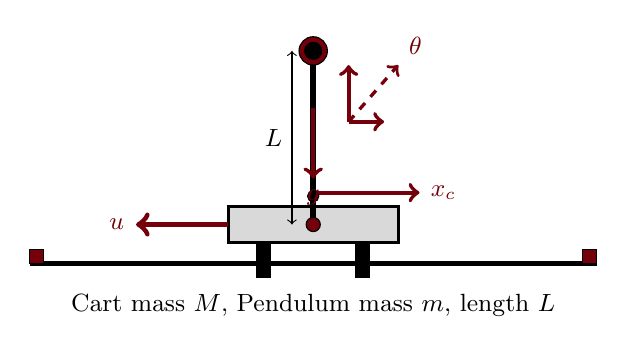
\begin{tikzpicture}[scale=0.9, every node/.style={font=\small}]
    % Define UofSC colors
    \definecolor{UofSCGarnet}{RGB}{115,0,10}
    \definecolor{UofSCBlack}{RGB}{0,0,0}

    % Ground
    \draw[line width=1.5pt, UofSCBlack] (-4, 0) -- (4, 0);
    \draw[fill=UofSCGarnet] (-4, 0) rectangle (-3.8, 0.2);
    \draw[fill=UofSCGarnet] (3.8, 0) rectangle (4, 0.2);

    % Cart
    \draw[fill=gray!30, draw=UofSCBlack, line width=1pt] (-1.2, 0.3) rectangle (1.2, 0.8);
    \draw[fill=UofSCBlack] (-0.8, 0.3) rectangle (-0.6, -0.2);
    \draw[fill=UofSCBlack] (0.6, 0.3) rectangle (0.8, -0.2);

    % Cart coordinate
    \draw[->, UofSCGarnet, line width=1.5pt] (0, 1) -- (1.5, 1) node[right] {$x_c$};
    \draw[fill=UofSCGarnet] (0, 0.95) circle (0.08);

    % Pendulum
    \draw[line width=2pt, UofSCBlack] (0, 0.55) -- (0, 3);
    \draw[fill=UofSCGarnet] (0, 3) circle (0.2);
    \draw[fill=UofSCGarnet] (0, 0.55) circle (0.1);

    % Pendulum angle
    \draw[->, UofSCGarnet, line width=1.5pt] (0.5, 2) -- (1, 2);
    \draw[->, UofSCGarnet, line width=1.5pt] (0.5, 2) -- (0.5, 2.8);
    \draw[->, UofSCGarnet, line width=1.2pt, dashed] (0.5, 2) -- (1.2, 2.8) node[above right] {$\theta$};

    % Mass center
    \draw[fill=UofSCBlack] (0, 3) circle (0.12);

    % Force arrow
    \draw[->, UofSCGarnet, line width=2pt] (-1.2, 0.55) -- (-2.5, 0.55) node[left] {$u$};

    % Length annotation
    \draw[<->, UofSCBlack] (-0.3, 0.55) -- (-0.3, 3) node[midway, left] {$L$};

    % Gravity arrow
    \draw[->, UofSCGarnet, line width=1.5pt] (0, 2.2) -- (0, 1.2) node[below] {$g$};

    % Labels
    \node[below] at (0, -0.3) {Cart mass $M$, Pendulum mass $m$, length $L$};
\end{tikzpicture}
\caption{Inverted pendulum on a cart system with coordinate definitions.}
\label{fig:inverted_pendulum_schematic}
\end{figure}

We begin by precisely defining the system configuration and coordinates. Consider a cart of mass $M$ that slides frictionlessly on a horizontal track. Attached to the cart at point $(x_c, 0)$ is a uniform rod of mass $m$ and length $L$ that pivots freely at the cart. The position of the cart along the track is denoted by $x_c(t)$, and the angle of the pendulum from the vertical upward direction is denoted by $\theta(t)$, where $\theta = 0$ corresponds to the perfectly upright (unstable) equilibrium. The cart is actuated by a horizontal force $u(t)$ applied by a motor, and this force is our control input. The goal of the control system is to determine $u(t)$ as a function of measured quantities such that the pendulum remains balanced near $\theta = 0$ even when subjected to disturbances.

To derive the equations of motion, we employ Lagrangian mechanics, a powerful framework that systematically accounts for energy transformations in mechanical systems. The Lagrangian $ \mathcal{L} $ is defined as the difference between the system's kinetic energy $T$ and potential energy $V$: $\mathcal{L} = T - V$. The equations of motion follow from the Euler-Lagrange equation $\frac{d}{dt}\left(\frac{\partial \mathcal{L}}{\partial \dot{q}_i}\right) - \frac{\partial \mathcal{L}}{\partial q_i} = Q_i$, where $q_i$ represents each generalized coordinate and $Q_i$ represents the generalized force associated with that coordinate.

Our system has two degrees of freedom, so we choose the generalized coordinates $q_1 = x_c$ (the cart position) and $q_2 = \theta$ (the pendulum angle). The first step in the Lagrangian approach is to express the kinetic and potential energies in terms of these coordinates and their time derivatives.

The cart moves purely in the horizontal direction, so its kinetic energy is simply $T_{\text{cart}} = \frac{1}{2}M\dot{x}_c^2$. The pendulum, however, has both translational and rotational kinetic energy. The center of mass of the pendulum is located at a distance $L/2$ from the pivot point. The coordinates of the pendulum's center of mass are given by the horizontal position $x_c + \frac{L}{2}\sin\theta$ and the vertical position $\frac{L}{2}\cos\theta$. Differentiating with respect to time, the velocity components of the pendulum center of mass are $\dot{x}_{\text{pend}} = \dot{x}_c + \frac{L}{2}\dot{\theta}\cos\theta$ in the horizontal direction and $\dot{y}_{\text{pend}} = -\frac{L}{2}\dot{\theta}\sin\theta$ in the vertical direction.

The translational kinetic energy of the pendulum is therefore $T_{\text{trans}} = \frac{1}{2}m\left(\dot{x}_{\text{pend}}^2 + \dot{y}_{\text{pend}}^2\right)$. Substituting the velocity expressions and simplifying, we obtain:
\begin{equation}
T_{\text{trans}} = \frac{1}{2}m\left[\left(\dot{x}_c + \frac{L}{2}\dot{\theta}\cos\theta\right)^2 + \left(-\frac{L}{2}\dot{\theta}\sin\theta\right)^2\right].
\end{equation}

Expanding this expression and collecting like terms:
\begin{equation}
T_{\text{trans}} = \frac{1}{2}m\left[\dot{x}_c^2 + L\dot{x}_c\dot{\theta}\cos\theta + \frac{L^2}{4}\dot{\theta}^2\cos^2\theta + \frac{L^2}{4}\dot{\theta}^2\sin^2\theta\right] = \frac{1}{2}m\left[\dot{x}_c^2 + L\dot{x}_c\dot{\theta}\cos\theta + \frac{L^2}{4}\dot{\theta}^2\right].
\end{equation}

The rotational kinetic energy of the pendulum about its center of mass is $T_{\text{rot}} = \frac{1}{2}I_{\text{cm}}\dot{\theta}^2$, where $I_{\text{cm}} = \frac{1}{12}mL^2$ is the moment of inertia of a uniform rod about its center. Thus $T_{\text{rot}} = \frac{1}{24}mL^2\dot{\theta}^2$.

Combining the translational and rotational contributions, the total kinetic energy of the pendulum is:
\begin{equation}
T_{\text{pend}} = \frac{1}{2}m\dot{x}_c^2 + \frac{1}{2}mL\dot{x}_c\dot{\theta}\cos\theta + \frac{1}{2}m\frac{L^2}{4}\dot{\theta}^2 + \frac{1}{24}mL^2\dot{\theta}^2 = \frac{1}{2}m\dot{x}_c^2 + \frac{1}{2}mL\dot{x}_c\dot{\theta}\cos\theta + \frac{7}{48}mL^2\dot{\theta}^2.
\end{equation}

The total kinetic energy of the entire system is the sum of the cart and pendulum kinetic energies:
\begin{equation}
T = T_{\text{cart}} + T_{\text{pend}} = \frac{1}{2}M\dot{x}_c^2 + \frac{1}{2}m\dot{x}_c^2 + \frac{1}{2}mL\dot{x}_c\dot{\theta}\cos\theta + \frac{7}{48}mL^2\dot{\theta}^2.
\end{equation}

Grouping terms, we write this in the compact form:
\begin{equation}
T = \frac{1}{2}(M + m)\dot{x}_c^2 + \frac{1}{2}mL\dot{x}_c\dot{\theta}\cos\theta + \frac{7}{48}mL^2\dot{\theta}^2.
\end{equation}

The potential energy of the system depends only on the vertical position of the pendulum's center of mass. Setting the zero of potential energy at the track level ($y = 0$), the potential energy is $V = mgy_{\text{pend}} = mg\left(\frac{L}{2}\cos\theta\right) = \frac{1}{2}mgL\cos\theta$. The cart has no potential energy since it moves horizontally at constant height.

We now have all the components needed to construct the Lagrangian:
\begin{equation}
\mathcal{L} = T - V = \frac{1}{2}(M + m)\dot{x}_c^2 + \frac{1}{2}mL\dot{x}_c\dot{\theta}\cos\theta + \frac{7}{48}mL^2\dot{\theta}^2 - \frac{1}{2}mgL\cos\theta.
\end{equation}

To derive the equations of motion, we apply the Euler-Lagrange equation for each generalized coordinate. We begin with the cart coordinate $x_c$. The partial derivatives are:
\begin{equation}
\frac{\partial \mathcal{L}}{\partial \dot{x}_c} = (M + m)\dot{x}_c + \frac{1}{2}mL\dot{\theta}\cos\theta,
\end{equation}
\begin{equation}
\frac{d}{dt}\left(\frac{\partial \mathcal{L}}{\partial \dot{x}_c}\right) = (M + m)\ddot{x}_c + \frac{1}{2}mL\ddot{\theta}\cos\theta - \frac{1}{2}mL\dot{\theta}^2\sin\theta,
\end{equation}
\begin{equation}
\frac{\partial \mathcal{L}}{\partial x_c} = 0.
\end{equation}

The generalized force associated with $x_c$ is the applied control force $u$, so $Q_{x_c} = u$. The Euler-Lagrange equation for $x_c$ is therefore:
\begin{equation}
(M + m)\ddot{x}_c + \frac{1}{2}mL\ddot{\theta}\cos\theta - \frac{1}{2}mL\dot{\theta}^2\sin\theta = u.
\end{equation}

This equation relates the cart acceleration to the pendulum dynamics through the coupling term involving $\ddot{\theta}$ and the centrifugal term involving $\dot{\theta}^2$. We will simplify this equation shortly after deriving the second equation.

For the pendulum coordinate $\theta$, the partial derivatives are:
\begin{equation}
\frac{\partial \mathcal{L}}{\partial \dot{\theta}} = \frac{1}{2}mL\dot{x}_c\cos\theta + \frac{7}{24}mL^2\dot{\theta},
\end{equation}
\begin{equation}
\frac{d}{dt}\left(\frac{\partial \mathcal{L}}{\partial \dot{\theta}}\right) = \frac{1}{2}mL\ddot{x}_c\cos\theta - \frac{1}{2}mL\dot{x}_c\dot{\theta}\sin\theta + \frac{7}{24}mL^2\ddot{\theta},
\end{equation}
\begin{equation}
\frac{\partial \mathcal{L}}{\partial \theta} = -\frac{1}{2}mL\dot{x}_c\dot{\theta}\sin\theta + \frac{1}{2}mgL\sin\theta.
\end{equation}

There are no explicit generalized forces applied to the pendulum angle (it is free to rotate on its pivot), so $Q_\theta = 0$. The Euler-Lagrange equation for $\theta$ gives:
\begin{equation}
\frac{1}{2}mL\ddot{x}_c\cos\theta - \frac{1}{2}mL\dot{x}_c\dot{\theta}\sin\theta + \frac{7}{24}mL^2\ddot{\theta} + \frac{1}{2}mL\dot{x}_c\dot{\theta}\sin\theta - \frac{1}{2}mgL\sin\theta = 0.
\end{equation}

Notice that the terms $-\frac{1}{2}mL\dot{x}_c\dot{\theta}\sin\theta$ and $+\frac{1}{2}mL\dot{x}_c\dot{\theta}\sin\theta$ cancel each other, simplifying the equation considerably:
\begin{equation}
\frac{1}{2}mL\ddot{x}_c\cos\theta + \frac{7}{24}mL^2\ddot{\theta} - \frac{1}{2}mgL\sin\theta = 0.
\end{equation}

We can multiply this entire equation by $2/(mL)$ to simplify the coefficients:
\begin{equation}
\ddot{x}_c\cos\theta + \frac{7}{12}L\ddot{\theta} - g\sin\theta = 0.
\end{equation}

We now have a system of two coupled second-order nonlinear differential equations:
\begin{equation}
(M + m)\ddot{x}_c + \frac{1}{2}mL\ddot{\theta}\cos\theta - \frac{1}{2}mL\dot{\theta}^2\sin\theta = u,
\end{equation}
\begin{equation}
\ddot{x}_c\cos\theta + \frac{7}{12}L\ddot{\theta} - g\sin\theta = 0.
\end{equation}

These equations fully describe the dynamics of the inverted pendulum on a cart. However, for control design purposes, we typically linearize these equations about the operating point of interest. For the inverted pendulum, the operating point is the unstable equilibrium at $\theta = 0$ (upright), $\dot{\theta} = 0$ (no rotation), and $\dot{x}_c = 0$ (cart stationary). At this operating point, $\sin\theta \approx \theta$, $\cos\theta \approx 1$, and terms involving $\dot{\theta}^2$ are second-order small quantities that we neglect.

Applying these approximations to the nonlinear equations, we obtain the linearized equations of motion:
\begin{equation}
(M + m)\ddot{x}_c + \frac{1}{2}mL\ddot{\theta} = u,
\end{equation}
\begin{equation}
\ddot{x}_c + \frac{7}{12}L\ddot{\theta} - g\theta = 0.
\end{equation}

These linear equations capture the essential dynamics of the inverted pendulum near the upright equilibrium and are much more amenable to analysis and control design than the original nonlinear equations.

To develop a state-space model, we first solve the linearized equations for the accelerations $\ddot{x}_c$ and $\ddot{\theta}$ in terms of the states and input. From the second equation, we have $\ddot{x}_c = - \frac{7}{12}L\ddot{\theta} + g\theta$. Substituting this into the first equation:
\begin{equation}
(M + m)\left(- \frac{7}{12}L\ddot{\theta} + g\theta\right) + \frac{1}{2}mL\ddot{\theta} = u.
\end{equation}

Expanding and collecting terms with $\ddot{\theta}$:
\begin{equation}
-\frac{7}{12}(M + m)L\ddot{\theta} + (M + m)g\theta + \frac{1}{2}mL\ddot{\theta} = u,
\end{equation}
\begin{equation}
\left[-\frac{7}{12}(M + m) + \frac{1}{2}m\right]L\ddot{\theta} + (M + m)g\theta = u.
\end{equation}

The coefficient of $\ddot{\theta}$ simplifies as follows:
\begin{equation}
-\frac{7}{12}(M + m) + \frac{1}{2}m = -\frac{7}{12}M - \frac{7}{12}m + \frac{6}{12}m = -\frac{7}{12}M - \frac{1}{12}m = -\frac{7M + m}{12}.
\end{equation}

Thus:
\begin{equation}
-\frac{7M + m}{12}L\ddot{\theta} + (M + m)g\theta = u.
\end{equation}

Solving for $\ddot{\theta}$:
\begin{equation}
\ddot{\theta} = \frac{12}{L(7M + m)}\left[(M + m)g\theta - u\right].
\end{equation}

We can also solve for $\ddot{x}_c$ by substituting this expression back into $\ddot{x}_c = - \frac{7}{12}L\ddot{\theta} + g\theta$:
\begin{equation}
\ddot{x}_c = - \frac{7}{12}L \cdot \frac{12}{L(7M + m)}\left[(M + m)g\theta - u\right] + g\theta = - \frac{7}{7M + m}\left[(M + m)g\theta - u\right] + g\theta.
\end{equation}

Simplifying:
\begin{equation}
\ddot{x}_c = -\frac{7(M + m)g\theta}{7M + m} + \frac{7u}{7M + m} + g\theta = \left[-\frac{7(M + m)}{7M + m} + 1\right]g\theta + \frac{7u}{7M + m}.
\end{equation}

The coefficient of $\theta$ simplifies as follows:
\begin{equation}
-\frac{7(M + m)}{7M + m} + 1 = -\frac{7M + 7m}{7M + m} + \frac{7M + m}{7M + m} = \frac{-7M - 7m + 7M + m}{7M + m} = \frac{-6m}{7M + m}.
\end{equation}

Therefore:
\begin{equation}
\ddot{x}_c = -\frac{6m}{7M + m}g\theta + \frac{7}{7M + m}u.
\end{equation}

Now we define the state vector for our system. Since we have two second-order equations, we need four state variables. A natural choice is:
\begin{equation}
\mathbf{x} = \begin{bmatrix} x_1 & x_2 & x_3 & x_4 \end{bmatrix}^T = \begin{bmatrix} x_c & \dot{x}_c & \theta & \dot{\theta} \end{bmatrix}^T.
\end{equation}

The state derivatives are:
\begin{equation}
\dot{x}_1 = \dot{x}_c = x_2,
\end{equation}
\begin{equation}
\dot{x}_2 = \ddot{x}_c = -\frac{6m}{7M + m}g x_3 + \frac{7}{7M + m}u,
\end{equation}
\begin{equation}
\dot{x}_3 = \dot{\theta} = x_4,
\end{equation}
\begin{equation}
\dot{x}_4 = \ddot{\theta} = \frac{12(M + m)g}{L(7M + m)} x_3 - \frac{12}{L(7M + m)}u.
\end{equation}

In standard state-space form $\dot{\mathbf{x}} = A\mathbf{x} + Bu$, the matrices are:
\begin{equation}
A = \begin{bmatrix}
0 & 1 & 0 & 0 \\
0 & 0 & -\frac{6mg}{7M + m} & 0 \\
0 & 0 & 0 & 1 \\
0 & 0 & \frac{12(M + m)g}{L(7M + m)} & 0
\end{bmatrix}, \quad
B = \begin{bmatrix} 0 \\ \frac{7}{7M + m} \\ 0 \\ -\frac{12}{L(7M + m)} \end{bmatrix}.
\end{equation}

If we choose the pendulum angle $\theta$ as the output (a common choice for balancing control), the output equation is $y = C\mathbf{x} + Du$ with:
\begin{equation}
C = \begin{bmatrix} 0 & 0 & 1 & 0 \end{bmatrix}, \quad D = \begin{bmatrix} 0 \end{bmatrix}.
\end{equation}

This state-space model reveals several important features of the inverted pendulum dynamics. First, notice that the matrix $A$ has a block structure that reflects the coupling between cart and pendulum dynamics. The bottom-right $2 \times 2$ block (rows and columns 3-4) captures the intrinsic dynamics of the pendulum, which we can analyze by considering the case where the cart is fixed ($\ddot{x}_c = 0$ and $\dot{x}_c = 0$). Setting $x_2 = 0$ and $u = 0$ in the state equations, the pendulum dynamics simplify to:
\begin{equation}
\begin{bmatrix} \dot{x}_3 \\ \dot{x}_4 \end{bmatrix} = \begin{bmatrix} 0 & 1 \\ \frac{12(M + m)g}{L(7M + m)} & 0 \end{bmatrix} \begin{bmatrix} x_3 \\ x_4 \end{bmatrix}.
\end{equation}

The eigenvalues of this $2 \times 2$ matrix are found from the characteristic equation:
\begin{equation}
\det\begin{bmatrix} -\lambda & 1 \\ \frac{12(M + m)g}{L(7M + m)} & -\lambda \end{bmatrix} = \lambda^2 - \frac{12(M + m)g}{L(7M + m)} = 0.
\end{equation}

Thus $\lambda = \pm \sqrt{\frac{12(M + m)g}{L(7M + m)}}$. For a typical inverted pendulum with $M \gg m$, this simplifies to $\lambda \approx \pm \sqrt{\frac{12g}{7L}}$. The positive eigenvalue indicates that the upright equilibrium is exponentially unstable, meaning any small deviation from vertical will grow exponentially over time. This is the fundamental challenge of the inverted pendulum: without control action, the system naturally diverges from the desired operating point.

The full $4 \times 4$ system matrix has eigenvalues that can be determined by solving the characteristic equation $\det(sI - A) = 0$. Computing this determinant:
\begin{equation}
\det\begin{bmatrix}
s & -1 & 0 & 0 \\
0 & s & \frac{6mg}{7M + m} & 0 \\
0 & 0 & s & -1 \\
0 & 0 & -\frac{12(M + m)g}{L(7M + m)} & s
\end{bmatrix} = s^2 \left[s^2 - \frac{12(M + m)g}{L(7M + m)}\right] - \frac{6mg}{7M + m} \cdot \frac{12(M + m)g}{L(7M + m)} s.
\end{equation}

After simplification, the characteristic equation is:
\begin{equation}
s\left[s^3 - \frac{12(M + m)g}{L(7M + m)}s - \frac{72mg}{L(7M + m)^2}\right] = 0.
\end{equation}

One eigenvalue is always at $s = 0$, corresponding to the cart position $x_c$ being an unobservable mode (we can add or subtract a constant from $x_c$ without affecting the dynamics). The remaining cubic equation has two unstable roots (positive real parts) and one stable root (negative real part). The presence of unstable poles means the open-loop system is not stabilizable by simply letting go—the pendulum will fall, and the cart will respond to the coupling in ways that cannot counteract the instability.

The control design problem for the inverted pendulum is now clear: we must design a feedback controller that shifts all poles of the system to the left half-plane (negative real parts), thereby stabilizing the inherently unstable equilibrium. This is achievable through state feedback, where we measure all four states (or estimate them from available measurements) and compute the control input as a linear combination:
\begin{equation}
u = -K_1 x_c - K_2 \dot{x}_c - K_3 \theta - K_4 \dot{\theta}.
\end{equation}

The gains $K_1, K_2, K_3, K_4$ are chosen such that the closed-loop system matrix $A - BK$ has all eigenvalues with negative real parts. This is the pole placement problem we will address in detail in later chapters.

\begin{example}{Linearized Inverted Pendulum Dynamics — Numerical Illustration}
Consider an inverted pendulum with the following physical parameters: cart mass $M = 1$ kg, pendulum mass $m = 0.2$ kg, pendulum length $L = 0.5$ m, and gravitational acceleration $g = 9.81$ m/s². Substituting these values into our linearized model, we first compute the coefficients.

The denominator appearing throughout our equations is $7M + m = 7(1) + 0.2 = 7.2$ kg. The state-space matrices become:
\begin{equation}
A = \begin{bmatrix}
0 & 1 & 0 & 0 \\
0 & 0 & -9.81 & 0 \\
0 & 0 & 0 & 1 \\
0 & 0 & 49.05 & 0
\end{bmatrix}, \quad
B = \begin{bmatrix} 0 \\ 0.9722 \\ 0 \\ -3.333 \end{bmatrix}.
\end{equation}

Computing the eigenvalues of the open-loop $A$ matrix, we find $\lambda = 0$, $\lambda = -7.00$, and $\lambda = \pm 7.00$. The pair of purely imaginary eigenvalues at $\pm 7.00$ (in this simplified case where $M \gg m$) indicates marginal instability—if the pendulum tips, it will oscillate with increasing amplitude. The zero eigenvalue corresponds to the fact that the absolute cart position doesn't affect the dynamics; only relative motion matters.

If we design a state feedback controller with gains $K = \begin{bmatrix} -1.5 & -4.0 & -60.0 & -10.0 \end{bmatrix}$, the closed-loop system has eigenvalues at approximately $\lambda = -2.0$, $\lambda = -3.0$, and $\lambda = -5.0 \pm 2.5j$. All eigenvalues have negative real parts, confirming that the closed-loop system is stable. The gains can be interpreted physically: $K_3 = -60$ provides strong feedback proportional to the pendulum angle (correct more aggressively for larger deviations from vertical), $K_4 = -10$ provides damping proportional to angular velocity (resist rapid swinging motion), and the cart-related gains help maintain the cart near some reference position while managing the coupling between the two degrees of freedom.
\end{example}

The inverted pendulum illustrates several fundamental principles that recur throughout control systems engineering. First, accurate mathematical modeling is not optional—it is essential. The coupling between cart and pendulum dynamics means that a controller designed for a simplified model (ignoring the cart dynamics, for instance) will fail dramatically when applied to the actual system. Second, unstable systems require feedback for stabilization; no amount of open-loop planning can maintain an unstable equilibrium in the presence of disturbances. Third, the pole placement approach (choosing desired closed-loop dynamics and computing the required feedback gains) provides a systematic framework for control design, rather than relying on trial and error.

The inverted pendulum also serves as a benchmark problem for testing control algorithms. Its apparent simplicity (just two degrees of freedom, one input) belies the depth of analysis required to understand and control it. Variations of this problem—inverted pendulum on a moving cart, double inverted pendulum, inverted pendulum with time delays or nonlinear friction—continue to be active areas of research and serve as stepping stones to more complex real-world control challenges such as rocket launch vehicle stabilization, humanoid robot balance, and spacecraft attitude control.


\subsection{Case Study 3 --- Thermal System with Multiple Zones}
\label{sec:case_thermal}

\subsection{Case Study 3 --- Thermal System with Multiple Zones}

Many practical thermal systems involve heat transfer across multiple interconnected regions. Consider a building with several rooms, a semiconductor wafer processing tool with multiple temperature zones, or an industrial furnace with different thermal regions. In each case, we must understand how heat flows between zones and how we can model these interactions for control purposes. This case study develops a comprehensive model of a multi-zone thermal system, introduces the concept of state-space representation for distributed-parameter systems, and demonstrates how physical insight can guide model reduction and controller design.

The physical phenomena governing multi-zone thermal systems are straightforward extensions of the single-zone case we examined in Section 1.8.1. Each zone possesses thermal mass, meaning it can store energy in proportion to its temperature. Heat transfers between adjacent zones through conduction, following Fourier's law, which states that the heat flow rate is proportional to the temperature difference and the thermal conductivity of the material separating the zones. Each zone also exchanges heat with its surroundings through convection, where the rate of heat loss to the environment depends on the temperature difference between the zone and ambient conditions, scaled by a convective heat transfer coefficient and the surface area exposed to the environment. Additionally, heating elements within each zone can inject thermal energy, providing the control inputs we manipulate to regulate temperatures.

To develop a mathematical model, we apply the principle of energy conservation to each thermal zone. The net rate of energy accumulation within a zone equals the sum of all energy inflows minus the sum of all energy outflows. For a zone labeled $i$ with temperature $T_i$, the rate of energy accumulation is given by $C_i \dot{T}_i$, where $C_i$ represents the thermal capacitance of the zone and the dot denotes differentiation with respect to time. This capacitance depends on the mass of material in the zone, its specific heat capacity, and any additional thermal mass from equipment or furnishings within the zone. The thermal capacitance has units of joules per degree Celsius, or equivalently, watt-seconds per degree Celsius, reflecting the energy required to raise the zone temperature by one degree.

The energy flows entering and leaving zone $i$ arise from three distinct mechanisms. First, conductive heat transfer from each adjacent zone $j$ occurs at a rate $k_{ij}(T_j - T_i)$, where $k_{ij}$ is the thermal conductance between zones $i$ and $j$. The thermal conductance depends on the thermal conductivity of the separating material, the cross-sectional area available for heat transfer, and the path length over which conduction occurs. Note that this expression naturally captures the direction of heat flow: if $T_j > T_i$, heat flows from zone $j$ to zone $i$, adding energy to zone $i$. Second, convective heat loss to the environment occurs at a rate $h_{i}(T_i - T_{\text{amb}})$, where $h_i$ is the overall convective heat transfer coefficient for zone $i$ and $T_{\text{amb}}$ represents the ambient or outdoor temperature. This coefficient accounts for all heat transfer from the zone's exposed surfaces to the surrounding air, including effects from natural convection, radiation, and any air infiltration. Third, heating inputs from HVAC systems, electric heaters, or other sources inject energy at rates $u_i$, which serve as our control inputs. Combining these contributions, the energy balance equation for zone $i$ becomes:

$$C_i \dot{T}_i = \sum_{j \in \mathcal{N}_i} k_{ij}(T_j - T_i) + h_i(T_{\text{amb}} - T_i) + u_i$$

where $\mathcal{N}_i$ denotes the set of zones adjacent to zone $i$. This equation captures the complete dynamics of how temperature in each zone evolves based on interactions with neighboring zones, environmental losses, and active heating.

Let us illustrate these concepts with a concrete example involving three thermally interconnected zones arranged in a linear configuration, as might occur in a simple building with three rooms connected in sequence. Suppose zone 1 represents an exterior room with significant exposure to outdoor conditions, zone 2 is an interior hallway serving as a buffer zone, and zone 3 is another exterior room on the opposite side of the building. The thermal capacitances are $C_1 = 5000$ J/$\!^\circ$C, $C_2 = 3000$ J/$\!^\circ$C, and $C_3 = 5000$ J/$\!^\circ$C. The conductive coupling between zones 1 and 2 has conductance $k_{12} = 20$ W/$\!^\circ$C, while the coupling between zones 2 and 3 has the same conductance $k_{23} = 20$ W/$\!^\circ$C. Zone 1 loses heat to the environment with coefficient $h_1 = 15$ W/$\!^\circ$C, zone 2 has minimal exposure with $h_2 = 5$ W/$\!^\circ$C, and zone 3 loses heat with $h_3 = 15$ W/$\!^\circ$C. The ambient temperature is $T_{\text{amb}} = 5^\circ$C, representing a cold winter day. Each zone has an independent heating input: $u_1$, $u_2$, and $u_3$ in watts.

Applying the energy balance equation to each zone yields a system of three coupled first-order differential equations:

\begin{align}
\dot{T}_1 &= \frac{k_{12}}{C_1}(T_2 - T_1) + \frac{h_1}{C_1}(T_{\text{amb}} - T_1) + \frac{u_1}{C_1} \\
\dot{T}_2 &= \frac{k_{12}}{C_2}(T_1 - T_2) + \frac{k_{23}}{C_2}(T_3 - T_2) + \frac{h_2}{C_2}(T_{\text{amb}} - T_2) + \frac{u_2}{C_2} \\
\dot{T}_3 &= \frac{k_{23}}{C_2}(T_2 - T_3) + \frac{h_3}{C_3}(T_{\text{amb}} - T_3) + \frac{u_3}{C_3}
\end{align}

Substituting the numerical values, we obtain:

\begin{align}
\dot{T}_1 &= 0.004(T_2 - T_1) + 0.003(5 - T_1) + \frac{u_1}{5000} \\
\dot{T}_2 &= \frac{20}{3000}(T_1 - T_2) + \frac{20}{3000}(T_3 - T_2) + \frac{5}{3000}(5 - T_2) + \frac{u_2}{3000} \\
\dot{T}_3 &= \frac{20}{5000}(T_2 - T_3) + 0.003(5 - T_3) + \frac{u_3}{5000}
\end{align}

Simplifying the coefficients:

\begin{align}
\dot{T}_1 &= 0.004T_2 - 0.007T_1 + 0.015 + \frac{u_1}{5000} \\
\dot{T}_2 &= 0.00667T_1 + 0.00667T_3 - 0.0193T_2 + 0.00833 + \frac{u_2}{3000} \\
\dot{T}_3 &= 0.004T_2 - 0.007T_3 + 0.015 + \frac{u_3}{5000}
\end{align}

This system of differential equations describes how the three zone temperatures evolve over time given heating inputs and environmental conditions. The constant terms arising from the ambient temperature represent heat loss or gain from the environment even when zone temperatures are zero, serving as a constant disturbance to the system.

The state-space representation provides a compact and powerful framework for analyzing such multi-input multi-output systems. We define the state vector as $\mathbf{x} = \begin{bmatrix} T_1 & T_2 & T_3 \end{bmatrix}^T$, the input vector as $\mathbf{u} = \begin{bmatrix} u_1 & u_2 & u_3 \end{bmatrix}^T$, and the output vector as $\mathbf{y} = \mathbf{x}$ if we measure all zone temperatures. The system dynamics take the standard linear form $\dot{\mathbf{x}} = A\mathbf{x} + B\mathbf{u} + \mathbf{d}$, where $A$ is the state matrix capturing internal couplings, $B$ is the input matrix mapping heating rates to temperature derivatives, and $\mathbf{d}$ represents the constant disturbance from ambient conditions. For our three-zone example, these matrices are:

$$A = \begin{bmatrix}
-0.007 & 0.004 & 0 \\
0.00667 & -0.0193 & 0.00667 \\
0 & 0.004 & -0007
\end{bmatrix}, \quad
B = \begin{bmatrix}
\frac{1}{5000} & 0 & 0 \\
0 & \frac{1}{3000} & 0 \\
0 & 0 & \frac{1}{5000}
\end{bmatrix}, \quad
\mathbf{d} = \begin{bmatrix}
0.015 \\ 0.00833 \\ 0.015
\end{bmatrix}$$

This representation makes the structure of the system immediately apparent. The diagonal entries of $A$ are negative, indicating that each zone's temperature tends to decrease when isolated from other zones, reflecting the inherent heat losses to the environment. The off-diagonal entries are positive, showing that increasing a neighbor's temperature tends to increase the local temperature through conductive heat transfer. The input matrix $B$ is diagonal, meaning each heating input affects only its own zone temperature directly, though indirect effects propagate through the coupling terms in $A$.

An important concept in multi-zone thermal systems is time-scale separation, which arises when different parts of the system respond at vastly different speeds. In our example, the two exterior zones (1 and 3) have larger thermal capacitances ($5000$ J/$\!^\circ$C) and significant environmental exposure, while the interior hallway zone (2) has smaller thermal capacitance ($3000$ J/$\!^\circ$C) and minimal environmental losses. This configuration creates two distinct time scales: the interior zone responds relatively quickly to changes in neighboring temperatures because its small thermal capacitance means it requires less energy to change temperature, while the exterior zones respond more slowly due to their larger thermal masses and the continuous energy drain of environmental heat loss.

To analyze time-scale separation quantitatively, we examine the eigenvalues of the state matrix $A$. These eigenvalues, which are the roots of the characteristic equation $\det(sI - A) = 0$, determine the natural response rates of the system. For our three-zone system, computing the eigenvalues yields approximately $s_1 = -0.025$ rad/s, $s_2 = -0.011$ rad/s, and $s_3 = -0.005$ rad/s. The corresponding time constants are $\tau_i = -1/s_i$, giving $\tau_1 \approx 40$ s, $\tau_2 \approx 90$ s, and $\tau_3 \approx 200$ s. The ratio between the slowest and fastest time constants is about 5:1, representing moderate time-scale separation. In more extreme cases, such as a building with massive thermal mass in walls and floors but rapid air temperature response, this ratio might exceed 100:1, creating strongly separated dynamics.

Time-scale separation has profound implications for control system design. When dynamics occur on significantly different time scales, we can often design controllers that treat the slow and fast dynamics somewhat independently. The fast dynamics might be controlled using aggressive feedback that responds quickly to disturbances, while the slow dynamics might use more gradual control actions that avoid exciting the faster modes unnecessarily. This separation is particularly valuable in building HVAC systems, where the fast dynamics of zone air temperatures can be controlled independently of the slow dynamics of thermal mass in walls and furniture, allowing for efficient hierarchical control architectures.

Model reduction techniques leverage time-scale separation and other structural properties to obtain simpler models that capture the essential behavior of the original system. In a multi-zone thermal system, we might reduce the model order by identifying zones with similar temperatures that can be lumped together, by neglecting high-frequency modes that have minimal impact on the system's low-frequency behavior, or by identifying dominant state variables that capture most of the system's energy. The reduced-order model provides a computationally tractable representation for controller design while preserving the dynamic characteristics most important for achieving control objectives.

One common reduction approach for thermal systems is modal truncation, where we retain only the slowest modes of the system and discard faster modes that contribute little to the overall response. For our three-zone example, if we retained only the slowest mode corresponding to $s_3 = -0.005$ rad/s, we would obtain a first-order model that captures the long-term thermal behavior of the entire building but misses the faster transient responses in individual zones. This reduced model might be suitable for supervisory control that sets setpoints for zone-level controllers, but would be inadequate for direct zone temperature regulation. The trade-off between model fidelity and complexity always involves understanding which aspects of system behavior matter for the intended control objective.

Spatially lumped approximations transform distributed-parameter systems, where temperature varies continuously in space, into finite-dimensional state-space models with discrete state variables representing temperatures at specific locations. This approach divides the distributed system into zones or nodes, assumes uniform temperature within each zone, and derives lumped energy balance equations as we have done. The accuracy of the lumped approximation depends on how well the uniform-temperature assumption holds, which in turn depends on the thermal diffusivity of the material and the characteristic length scale of each zone. Materials with high thermal diffusivity conduct heat rapidly, making temperature more uniform across the zone and justifying the lumped approximation. Materials with low thermal diffusivity develop significant temperature gradients within the zone, requiring smaller zones or more sophisticated distributed models.

The choice of zone boundaries in a lumped approximation involves physical insight and engineering judgment. Consider a building wall consisting of insulation, sheathing, and drywall. Rather than modeling each layer as a separate zone, we might combine all wall layers into a single thermal mass representing the wall's total thermal capacitance. The heat transfer through the wall would then be modeled as conduction from the interior air zone to the exterior air zone through an effective thermal resistance representing the combined resistance of all wall layers. This approach reduces model complexity while preserving the essential energy storage and transfer dynamics, provided we correctly calculate the equivalent thermal capacitance and conductance from the layer properties.

To illustrate model reduction through lumping, suppose we decide that zones 1 and 3 in our three-zone example are thermally similar and strongly coupled to the environment, while zone 2 acts primarily as a thermal buffer between them. We might create a reduced two-zone model by lumping zones 1 and 3 into a single "exterior zone" with combined thermal capacitance $C_e = C_1 + C_3 = 10000$ J/$\!^\circ$C and effective environmental conductance $h_e = h_1 + h_3 = 30$ W/$\!^\circ$C. The interior zone remains unchanged with $C_i = 3000$ J/$\!^\circ$C and $h_i = 5$ W/$\!^\circ$C. The coupling between the lumped exterior zone and the interior zone becomes $k_{ei} = k_{12} + k_{23} = 40$ W/$\!^\circ$C, representing the combined conductive paths through both original interfaces. The reduced two-zone model is:

\begin{align}
\dot{T}_e &= \frac{k_{ei}}{C_e}(T_i - T_e) + \frac{h_e}{C_e}(T_{\text{amb}} - T_e) + \frac{u_1 + u_3}{C_e} \\
\dot{T}_i &= \frac{k_{ei}}{C_e}(T_e - T_i) + \frac{h_i}{C_i}(T_{\text{amb}} - T_i) + \frac{u_2}{C_i}
\end{align}

Substituting values:

\begin{align}
\dot{T}_e &= 0.004(T_i - T_e) + 0.003(5 - T_e) + \frac{u_1 + u_3}{10000} \\
\dot{T}_i &= 0.0133(T_e - T_i) + 0.00167(5 - T_i) + \frac{u_2}{3000}
\end{align}

This reduced model captures the essential dynamics of the original three-zone system with approximately half the state dimension, making controller design simpler while preserving the key interactions between interior and exterior thermal behavior.

The multi-zone thermal system studied in this case study exemplifies several recurring themes in control systems engineering. First, physical principles from thermodynamics and heat transfer provide the foundation for deriving accurate models from first principles. Second, the state-space representation offers a unified framework for analyzing systems with multiple inputs, outputs, and internal couplings. Third, time-scale separation, when present, creates opportunities for hierarchical control architectures and model reduction. Fourth, lumped approximations transform distributed systems into tractable finite-dimensional models, with accuracy depending on the validity of the uniform-temperature assumption within each zone. These concepts extend far beyond thermal systems to mechanical, electrical, chemical, and biological systems throughout engineering and science.

\begin{table}[htbp]
\centering
\begin{tabular}{|l|c|c|c|}
\hline
\rowcolor{UofSCGarnet}
\textcolor{white}{\textbf{Parameter}} & \textcolor{white}{\textbf{Zone 1}} & \textcolor{white}{\textbf{Zone 2}} & \textcolor{white}{\textbf{Zone 3}} \\
\hline
Thermal Capacitance $C_i$ (J/$\!^\circ$C) & 5000 & 3000 & 5000 \\
\hline
Environmental Conductance $h_i$ (W/$\!^\circ$C) & 15 & 5 & 15 \\
\hline
Coupling to Zone 2 $k_{i2}$ (W/$\!^\circ$C) & 20 & 20 & 20 \\
\hline
Initial Temperature $T_i(0)$ ($\!^\circ$C) & 10 & 15 & 10 \\
\hline
Heating Input $u_i$ (W) & $u_1$ & $u_2$ & $u_3$ \\
\hline
\end{tabular}
\captionsetup{type=table}
\caption{Parameters for the three-zone thermal system example. The thermal capacitances represent the energy storage capacity of each zone. Environmental conductances capture heat loss to ambient conditions. Coupling conductances represent conductive heat transfer between adjacent zones.}
\end{table}


%-------------------------------------------------------------------------------
% SECTION 1.9: SUMMARY
%-------------------------------------------------------------------------------
\section{Chapter Summary and Bridge to Control Design}
\label{sec:chapter_summary}

\subsection{Key Concepts and Takeaways}
\label{sec:key_concepts}

\subsection{1.9.1 Key Concepts and Takeaways}

This section synthesizes the fundamental concepts presented throughout Chapter 1, providing a unified perspective on the systematic approach to modeling dynamic systems that will serve as the foundation for analysis and design in subsequent chapters. The overarching theme that emerges from our examination of mechanical, electrical, thermal, and fluid systems is the deep connection between physical phenomena and their mathematical descriptions---understanding one illuminates the other, and proficiency in control systems requires fluency in both domains.

The modeling workflow introduced in this chapter follows a sequential progression that mirrors the natural process of understanding and describing physical systems. The first stage, physical analysis, requires the engineer to identify energy storage elements, recognize energy dissipation mechanisms, and trace the pathways through which energy flows within the system. This physical intuition is not merely a preliminary step but rather provides the conceptual scaffolding upon which all subsequent mathematical work rests. When we identify a mass in a mechanical system or an inductance in an electrical circuit, we are recognizing a capacity for energy storage that will manifest as a dynamical element in our equations. Similarly, identifying resistors, dampers, or friction elements directs our attention to the mechanisms through which system energy is gradually converted to heat and lost from the system.

Mathematical formulation transforms the physical understanding into precise algebraic and differential relationships. The fundamental physical laws---Newton's laws for mechanical systems, Kirchhoff's laws for electrical systems, and their analogues in thermal and fluid domains---provide the governing equations that relate system variables to one another. The resulting ordinary differential equations capture the cause-and-effect structure of the system: the left-hand side typically represents the system's inertial or capacitive response, while the right-hand side represents the forcing functions and dissipative effects. The structure of these equations, particularly the order of differentiation and the presence or absence of coupling terms, directly reflects the underlying physics. A second-order differential equation with constant coefficients, for instance, immediately suggests a system with one independent energy storage element of each type, subject to linear dissipation.

Linearization represents a critical technique for extending the applicability of powerful linear analysis methods to systems that may exhibit nonlinear behavior over their full operating range. By restricting our attention to small perturbations about an equilibrium point, we can approximate nonlinear functions with their first-order Taylor series expansions, yielding linear differential equations that accurately describe local system behavior. This process preserves the essential structure of the dynamics while enabling the full arsenal of frequency response, root locus, and state-space techniques developed in control theory. The Jacobian matrices that arise in linearization connect directly to the state-space representation, as discussed in Section 1.6, providing a natural bridge between local linear analysis and global system description.

The conversion between mathematical representations completes the modeling workflow by enabling different analytical approaches to the same underlying system. Table 1.1 summarizes the key equivalences and trade-offs among the three primary representations.

\begin{table}[htbp]
\centering
\begin{tabular}{|p{0.22\textwidth}|p{0.22\textwidth}|p{0.22\textwidth}|p{0.22\textwidth}|}
\hline
\textbf{Characteristic} & \textbf{ODE Form} & \textbf{Transfer Function} & \textbf{State Space} \\
\hline
Input-output structure & Implicit in higher-order equation & Explicit $Y(s)/U(s)$ relationship & Requires output equation \\
\hline
Initial conditions & Naturally incorporated & Must be zero for standard form & Explicitly included in state vector \\
\hline
Multi-input multi-output & Cumbersome & Does not extend directly & Natural representation \\
\hline
Physical insight & Direct connection to physics & Frequency domain intuition & Energy-based interpretation \\
\hline
System order & Determined by highest derivative & Degree of denominator polynomial & Dimension of state vector \\
\hline
\end{tabular}
\\[0.5em]
\textcolor{UofSCGarnet}{\textbf{Table 1.1}} Comparison of mathematical representations for linear time-invariant systems.
\end{table}

Several recurring themes weave through our examination of diverse physical systems, revealing fundamental unity beneath surface differences. The concept of analogous systems proves particularly powerful: mechanical translational systems can be mapped to electrical circuits through force-current or force-voltage analogies, and these analogies extend to thermal and fluid domains as well. When we recognize that a mechanical mass experiencing damping is governed by equations identical in form to those describing an RL circuit, we gain the ability to transfer intuitions developed in one domain to problems in another. This analogy-based reasoning accelerates physical understanding and prevents the duplication of analytical effort.

Energy serves as the unifying concept across all physical domains. In mechanical systems, kinetic energy resides in moving masses while potential energy is stored in springs and gravitational fields. In electrical systems, magnetic fields store energy in inductances while electric fields store energy in capacitors. Thermal systems store energy in the internal energy of materials, and fluid systems store energy through compression in pneumatic systems or elevation in hydraulic systems. The rate of energy transfer across system boundaries appears as power, and the derivative of stored energy with respect to time equals the net power flow into each storage element. This energy perspective provides a powerful check on mathematical models: physically reasonable models must satisfy energy conservation principles, and discrepancies between computed energy flows often reveal errors in formulation.

The state-space representation, while mathematically equivalent to the other forms, offers unique conceptual and practical advantages that merit special emphasis. The state vector captures all information needed to predict future system behavior given current inputs, and each state variable typically corresponds to an energy storage element in the physical system. This correspondence enables the physical interpretation of state trajectories: the evolution of state variables through the state space represents the flow of energy through storage elements and its gradual dissipation through resistive elements. The matrix structures $A$, $B$, $C$, and $D$ encode the complete dynamics, with $A$ governing unforced behavior and $B$ describing how inputs affect the state derivatives. Understanding the physical meaning of these matrices reinforces the connection between mathematical abstraction and physical reality.

Model validation closes the modeling loop by ensuring that our mathematical descriptions adequately represent the physical systems they model. This validation process involves comparing predicted responses to measured responses from the actual system, identifying discrepancies, and iteratively refining the model until acceptable accuracy is achieved. The validation stage reminds us that mathematical models are tools created to serve engineering purposes, not ends in themselves, and that even elegant mathematical derivations must ultimately answer to physical reality.

The conceptual framework developed in this chapter---physical analysis, mathematical formulation, linearization, representation conversion, and validation---provides a template applicable to every control system problem encountered in this textbook. As we progress to system analysis, controller design, and implementation in subsequent chapters, the foundational understanding of system modeling will enable deeper insights and more effective engineering decisions. The investment in thoroughly understanding modeling pays dividends throughout the study of control systems.

\subsection{How Modeling Choices Affect Control Design}
\label{sec:modeling_choices}

\subsection{How Modeling Choices Affect Control Design}

The control design process does not begin with a blank slate. Every decision made during the modeling phase—whether explicit or implicit—propagates forward and constrains what controllers can ultimately be designed and how well they will perform. Understanding this relationship between modeling and control design is essential for developing an intuition that will serve the control engineer throughout this textbook and in professional practice. The choices made in constructing a mathematical model determine not only which analysis tools are applicable but also which design methods will yield feasible solutions and what performance limits will be encountered.

The decision to linearize a nonlinear model around an operating point fundamentally shapes the control design landscape. Linearized models of the form $\dot{x} = Ax + Bu$ and $y = Cx + Du$ open the door to both classical frequency-domain design techniques and modern state-space methods, but this accessibility comes with important implications. Classical design approaches, which we explore in Chapters 6 through 9, rely on transfer function representations and frequency concepts such as B responseode plots, Nyquist criteria, and gain and phase margins. These tools provide deep intuition about stability and performance but require models that capture the essential input-output dynamics while remaining amenable to frequency-domain analysis. State-space design methods, covered in Chapters 10 through 13, leverage the internal description captured in the matrices $(A, B, C, D)$ to employ techniques including pole placement, linear quadratic regulators, and observers. A linearized model provides the foundation for both design paradigms, allowing the control engineer to select the approach best suited to the specific application requirements.

Model accuracy requirements are not universal but rather depend intimately on the performance specifications and robustness margins demanded by the application. A model developed for a cruise control system with modest performance requirements can tolerate significant approximation error, while a precision positioning system for a semiconductor manufacturing tool demands accurate representation of dynamics across a wide frequency range. This relationship between model fidelity and design requirements creates a design trade-off that must be navigated carefully. If the model underrepresents the true system dynamics, the designed controller may fail to achieve specifications or, worse, may introduce instability when deployed on the actual hardware. Conversely, excessive model accuracy demands can make the design process unnecessarily complex without corresponding benefits. The robustness margins discussed in Chapter 8—gain margin, phase margin, and sensitivity functions—provide the theoretical framework for understanding how much model uncertainty can be tolerated and, equivalently, how accurate the model must be to achieve reliable performance.

The structural properties of a model—its relative degree, zeros, and pole locations—determine the fundamental limits of achievable performance in ways that no amount of controller sophistication can overcome. The relative degree, defined as the difference between the number of poles and zeros in the transfer function, dictates the earliest time at which a control action can influence the output. A system with relative degree $n$ requires at least $n$ time constants before the output responds to an input change, establishing a fundamental speed limitation that affects every subsequent design decision. Zeros in the transfer function create directions in which the system cannot be controlled, limiting the achievable closed-loop pole locations and constraining the bandwidth attainable in certain frequency ranges. Chapter 5 develops these fundamental limitations rigorously, showing that control design is not merely about selecting arbitrary closed-loop behaviors but about working within the constraints imposed by the system's inherent dynamics. Pole locations in the open-loop model similarly constrain achievable closed-loop behavior through the region of the complex plane from which the controller cannot escape due to the inherent dynamics of the physical system.

The choice between different mathematical representations—transfer functions versus state-space models, continuous-time versus discrete-time formulations, input-output models versus input-state-output models—affects not only which analysis tools are available but also what controller structures can be feasibly implemented. A transfer function representation naturally suggests controllers described by rational functions, while a state-space model enables dynamic feedback laws with internal state dynamics. The transition to digital control systems, explored in Chapter 7, requires discretized models that preserve the essential characteristics of the continuous-time system while enabling implementation on digital processors. This representation choice has practical consequences: certain controller structures that appear natural in one representation may require awkward approximation or transformation in another, potentially introducing design errors or implementation complications. Understanding these representation effects allows the engineer to select modeling approaches that facilitate the eventual controller implementation.

The connection between modeling decisions and control design possibilities becomes clearer when examined through specific properties and their implications. The following table summarizes how key modeling choices propagate through the design process.

\begin{table}[h!]
\centering
\begin{tabular}{|p{2.0in}|p{2.5in}|p{2.0in}|}
\hline
\textbf{Modeling Decision} & \textbf{Enables} & \textbf{Constrains} \\
\hline
Linearization about operating point & Frequency-domain design, state-space methods & Valid only near operating point, cannot capture large-signal behavior \\
\hline
Model order reduction & Simplified analysis and design & May remove dynamics relevant for performance or stability \\
\hline
Neglecting higher-order dynamics & Tractable controller complexity & Fundamental bandwidth limitation, potential instability at high frequencies \\
\hline
Ignoring nonlinearities & Linear design techniques & Cannot predict limit cycles, saturation effects, or bifurcations \\
\hline
Discrete-time approximation & Digital implementation & Aliasing effects, sampling-induced stability margins \\
\hline
\end{tabular}
\\
\vskip 0.15in
\hskip 0.5in\begin{tabular}{|p{2.0in}|p{2.5in}|p{2.0in}|}
\hline
\textbf{Model Property} & \textbf{Design Implication} & \textbf{Affected Chapters} \\
\hline
Relative degree & Minimum achievable settling time & Chapters 4, 5, 8 \\
\hline
Zero locations & Achievable bandwidth, peak overshoot limits & Chapters 5, 6, 9 \\
\hline
Pole locations & Open-loop stability, natural response characteristics & Chapters 3, 4, 10 \\
\hline
Controllability and observability & Feasibility of state feedback and observer design & Chapters 10, 11, 12 \\
\hline
Minimum phase property & Achievable tracking performance & Chapters 6, 9, 13 \\
\hline
\end{tabular}
\vskip 0.1in
\end{table}

The design chapters that follow this one assume familiarity with the modeling concepts developed in Chapters 2 and 3. Chapter 4 establishes the fundamental limitations imposed by physical systems, providing the theoretical foundation for understanding why certain control objectives are achievable while others are not. Chapters 5 through 9 develop classical and frequency-domain design methods, relying on transfer function representations derived from linearized models. Chapters 10 through 13 present modern state-space approaches, leveraging the internal description provided by state-space models to achieve more sophisticated performance objectives. Throughout these chapters, the connection between modeling assumptions and design possibilities remains central—each new design method builds upon the modeling foundation laid in earlier chapters, and each method inherits the limitations and opportunities created by those initial modeling choices.

The effective control engineer develops the ability to work backward from design requirements to modeling decisions, understanding which aspects of system behavior must be captured accurately and which can be approximated or neglected. This bidirectional understanding—knowing both how models constrain design and how design requirements drive modeling decisions—distinguishes the practitioner who produces robust, implementable controllers from one who produces mathematically correct but practically infeasible solutions. As you progress through the design chapters, return frequently to the modeling foundations established here, and consider how the choices made in representing a physical system continue to shape every subsequent design decision.


\subsection{Preview of Advanced Topics and Further Study}
\label{sec:advanced_topics}

\subsection{Preview of Advanced Topics and Further Study}

The methods developed in this chapter form the foundation upon which more sophisticated control strategies are built. While linear time-invariant systems with fixed controllers provide essential intuition and practical solutions for many engineering problems, real-world systems often exhibit behaviors that challenge these simplifying assumptions. The nonlinearities inherent in mechanical friction, aerodynamic drag, and saturation effects; the parameter uncertainties arising from manufacturing variations and operating condition changes; and the constraints that physically bound actuator capabilities and state variables all motivate the advanced techniques introduced in subsequent chapters. This section offers a brief preview of these topics, highlighting how they extend the classical framework while building upon the concepts of state representation, stability analysis, and feedback design developed throughout this chapter.

Nonlinear control encompasses a diverse collection of methods designed explicitly for systems whose dynamics cannot be adequately captured by linear models. Feedback linearization represents one powerful approach in which a nonlinear change of coordinates and a suitable feedback law transform the system dynamics into a linear input-output relationship. By_canceling the nonlinear terms through clever controller design, the resulting linearized system can then be controlled using any of the methods developed in this chapter. The key insight underlying feedback linearization is that many nonlinear systems are diffeomorphic to linear systems, meaning they possess an intrinsic linear structure that can be revealed through appropriate coordinate transformations and feedback laws. Sliding mode control offers an alternative philosophy, deliberately driving the system dynamics onto a prescribed sliding surface in state space where the system exhibits desired behavior despite uncertainties and disturbances. The discontinuous control law that enforces sliding mode operation induces robustness against matched uncertainties, though the resulting chattering phenomenon requires careful mitigation in practical implementations. Both approaches require careful analysis of the system's relative degree, zero dynamics, and accessibility properties—concepts that generalize the controllability and observability concepts introduced in this chapter to the nonlinear setting.

Adaptive control addresses the fundamental challenge of designing controllers for systems with unknown or slowly varying parameters. In the adaptive schemes developed in later chapters, controller parameters are not fixed at design time but instead are estimated online using measurement data while simultaneously being used to compute the control action. This dual role of parameter estimates creates a coupled estimation-control problem whose stability analysis requires careful attention to ensure that parameter errors do not lead to instability. The MIT rule, based on gradient descent on a cost function quantifying tracking error, provides an intuitive starting point for adaptive law derivation, though Lyapunov-based approaches yield more rigorous stability guarantees. Model reference adaptive control specifies a desired reference model capturing the desired closed-loop behavior and drives the system to follow this reference despite parametric uncertainty, while self-tuning regulators combine online parameter estimation with a separately designed controller that uses current parameter estimates to compute control actions. The persistent excitation condition emerges as a fundamental requirement: for parameters to converge to their true values, the system must be excited by sufficiently rich input signals that excite all modes of the system. This condition connects to the observability concepts of this chapter, as unobservable modes cannot be identified from output data regardless of how long the system is observed.

System identification takes a complementary approach to dealing with model uncertainty by constructing models directly from experimental data rather than deriving them from first principles. The identification process begins with selecting a model structure—perhaps a linear ARX model, a nonlinear neural network, or a physically parameterized structure—and then uses optimization algorithms to find parameter values that minimize some measure of the discrepancy between model predictions and measured data. The quality of resulting models depends critically on the richness and quality of experimental data, the appropriateness of the chosen model structure, and the numerical properties of the optimization problem. Prediction error methods provide a unified framework for many identification techniques, formulating the problem as minimizing the prediction error between measured outputs and one-step-ahead model predictions. Subspace identification methods offer computationally attractive alternatives that bypass explicit parameter optimization by directly estimating state-space model matrices from input-output data using geometric operations. The models obtained through system identification serve not only for controller design but also for simulation, prediction, and fault detection, making identification a valuable complement to the physics-based modeling emphasized in this chapter.

Model predictive control represents a fundamentally different approach to controller design that directly exploits system models within the control law rather than using models solely for analysis and design. At each sampling instant, MPC solves a finite-horizon optimal control problem subject to constraints on inputs, states, and outputs, implements only the first control action from the resulting optimal sequence, and then re-solves the problem at the next sampling instant using updated measurements. This receding horizon paradigm naturally handles input and state constraints, multi-variable interactions, and time-varying references or disturbances in a unified optimization framework. The computational burden of solving optimal control problems in real time initially limited MPC to slow processes, but advances in optimization algorithms and processor speeds have expanded its application domain to systems with sampling periods measured in milliseconds. Linear MPC inherits the stability theory of linear systems while adding the machinery of optimal control and constraint handling, while nonlinear MPC extends these capabilities to truly nonlinear systems at the cost of significantly greater computational complexity. Economic MPC further generalizes the framework by replacing the traditional tracking cost with a general economic cost function, enabling direct optimization of performance metrics such as energy efficiency or production rate rather than deviation from a reference trajectory.

\begin{table}[h]
\centering
\begin{tabular}{|l|c|c|c|}
\hline
\textbf{Method} & \textbf{Key Strength} & \textbf{Main Challenge} & \textbf{Chapter}\\ \hline
Feedback Linearization & Exact cancellation of nonlinearities & Requires precise model knowledge & Ch. 10\\ \hline
Sliding Mode Control & Robustness to uncertainties & Chattering, control boundedness & Ch. 10\\ \hline
Adaptive Control & Online parameter estimation & Convergence, excitation requirements & Ch. 11\\ \hline
System Identification & Data-driven model building & Data quality, model structure selection & Ch. 12\\ \hline
Model Predictive Control & Constraint handling, optimization & Computational complexity & Ch. 13\\ \hline
\end{tabular}
\captionsetup{justification=centering}
\caption{Advanced control methods previewed in this section, their primary advantages, limitations, and treatment locations.}
\end{table}

The interconnected nature of these advanced topics creates opportunities for powerful combinations. Adaptive sliding mode controllers adapt unknown bounds on uncertainties while maintaining the robustness properties of sliding mode operation. Neural network-based system identification provides models for nonlinear MPC of systems too complex for first-principles modeling. The common thread binding all these methods is the central role of mathematical models, whether physics-based, data-driven, or hybrid, and the systematic application of feedback to achieve desired performance specifications. As you progress through subsequent chapters, you will find that the foundational concepts of state-space representation, controllability and observability analysis, stability theory, and feedback design introduced here remain essential, even as new mathematical tools and design methodologies expand your capabilities as a control engineer.


\subsection{End-of-Chapter Problems}
\label{sec:problems}

\subsection{End-of-Chapter Problems}

\begin{enumerate}

% Section 1.1 Problems
\item \textbf{Classification of Control Systems}
\begin{enumerate}
\item Classify each of the following systems as open-loop or closed-loop, continuous-time or discrete-time, and linear or nonlinear:
\begin{enumerate}
\item A home thermostat controlling a furnace based on temperature readings
\item A cruise control system in an automobile using only a speedometer
\item An industrial robot arm controlled by pre-programmed joint angles
\item A digital camera's autofocus system that adjusts lens position based on image sharpness
\end{enumerate}
\item For each system in part (a), identify the reference input, control input, measured output, and disturbance signals (if any exist).

\item \textbf{Design Problem:} Sketch the block diagram for a coffee maker that maintains water temperature at a specified setpoint. Identify all sensors, actuators, and controller elements. Is this system open-loop or closed-loop? Explain your reasoning.

\end{enumerate}

% Section 1.2 Problems
\item \textbf{Electrical System Modeling}
\begin{enumerate}
\item Derive the differential equation relating the output voltage $v_o(t)$ to the input voltage $v_i(t)$ for the circuit shown in Figure 1.XX, consisting of a resistor $R$, capacitor $C$, and inductor $L$ in series connected to a load resistor $R_L$.

\item For the circuit in part (a), determine the transfer function $G(s) = V_o(s)/V_i(s)$ assuming zero initial conditions.

\item A passive RC low-pass filter has $R = 10\text{ k}\Omega$ and $C = 1\text{ \mu F}$. Determine the cutoff frequency in radians per second and hertz. If the input is a unit step function, find the expression for the output voltage $v_o(t)$.

\end{enumerate}

\item \textbf{Mechanical System Modeling}
\begin{enumerate}
\item A mass-spring-damper system has mass $m = 2\text{ kg}$, spring constant $k = 100\text{ N/m}$, and damping coefficient $c = 10\text{ N·s/m}$. Derive the differential equation relating the displacement $x(t)$ to an external force $F(t)$.

\item Find the transfer function $G(s) = X(s)/F(s)$ for the system in part (a).

\item For initial conditions $x(0) = 0.01\text{ m}$ and $\dot{x}(0) = 0$, determine the system's response to a unit step input. Plot the response and identify the settling time and overshoot.

\end{enumerate}

% Section 1.3 Problems
\item \textbf{Thermal System Modeling}
\begin{enumerate}
\item Consider a heated room with thermal resistance $R_{th} = 0.5\text{ °C/W}$ and thermal capacitance $C_{th} = 5000\text{ J/°C}$. The heater provides a maximum power of $P = 2000\text{ W}$. Derive the differential equation for the room temperature $T(t)$ when the ambient temperature is $T_a = 10\text{ °C}$.

\item Find the transfer function relating room temperature to heater power input.

\item If the heater is turned on at full power at $t = 0$ with initial temperature $T(0) = 15\text{ °C}$, determine the steady-state temperature and the time constant of the system.

\end{enumerate}

% Section 1.4 Problems
\item \textbf{Translation to Rotation}
\begin{enumerate}
\item A DC motor is coupled to a load through a gear train with gear ratio $N = 10:1$ (motor turns 10 times for each load turn). The motor develops torque $T_m$ and the load requires torque $T_L$. Derive the equivalent inertia seen at the motor shaft, $J_{eq}$, in terms of load inertia $J_L$.

\item If the motor has armature resistance $R_a = 2\text{ \Omega}$, inductance $L_a = 0.01\text{ H}$, and torque constant $K_t = 0.1\text{ N·m/A}$, derive the transfer function relating angular velocity $\omega_m(s)$ to applied voltage $V_a(s)$.

\item Repeat part (b) for the case where back EMF constant $K_e = 0.1\text{ V·s/rad}$ is different from $K_t$. Discuss the implications.

\end{enumerate}

% Section 1.5 Problems
\item \textbf{State-Space Representation}
\begin{enumerate}
\item Convert the following differential equation to state-space form:
\[
\ddot{y} + 5\dot{y} + 6y = 3u
\]
where $u(t)$ is the input and $y(t)$ is the output. Choose the phase variable canonical form.

\item For the system in part (a), determine the matrices $A$, $B$, $C$, and $D$.

\item Find the transfer function from the state-space representation in part (b) and verify it matches the direct transfer function derivation.

\end{enumerate}

\item \textbf{Multivariable System}
\begin{enumerate}
\item A two-mass spring system has masses $m_1$ and $m_2$ connected by a spring $k$ to each other and to walls by springs $k_1$ and $k_2$. Define the state vector and derive the state-space equations with external forces $F_1$ and $F_2$ as inputs.

\item Write the state matrices $A$, $B$, $C$, and $D$ for the case $m_1 = m_2 = 1\text{ kg}$ and $k_1 = k_2 = k = 100\text{ N/m}$.

\end{enumerate}

% Section 1.6 Problems
\item \textbf{Block Diagram Manipulation}
\begin{enumerate}
\item Simplify the block diagram shown in Figure 1.XX and find the overall transfer function $Y(s)/R(s)$.

\item For a system with forward path transfer function $G(s) = 10/(s+2)(s+5)$ and feedback path transfer function $H(s) = 0.5s$, determine the closed-loop transfer function.

\item Determine the poles and zeros of the closed-loop system in part (b). Is the system stable?

\end{enumerate}

\item \textbf{Signal Flow Graph}
\begin{enumerate}
\item Convert the block diagram from Problem 1.15(a) to a signal flow graph using Mason's gain formula.

\item Apply Mason's gain formula to find the overall transfer function $Y(s)/R(s)$ for the signal flow graph.

\end{enumerate}

% Section 1.7 Problems
\item \textbf{Linearization}
\begin{enumerate}
\item Consider the nonlinear system $\dot{x} = x^2 + u$. Linearize this system about the equilibrium point $x_{eq} = 1$ with $u_{eq} = -1$.

\item For the linearized system in part (a), find the transfer function relating deviations $\tilde{x}(t)$ to deviations $\tilde{u}(t)$.

\item The pendulum equation is $\ddot{\theta} + \frac{g}{L}\sin\theta = \frac{1}{mL^2}u$. Linearize this equation about $\theta = \pi$ (the inverted equilibrium) and derive the linearized differential equation.

\end{enumerate}

\item \textbf{Numerical Linearization}
\begin{enumerate}
\item Consider the system $\dot{x} = \sin(x) + u$ with equilibrium at $x_{eq} = 0$. Derive the analytical linearization and compute the linearized transfer function.

\item Use numerical differentiation with $\Delta x = 0.001$ to approximate the linearization at $x_{eq} = 0$. Compare with the analytical result.

\end{enumerate}

% Section 1.8 Problems
\item \textbf{System Properties}
\begin{enumerate}
\item Determine whether each of the following systems is linear, time-invariant, causal, and stable:
\begin{enumerate}
\item $y(t) = t \cdot x(t)$
\item $y(t) = x(t-2)$
\item $y(t) = x^2(t)$
\item $y(t) = \int_{0}^{t} x(\tau)d\tau$
\end{enumerate}

\item For each system in part (a), provide a proof or counterexample supporting your conclusions.

\end{enumerate}

\item \textbf{Causality and Stability Analysis}
\begin{enumerate}
\item A system has impulse response $h(t) = e^{-2t}u(t) + e^{3t}u(-t)$. Is this system causal? Is it stable?

\item The transfer function of a system is $G(s) = \frac{s+1}{s^2 + 3s + 2}$. Determine if the system is BIBO stable by examining the pole locations.

\end{enumerate}

% Mixed Review Problems
\item \textbf{Comprehensive Modeling}
\begin{enumerate}
\item A liquid level system consists of a tank with cross-sectional area $A = 1\text{ m}^2$ and an outlet pipe with resistance $R = 2\text{ s/m}^2$. Derive the differential equation relating the liquid level $h(t)$ to the inflow rate $q_{in}(t)$.

\item Find the transfer function $H(s)/Q_{in}(s)$ for the system in part (a).

\item If a pump with flow rate $q_{in}(t) = 0.1\text{ m}^3/\text{s}$ is suddenly applied at $t = 0$, determine the steady-state liquid level and the time required to reach 63.2\% of the steady-state value.

\end{enumerate}

\item \textbf{Design and Selection}
\begin{enumerate}
\item \textbf{Design Problem:} You are tasked with modeling a pick-and-place robot for a control systems course project. The robot arm has three joints, each actuated by a DC motor.
\begin{enumerate}
\item What modeling approach would you recommend for the overall system: lumped parameter or distributed parameter? Justify your choice.
\item Select an appropriate level of detail for the motor models (include armature dynamics, neglect inductance, or use simplified model). Explain your reasoning.
\item Propose a state vector for the complete system that captures essential dynamics while remaining tractable for control design.
\end{enumerate}

\item \textbf{Design Problem:} A wind turbine manufacturer needs a model of the turbine-generator system for controller development. The system includes:
\begin{itemize}
\item Aerodynamic conversion from wind to mechanical torque
\item Shaft dynamics with possible flexibility
\item Generator dynamics (electrical and mechanical)
\item Pitch control for blade angle adjustment
\end{itemize}
\begin{enumerate}
\item What subsystems require detailed modeling versus simplified treatment?
\item Suggest transfer function forms for each major subsystem.
\item Identify potential coupling effects that might require multivariable modeling.

\end{enumerate}

\end{enumerate}

\item \textbf{Comparison and Analysis}
\begin{enumerate}
\item Compare and contrast the advantages and disadvantages of transfer function representations versus state-space representations for control system design. Provide examples where each representation is more suitable.

\item Discuss the conditions under which linearization of a nonlinear system produces a valid approximation of the original system's behavior. What factors affect the validity of the linear approximation?

\end{enumerate}

\item \textbf{Advanced Problem: Coupled Systems}
\begin{enumerate}
\item An electromechanical system consists of an electrical circuit (RLC network) mechanically coupled to a mass-spring-damper through a piezoelectric transducer. The transducer generates force proportional to voltage and voltage proportional to displacement.
\begin{enumerate}
\item Develop the coupled differential equations for this system.
\item Derive the transfer function from circuit input voltage to mass displacement.
\item Identify all coupling terms and discuss how they affect the system dynamics.

\end{enumerate}

\end{enumerate}

\item \textbf{Parameter Sensitivity}
\begin{enumerate}
\item For the mass-spring-damper system with $m = 1\text{ kg}$, $k = 100\text{ N/m}$, and $c = 2\text{ N·s/m}$:
\begin{enumerate}
\item Calculate the natural frequency, damping ratio, and damped natural frequency.
\item If the mass increases by 10\%, how does the natural frequency change? What is the percentage change?
\item Repeat for a 10\% increase in spring constant.

\end{enumerate}

\item Discuss how parameter uncertainty affects control system design and how sensitivity analysis can inform controller robustness requirements.

\end{enumerate}

\end{enumerate}

\bigskip

\textbf{Hints:}
\begin{itemize}
\item For Problems 1.1-1.3, remember to identify all energy storage elements as they determine the order of the dynamic model.
\item For Problems 1.9-1.10, the choice of state variables is not unique; verify your representation is controllable and observable when possible.
\item For linearization problems, always verify your Taylor series expansions.
 linearization by computing\item When simplifying block diagrams, carefully track how feedback signals combine at summing junctions.
\end{itemize}


\end{document}
